\documentclass[a4paper,fleqn]{cas-dc}
%\documentclass[a4paper,fleqn,longmktitle]{cas-dc}
\def\input@path{cas-dc.cls}

%\usepackage[numbers]{natbib}
\usepackage[authoryear]{natbib}
\usepackage{comment}

\usepackage{graphicx}
\usepackage{subcaption}

%%%Author macros
\def\tsc#1{\csdef{#1}{\textsc{\lowercase{#1}}\xspace}}
\tsc{WGM}
\tsc{QE}

\begin{document}
\let\WriteBookmarks\relax
\def\floatpagepagefraction{1}
\def\textpagefraction{.001}

% Short title
\shorttitle{Regional geomagnetic response in Mexico}    

% Short author
\shortauthors{Castellanos-Velazco, C. I. et al.}  

% Main title of the paper
\title [mode = title]{Low latitude geomagnetic response associated with intense geomagnetic storms: regional space weather in Mexico}  

% Title footnote mark
% eg: \tnotemark[1]
%\tnotemark[<tnote number>] 

% Title footnote 1.
% eg: \tnotetext[1]{Title footnote text}
%\tnotetext[<tnote number>]{<tnote text>} 

%First author

\author[1]{Castellanos-Velazco, C. I.} [type=editor, orcid=0000-0001-8818-5318]

% Footnote of the first author
%\fnmark[<footnote mark no>]

% Email id of the first author
\ead{ccastellanos@igeofisica.unam.mx}

% URL of the first author
%\ead[url]{<URL>}

\credit{Methodology, Conceptualization, Data analysis, Software, Data processing, Writing - Original Draft}

%Second author
\author[2,3,4]{Corona-Romero, P.}[orcid=0000-0002-2573-2967]
\credit{Conceptualization, Methodology, Regional indices computation, Writing - Review \& Editing}
\ead{p.coronaromero@igeofisica.unam.mx}

\author[3,4]{ González-Esparza, J. A.}[orcid=0000-0003-4774-1829]
\credit{Data revision, Review \& Editing}
\ead{americo@igeofisica.unam.mx}

\author[2,3,4]{ Sergeeva, M. A.}[]
\credit{Local ionospheric data, Review \& Editing}

\author[4]{ Caccavari-Garza, A. L.}[]
\credit{Regional magnetic data}

\author[3,4]{ Gatica-Acevedo, V. J.}[]
\credit{Local ionospheric data, Ionospheric data processing}

% Corresponding author indication
\cormark[2]

% Footnote of the second author
%\fnmark[2]

% Email id of the second author


% URL of the second author
%\ead[url]{}

% Credit authorship


% Address/affiliation
\affiliation[1]{organization={Posgrado en Ciencias de la Tierra, Universidad Nacional Aut\'onoma de M\'exico},
            addressline={Cto. de los Posgrados S/N, C.U.}, 
            city={Ciudad de M\'exico},
%          citysep={}, % Uncomment if no comma needed between city and postcode
            postcode={04510}, 
            state={Ciudad de M\'exico},
            country={M\'exico.}}

% Address/affiliation
\affiliation[2]{organization={Investigadores por M\'exico-CONAHCYT (CONAHCYT Research Fellow), Instituto de Geof\'isica Unidad Michoac\'an, Universidad Nacional Aut\'onoma de M\'exico},
	%addressline={}, 
	city={Morelia},
	%          citysep={}, % Uncomment if no comma needed between city and postcode
	%postcode={58089}, 
	state={Michoac\'an},
	country={M\'exico.}}

% Address/affiliation
\affiliation[3]{organization={Laboratorio Nacional de Clima Espacial (LANCE), Instituto de Geof\'isica Unidad Michoac\'an, Universidad Nacional Aut\'onoma de M\'exico},
            addressline={Antigua Carretera a P\'atzcuaro 8701}, 
            city={Morelia},
%          citysep={}, % Uncomment if no comma needed between city and postcode
            postcode={58089}, 
            state={Michoac\'an},
            country={M\'exico.}}

\affiliation[4]{organization={Instituto de Geof\'isica, Universidad Nacional Aut\'onoma de M\'exico},
	addressline={Av. Universidad 3000}, 
	city={M\'exico city},
	%          citysep={}, % Uncomment if no comma needed between city and postcode
	postcode={04150}, 
	%state={Michoac\'an},
	country={M\'exico.}}

% Corresponding author text
\cortext[cor1]{Corresponding author}
%\cortext[cor2]{Principal corresponding author}
% Here goes the abstract

% Research highlights
\begin{abstract}
%In this work we studied the regional manifestations of space weather at central Mexico through isolate the local geomagnetic response from its planetary counterpart. In order to do so, we analyzed 20 intense geomagnetic storms by identifying the ionospheric contribution in their regional geomagnetic data as registered at central Mexico. Our analysis indicated that local geomagnetic response is mainly driven by ionospheric disturbances. We also found that the disturbed polar current number 2 and the disturbed dynamo current are particularly relevant for the regional geomagnetic response. Finally, we showed that regional geomagnetic activity can be approximated by the combined effects of the geomagnetic planetary response and the magnetic perturbations induced by the commented ionospheric currents.		
%In this work we studied the regional manifestations of space weather at central Mexico through isolate the local geomagnetic response from its planetary counterpart. In order to do so, we analyzed 20 intense geomagnetic storms by identifying the ionospheric contribution in their regional geomagnetic data as registered at central Mexico. Our analysis indicated that local geomagnetic response is mainly driven by ionospheric disturbances. We also found that the \emph{disturbed polar current number 2} and the \emph{disturbed dynamo current} are particularly relevant for the regional geomagnetic response. Finally, we showed that regional geomagnetic activity can be approximated by the combined effects of the geomagnetic planetary response and the magnetic perturbations induced by the commented ionospheric currents.
In this work we studied the regional manifestations of space weather at central Mexico through isolate the local geomagnetic response from its planetary counterpart. In order to do so, we analyzed 20 intense geomagnetic storms by identifying the ionospheric contribution in their regional geomagnetic data as registered at the Magnetic Observatory of Teoloyucan (located at the north of Mexico City). Our analysis indicated that local geomagnetic response is mainly driven by ionospheric disturbances. We also found that the \emph{disturbed polar current number 2} and the \emph{disturbed dynamo current} are particularly relevant for the regional geomagnetic response. Additionally, we showed that regional geomagnetic activity can be approximated by the combined effects of the planetary geomagnetic response and the regional magnetic perturbations induced by the commented ionospheric currents. Finally, our results highlights the particularities that geomagnetic response has at regional scales.
\end{abstract}

% Research highlights
\begin{highlights} 
\item Research of space weather activity over center of Mexico

\item Analysis of differences in local and planetary geomagnetic responses during a geomagnetic storm. 
\item Study of ionospheric currents related to geomagnetic storms, known to drive local geomagnetic fluctuations. 
\end{highlights}

% Keywords
% Each keyword is seperated by \sep
\begin{keywords}
 \sep Regional Space Weather \sep Regional Geomagnetic Response \sep Local Ionospheric Effects \sep Disturbed Dynamo Current \sep Disturbed Polar Current 2 \sep Regional Geomagnetic Indices
\end{keywords}

\maketitle
% Main text
%\section{}\label{}
\section{Introduction}
     \label{S-Introduction} 

%Geomagnetic storms (GS) are relevant subjects for space weather, since they can negatively affect facilities, products and services related to communications, navigation systems and energy supply \cite{schrijver2015}. GSs are related to solar activity and mainly imply a temporal weakening of the Earth's magnetic field (EMF), among other phenomena \citep{gonzalestgm}. A GS occurs when the magnetosphere's current system is perturbed by solar wind material that penetrated into the EMF through magnetic reconnection between the interplanetary magnetic field (IMF) and the EMF \citep{l_basic_spaceplasmaphysic, l_russell}.

%Generally, GSs are identified through geomagnetic indices, that also allow to quantify their magnitudes. There are many types of geomagnetic indices, and each one is designed to register particular aspects of a geomagnetic perturbation. For the case of middle and low latitudes, the most frequently used are the planetary K (${\rm K_P}$) and the disturbance storm time (${\rm Dst}$) indices; since in those regions a GS can be clearly registered on the EMF's horizontal component (H) which is the input data to compute these indices. The \href{https://www.gfz-potsdam.de/en/section/geomagnetism/data-products-services/geomagnetic-kp-index}{${\rm K_P}$ index} quantifies the three-hourly maximum variation on H observed at mid-latitudes. On the other hand, the \href{https://wdc.kugi.kyoto-u.ac.jp/dstae/index.html}{${\rm Dst}$ index} is an hourly average of perturbations on H as measured around the Earth's magnetic equator. The planetary indices (${\rm K_P}$ and ${\rm Dst}$) have regional counterparts that used regional data instead of planetary averages. \citep{mayaud1980}


%GSs are planetary phenomena, however, the way they manifest at regional scale may vary for different locations. This could be caused by the heterogeneity of the Earth, the asymmetries in magnetospheric and ionospheric currents, as well as the way the magnetosphere and ionosphere interact in each region. Thus, geomagnetic latitude, local time or even the year's season may affect the way a GS manifests at regional scale, which in turn also may determine its effects on the technologies our societies depend on. In consequence, overlooking the regional factor in GSs may lead to some uncertainties or misinterpretation in the attempt of understand and address the possible effects related to GS events \citep{gic_intro, gic, gic_2, gic_brazil}.

%Space weather studies for regions within middle and low geomagnetic-latitudes has became of more interest in recent decades. For example, \cite{gic_czech, gic_brazil} and \cite{gic} show the relevance of studying these phenomena for mid and low latitudes. In the particular case of Mexico, which is a mid and low latitudes country, there were attempts to do regional ionospheric and geomagnetic studies \citep{MEXART2003, MEXART2005, MEXART_iono_dist, MEXART_iono_dist2, mario_rodriguez2011, lopez-montes, mario_rodriguez2014, iono-resp2016, lenica}. Nevertheless, the systematic study and monitoring of regional space weather formally began by 2014 when the Mexican Space Weather Service (SCIESMEX), Geophysics Institute (IGF) at National and Autonomous University of Mexico (UNAM) began operations. Subsequently, by 2016, there was a significant increment in infrastructure and technologies dedicated to study and monitoring regional space weather with the beginning of operations of the Mexican Space Weather National Laboratory (LANCE), at IGF-UNAM. \citep{sciesmex_art}

%By combining efforts and resources, the couple SCIESMEX/LANCE has made possible to identify that regional geomagnetic response can potentially be driven by ionospheric disturbances during GS periods  \citep[see][]{esmeralda, dramaria_1, dramaria7,P-corona1, P-corona2}. This result is in agreement with other mid and low latitudes studies, since it is known that for low and middle latitudes there are two main sources of geomagnetic fluctuations driven(induced) by ionospheric currents: the \emph{disturbed polar current number 2} (DP2)  \citep{nishida_68_coherence, nishida_68_fluctuations, nishida_66_knee} and the \emph{disturbed dynamo current} (Ddyn) \citep{blanc_ddyn}. 

%On one hand, the DP2 current is associated with electric fields induced during the magnetic reconnection between the interplanetary magnetic field and the EMF. Those electric fields are then convected along the Birkeland currents \citep{dp2PPEF, dp2_diag} up to reaching high ionospheric latitudes, where it drives a pattern of two ionospheric convective twin cells known as DP2 currents. The charged particles in those cells are drift by the centrifuge and curvature effects of the EMF, condition that induces a polarized electric field \citep{Hepner_a, Hepner_b, Pudovkin, blanc_caudal, Denisenko}. During the main phase of a GS, such a polarized electric field, together with the DP2 current, may extend beyond high latitudes reaching mid, and even low, latitudes \citep{nishida_66_knee, nishida_68_coherence, nishida_andobayashi_67}.

%On the other hand, the Ddyn currents are enhances of the polar ionospheric currents due to the precipitation of energetic particles ocurring during the main phase of a GS. The resulting Joule heating in the thermosphere generates circulation of neutral winds and charged particles in equatorward direction. The Coriolis force cause a westward change of direction on these polar-equatorial flows, at mid and low latitudes \citep{blanc_ddyn, ddyn2005, angeoddyn}. During this process there is an induction of the Pedersen currents equatorward and accumulation of charged particles along the dip equator. This accumulation drives electric fields poleward and a second Pedersen current in the same direction which is opposed to the first one. As consequence, Hall currents are driven eastward at mid latitudes ($\sim 45^\circ$), currents that are interrupted at terminators \citep{blanc_ddyn}. Then, currents present a divergence with closure at adjacent latitudes, giving place to two vortexes shaped currents called \emph{Disturbed dynamo currents}.

%Since the Ddyn and DP2 ionospheric currents may affect the geomagnetic response at mid and low latitudes, we wonder if these ionospheric currents could be the mechanisms that link the regional geomagnetic response with local ionospheric perturbations in central Mexico. Answering that is our main motivation in this work, along which we first identify differences between regional and planetary geomagnetic activities, with the purpose of isolate regional geomagnetic response during GSs. Once the regional response is isolated, we proceed to search for evidence of Ddyn and DP2 mechanisms as sources of such regional geomagnetic response. In order to do so, we identify their signatures in magnetic registers. Subsequently, we validate our results by comparing planetary and regional indices of geomagnetic activity and discuss our concluding remarks.



%%%%%%%%%%%%%
Geomagnetic storms ($GS$) are significant phenomena within space weather, as they can adversely impact various systems such as communications, navigation, and energy supply \citep{schrijver2015}. $GSs$ are closely tied to solar activity and primarily involve a temporary weakening of the Earth's magnetic field ($EMF$), among other effects \citep{gonzalestgm}. These storms arise when solar wind material penetrates the $EMF$ through magnetic reconnection between the interplanetary magnetic field ($IMF$) and the $EMF$ \citep[see][and references there in]{l_basic_spaceplasmaphysic, l_russell}.

$GS$ are typically identified using geomagnetic indices, which quantify their magnitude. Various geomagnetic indices exist, each designed to capture specific aspects of geomagnetic disturbances. In the context of middle and low latitudes, the most commonly used indices are the planetary K index (${K_P}$) and the disturbance storm time index (${Dst}$). These indices are especially effective in regions where the geomagnetic perturbation can be observed on the Earth's magnetic field's horizontal component ($H$). The \href{https://www.gfz-potsdam.de/en/section/geomagnetism/data-products-services/geomagnetic-kp-index}{${K_P}$ index} quantifies the maximum variation in $H$ observed at mid-latitudes over three-hour intervals. Similarly, the \href{https://wdc.kugi.kyoto-u.ac.jp/dstae/index.html}{${Dst}$ index} represents an hourly average of perturbations in $H$ as measured near the Earth's magnetic equator. These planetary indices, namely ${K_P}$ and ${Dst}$, have regional counterparts that rely on regional data instead of planetary averages \citep{mayaud1980}.


While $GSs$ are global phenomena, their manifestation at the regional scale can exhibit variability across different locations. This variation can be attributed to the Earth's heterogeneity, asymmetries in magnetospheric and ionospheric currents, and the intricate interactions between the magnetosphere and ionosphere in each region. Consequently, geomagnetic latitude, local time, and seasonal variations can influence how a $GS$ unfolds at the regional level. Overlooking these regional factors may lead to uncertainties and misinterpretations when attempting to comprehend and address the potential effects and risks of $GSs$ \citep{gic_intro, gic, gic_2, gic_brazil}.

In recent decades, there has been growing interest in regional space weather. Regional space weather studies mainly focuses on identified the differences between the local and planetary geomagnetic and ionospheric responses \citep[see][and references there in]{gic_czech, gic_brazil,gic}. Because such differences, combined with a knowledge of the regional distribution of sensitive infrastructure and facilities as well as services demand, might improve the management of risks due to space weather \citep{schrijver2015}.

Recently, Mexico has joint this regional space weather sutdies by conduct scattered regional ionospheric and geomagnetic studies \citep[\emph{e.g.}][]{MEXART2003, MEXART2005, MEXART_iono_dist, MEXART_iono_dist2, mario_rodriguez2011, lopez-montes, mario_rodriguez2014, iono-resp2016, lenica}. However, the systematic study and monitoring of regional space weather formally commenced in 2014 with the initiation of operations by the Mexican Space Weather Service (SCIESMEX) at the Geophysics Institute (IGF) of the National Autonomous University of Mexico (UNAM). Subsequently, by 2016, a significant expansion of infrastructure and technologies dedicated to studying and monitoring regional space weather was achieved by establishing the Mexican Space Weather National Laboratory (LANCE) at IGF-UNAM \citep{sciesmex_art}.

Through collaborative efforts and resource sharing, the SCIESMEX/LANCE collaboration has identified the potential role of ionospheric disturbances in driving regional geomagnetic response during $GS$ periods \citep[see][]{esmeralda, dramaria_1, dramaria7, P-corona1, P-corona2}. This finding aligns with other studies conducted in mid and low latitudes, as it is known that for these latitudinal ranges, two primary sources of geomagnetic fluctuations driven by ionospheric currents exist: the \emph{disturbed polar current number 2} ($DP2$) \citep{nishida_68_coherence, nishida_68_fluctuations, nishida_66_knee}, and the \emph{disturbed dynamo current} ($Ddyn$) \citep{blanc_ddyn}.

On one hand, the $DP2$ current is linked to electric fields induced during the magnetic reconnection between the interplanetary magnetic field and the $EMF$. These electric fields are then transported along the Birkeland currents \citep{dp2PPEF, dp2_diag}, eventually reaching high ionospheric latitudes where they give rise to a pattern of two ionospheric convective twin cells known as $DP2$ currents. The charged particles within these cells are carried by the centrifugal and curvature effects of the $EMF$, resulting in the induction of a polarized electric field \citep{Hepner_a, Hepner_b, Pudovkin, blanc_caudal, Denisenko}. During the main phase of a $GS$, this polarized electric field, coupled with the $DP2$ current, can extend beyond high latitudes, encompassing mid and even low latitudes \citep{nishida_66_knee, nishida_68_coherence, nishida_andobayashi_67}.

On the other hand, $Ddyn$ currents represent amplifications of the polar ionospheric currents due to the precipitation of energetic particles during the main phase of a $GS$. The resulting Joule heating in the thermosphere generates the circulation of neutral winds and charged particles in the equatorward direction. The Coriolis force induces a westward shift in the direction of these polar-equatorial flows at mid and low latitudes \citep{blanc_ddyn, ddyn2005, angeoddyn}. Equatorward Pedersen currents are induced in this process, leading to the accumulation of charged particles along the dip equator. This accumulation, in turn, triggers the generation of poleward-directed electric fields and a second Pedersen current in the same direction but opposing the first one. Consequently, Hall currents are driven eastward at mid-latitudes (approximately $45^\circ$), and these currents are interrupted at termination points \citep{blanc_ddyn}. This sequence of events results in currents diverging and closing at adjacent latitudes, forming the distinct vortex-shaped currents known as $Ddyn$.

Previous studies indicate that the effects associated with $Ddyn$ and $DP2$ locally disrupt the total electron content, causing significant impacts on services such as telecommunications and global positioning systems during periods of $GSs$, regardless of geomagnetic latitude \citep{mid-lat_ionocurrents,ionos1, signatures_of_eq_plasmabub}. In the case of Mexico, a local ionospheric response has been observed even when the Dst index is slightly perturbed \citep{dramaria_1, dramaria7}. Given that the $Ddyn$ and $DP2$ ionospheric currents possess the potential to influence the geomagnetic response in mid and low latitudes, it raises the question of whether these ionospheric mechanisms are responsible for linking regional geomagnetic response to local ionospheric perturbations in central Mexico. This inquiry constitutes the primary motivation for our study.

Throughout this work, we first seek to identify disparities between regional and planetary geomagnetic activities to isolate regional geomagnetic responses during $GSs$. With this regional response isolated, we search for evidence of $Ddyn$ and $DP2$ mechanisms as sources of such regional geomagnetic response. Our approach involves identifying their respective signatures within magnetic records. Subsequently, we validate our findings by comparing planetary and regional geomagnetic activity indices, culminating in a discussion of our concluding remarks. In the next section, we present the methodology employed to accomplish these objectives and provide further insights of our investigation.

\section{Methodology}
\label{Methodology}

\subsection{Local geomagnetic response}
\label{local response}
In order to identify regional geomagnetic response we analyzed 20 geomagnetic storms (GS) events. Our selected events occurred between 2003 to 2018, period of time that covers the descending phase of solar cycle 23 and most of solar cycle 24. The events were registered by the Geomagnetic Observatory of Teoloyucan (TEO), located at $27.84^\circ$N $28.41^\circ$W. TEO is operated by the Magnetic Service of the Geophysics Institute at National and Autonomous University if Mexico. Our selected events share values of local K index ($K_{\rm TEO}$) above 6+. They also have values of $\Delta {H_{\rm TEO}}$ (regional counterpart of ${\rm Dst}$ index) less than -120 nT. Table \ref{table1:GS_descp} shows all the analyzed events.

We analyzed 20 $GS$ events to identify the regional geomagnetic response. These events occurred during the period from 2003 to 2018, encompassing the descending phase of solar cycle 23 and almost all of solar cycle 24. The data were recorded at the Geomagnetic Observatory of Teoloyucan (TEO), located at $27.84^\circ$N and $28.41^\circ$W. TEO is operated by the Magnetic Service of the Geophysics Institute at the National Autonomous University of Mexico. We selected events with a local K index ($K_{MEX}$) equal to or larger than 6+ and $\Delta {H}$ (the regional equivalent of the ${Dst}$ index) below -120 nT. We also rejected events whose datasets contained a considerable amount of missing data. Table \ref{table1:GS_descp} provides details of all the analyzed events.


\begin{table*}[h!]
\normalsize
\centering
    \caption{Study Cases. From left to right: event number, $GS$ start date, minimum(maximum) values reached by ${Dst}$ (${K_P}$) and ${ \Delta H}$ (${K_{MEX}}$), respectively.}
    \label{table1:GS_descp}
\begin{tabular}{cccccc}
\toprule
Event & Beginning of & $^a {Dst}$ minimum
 & $^b{\Delta H}$ minimum
 & $^a{K_p}$ & $^b {K_{MEX}}$ \\
\#    & main phase & [nT] & [nT] & maximum & maximum\\
\midrule
1 & 2003/05/29 & -144 & -190 & 8+ & 9 \\ 
2 & 2003/10/14 & -85 & -126 & 7+ & 7- \\ 
3 & 2003/11/20 & -422 & -441 & 9- & 9 \\ 
4 & 2004/07/22 & -170 & -167 & 9- & 8+ \\ 
5 & 2004/08/30 & -129 & -154 & 7 & 7- \\ 
6 & 2004/11/08 & -374 & -398 & 9- & 9 \\ 
7 & 2005/05/15 & -247 & -206 & 8+ & 7 \\ 
8 & 2005/06/12 & -106 & -120 & 7+ & 6+ \\ 
9 & 2005/08/24 & -184 & -138 & 9- & 9- \\ 
10 & 2005/08/31 & -122 & -125 & 7 & 6+ \\ 
11 & 2006/08/19 & -79 & -131 & 6 & 7- \\ 
12 & 2006/12/14 & -162 & -247 & 8+ & 9 \\ 
13 & 2015/03/15 & -222 & -282 & 8 & 8- \\ 
14 & 2015/10/07 & -124 & -143 & 7+ & 7+ \\ 
15 & 2015/12/20 & -155 & -189 & 7- & 7 \\ 
16 & 2016/03/06 & -98 & -120 & 6 & 7 \\ 
17 & 2016/10/13 & -104 & -128 & 6+ & 6+ \\ 
18 & 2017/05/27 & -125 & 145 & 7 & 8 \\ 
19 & 2017/09/07 & -124 & -170 & 8+ & 8+ \\ 
20 & 2018/09/25 & -175 & -176 & 7+ & 7- \\ 
\bottomrule
\multicolumn{6}{L}{Comments for the Table.} \\
\multicolumn{6}{L}{$^a$ $Dst$ and $Kp$ were obtained from the \href{http://isgi.unistra.fr/data_download.php}{International Service of geomagnetic Indices (ISGI)}.}\\
\multicolumn{6}{L}{$^b$ Regional geomagnetic indices ${\Delta H}$ and ${K_{MEX}}$ were computed by the Space Weather} \\
\multicolumn{6}{L}{National Laboratory, using TEO geomagnetic registers.}    \end{tabular}
\end{table*}

We assume that significant differences between regional and planetary geomagnetic indices should be provoked by local geomagnetic response. Thus, in order to identify such
differences we directly compare $Dst$ and $\Delta H$ for our studied events. Figure \ref{fig:disp} shows a dispersion plot that compares the regional response (vertical axis) with its planetary counterpart (horizontal axis). In the figure we observe two well differentiated tendencies in data distribution: The first one ($Dst \geq -100$ nT) where the data points closely follow the identity (solid black line), and the second one (green shadowed region) where the data dispersion detached from the identity ($Dst < -100$ nT). These trends align with correlation indices, yielding $R^2=0.77$ for the former and $R^2=0.42$ for the latter.

%According to \cite{P-corona1, P-corona2}, the significant discrepancies observed between regional and planetary geomagnetic indices are due to local geomagnetic responses. To explore this, we directly compared ${\rm Dst}$ with $\Delta H_{\rm TEO}$ for the analyzed events. The dispersion plot in Figure \ref{fig:disp} illustrates this comparison, plotting regional response on the vertical axis against its planetary counterpart on the horizontal axis. The plot reveals two distinct trends in data distribution: 

%\begin{enumerate}
%	\item For events with ${\rm Dst} \ge {\rm -100\, nT}$, the data points closely adhere to the identity line (solid black line).
%	\item For events with ${\rm Dst} < {\rm -100\, nT}$ (green-shadowed region), the data points deviate from the identity line.
%\end{enumerate}

%These trends align with correlation indices, yielding $R^2=0.77$ for the former and $R^2=0.42$ for the latter.

%In light of the differences observed between regional and planetary geomagnetic indices during our analysis of these events, local mechanisms (likely ionospheric) may contribute to the deviations in the regional geomagnetic field from its planetary counterpart. Consequently, our next objective is to identify signatures within the regional geomagnetic records that can be attributed to the magnetic contributions of these ionospheric mechanisms \citep{ddyn2005, angeoddyn, amorymazaudier_2017, amory2020_filtros}. We will now proceed with the investigation of these mechanisms.

\begin{figure}
    \centering
     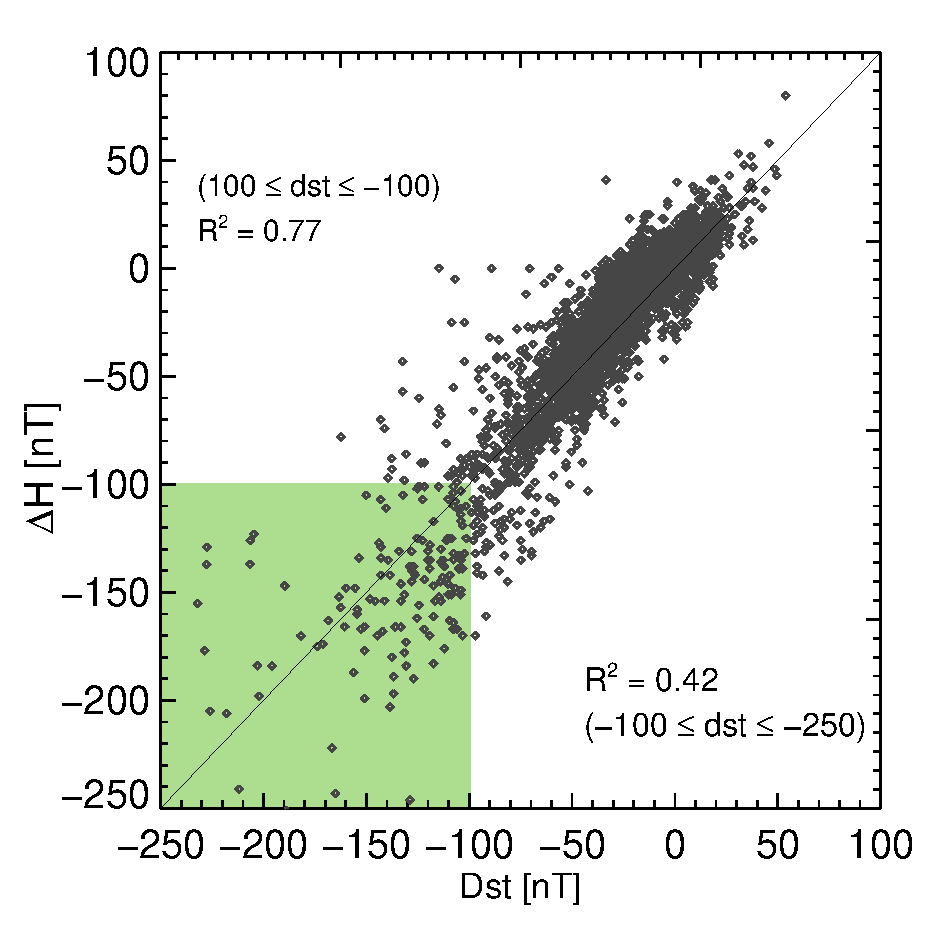
\includegraphics[width=0.45\textwidth]{images/disp_dst_v_dh/dispersion_general_dst.eps}
      \caption{Dispersion plot of regional and planetary geomagnetic responses as registered by $\Delta H$ (vertical axis) and $Dst$ (horizontal axis) for all anlyzed events. The figure also shows the correlation indices for data with $Dst \ge -100\, {\rm nT}$ and $-250 {\rm nT}\le Dst < -100\, {\rm nT}$ (shadowed-green region).}
       \label{fig:disp}
\end{figure}


Figure \ref{fig:disp} shows, in the case of our analyzed events, that planetary and regional geomagnetic indices may significantly differ each other. Which in turn suggests the presence of some kind of local (ionospheric) mechanisms with the capability to deviate the regional value of geomagnetic field from its planetary counterpart. Hence, we need to identify in the regional geomagnetic registers the signatures for the magnetic contribution cause by those local mechanisms \citep{ddyn2005, angeoddyn, amorymazaudier_2017, amory2020_filtros}. Now we proceed to identify such mechanisms.


%Our event selection criteria included ${\rm \Delta H_{TEO} \le -120~nT}$ and digital TEO register availability (from 2014-2019, and scatter and discontinuous periods from 2002 to 2013). Additionally, our analysis procedure requires data registers to be almost absent of data gaps, reason for which we set a threshold of $5\%$ to dismiss events with larger amount of data gaps. The selected events, as well regional and planetary properties, are listed in Table \ref{table1:GS_descp}.


%\subsection{Regional response \emph{vs} planetary activity}


%Now we proceed to verify the existence of differences between regional and planetary geomagnetic responses in the events listed in Table \ref{table1:GS_descp}. In order to do so, we search for differences between regional and planetary geomagnetic indices, since those differences may imply the presence of local geomagnetic response. Thus, we perform a correlation between ${\rm Dst}$ and $\Delta {\rm H_{TEO}}$ geomagnetic indices, where the regions of low correlation would imply confirmation of those commented differences and, in consequence, local geomagnetic response.

%Geomagnetic indices can be used to detect the geomagnetic response, however this will be quite different at global and regional scales. Differences in behavior for both, local and global geomagnetic indices, can imply the presence of local geomagnetic effects. Hence the first step is studying these differences.

%We compare the differences for global and local geomagnetic response by performing an analysis of dispersion and correlation between global and local geomagnetic indices. From the resulting data, we expect a decrement in correlation with respect to even more negative Dst values. Decrement in correlation values for different Dst ranges, and dispersion of data points imply the presence of significant geomagnetic local effects.
%. In general, we consider there are three kinds of differences between the local and planetary geomagnetic responses:  

%\begin{enumerate}
%    \item     Differences in magnitude of the minimum.
%    \item     Difference in the time arrival of the minimum. 
%    \item     Difference in behavior during the recovery phase. 
%\end{enumerate}
  

%The variability of the geomagnetic field behavior during a GS at local scale compared with the global scale resulting in these 3 differences have been studied for a while [cite] and their origin can be related to the local time [cite] in which the GS is originated, the trigger event and the local ionospheric response.

\subsection{Geomagnetic signatures of local ionospheric currents}
\label{diono}

The local values of $EMF$ are result from the contribution of many sources \citep{1969intro_to_iono_p, l_handbook_geof_sw_Geom_field,  baseline_Gjerloev, vanKampt}. In the particular case of the horizontal component ($H$) of local $EMF$, we can express it as:
\begin{equation}
    \label{eq:1}
    H = B_{SQ} + H_0 + D_{M} + D_{I}.
\end{equation}
With $B_{SQ}$ is the diurnal variation obtained from the local quiet days \citep{vanKampt} and $H_0$ is the day-to-day variation \citep{baseline_Gjerloev, vanKampt}. The last two terms are irregular magnetic variations related to geomagnetic activity \citep{ddyn2005, angeoddyn}, with $D_M$ being the contribution from (planetary scale) magnetospheric currents, and $D_I$ is the magnetic contribution driven by ionospheric perturbations. In addition, since we are at mid and low latitudes, $D_M \approx Dst \cos(\lambda)$, with $\lambda$ being the geomagnetic latitude \citep{amorymazaudier_2017}. Therefore, we can express $D_I$ as: 
\begin{equation}
\label{eq:diono}
   D_{I} \approx H -(B_{SQ} +  H_0 + Dst \cdot cos(\lambda)).
\end{equation}
Furthermore, we can also express $D_{I}$ as:
\begin{equation}
\label{eq:diono_explicit}
   D_{I} = DP2 + Ddyn + D_{others},
\end{equation}
Where $D_{\text{others}}$ refers to ionospheric perturbations distinct from the disturbed polar current number 2 ($DP2$) and the disturbed dynamo current ($D_{\text{dyn}}$). These two ionospheric currents are well accepted sources for local geomagnetic fluctuations in low and mid geomagnetic latitudes, as discussed in the Introduction.


% ---------------------------------------------------
% ---------->    SECTION    <----------
% ---------------------------------------------------
\section{Analysis and results}
\label{results}

\subsection{Local ionospheric disturbances and induced magnetic fluctuations}
\label{analysis}
In this section, we present our analysis process through showing the analysis of events 3, 6, 13 and 18. The panels (a) of Figure \ref{fig:iono_resp} show the profiles of $Dst$ (black) and $\Delta H$ (green) indices during the storm period associated with events (see Table \ref{table1:GS_descp}). In the panels we observe that both indices are \emph{quiet} up to the start of the $GS$'s main phase, signed out by a (left-sided) vertical dotted line. The main phase provokes the values of $Dst$ and $\Delta H$ indices to decrease up to reaching a minimum. Once this minimum value is reached, start the recovering phases where the magnetic indices slowly tend to recover their \emph{quiet} (pre-storm) value. This phase regularly extends for several hours or even days up to the end of the $GS$ (right-side vertical dotted line).  

\begin{figure*}[h!]
	\centering
	\centerline{\Large \bf   
		%\hspace{0.18\textwidth}  \color{black}{\Large{Res}}
		%\hspace{0.28\textwidth}
		%\color{black}{\Large{Res+TC}}
		\hfill}
	\centerline{\Large \bf   
		\hspace{0.26\textwidth}  \color{black}{}
		\hspace{0.31\textwidth}  \color{black}{}
		\hfill}
	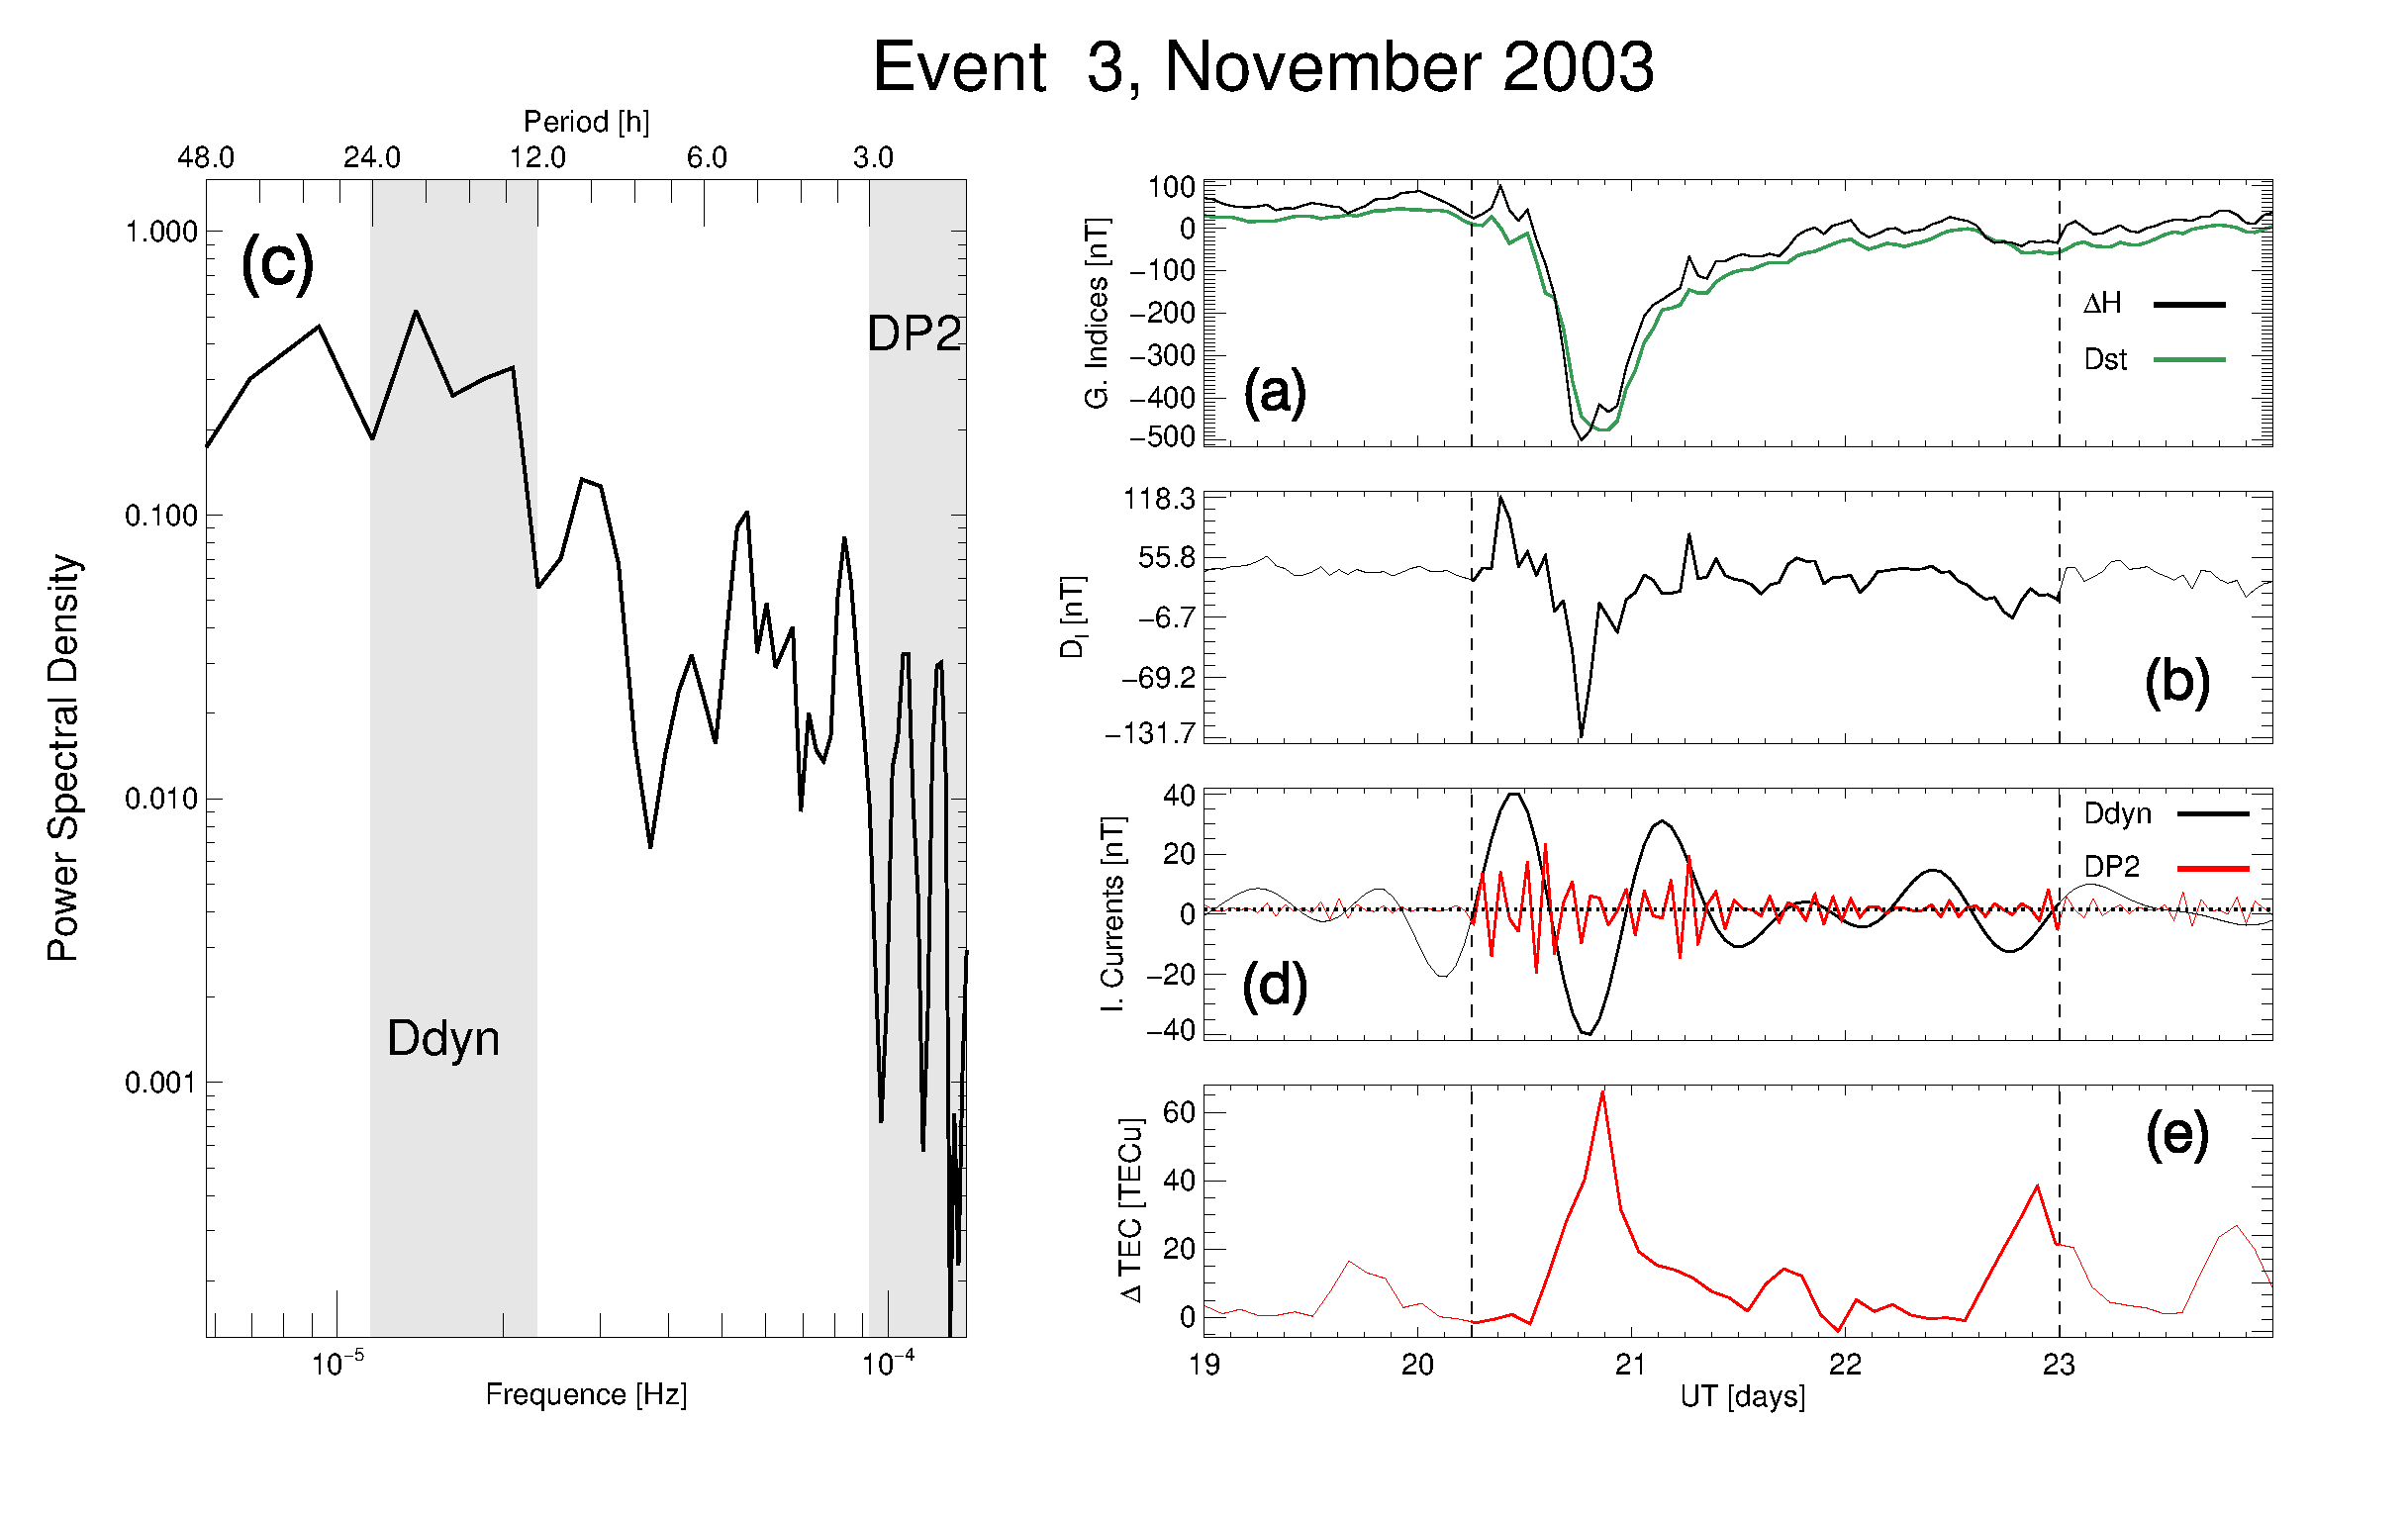
\includegraphics[width=0.45\textwidth]{images/diono/iono_PI_2003-11-19.eps}
	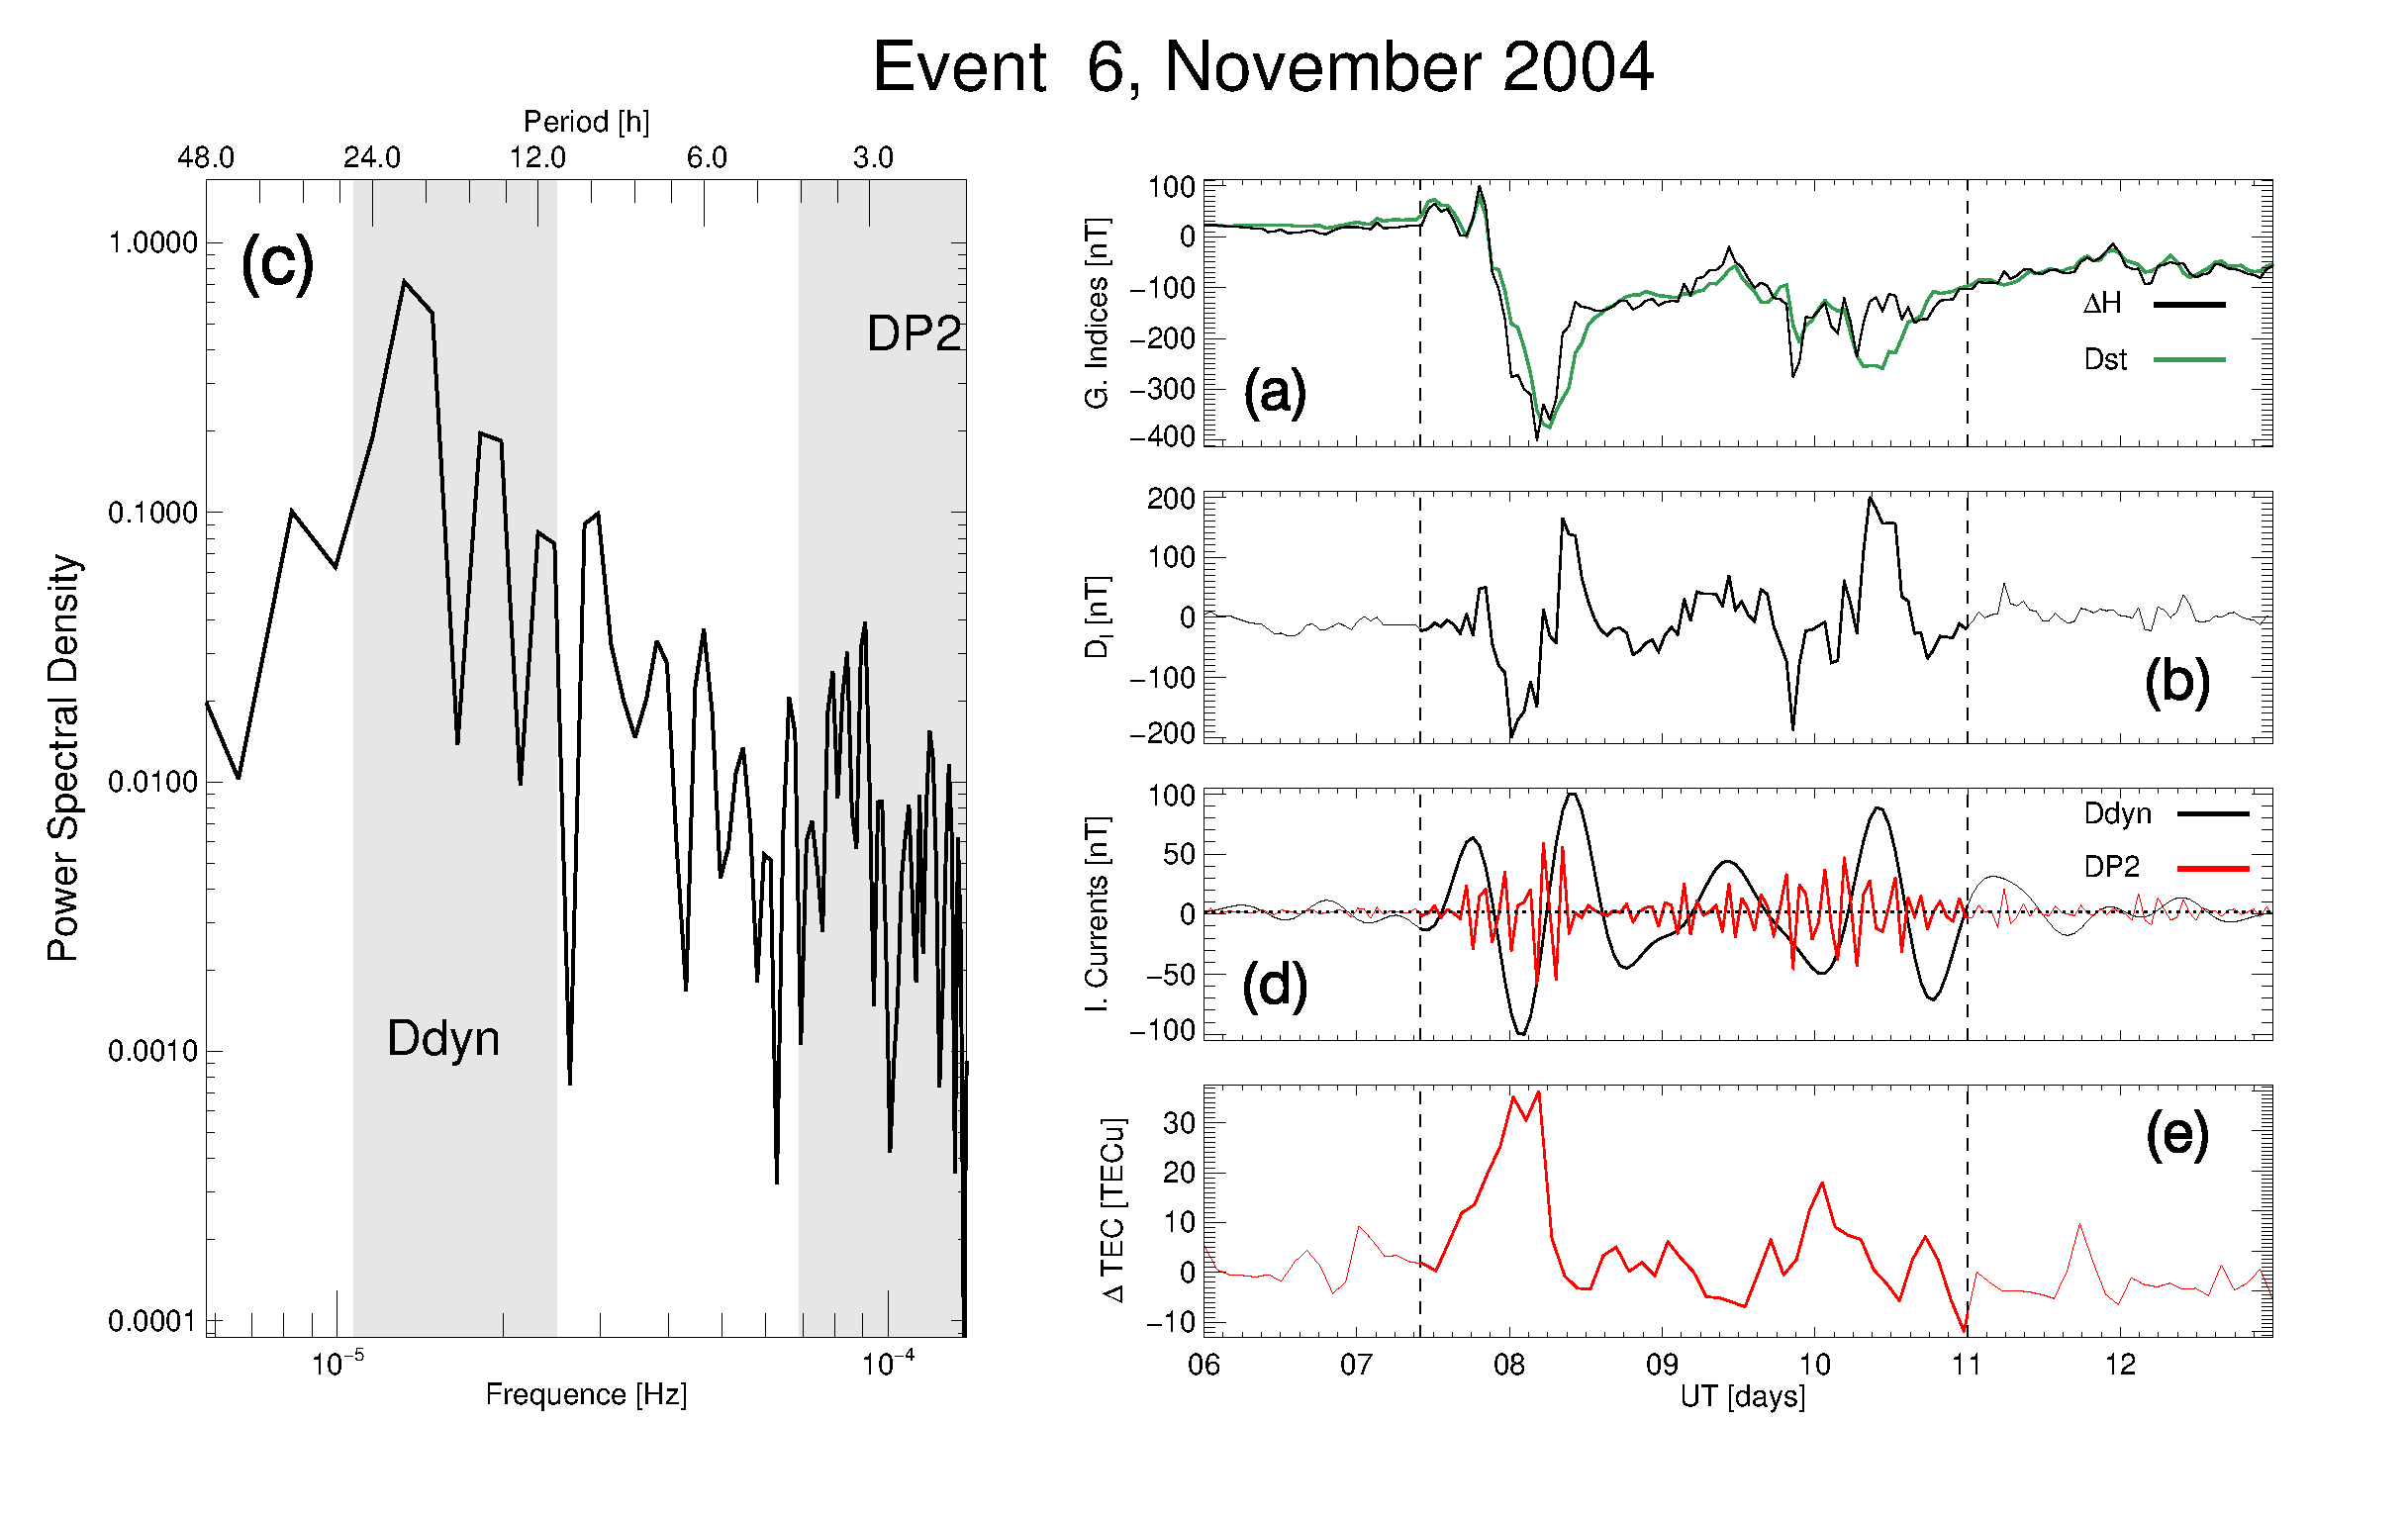
\includegraphics[width=0.45\textwidth]{images/diono/iono_PI_2004-11-06.eps}

	\centerline{\Large \bf   
	\hspace{0.26\textwidth}  \color{black}{}
	\hspace{0.31\textwidth}  \color{black}{}
	\hfill}	   
	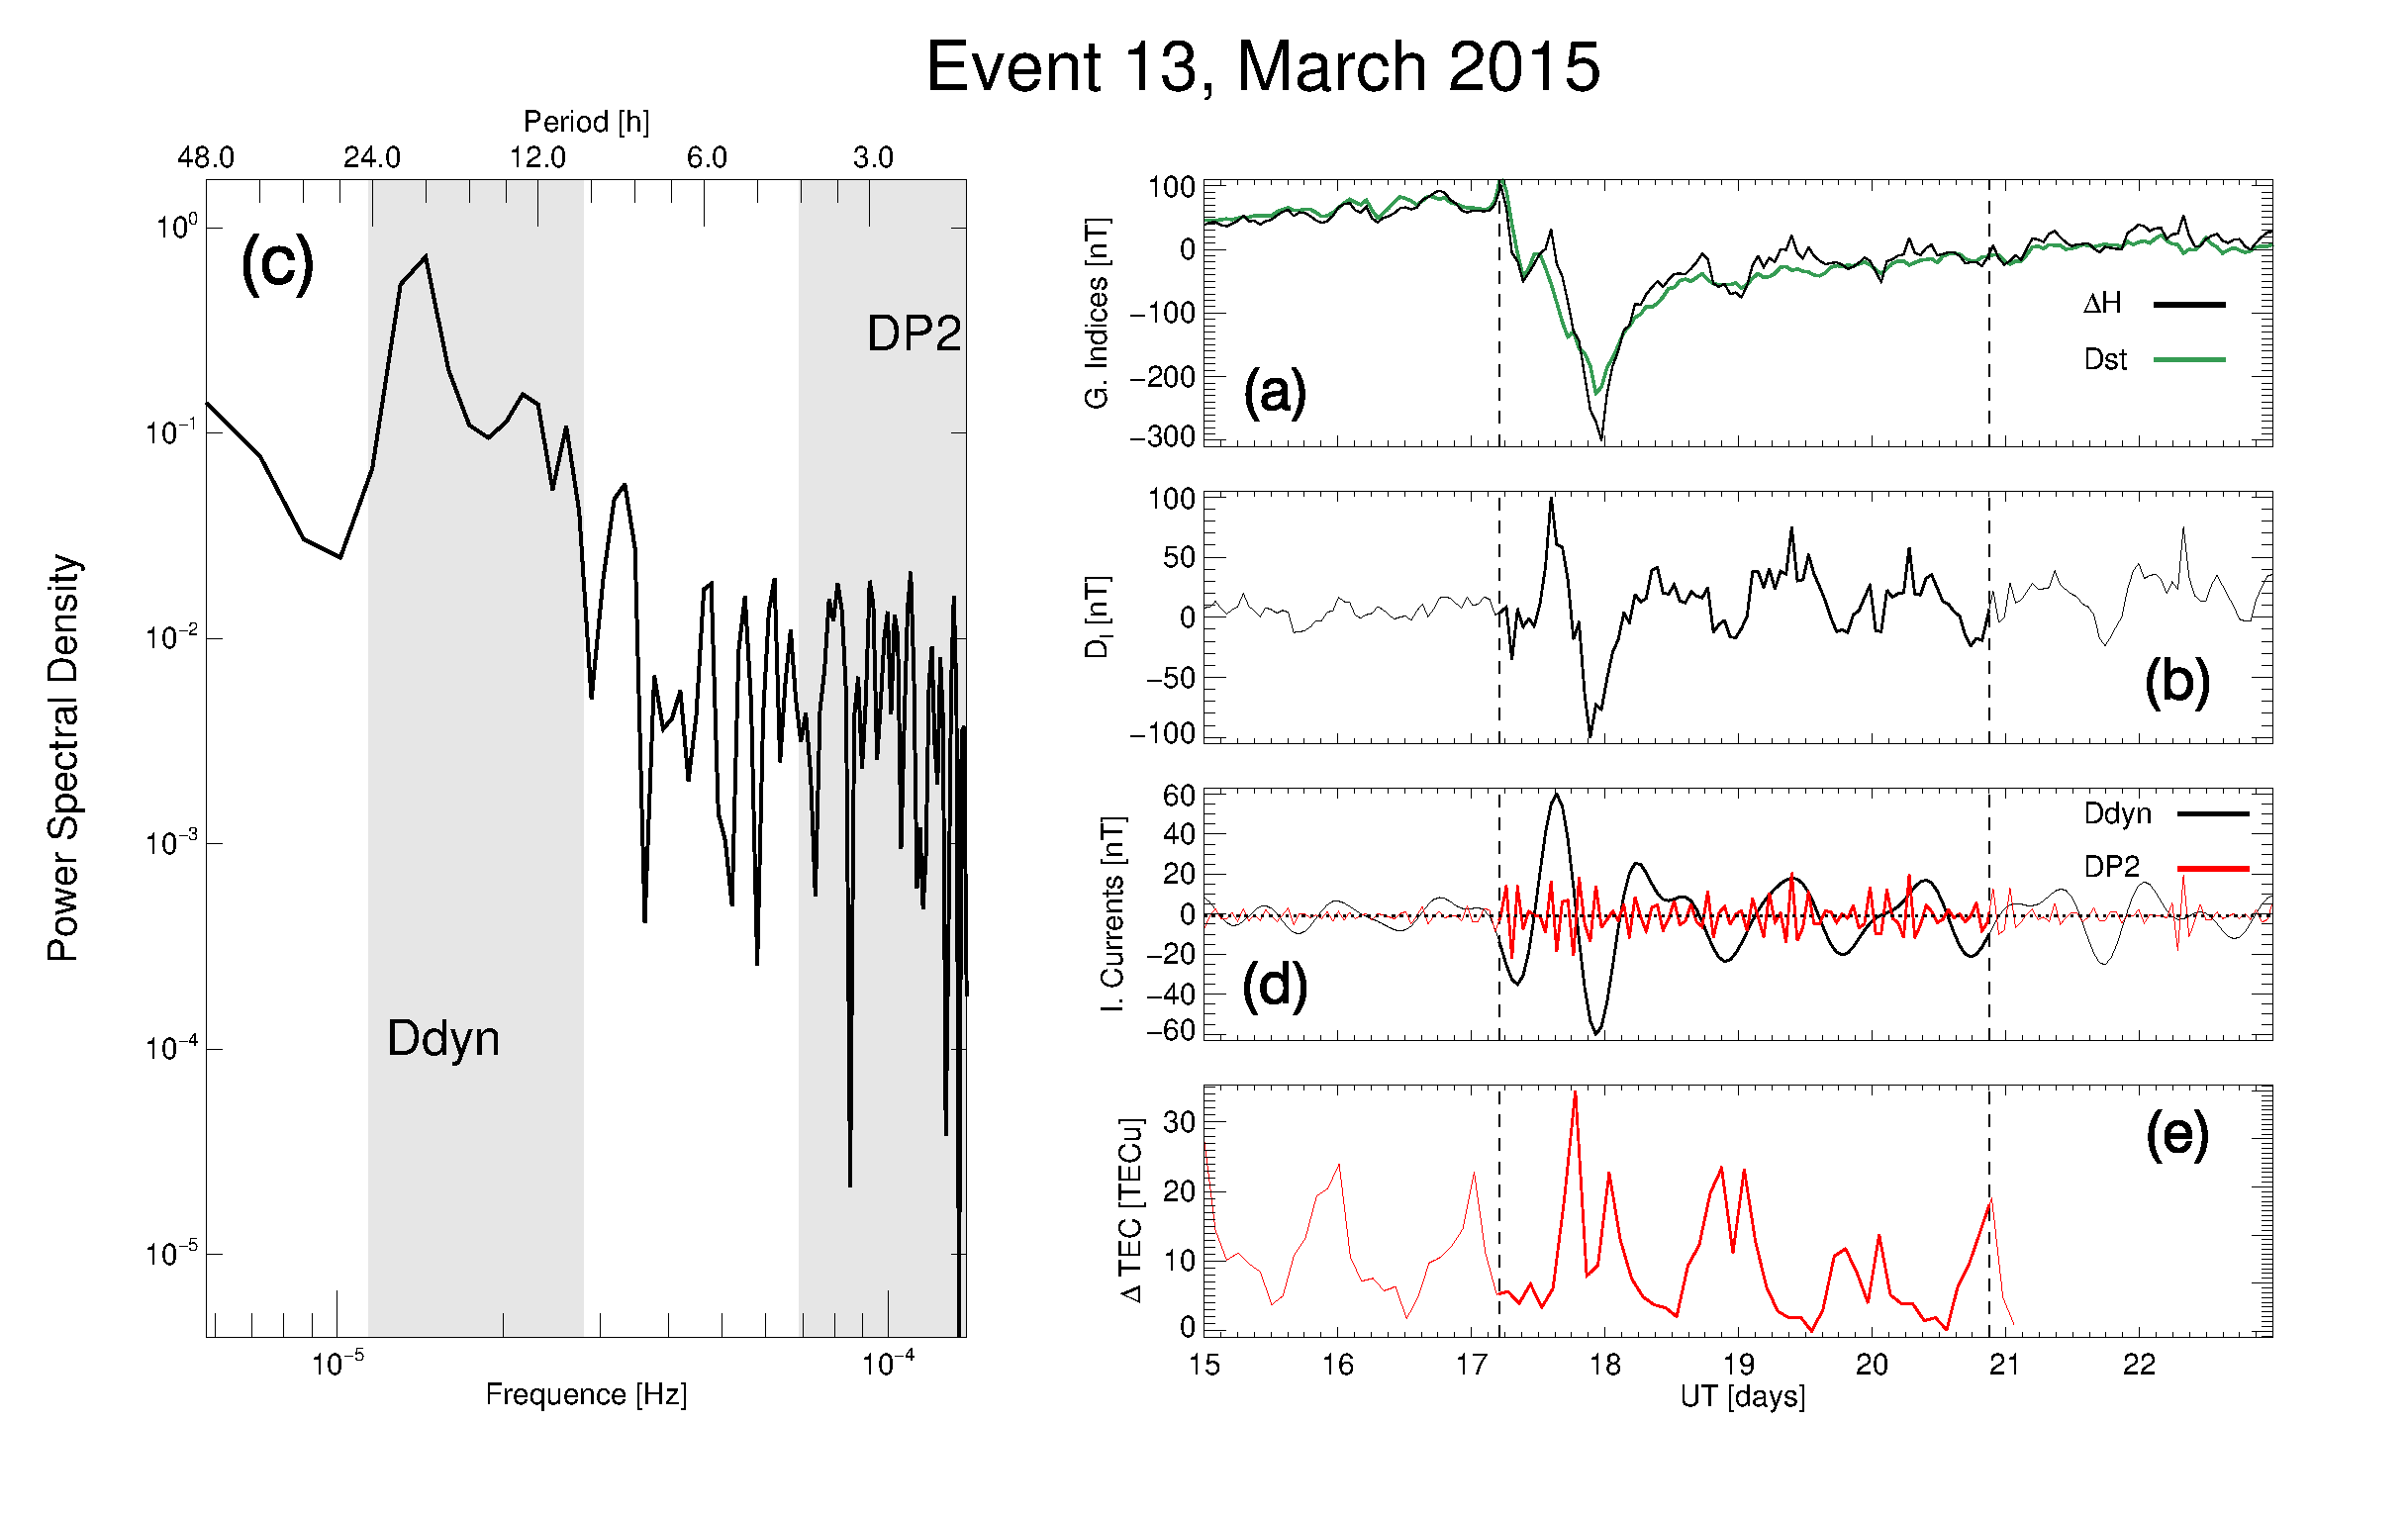
\includegraphics[width=0.45\textwidth]{images/diono/iono_PI_2015-03-15.eps}
    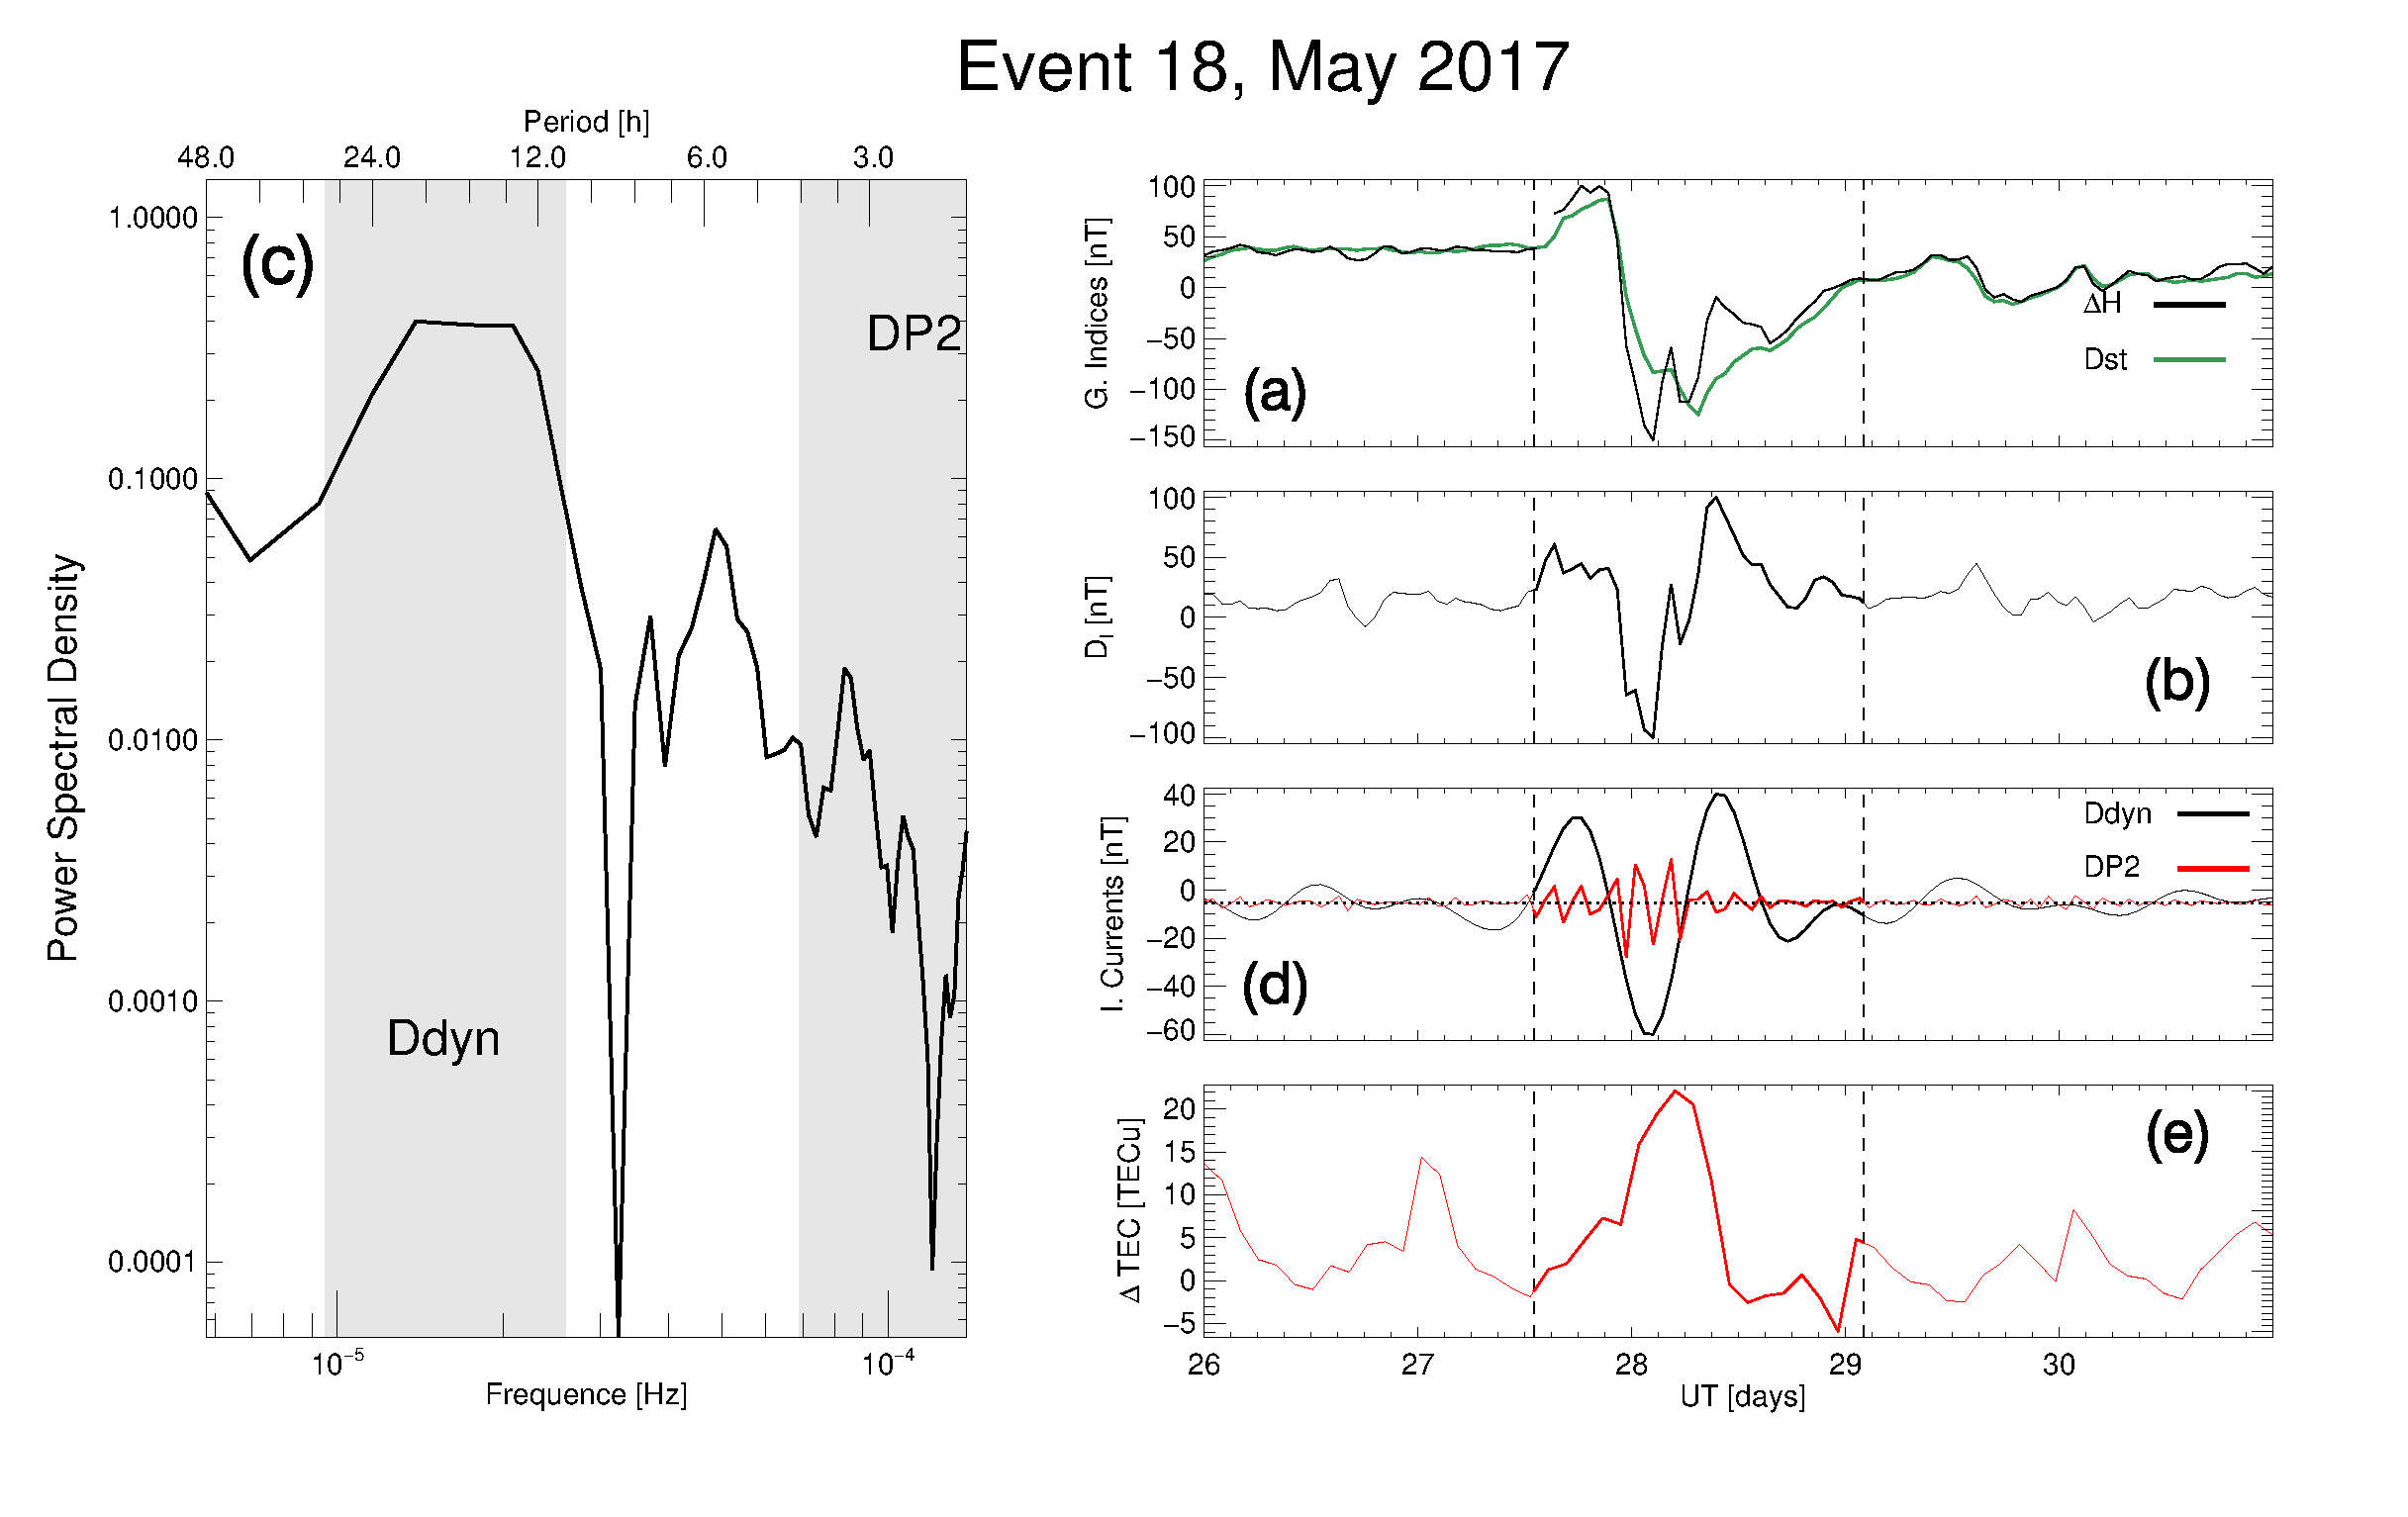
\includegraphics[width=0.45\textwidth]{images/diono/iono_PI_2017-05-26.eps}   	
    
    
	\caption{Analysis examples from solar cycle 23 (upper panels) and solar cycle 24 (bottom panels). Upper(bottom) panels show the analysis of events 3(13) and 6(18). The analysis of each event is make up of five different processes representd by panels labeled with letters. Panels (a) present the values of $Dst$ (black line) and $\Delta H$ (green line) indices during the event. Panels (b) show the computed value of $D_I$. Panels (c) show the power spectrum associated to $D_I$. Panels (d) show the the induced geomagnetic effects of $Ddyn$ (in black) and $DP2$ (in red) reconstructed from the filtered power spectrum. Panels (e) show the variation of the total electron content ($\Delta TEC = TEC - <TEC>$) over the central region of Mexico. The dotted vertical lines in panels (a), (b), (d) and (e) mark out the start (left-sided) and end (right-sided) of the $GS$. Gray shaded regions in panel (c) highlight the bandwidths associated with $Ddyn$ and $DP2$ filters.}
	\label{fig:iono_resp}
\end{figure*}


In the panels (b) of Figure \ref{fig:iono_resp}, we appreciate the resulting profile of $D_I$ (Equation (\ref{eq:diono})), which we computed using the $\Delta {H}$ and the $Dst$ reported data. It is remarkable that all $D_I$ profiles shown in Figure \ref{fig:iono_resp} significantly differe each other. Subsequently, we compute the power spectrum of each $D_I$, which we show in panels (d) of Figure \ref{fig:iono_resp}. In the power spectra, we highlight, by a gray shading, the range of periods(frequencies) consistent with $DP2$ and $Ddyn$. It is important to comment that we manualy identify $Ddyn$'s range by setting the main period and searching potency peaks within the range of possible harmonics. These slightly variations on periods(frequencies) are due to the differences between our study cases, already commented.

In panels (c) of Figure \ref{fig:iono_resp} we present the profiles of the induced magnetic perturbations caused by $DP2$ (solid red line) and $Ddyn$ (solid black line). These profiles are constructed departing from the frequencies identified through the filtering process commented on in the previous paragraph. We note that the enhancements of the induced effects of $Ddyn$ and $DP2$ simultaneously occur with significant variations in the total electron content ($\Delta TEC$) over central Mexico, as the panels (e) of Figure \ref{fig:iono_resp} shows.

We applied the procedure described in this section to all our study cases. The Figures \ref{fig:iono_resp2} and \ref{fig:iono_resp3} in the Appendix \ref{apend} show the results from our analysis. In general, we noted that the amplitude of the magnetic oscillations induced by $Ddyn$ tend to be larger than those induced by $DP2$ (see Figures \ref{fig:iono_resp2} and \ref{fig:iono_resp3} at the Appendix  \ref{apend}). This suggests that, in most cases, the intensity of $Ddyn$'s induced magnetic effects are larger than those induced by $DP2$, and thus $Ddyn$'s effects are also dominant on the local $EMF$.

We believe that the process that triggers the $GS$ itself may affect the evolution of the ionospheric response, directly modifying the evolution of $DP2$ and $Ddyn$ currents. Secondly, we have to consider that our data is sampled in hourly resolution. In this case, data sampling represents an important limitation since $DP2$ magnetic fluctuations, as mentioned in \cite{nishida_68_fluctuations}, may have periods of less than an hour or even of tens of minutes. In this scenario, we possibly missed part of $DP2$ fluctuations and potency during our analysis. This could be solved, in principle, by using $Sym-H$ index rather than $Dst$, a task which exploration we consider as future work.

 

%%%%%%%%%

%In the panel (b) of Figure \ref{fig:iono_resp}, we appreciate the resulting profile of $D_I$ (Equation (\ref{eq:diono})), which we computed using the TEO's registers and the $Dst$ reported data. Subsequently, we construct a power spectrum for our computed profile of $D_I$, which we show in panel (d) of Figure \ref{fig:iono_resp}. In the power spectrum, we highlight, by a yellow shadowing, the range of periods(frequencies) consistent with $DP2$ and $Ddyn$. In the panel, we identify $Ddyn$'s range by setting the main period and searching potency peaks within the range of possible harmonics. It is important to remark that, because our study cases might be potentially different from each other, the filtering ranges might vary slightly from case to case.

%In Figure \ref{fig:iono_resp}(c) we present the profiles of the induced magnetic perturbations caused by $DP2$ (solid red line)Geomagnetic Storm  and $Ddyn$ (solid black line). These profiles are constructed departing from the frequencies identified through the filtering process commented on in the previous paragraph. We note that the enhancements of the induced effects of $Ddyn$ and $DP2$ simultaneously occur with an increase in the total electron content over central Mexico, as the panel (e) of Figure \ref{fig:iono_resp} shows.

%We applied the procedure presented in this section to all our study cases. The Figures \ref{fig:iono_resp2} and \ref{fig:iono_resp3} in the Appendix show the computed $D_I$ and the resulting profiles of $DP2$ and $Ddyn$, for each event in Table \ref{table1:GS_descp}. We remark on the uniqueness of each event, which is clear in the $D_I$ profiles and its associated magnetic perturbations induced by $DP2$ and $Ddyn$ currents.

%From Figures \ref{fig:iono_resp2} and \ref{fig:iono_resp3}, we note that generally, the amplitude of the magnetic oscillations induced by $Ddyn$ are more intense than those induced by $DP2$. This suggests that, in most cases, $Ddyn$'s induced magnetic effects are dominant on the local EMF. Although there are events for which both effects show similar intensities. We think of two possibilities to explain: The first is the process that triggers the GS itself, \emph{i.t.} the solar activity event, and its magnetic reconnection with the EMF. This may affect the evolution of the ionospheric response, directly modifying the evolution of $DP2$ and $Ddyn$ currents. Secondly, we have to consider that our data is sampled in hourly resolution. In this case, data sampling represents an important limitation since $DP2$ magnetic fluctuations, as mentioned in \cite{nishida_68_fluctuations}, may have periods of less than an hour or even of tens of minutes. In this scenario, we possibly missed part of $DP2$ fluctuations during our analysis. This could be solved, in principle, by using $Sym-H$ index rather than $Dst$, a task in which exploration we consider our future work.

\subsection{Validation of DP2 and Ddyn magnetic signatures}
\label{validation}

In Section \ref{local response} we were able to identify significant differences between the planetary and regional geomagnetic activity. Condition that we associated to regional geomagnetic response. Subsequently, in Section \ref{analysis}, we identified the tentative geomagnetic mechanisms for that regional geomagnetic response. Such mechanism are the $Ddyn$ and $DP2$ ionospheric currents, whose effects were reconstructed by a periods (frequencies) filtering process. We also learned that those effects are systematically associated with local perturbations on $TEC$. Now, we require to validate our results.

In order to validate our previous results, first we approximate the regional geomagnetic index $\Delta H$, which can be defined as:
\begin{equation}
    \label{eq:deltaH}
    \Delta H = H - (B_{SQ} + H_0),
\end{equation}
through $Dst$ and the resulting profiles of $DP2$ and $Ddyn$. Thus, by manipulating Equations (\ref{eq:diono}), (\ref{eq:diono_explicit}) and (\ref{eq:deltaH}) we obtain that:
\begin{equation}
    \label{eq:deltaHandDst}
    \Delta H \approx \cos(\lambda) Dst + DP2 + Ddyn.
\end{equation}
For simplicity, we call $ Dst_\lambda$ the combined effects of $ \cos(\lambda) Dst$, $DP2$ and $Ddyn$:
\begin{equation}
    \label{eq:Dstlambda}
    Dst_\lambda = \cos(\lambda) Dst + DP2 + Ddyn.
\end{equation}
In our context, $Dst_\lambda$ represents the combined effects of planetary geomagnetic response translated at the geomagnetic latitude ($\lambda$) of central Mexico and the regional geomagnetic effects of $DP2$ and $Ddyn$. Hence, our first step for validation is to corroborate that our computed value of $ Dst_\lambda$ approximates $\Delta H$. In addition, we can also used $ Dst_\lambda$ and the values of $K_p$ to approximate the local value of $K$.

The results of the validation process commented on before applied on events 3, 13 and $\&$ 18 are shown by Figure \ref{fig:iono_valid}. The upper panels of Figure \ref{fig:iono_valid} compares the profiles of $\Delta H$ (black), $Dst$ (green) and $Dst_\lambda$ (red). In the panel we note that $Dst_\lambda$ is systematically closer to $\Delta H$ than $Dst$. This condition holds during the main and recovering phases of the $GS$. %Additionally, in the bottom panels of Figure \ref{fig:iono_valid} it is clear that the planetary (green) and local (black) values of $K$ index differ each other.

%To simplify, we denote $ Dst_\lambda$ as the combined effect of $ Dst\cos(\lambda)$, $DP2$, and $Ddyn$. This leads to our first validation step, confirming whether the computed $ Dst_\lambda$ approximates $\Delta H$. Additionally, we employ $ Dst_\lambda$ and the values of $K_p$ to approximate the local $K$ value.

%Figure \ref{fig:iono_valid} portrays the validation process applied to event 13. The top panel juxtaposes profiles of $\Delta H$ (black), $Dst$ (green), and $Dst_\lambda$ (red). It is evident that $Dst_\lambda$ consistently tracks closer to $\Delta H$ than $Dst$, holding true during the main and recovery phases of the geomagnetic storm (GS). The bottom panel reveals that the values of planetary (green) and local (black) $K$ differ. However, when $Dst_\lambda$ is combined with $K_p$ values using uncertainty bars, the local $K$ profile generally falls within this range.


\begin{figure*}[h!]
	\centering
	\centerline{\Large \bf   
		%\hspace{0.18\textwidth}  \color{black}{\Large{Res}}
		%\hspace{0.28\textwidth}
		%\color{black}{\Large{Res+TC}}
		\hfill}
	\centerline{\Large \bf   
		\hspace{0.26\textwidth}  \color{black}{}
		\hspace{0.31\textwidth}  \color{black}{}
		\hfill}
	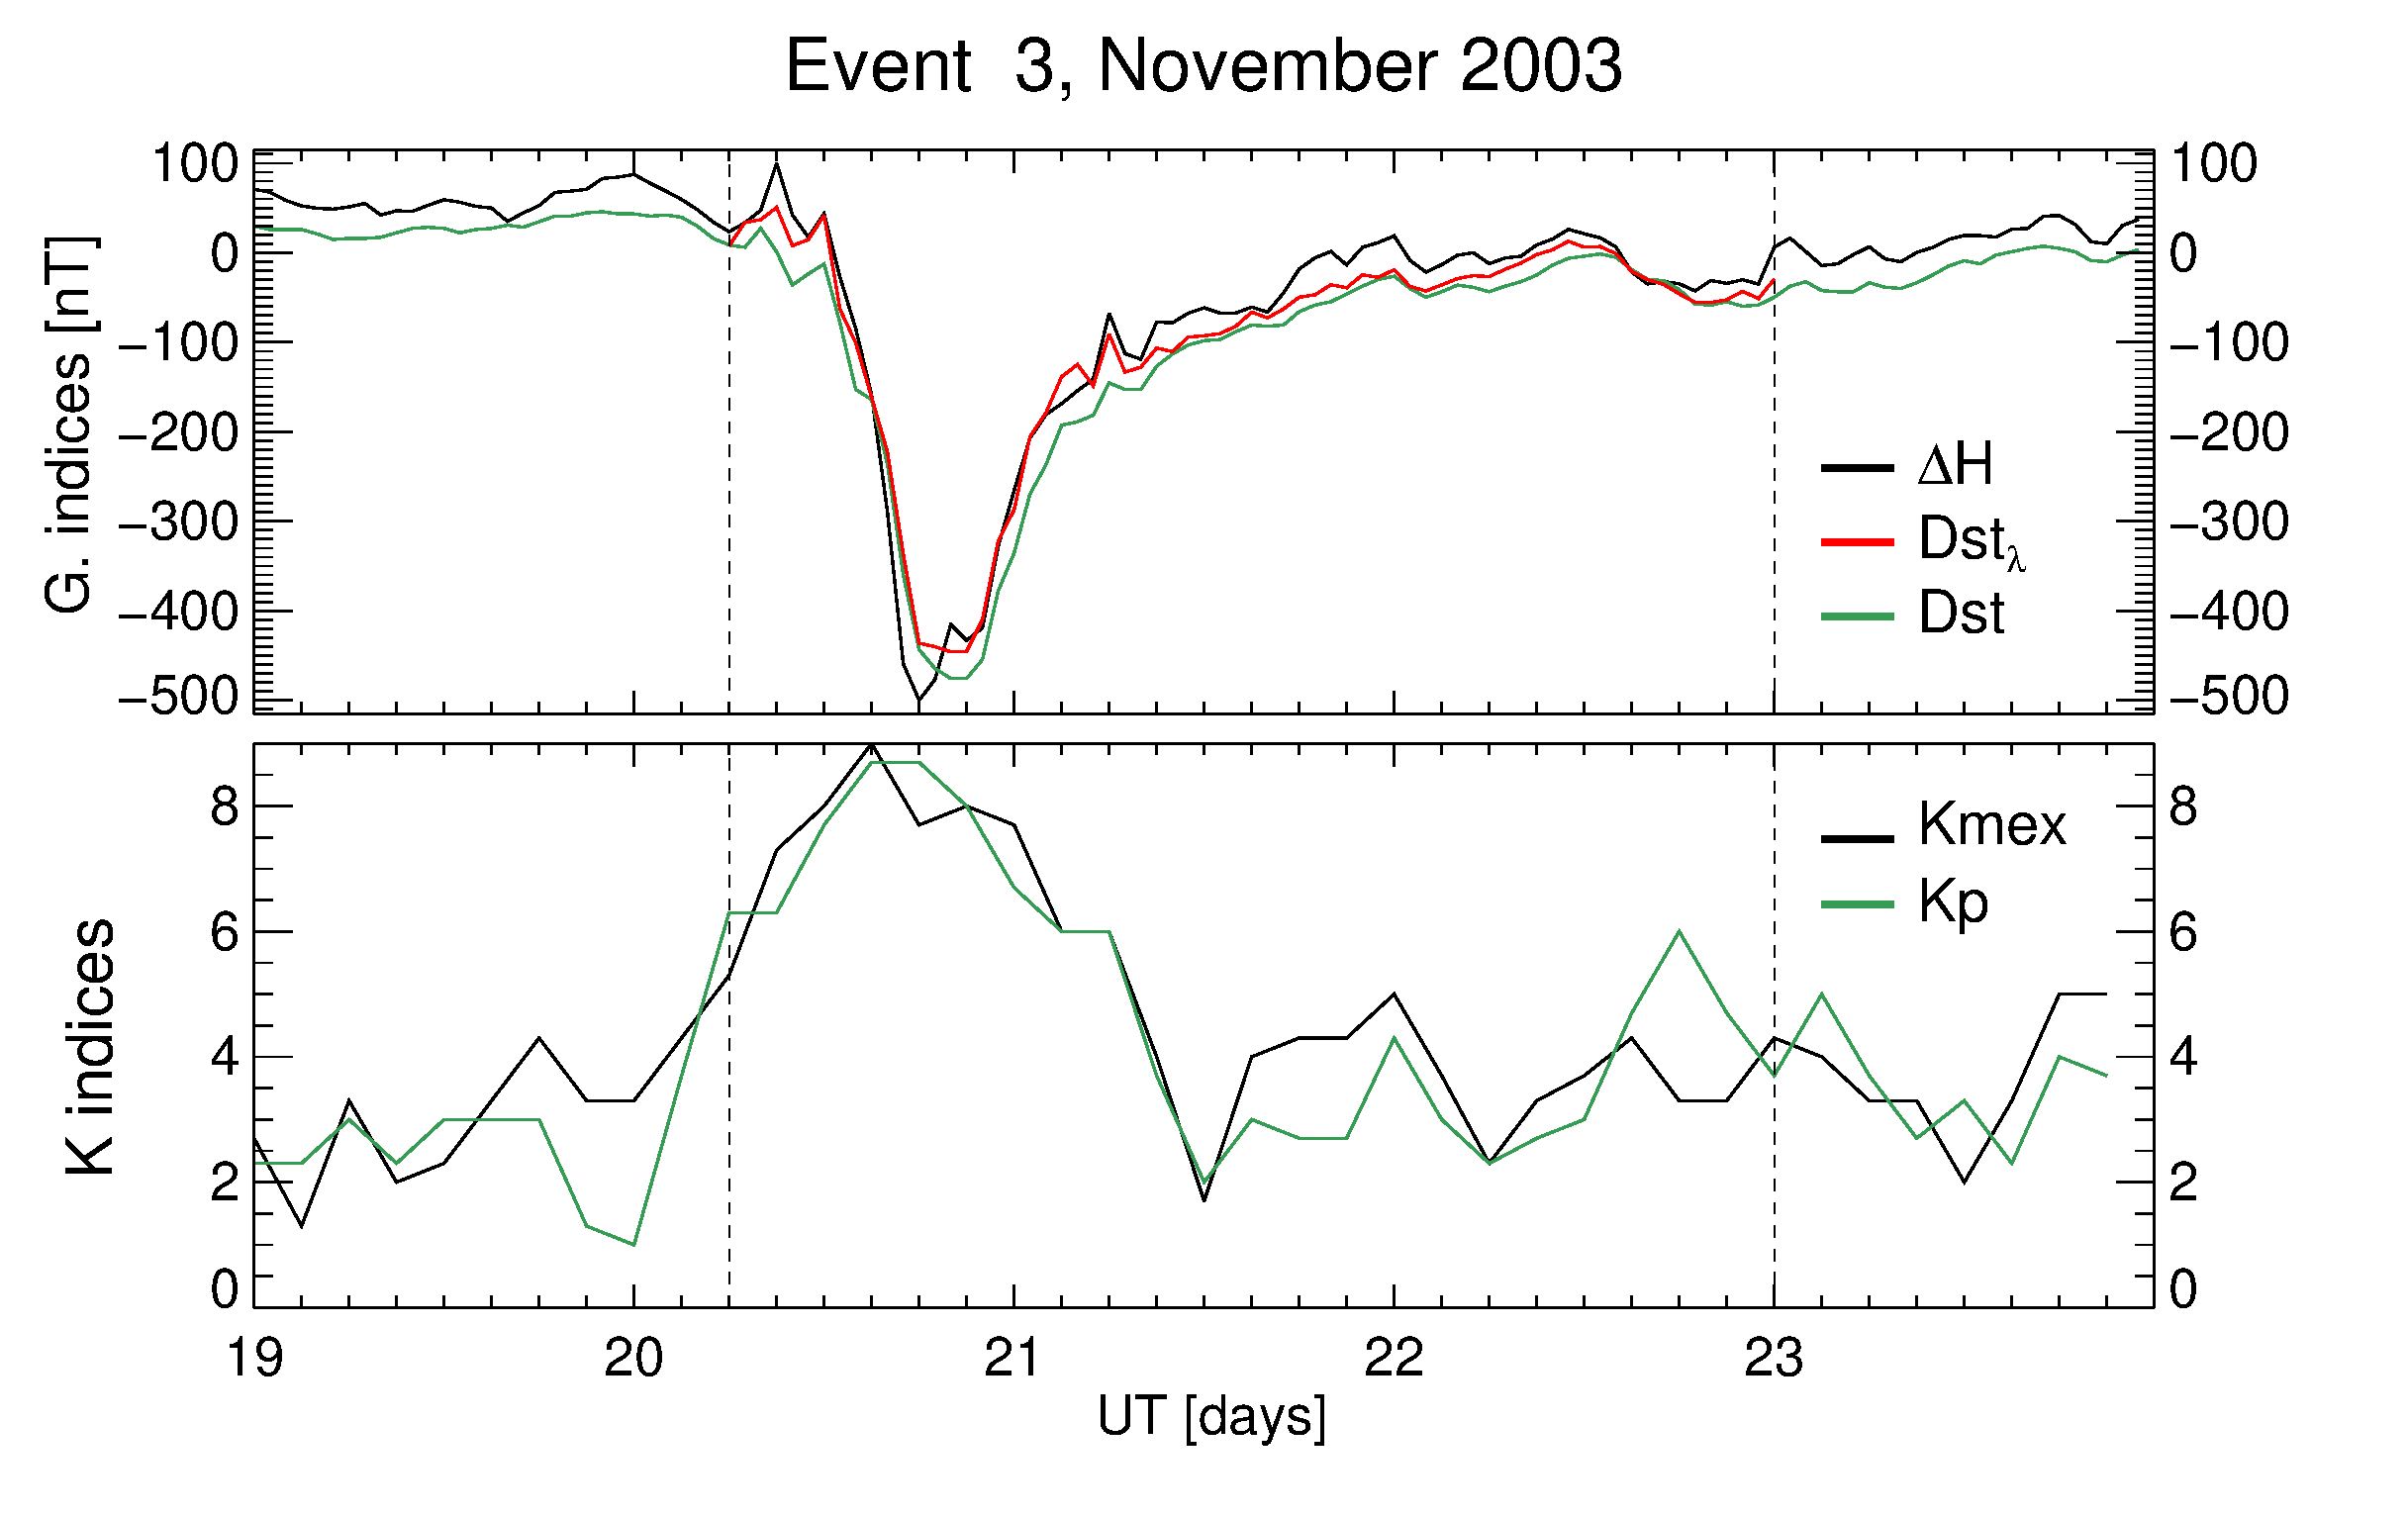
\includegraphics[width=8.0cm]{images/dH_approx/diono_valid_V4_2003-11-19.eps}
	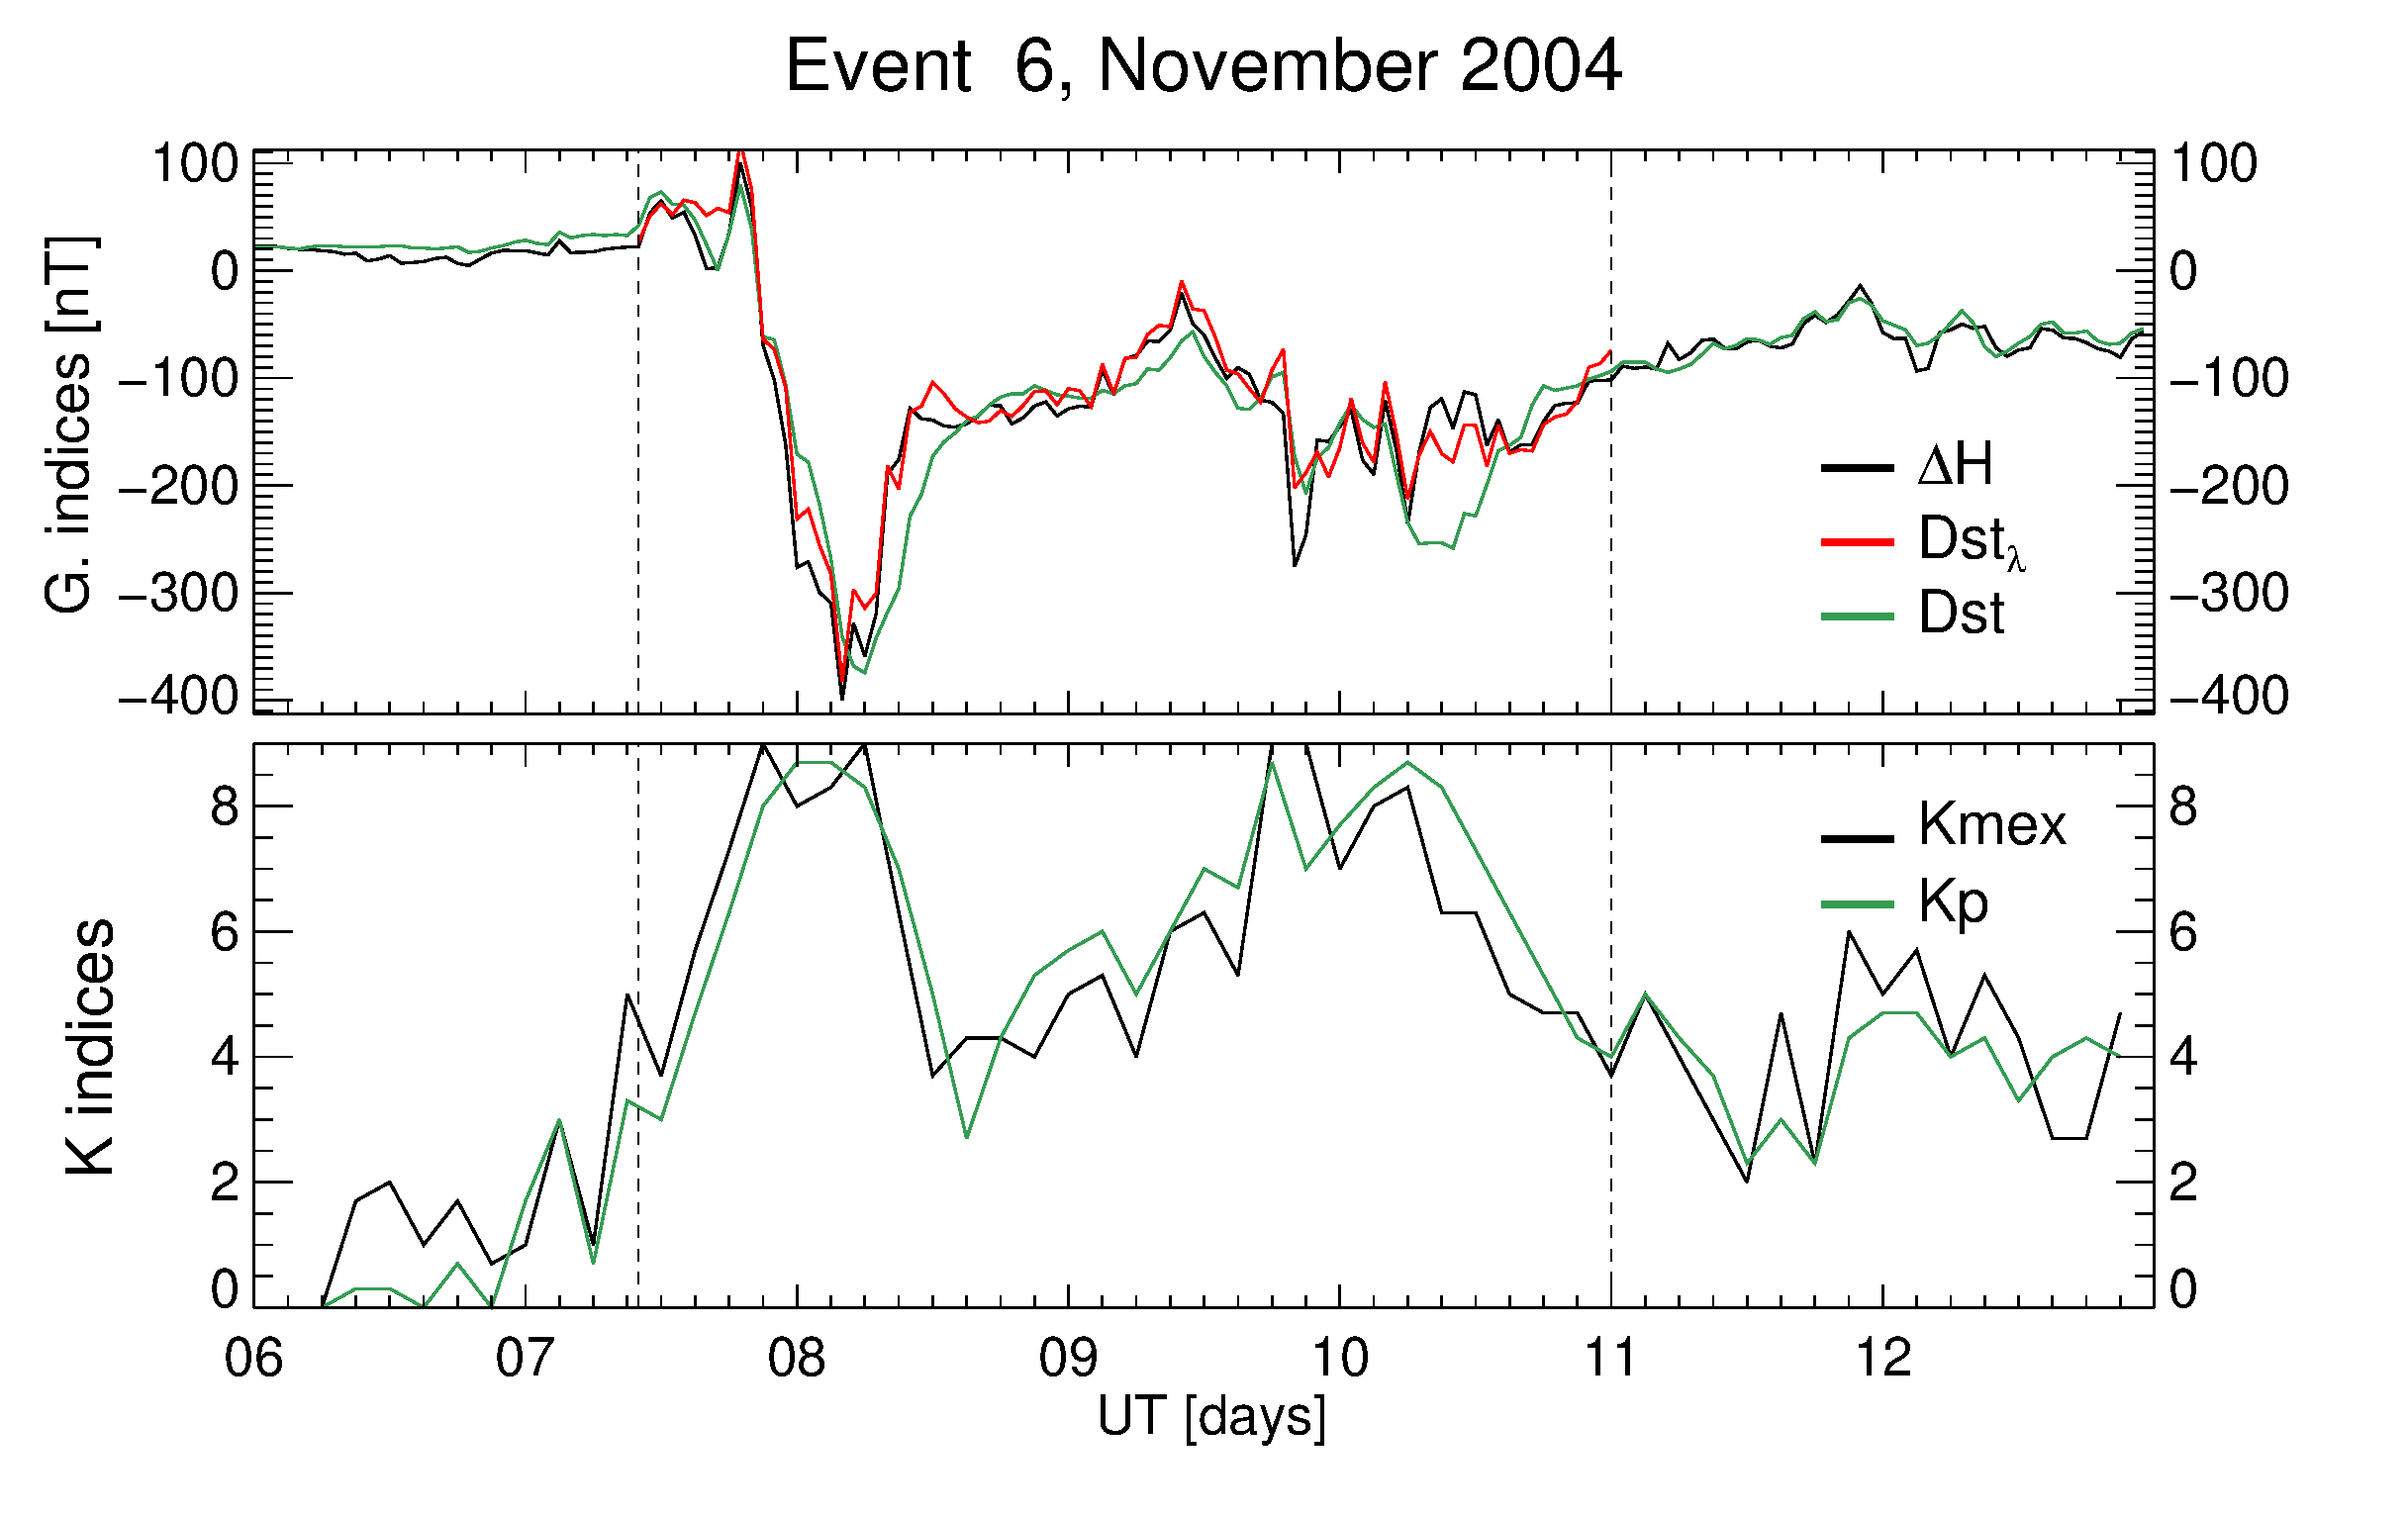
\includegraphics[width=8.0cm]{images/dH_approx/diono_valid_V4_2004-11-06.eps} 		

	\centerline{\Large \bf   
	\hspace{0.26\textwidth}  \color{black}{}
	\hspace{0.31\textwidth}  \color{black}{}
	\hfill}	   
	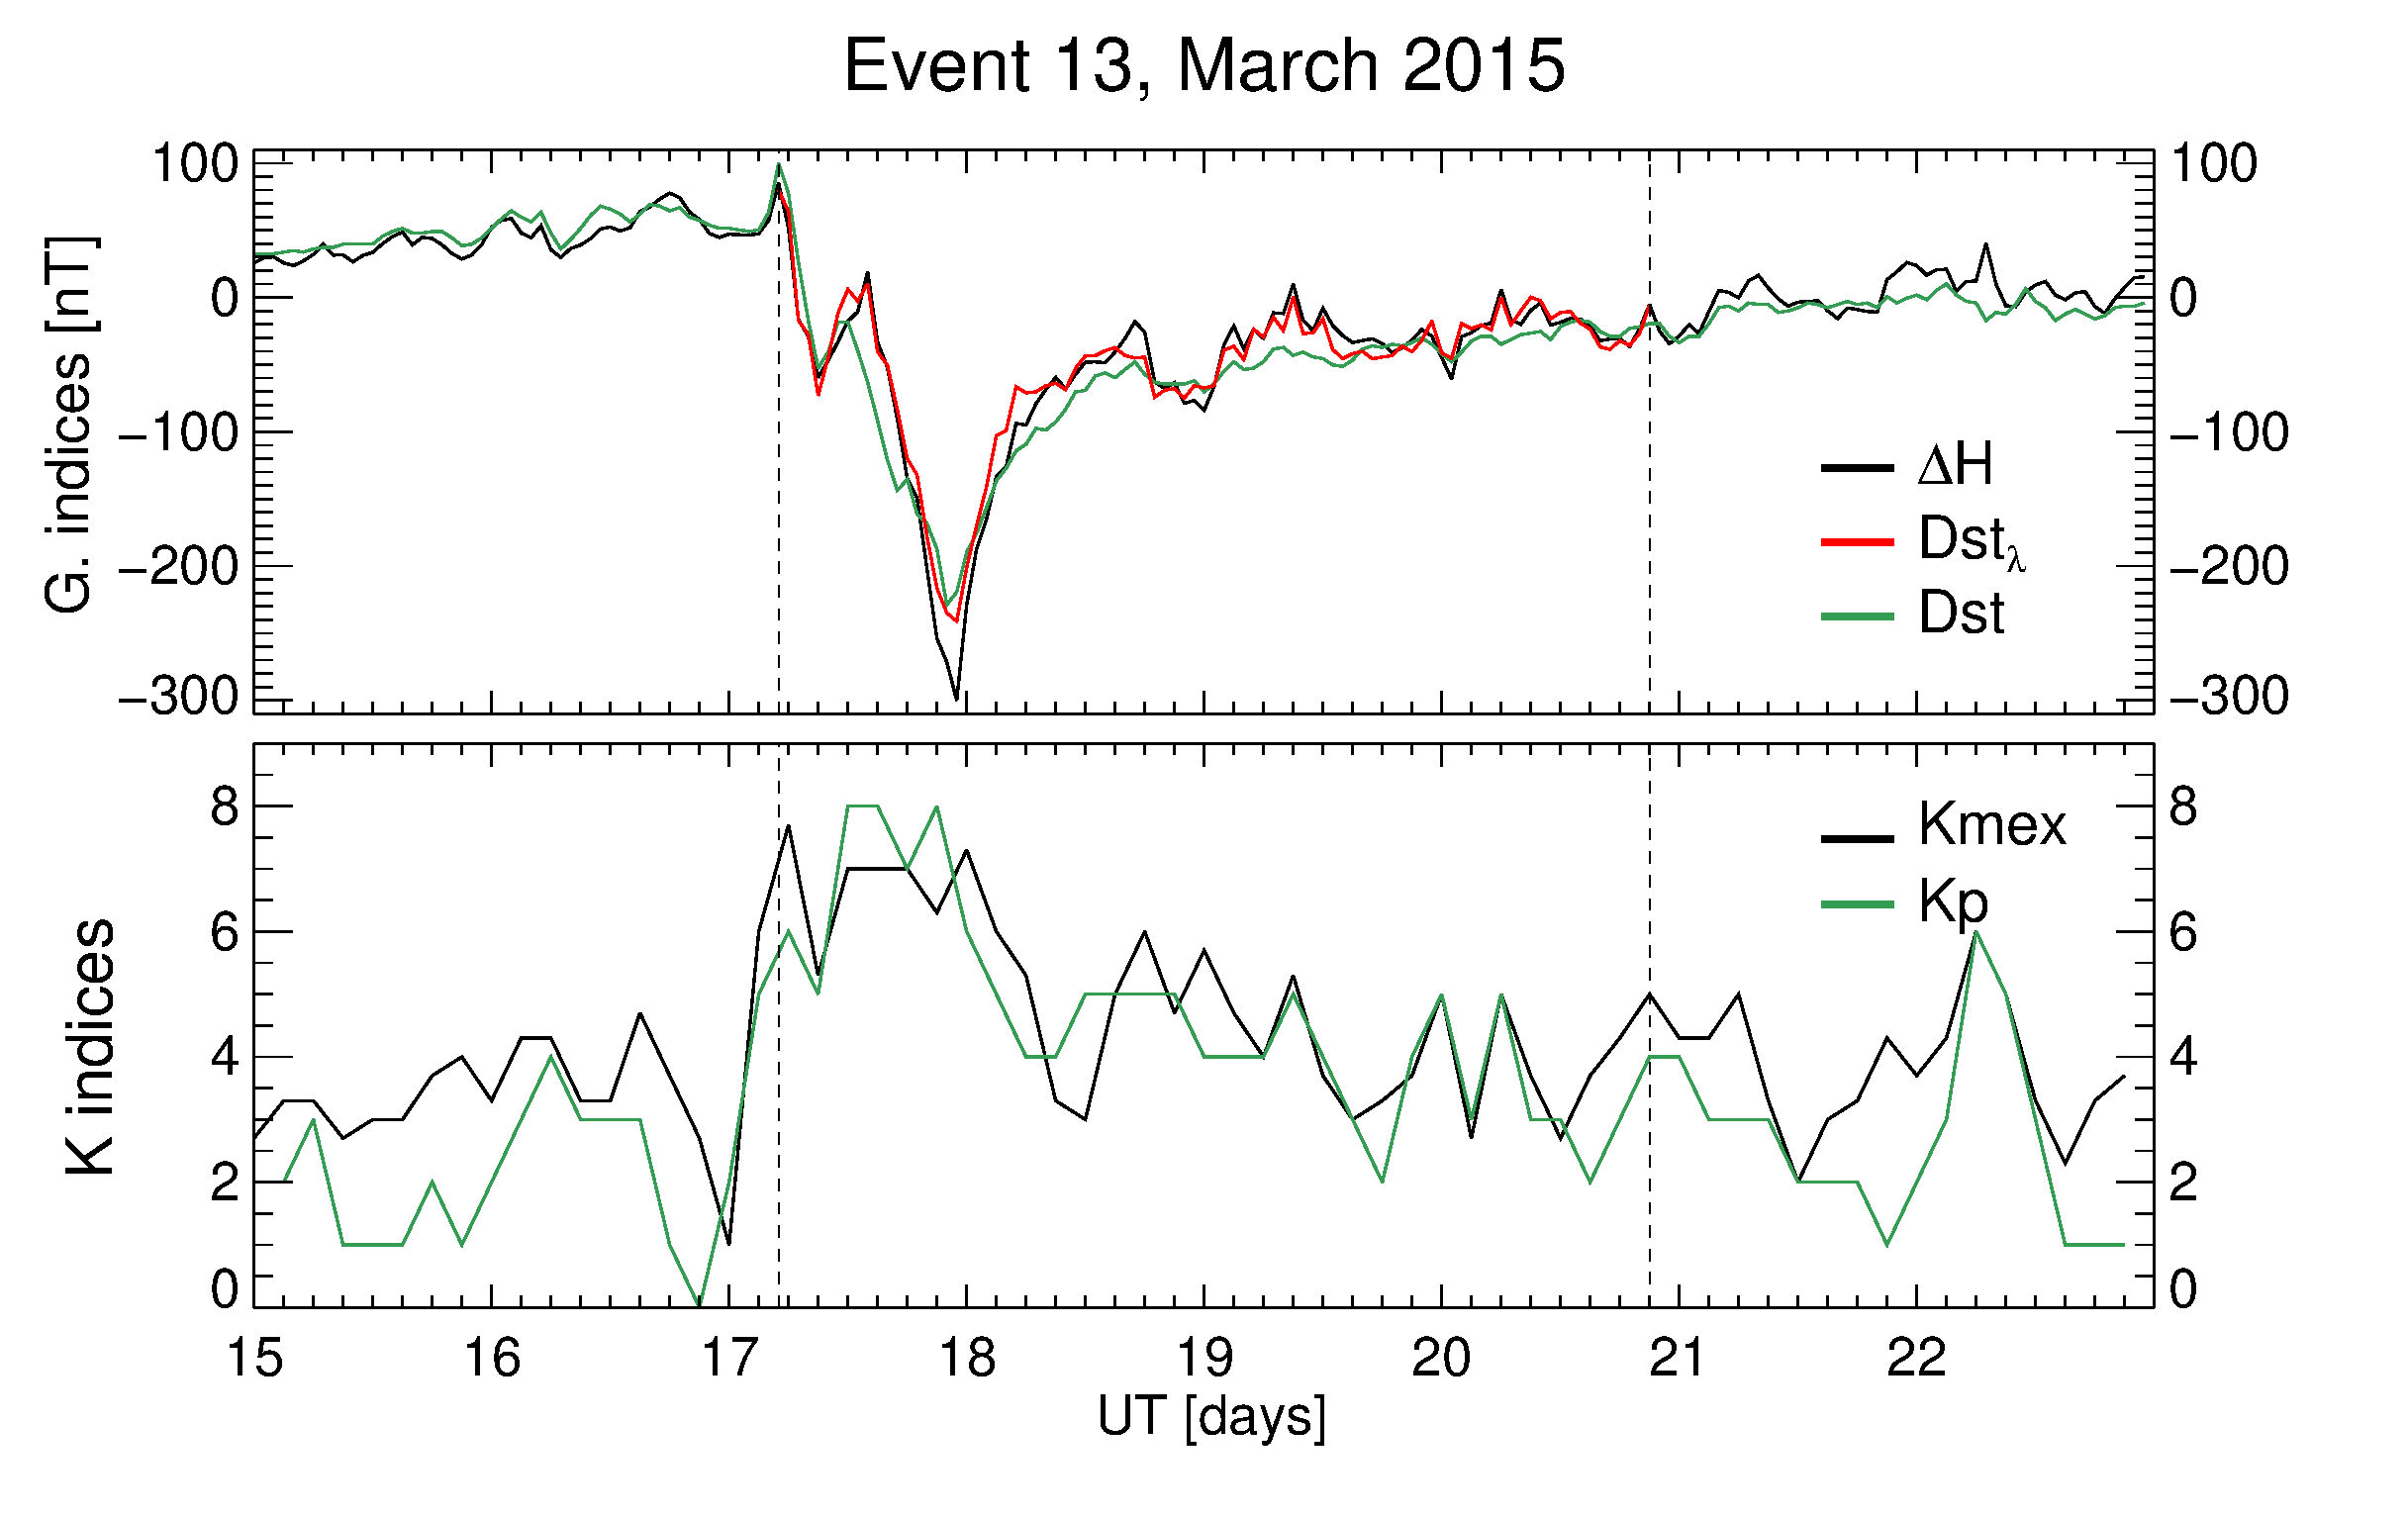
\includegraphics[width=8.0cm]{images/dH_approx/diono_valid_V4_2015-03-15.eps}
	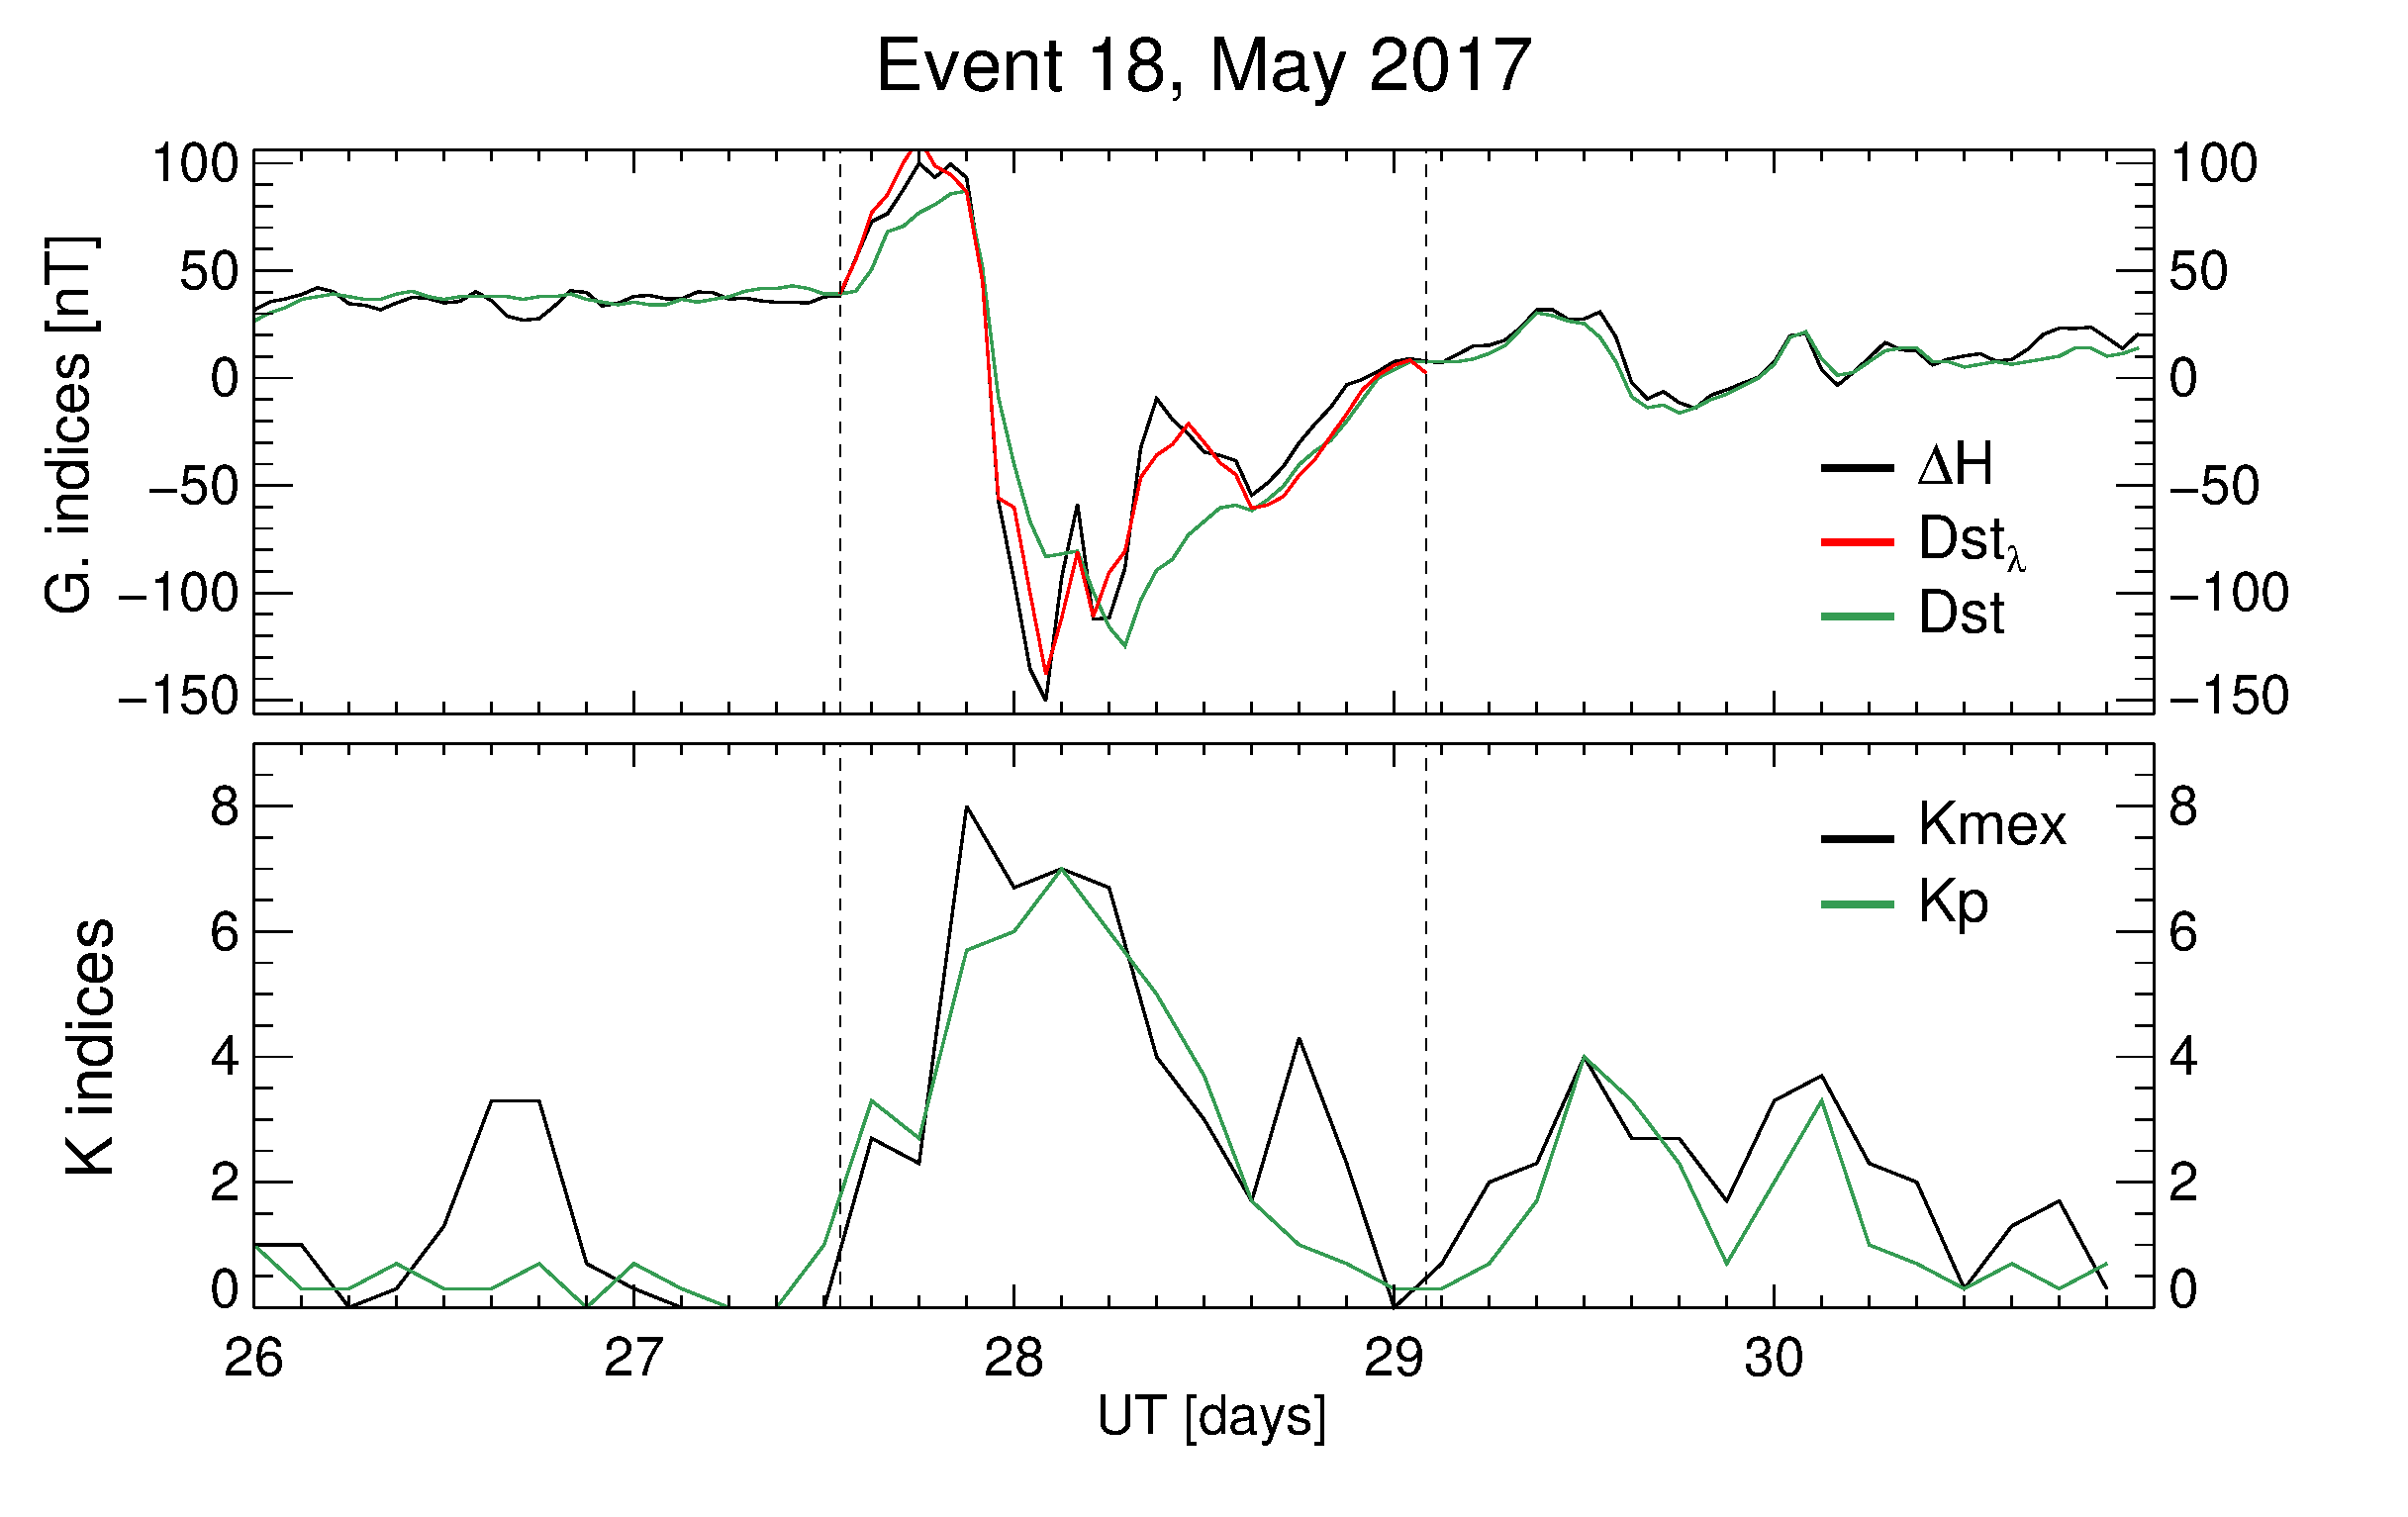
\includegraphics[width=8.0cm]{images/dH_approx/diono_valid_V4_2017-05-26.eps} 		
	
	\caption{Comparisson between regional and planetary geomagnetic response for events 3, 6, 13 and 18. Each event shows data from Dst, $\Delta$H, ${Dst_\lambda}$, ${K_P}$ and ${K_{mex}}$ indices. Planetary indices are depicted by green solid lines, while local geomagnetic indices are represented by black solid lines. The $Dst_\lambda$ index is indicated by the red line}
	\label{fig:iono_valid}
\end{figure*}


This process was repeated with all our study cases. The Figures \ref{fig:iono_valid2} and \ref{fig:iono_valid3} show the results of our validation exercise. In all the cases, we found that $Dst_\lambda$ consistently approximates $\Delta H$. We also found that $Kp$ with the combined effects of $Dst_\lambda$ was able to enclose the regional $K$ values.

Now, in addition to our previous qualitative comparisson; we proceed with a quantitative exploration. For this purpose we compute the average absolute difference between the pairs $\Delta H$-$Dst$ and $\Delta H$-$Dst_\lambda$ for our study cases. The results for this exploration are shown by Figure \ref{fig:valid}. In the figure we observe a histogram with the average difference between $\Delta H$-$Dst$ (blue bars) and $\Delta H$-$Dst_\lambda$ (red bars). We note that average difference associated with $Dst_\lambda$ is systematically lesser than that associated with $Dst$. Thus the effects of magnetic perturbations consistent with those provoked by $DP2$ and $Ddyn$ are relevant for regional geomagnetic response.

%To validate comprehensively, this process is applied to all studied cases. Figures \ref{fig:iono_valid2} and \ref{fig:iono_valid3} showcase the results. Consistently, $ Dst_\lambda$ approximates $\Delta H$, and $K_p$ with the effects of $Dst_\lambda$ encapsulates regional $K$ values.

%Additionally, a quantitative assessment is conducted. The average absolute differences between $\Delta H$-$Dst$ and $\Delta H$-$Dst_\lambda$ pairs across the study cases are computed. As displayed in Figure \ref{fig:valid}, the histogram illustrates the average differences between $\Delta H$-$Dst$ (blue bars) and $\Delta H$-$Dst_\lambda$ (red bars). Notably, the average difference associated with $Dst_\lambda$ consistently outperforms that of $Dst$, implying the relevance of magnetic perturbations corresponding to $DP2$ and $Ddyn$ for regional geomagnetic responses.

\begin{figure}
\centering
    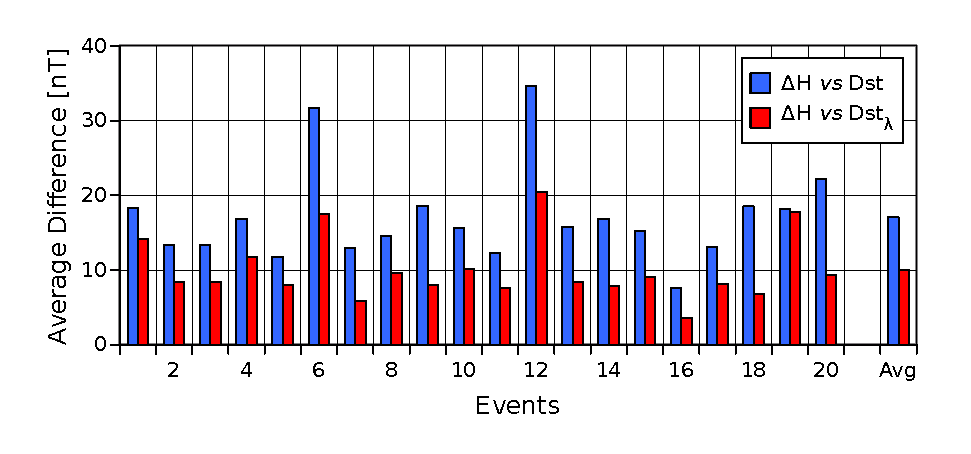
\includegraphics[width=0.5\textwidth]{images/prom_dist.eps}
    \caption{The average differnce between the planetary and regional geomagnetic response as registerd by Dst and $\Delta H$ indices for all the analyzed events. Blue bars represent the difference between $\Delta H$ and Dst, whereas red bars represent the difference between $\Delta H$ and $Dst_\lambda$ (red bars).}
    \label{fig:valid}
\end{figure}


Finally, our third and last step for our validation process is to remake the dispersion plot of Figure \ref{fig:disp}, but using $Dst_\lambda$ data instead of $Dst$'s. Figure \ref{fig:valid_disp2} shows the new dispersion plot where we can appreciate, in contrast with Figure \ref{fig:disp}, that data points (open diamonds) closely follow the identity (solid black line). Furthermore, when we compute the correlation indices we obtain note that $R^2$ grew from 0.77 up to 0.86 for the range of $Dst \ge -100\, {\rm nT}$. In addition, for the case of $Dst < -100\, {\rm nT}$, $R^2=0.75$ which is significant increment from the value originally associated to $Dst$ ($R^2=0.42$).
%The final step involves remaking the dispersion plot from Figure \ref{fig:disp}, employing $Dst_\lambda$ data instead of $Dst$. The resulting Figure \ref{fig:valid_disp2} depicts data points (open diamonds) closely following the identity (solid black line), in contrast with Figure \ref{fig:disp}. Moreover, $R^2$ improves from 0.77 to 0.86 for $Dst \ge -100\, {\rm nT}$, and for $Dst < -100\, {\rm nT}$, $R^2$ rises to 0.75, a significant increase from the original $Dst$ value ($R^2=0.42$).

      
\begin{figure}
    \centering
     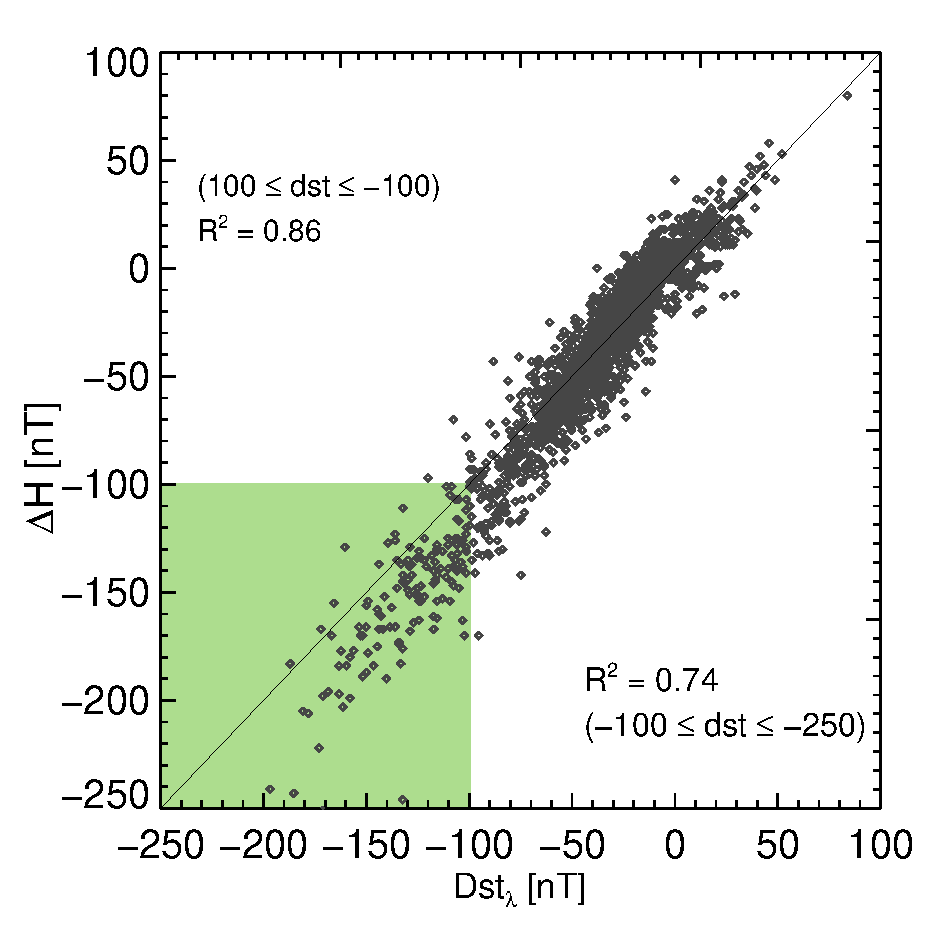
\includegraphics[width=0.45\textwidth]{dispersion_general_dst_ld.eps}
      \caption{Dispersion plot of regional response, and planetary geomagnetic response combined with local ionospheric effects. In the vertical axis we plot $\Delta H$ and in the horizontal axis we plot $Dst_\lambda$ for all anlyzed events. The figure also shows the correlation indices for data with $Dst \ge -100\, {\rm nT}$ and $-250 {\rm nT}\le Dst < -100\, {\rm nT}$ (shadowed-green region).}
       \label{fig:valid_disp2}
\end{figure}

Our validation process proved that the magnetic perturbations tentatively induced by $DP2$ and $Ddyn$ ionospheric currents, when combined with planetary indices, allowed to qualitatively approximate the regional geomagnetic activity. We also proved that regional geomagnetic response, as registered by $\Delta H$, can be quantitatively expressed by the planetary response ($Dst$) combined with the geomagnetic effects of the already commented ionospheric currents. Finally, when including the magnetic effects induced by $DP2$ and $Ddyn$ into the planetary response, the dispersion between regional and planetary data substantially decreased.


%Our validation process proved that the magnetic perturbations tentatively induced by $DP2$ and $Ddyn$ ionospheric currents, when combined with planetary indices, allowed to qualitatively approximate the regional geomagnetic activity. We also proved that regional geomagnetic response, as registered by $\Delta H$, can be quantitatively expressed by the planetary response ($Dst$) combined with the geomagnetic effects of the already commented ionospheric currents. Finally, when including the magnetic effects induced by $DP2$ and $Ddyn$ into the planetary response, the dispersion between regional and planetary data substantially decreased.

%Through this validation process, we successfully demonstrate that the magnetic perturbations potentially induced by $DP2$ and $Ddyn$ ionospheric currents, when combined with planetary indices, allow for qualitative and quantitative approximations of regional geomagnetic activity. Furthermore, the disparity between regional and planetary data is substantially reduced by integrating the magnetic effects resulting from $DP2$ and $Ddyn$ into the planetary response.



\section{Concluding remarks}

In this work we studied the regional manifestations of space weather at central Mexico. We focused on the differences between planetary and local geomagnetic responses during periods of strong geomagnetic storms ($GS$). We also investigated the possible sources for such differences in the geomagnetic response. In order to do so, we used the geomagnetic registers from the Teoloyucan Magnetic Observatory (TEO), located at north of Mexico City. We also use data sets from the $Dst$ and $K_P$ planetary indices, as well as the regional geomagnetic index $\Delta H$ and the total electron content delivered by the Mexican Space Weather National Laboratory (\href{http://regmex.unam.mx}{REGMEX/LANCE}).

We selected 20 $GS$ as study cases for this work (see Table \ref{table1:GS_descp}). We identified evidence for the presence of relevant regional geomagnetic response through a dispersion plot (see Figure \ref{fig:disp}). In this regard, we found that in the range of $Dst < -100 {\rm nT}$ there is a tendency for the regional geomagnetic index to deviate from the planetary one. We assumed this as an evidence for regional geomagnetic response.

Subsequently, we isolated the geomagnetic effects due to ionospheric processes ($D_I$) from the regional (TEO) geomagnetic registers. Next, we applied filters on $D_I$ with the purpose of identify the magnetic perturbations consistent with those induce by $Ddyn$ and $DP2$ currents. We also verified that intensification of the resulting $Ddyn$ and $DP2$ profiles simultaneously occurred during $TEC$ perturbations (see discussion of Figure \ref{fig:iono_resp}). In consequence, we were able to reconstruct the regional geomagnetic response consistent with those induced by $Ddyn$ and $DP2$ currents.

Afterwards, we validate our computed geomagnetic contribution due to $Ddyn$ and $DP2$ currents. First, we approximate the regional $K$ and $\Delta H$ indices by combining the planetary $K_P$ and $Dst$ indices with the regional geomagnetic effects of $Ddyn$ and $DP2$. Secondly, we computed the differences between $\Delta H$ and $Dst$ with and without the regional ionospheric effects. Finally, we analyzed the dispersion between $\Delta H$ and $Dst$ combined with the effects of $Ddyn$ and $DP2$. For all the cases, we found that regional geomagnetic response is qualitatively and quantitatively approximated by the geomagnetic planetary response combined with the geomagnetic perturbations induced by the $Ddyn$ and $DP2$ ionospheric currents. 

%Finally, in this work we focus on regional space weather. We identified evidence of regional geomagnetic response that is significantly different from its planetary counterpart. We investigated $Ddyn$ and $DP2$ ionospheric currents as the mechanisms for such a regional response. As a result, we were able to isolate the magnetic perturbations associated with those ionospheric currents. The combination of these perturbations with planetary response could approximate the regional geomagnetic response.


%In this work we focus on regional space weather in Central Mexico by studying local geomagnetic and ionospheric data. We identified evidence of regional geomagnetic response that is significantly different from its planetary counterpart. We investigated $Ddyn$ and $DP2$ ionospheric currents as possible mechanisms for such a regional response. As a result, we were able to isolate the magnetic perturbations associated with those ionospheric currents, which is consistent with the local ionospheric TEC response. The combination of these perturbations with planetary response succeeded in approximate the regional geomagnetic response, i.e. the regional geomagnetic response has a significant component from local ionospheric effects.

Thus, our study shows that regional space-weather manifestations at central Mexico may significantly deviate from the planetary response. In consequence, in order to address the regional effects of, and risks due to, space-weather in Central Mexico, it is necessary to carry out studies from a regional approach, complemented with the planetary context. Our results highlight the particularities that geomagnetic response has for a given location. Hence, in order to achieve a better understanding of space weather and to improve the operational response, our results evidence for the necessity to include more registers (magnetometers) into the computing of geomagnetic indices, whether planetary or regional.

Hence, according to our results, during intense geomagnetic storms, in central Mexico, the effects of $Ddyn$ and $DP2$ may induce alterations in the F region of the ionosphere and displace the equatorial ionospheric anomaly towards central and southern regions of Mexico \citep[as showed by][]{dramaria_13}. Therefore we could expect these phenomena lead to ionospheric scintillation, which degrades satellite communications, as well as the precision of navigation and positioning systems, among other services. All these effects can potentially be addressed through local perturbations of the $TEC$ during geomagnetic storm periods (refer to panels (e) of Figure \ref{fig:iono_resp}).



%Our work has two relevant limitations. The first is related to the data sources available for our study and the size of the study region. Because there was only a single source of geomagnetic registers, the validity region of our study is significantly small when compared to the surface of Mexico. Therefore, the validity of our results has, in practical terms, almost a punctual nature. While the second limitation is related to the contextualization of our results with respect to other regions with similar geomagnetic latitudes/longitudes. It is important to note that both limitations are already being addressed. The first one through the development of instrumentation by LANCE, and address the last one is our immediate future work.

It is important to remark that the surface of Mexico is near 2 million ${\rm km}^2$. This fact made of our results valid only for the central region of Mexico (few thousands of ${\rm km}^2$), leaving the rest of its surface to address. In addition, Mexico is located at North America, and the ionospheric currents pass through and evolve along the whole American continent. Hence, on one hand, it is required more sources of geomagnetic registers in Mexico and, on the other hand, it is necessary to contextualize the geomagnetic response of Mexico with those present in Northern and Central America, and even South America. For the first case, LANCE is developing a the Network of Geomagnetic Stations Mexico (REGMEX) \citep[see][]{corona2024}, to monitoring regional geomagnetic response all over Mexico. Whereas, for the case of contextualize the geomagnetic response of Mexico, this is our immediate future work.

\printcredits
\section*{Declaration of competing interest}
\label{Declaration}
The authors declare that they have no known competing financial interests or personal relationships that could have appeared to
influence the work reported in this paper.
%\section*{Funding}
%\label{funding}
%This research did not receive any specific grant from funding agencies in the public, commercial, or not-for-profit sectors.
\section*{Data Availability}
\label{data_A}
Data will be made available on request.
\section*{Acknowledgments}
P. Corona-Romero is grateful for Investigadores por Mexico-CONAHCYT (CONAHCYT Research Fellow) project 1045 Space Weather Service, financed by “Consejo Nacional de Ciencia y Tecnologia” (CONAHCYT), which partially supported this work. C.I. Castellanos-Velazco is grateful for “La Beca de Posgrado en Mexico” granted by CONAHCYT. LANCE ackowledges partial financial support from CONHACyT-AEM grant 2017-01-292684, CONAHCyT LN-315829, and PAPIIT IN116023.

This work used data from the Teoloyucan Magnetic Observatory operated by the Magnetic Service of the Geophysics Institute at National and Autonomous University of Mexico (UNAM). Total electron content ($TEC$) and the geomagnetic indices $\Delta H$ and $K$, the regional counterparts of $Dst$ and $K_P$ indices respectively, are produced by the Geomagnetic Stations Network of Mexico (\href{http://regmex.unam.mx}{REGMEX}) by the Mexican Space Weather National Laboratory (LANCE), Geophysics Institute at National and Autonomous University of Mexico (UNAM).

The results presented in this paper rely on ${K_{P}}$ and ${Dst}$ geomagnetic indices calculated by the \href{https://www.gfz-potsdam.de/en/kp-index}{Helmholtz-Zentrum Potsdam Deutsches GeoForschungsZentrum Adolf-Schmidt-Observatorium} and the \href{https://wdc.kugi.kyoto-u.ac.jp/}{World Data Center for Geomagnetism, Kyoto}, respectively, from data collected at magnetic observatories. We thank the involved national institutes, the \href{https://intermagnet.github.io/}{INTERMAGNET network} and \href{https://isgi.unistra.fr}{ISGI}.

All authors have seen and approved the final version of the manuscript.  


\label{Ack}
%% Loading bibliography style file
%\bibliographystyle{model1-num-names}
\bibliographystyle{cas-model2-names}

% Loading bibliography database
\bibliography{ref_article.bib}

% Biography
\bio{}
% Here goes the biography details.
\endbio
%\bio{pic1}
% Here goes the biography details.
%\endbio

\appendix 
\section{Analysis and Results}
\label{apend}
\begin{figure*}[h!]
    \centering
    \centerline{\Large \bf   
      %\hspace{0.18\textwidth}  \color{black}{\Large{Res}}
       %\hspace{0.28\textwidth}  \color{black}{\Large{Res+TC}}
         \hfill}
          \centerline{\Large \bf   
      \hspace{0.26\textwidth}  \color{black}{}
       \hspace{0.31\textwidth}  \color{black}{}
         \hfill}
     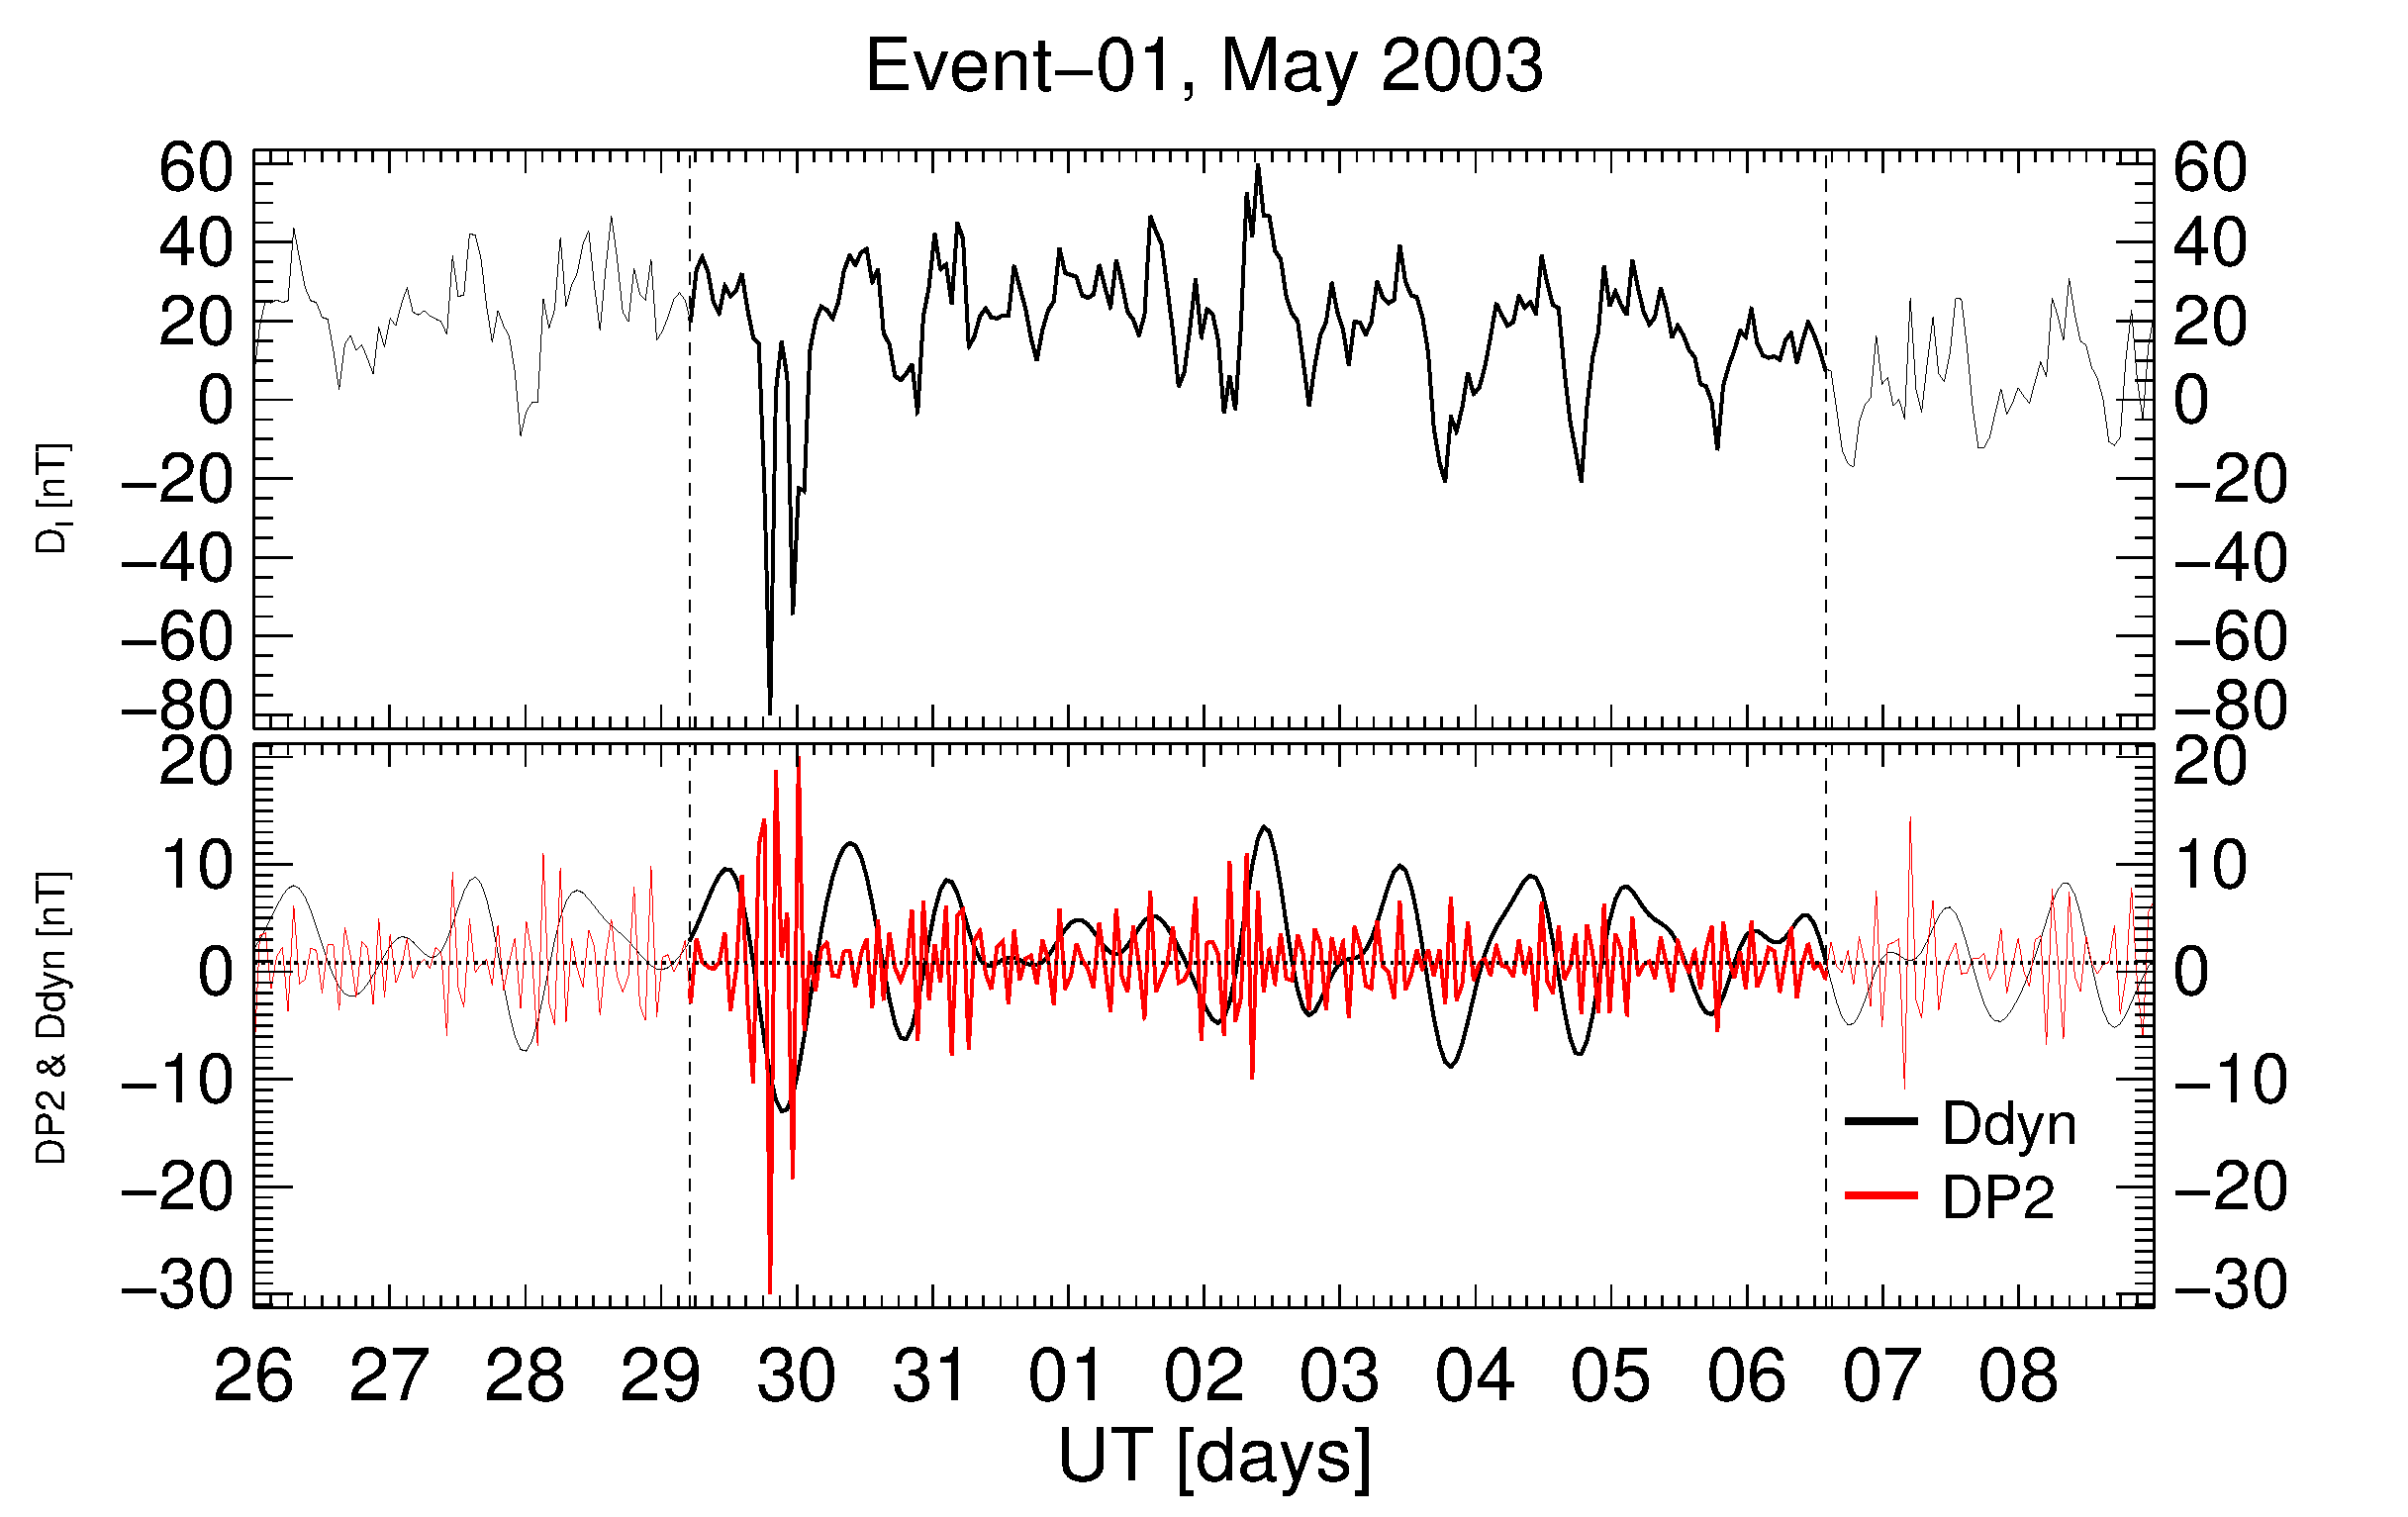
\includegraphics[width=6.0cm]{images/diono/iono_PI_V1_2003-05-26.eps}
	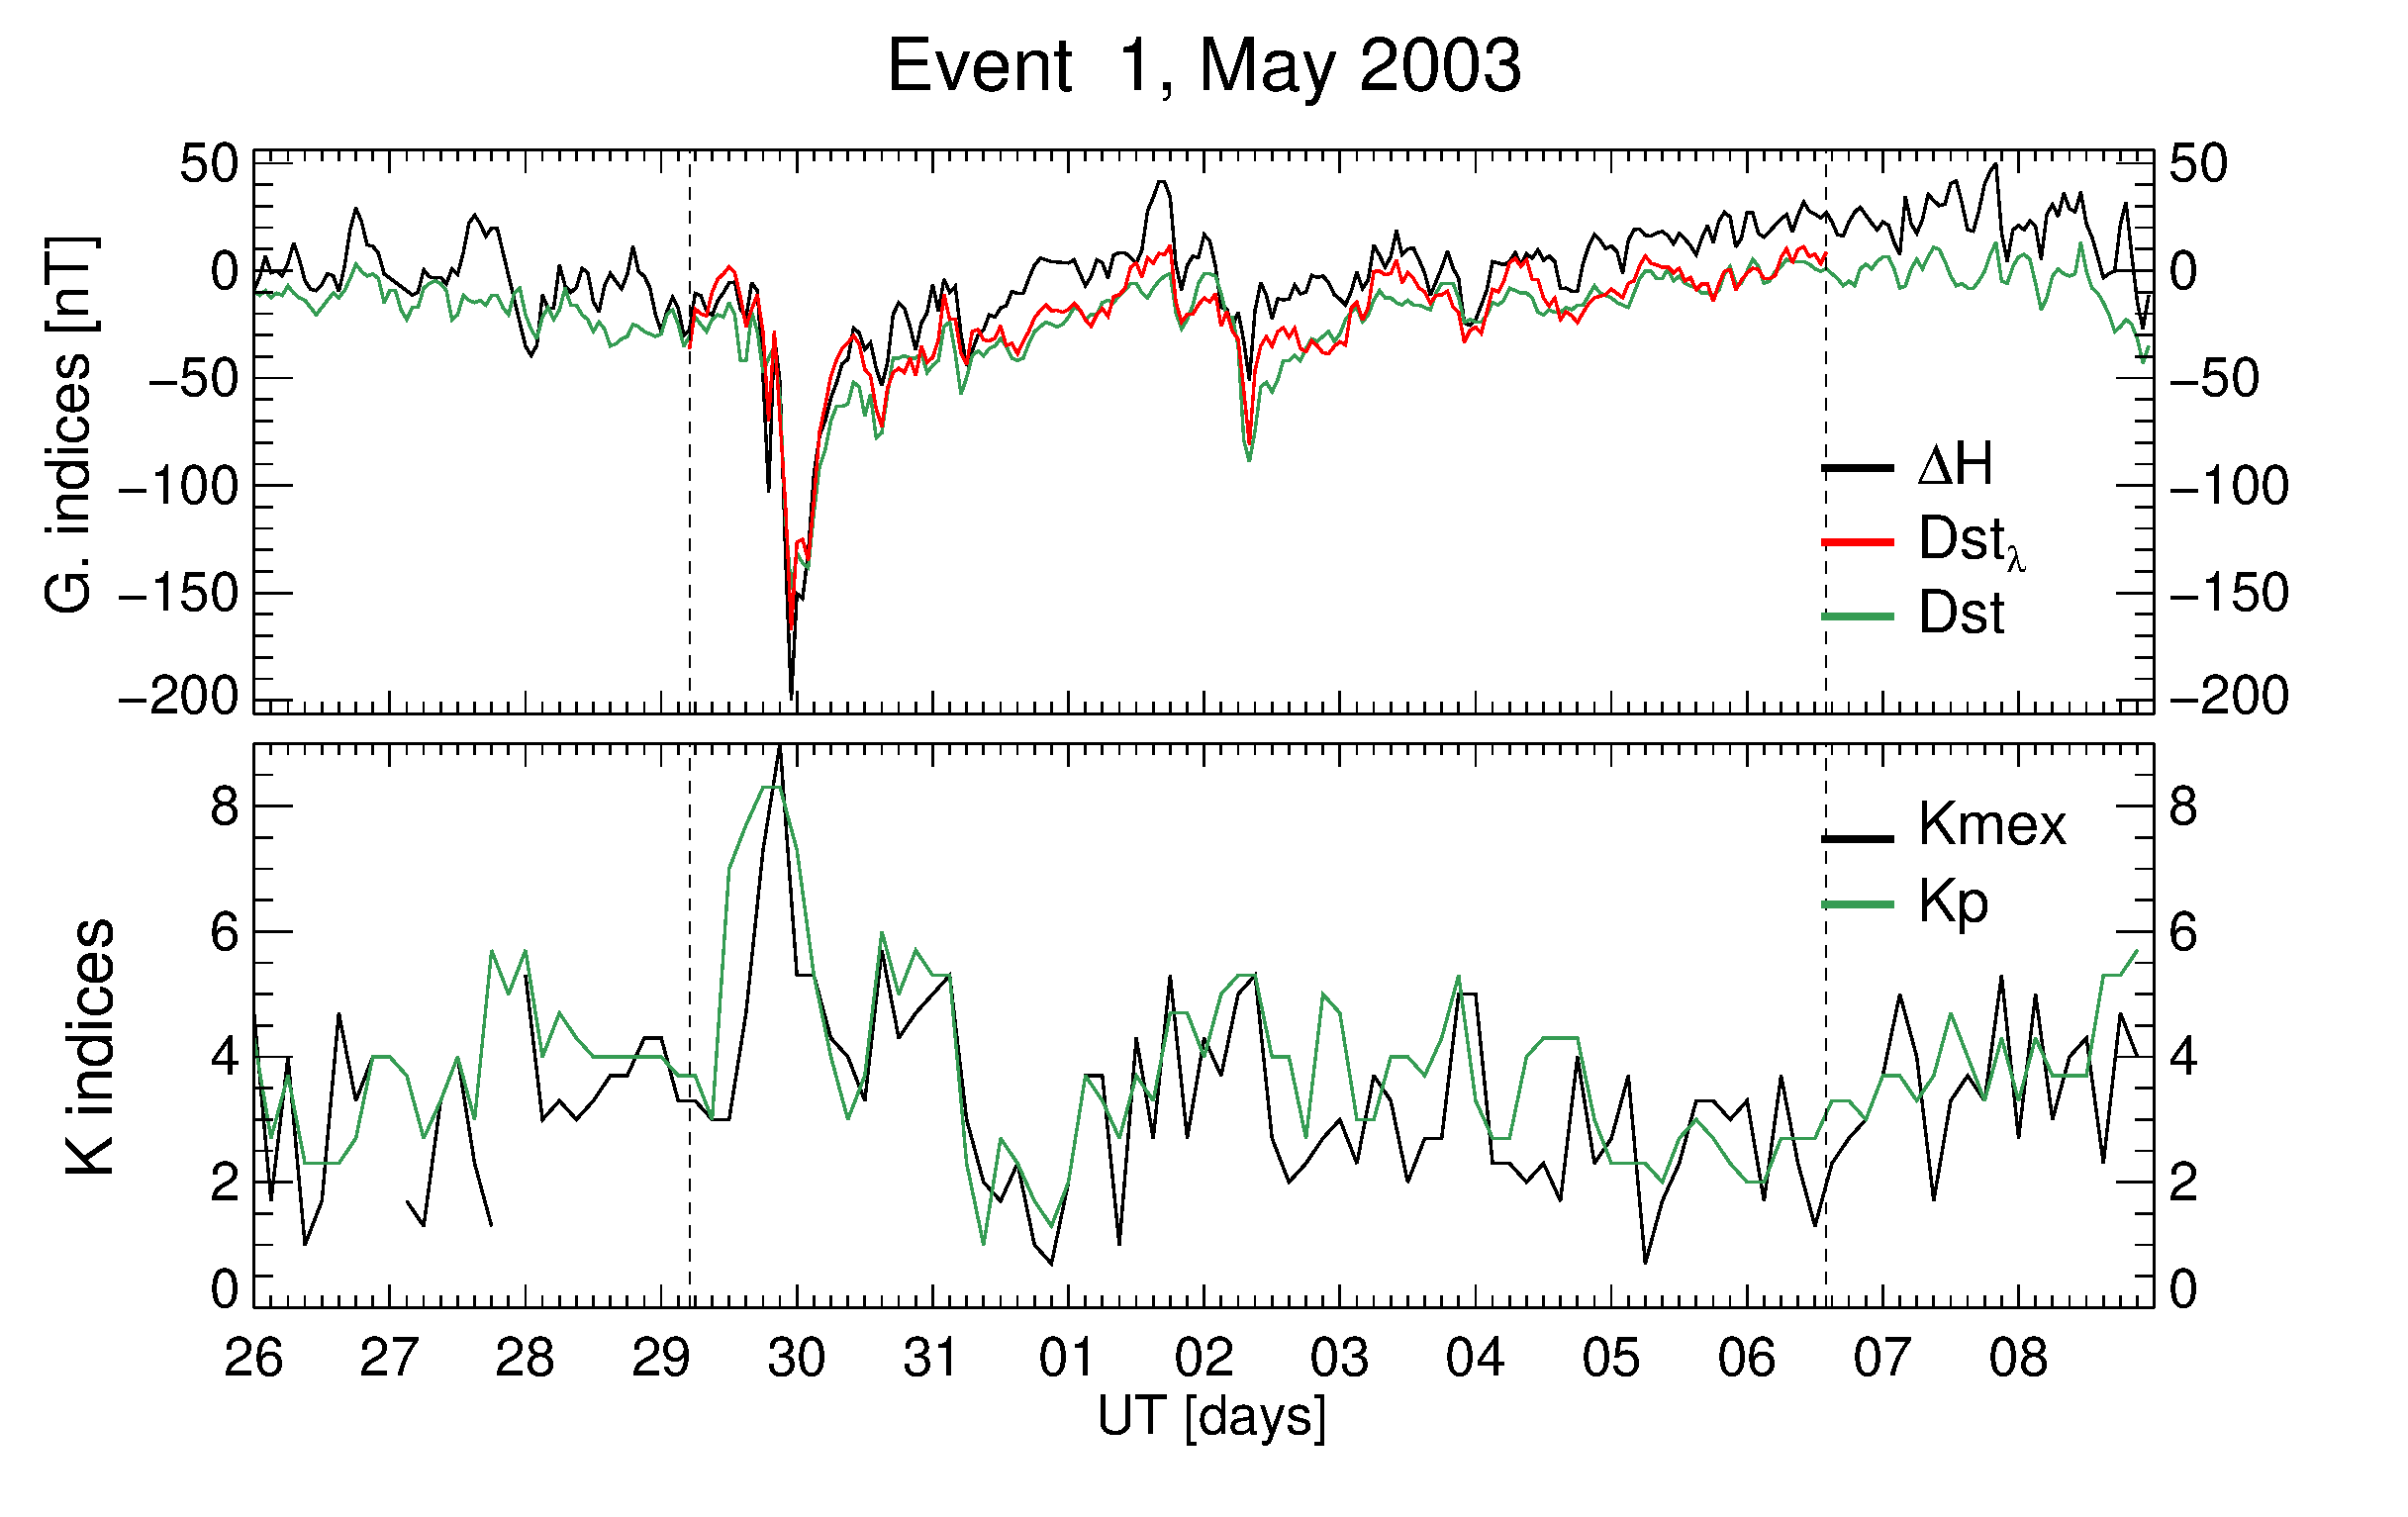
\includegraphics[width=6.0cm]{images/dH_approx/diono_valid_V4_2003-05-26.eps}
     \centerline{\Large \bf   
      \hspace{0.275\textwidth}  \color{black}{}
       \hspace{0.295\textwidth}  \color{black}{}
         \hfill}
     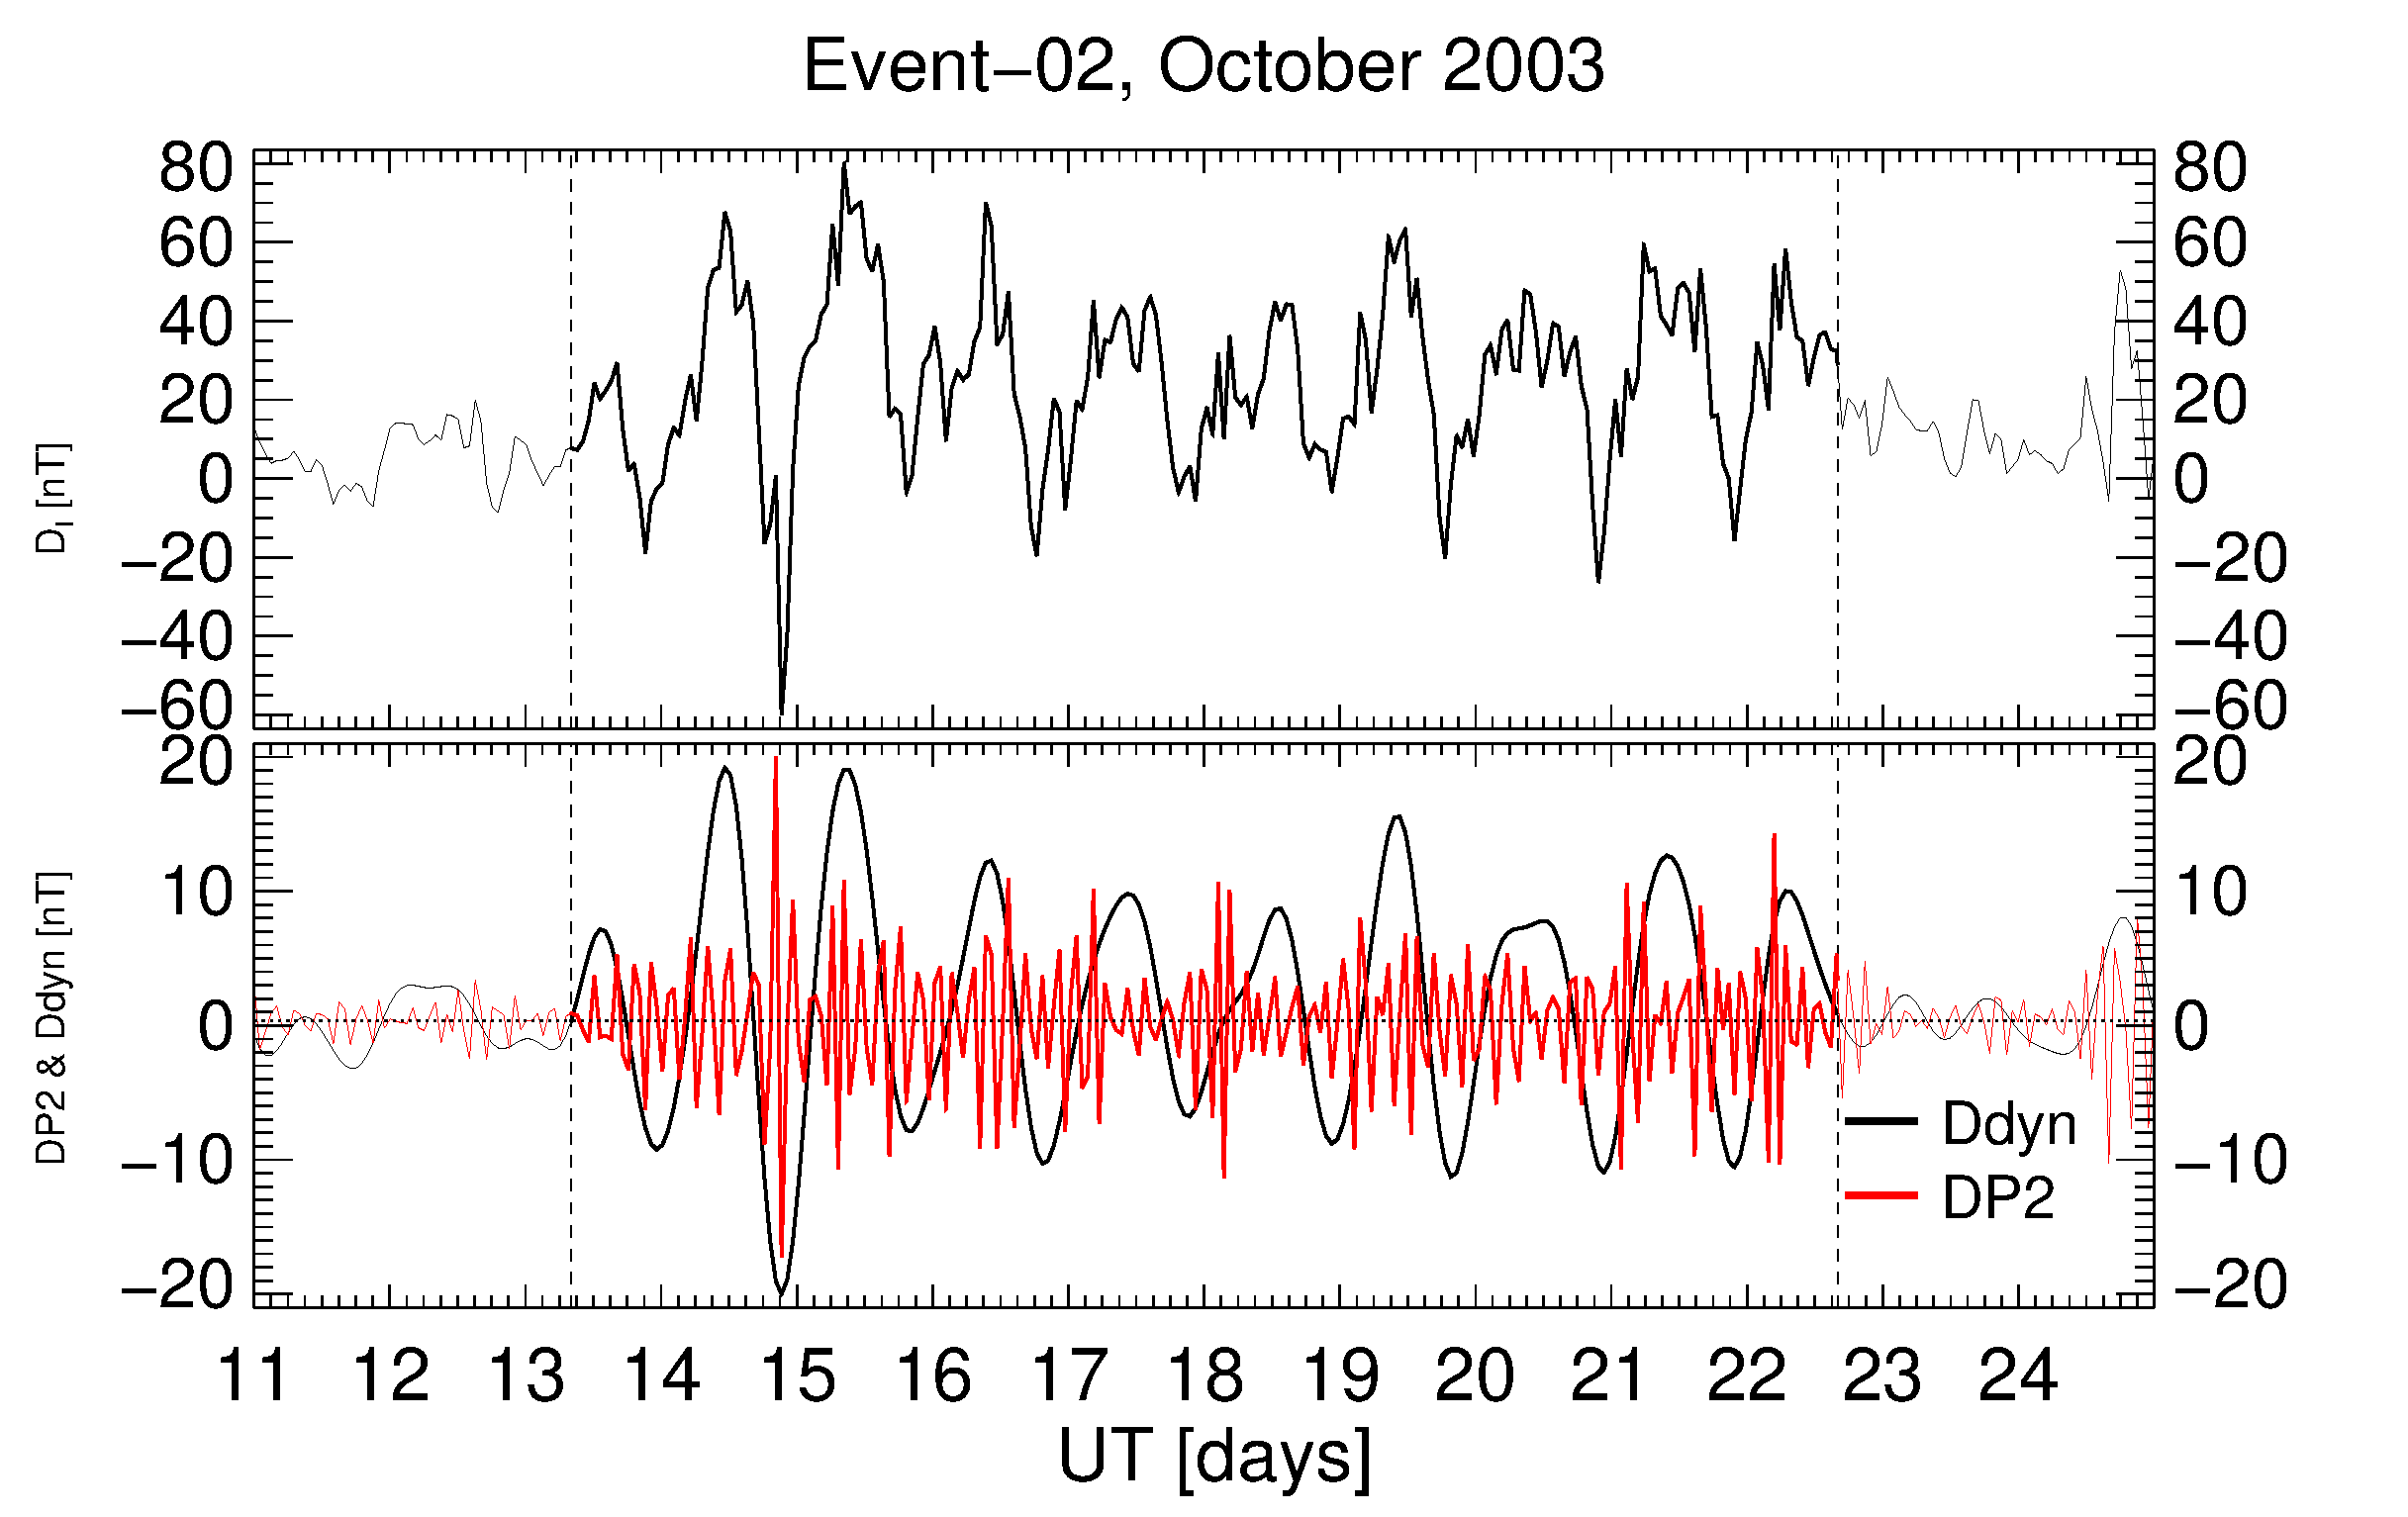
\includegraphics[width=6.0cm]{images/diono/iono_PI_V1_2003-10-11.eps}
   	 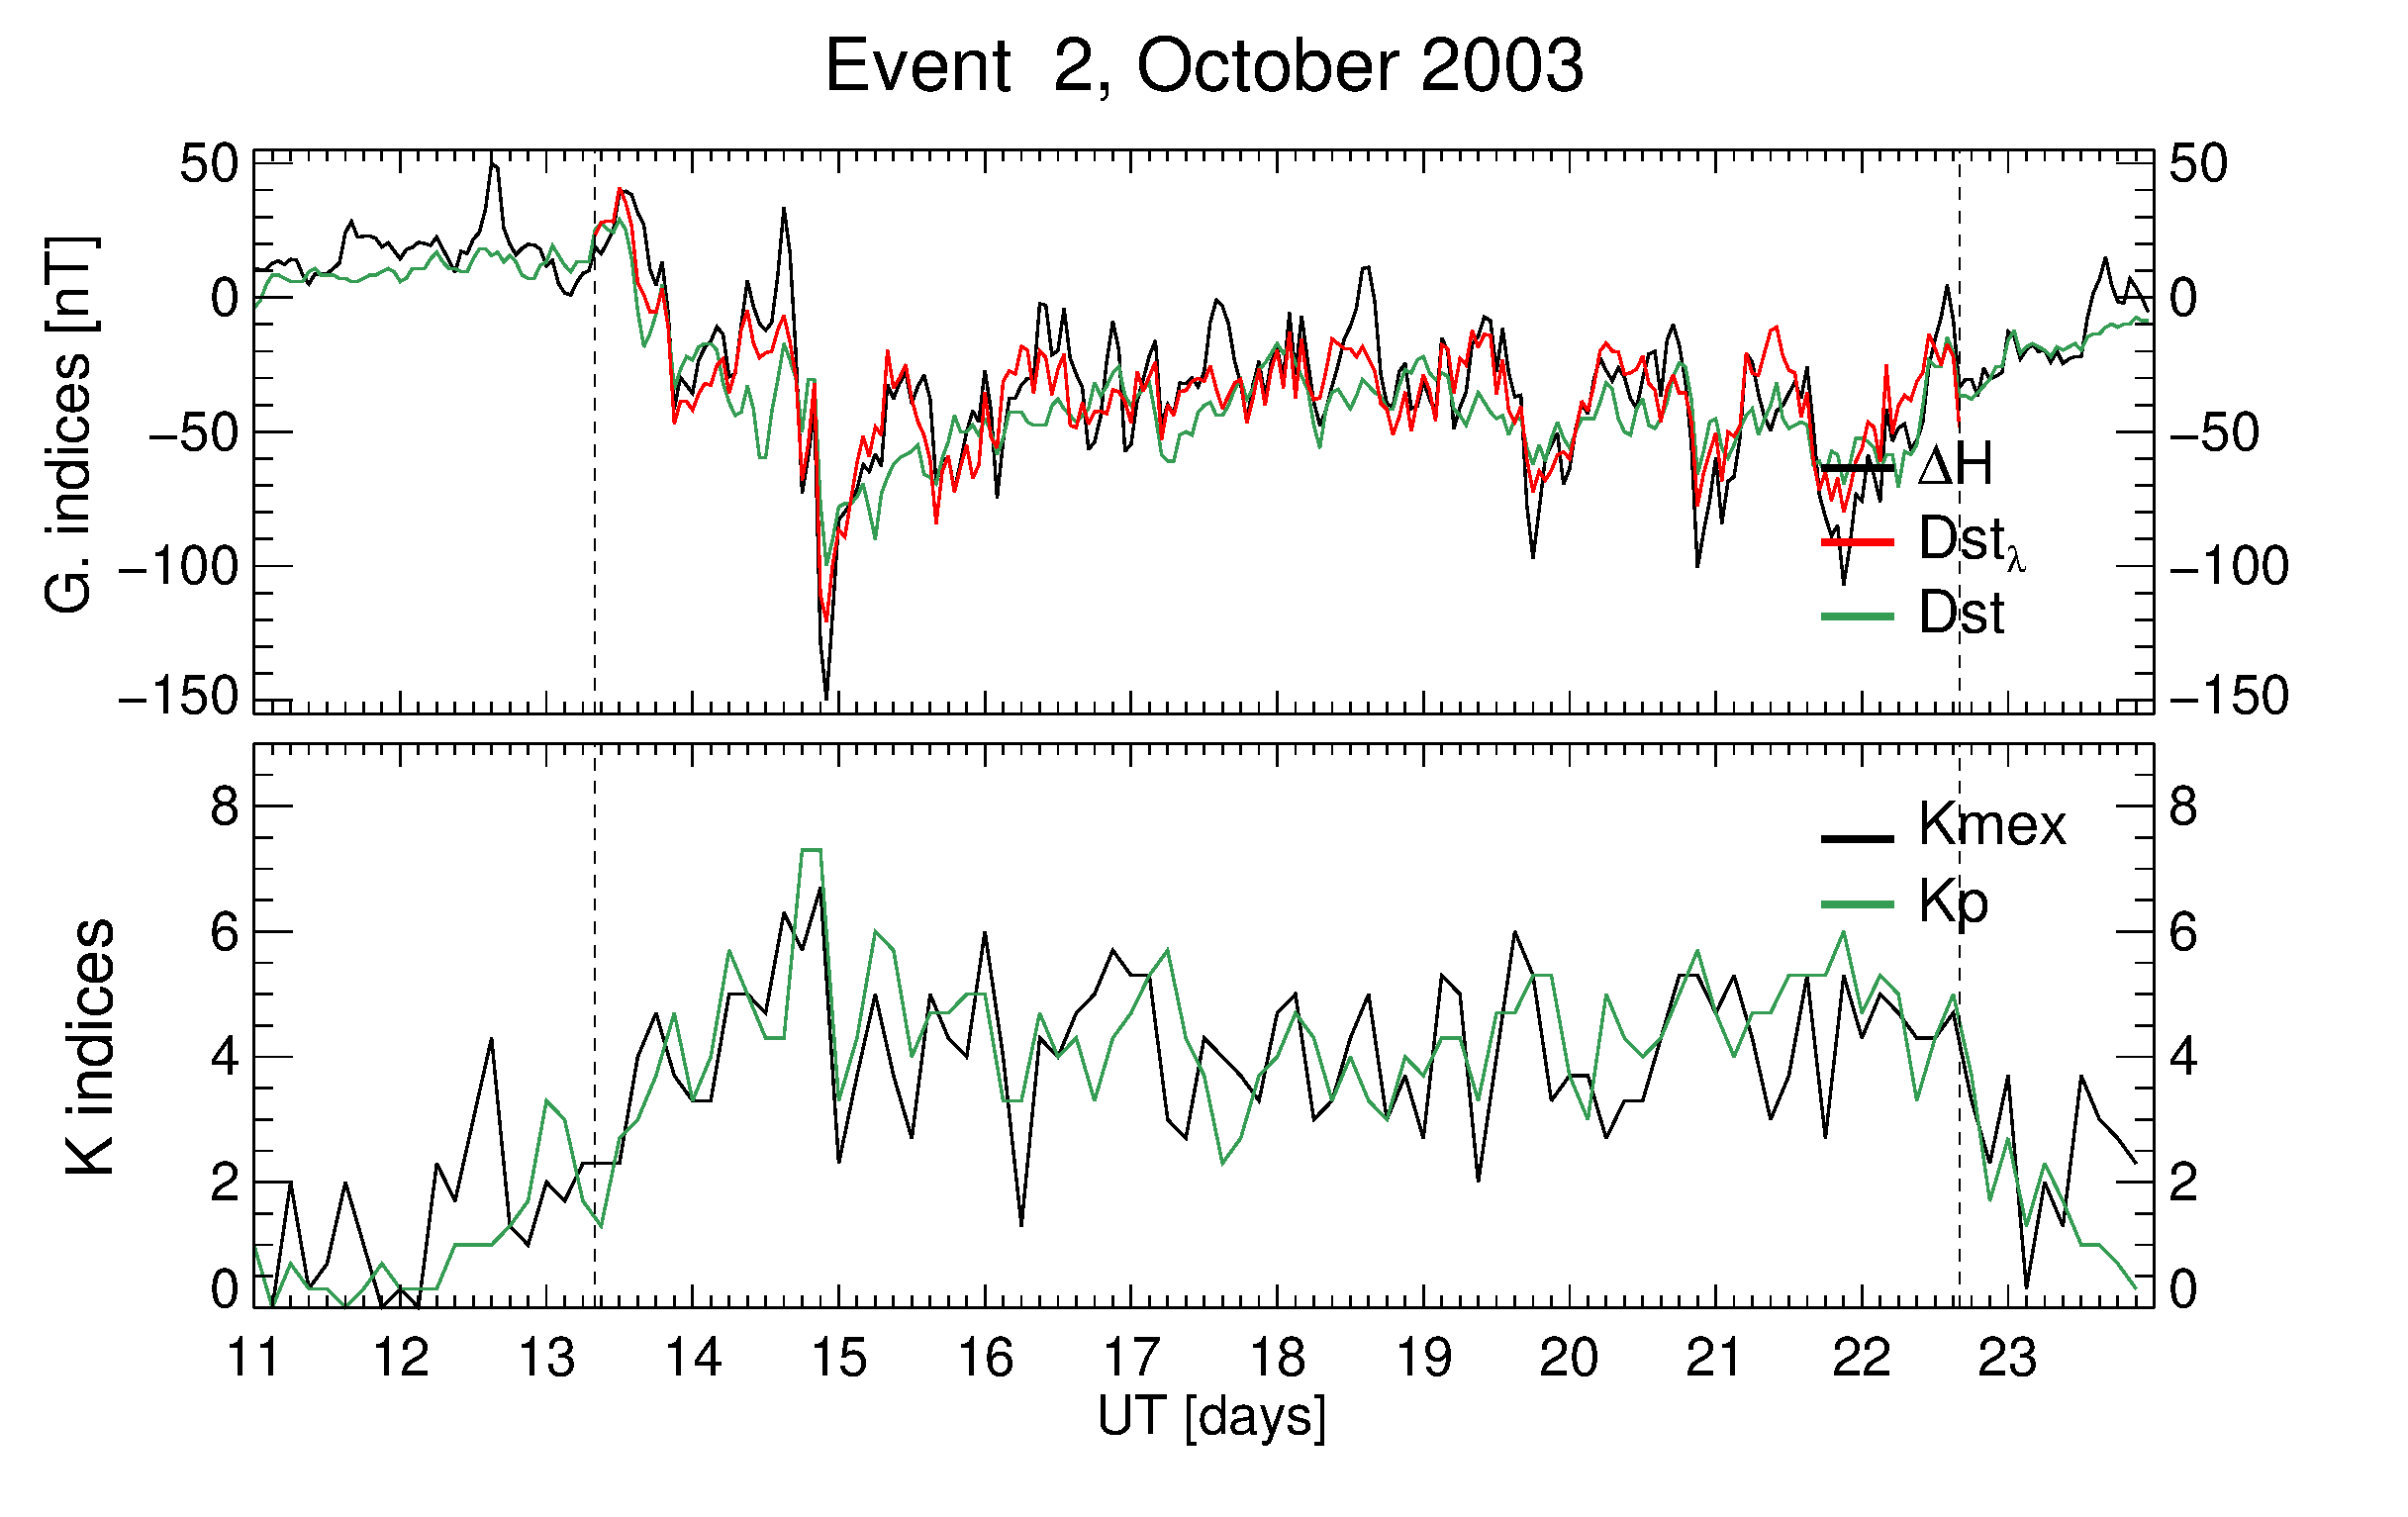
\includegraphics[width=6.0cm]{images/dH_approx/diono_valid_V4_2003-10-11.eps}
     \centerline{\Large \bf   
      \hspace{0.275\textwidth}  \color{black}{}
       \hspace{0.295\textwidth}  \color{black}{}
         \hfill}
    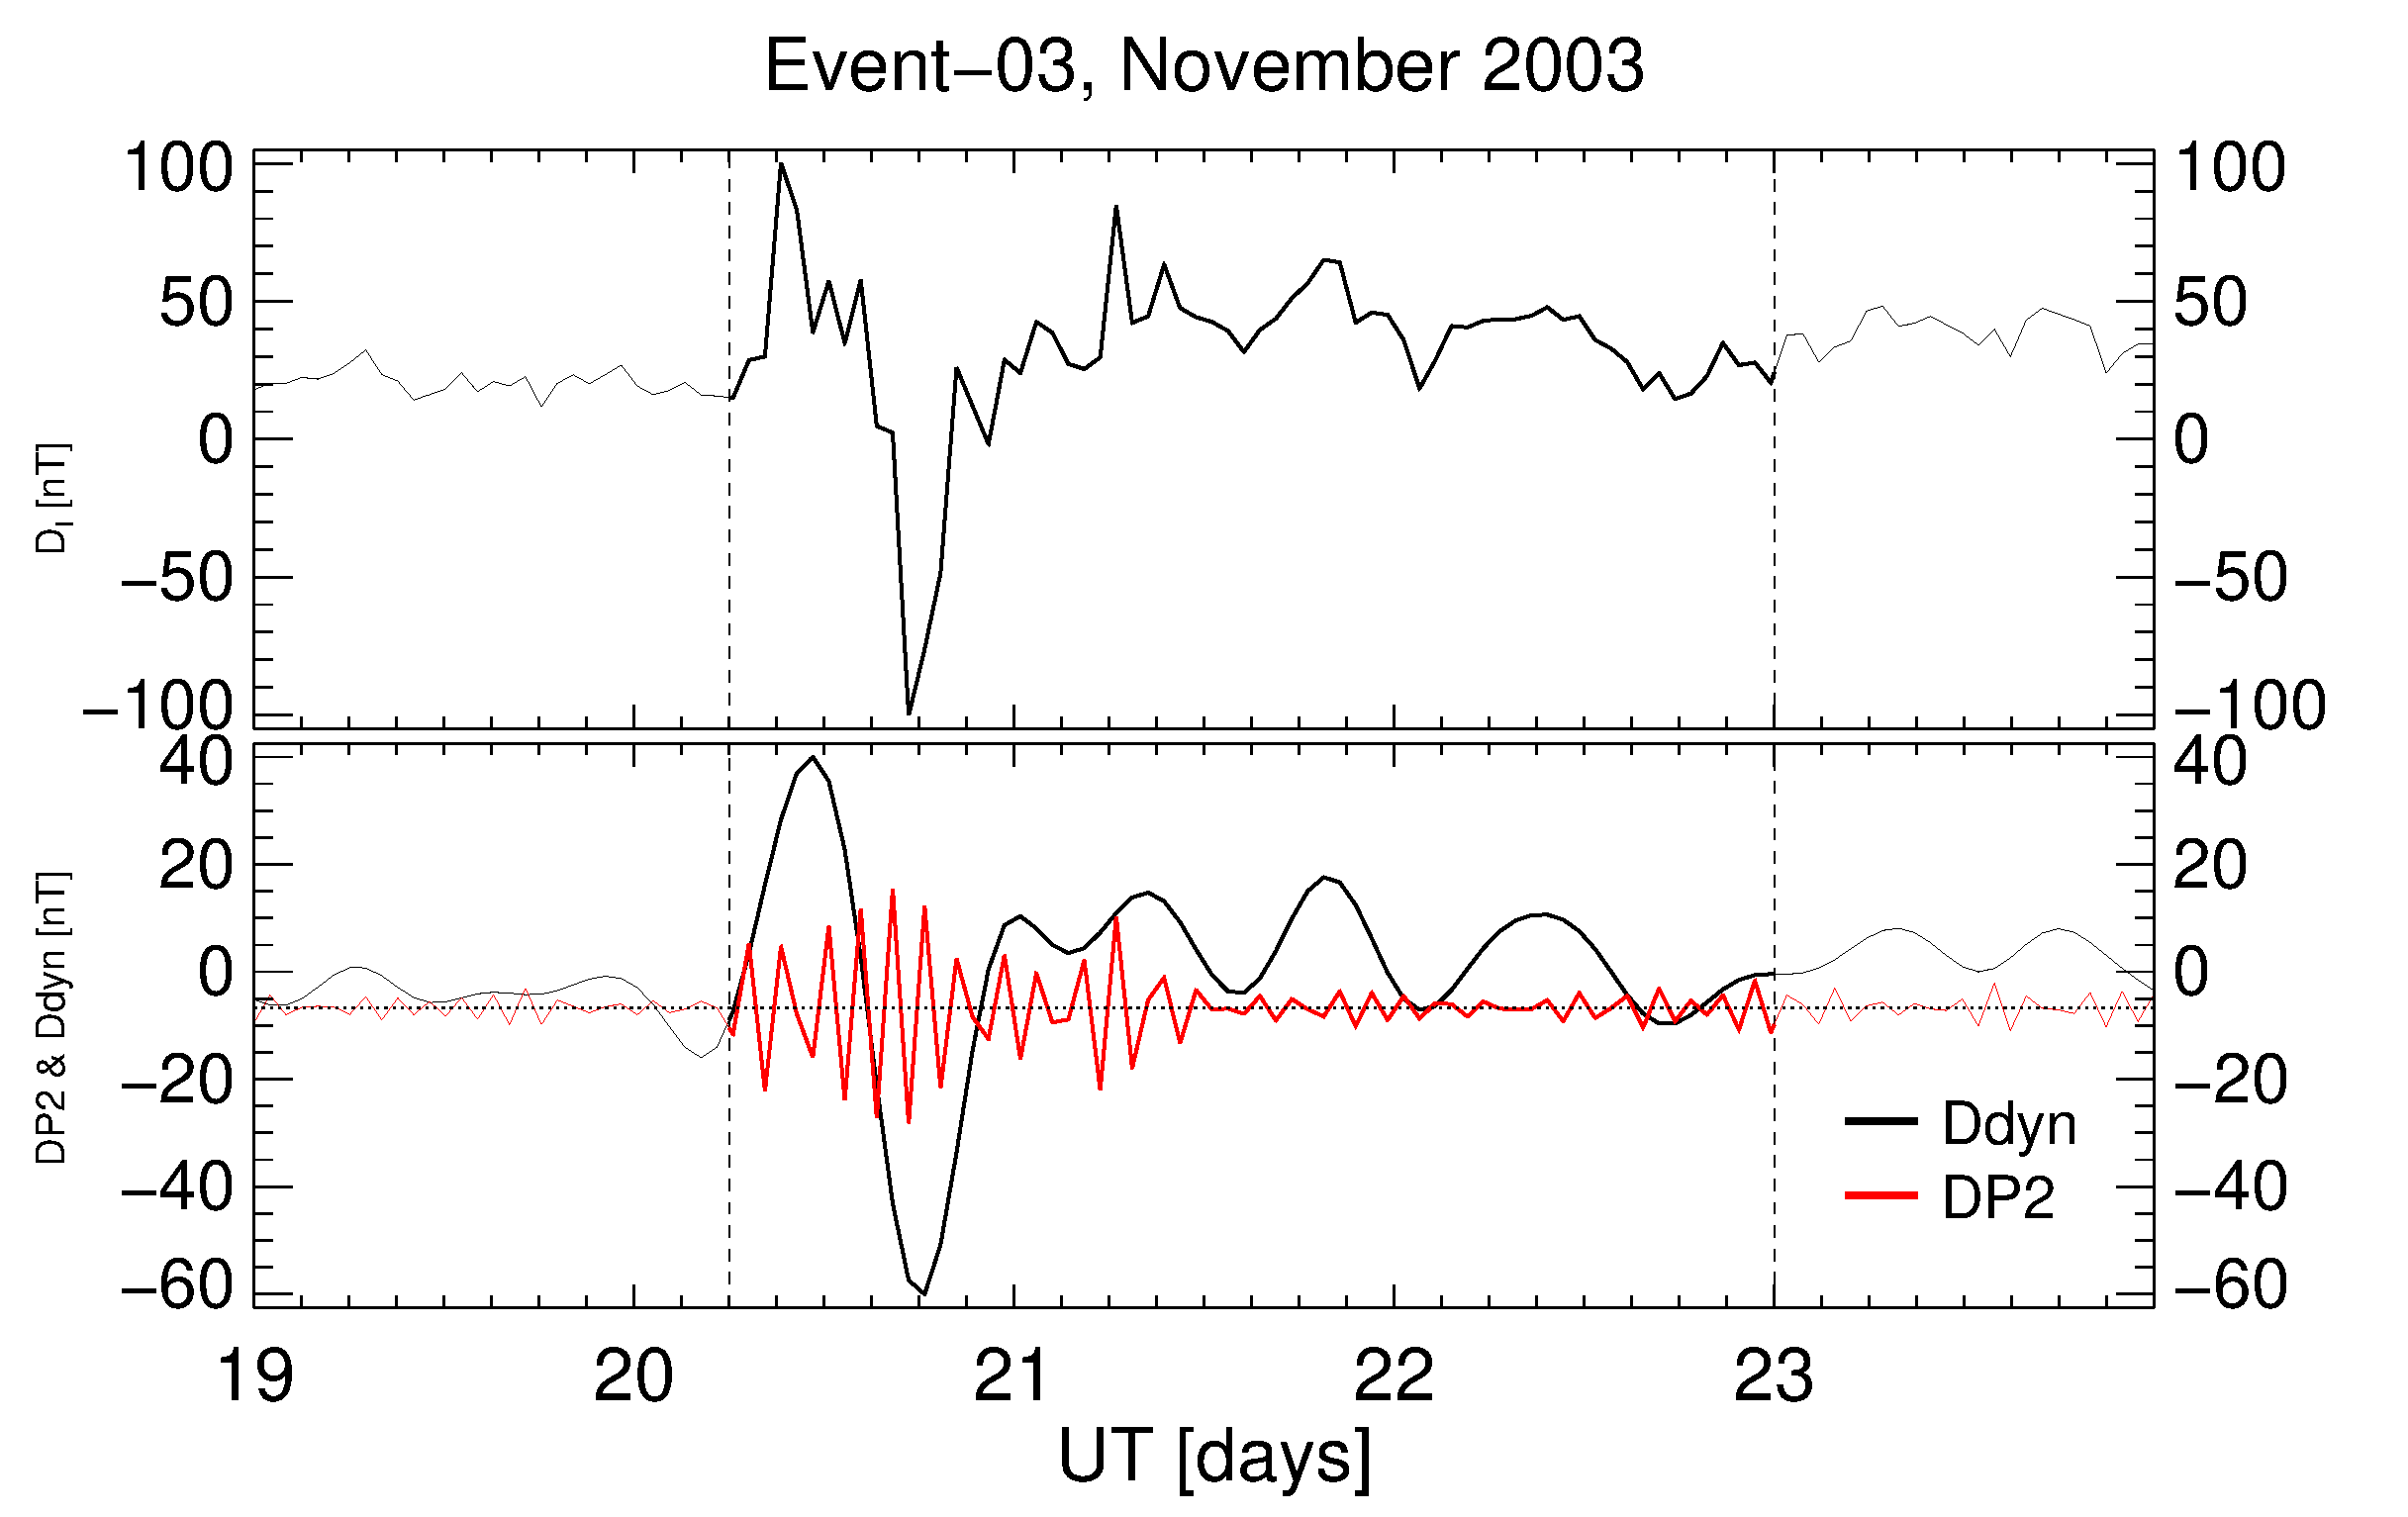
\includegraphics[width=6.0cm]{images/diono/iono_PI_V1_2003-11-19.eps} 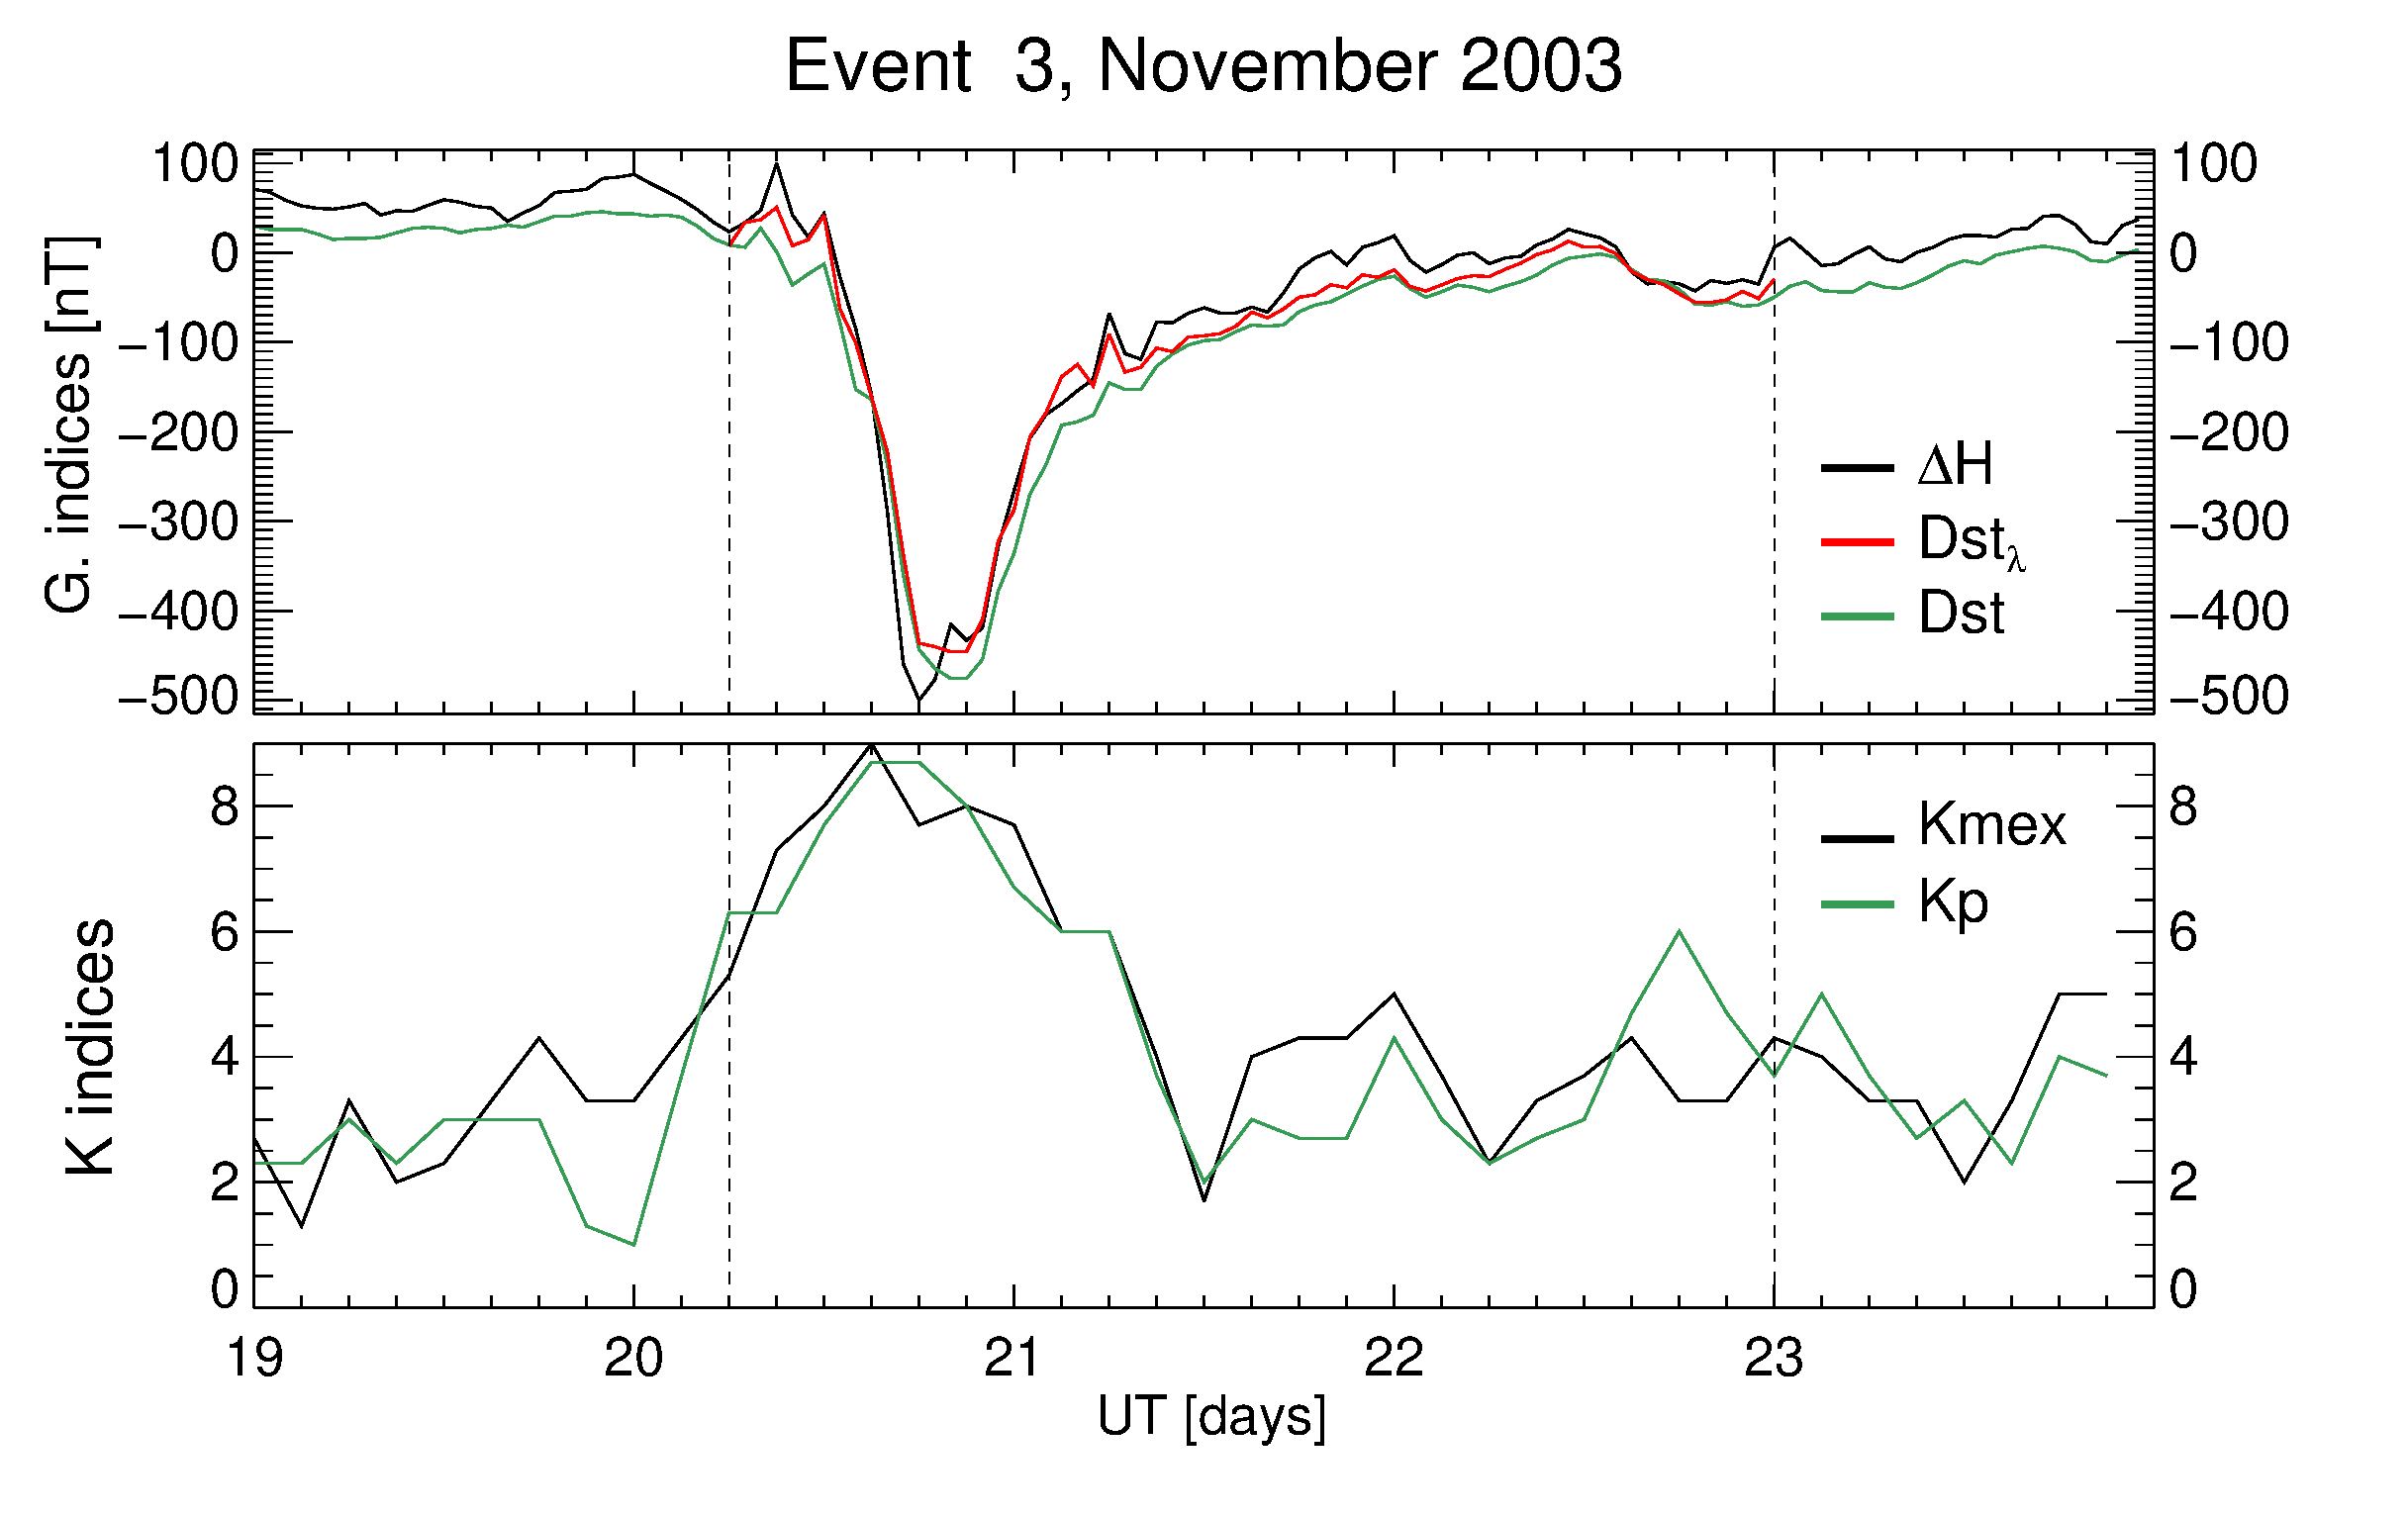
\includegraphics[width=6.0cm]{images/dH_approx/diono_valid_V4_2003-11-19.eps}            
       \centerline{\Large \bf   
      \hspace{0.275\textwidth}  \color{black}{}
       \hspace{0.295\textwidth}  \color{black}{}
         \hfill}
	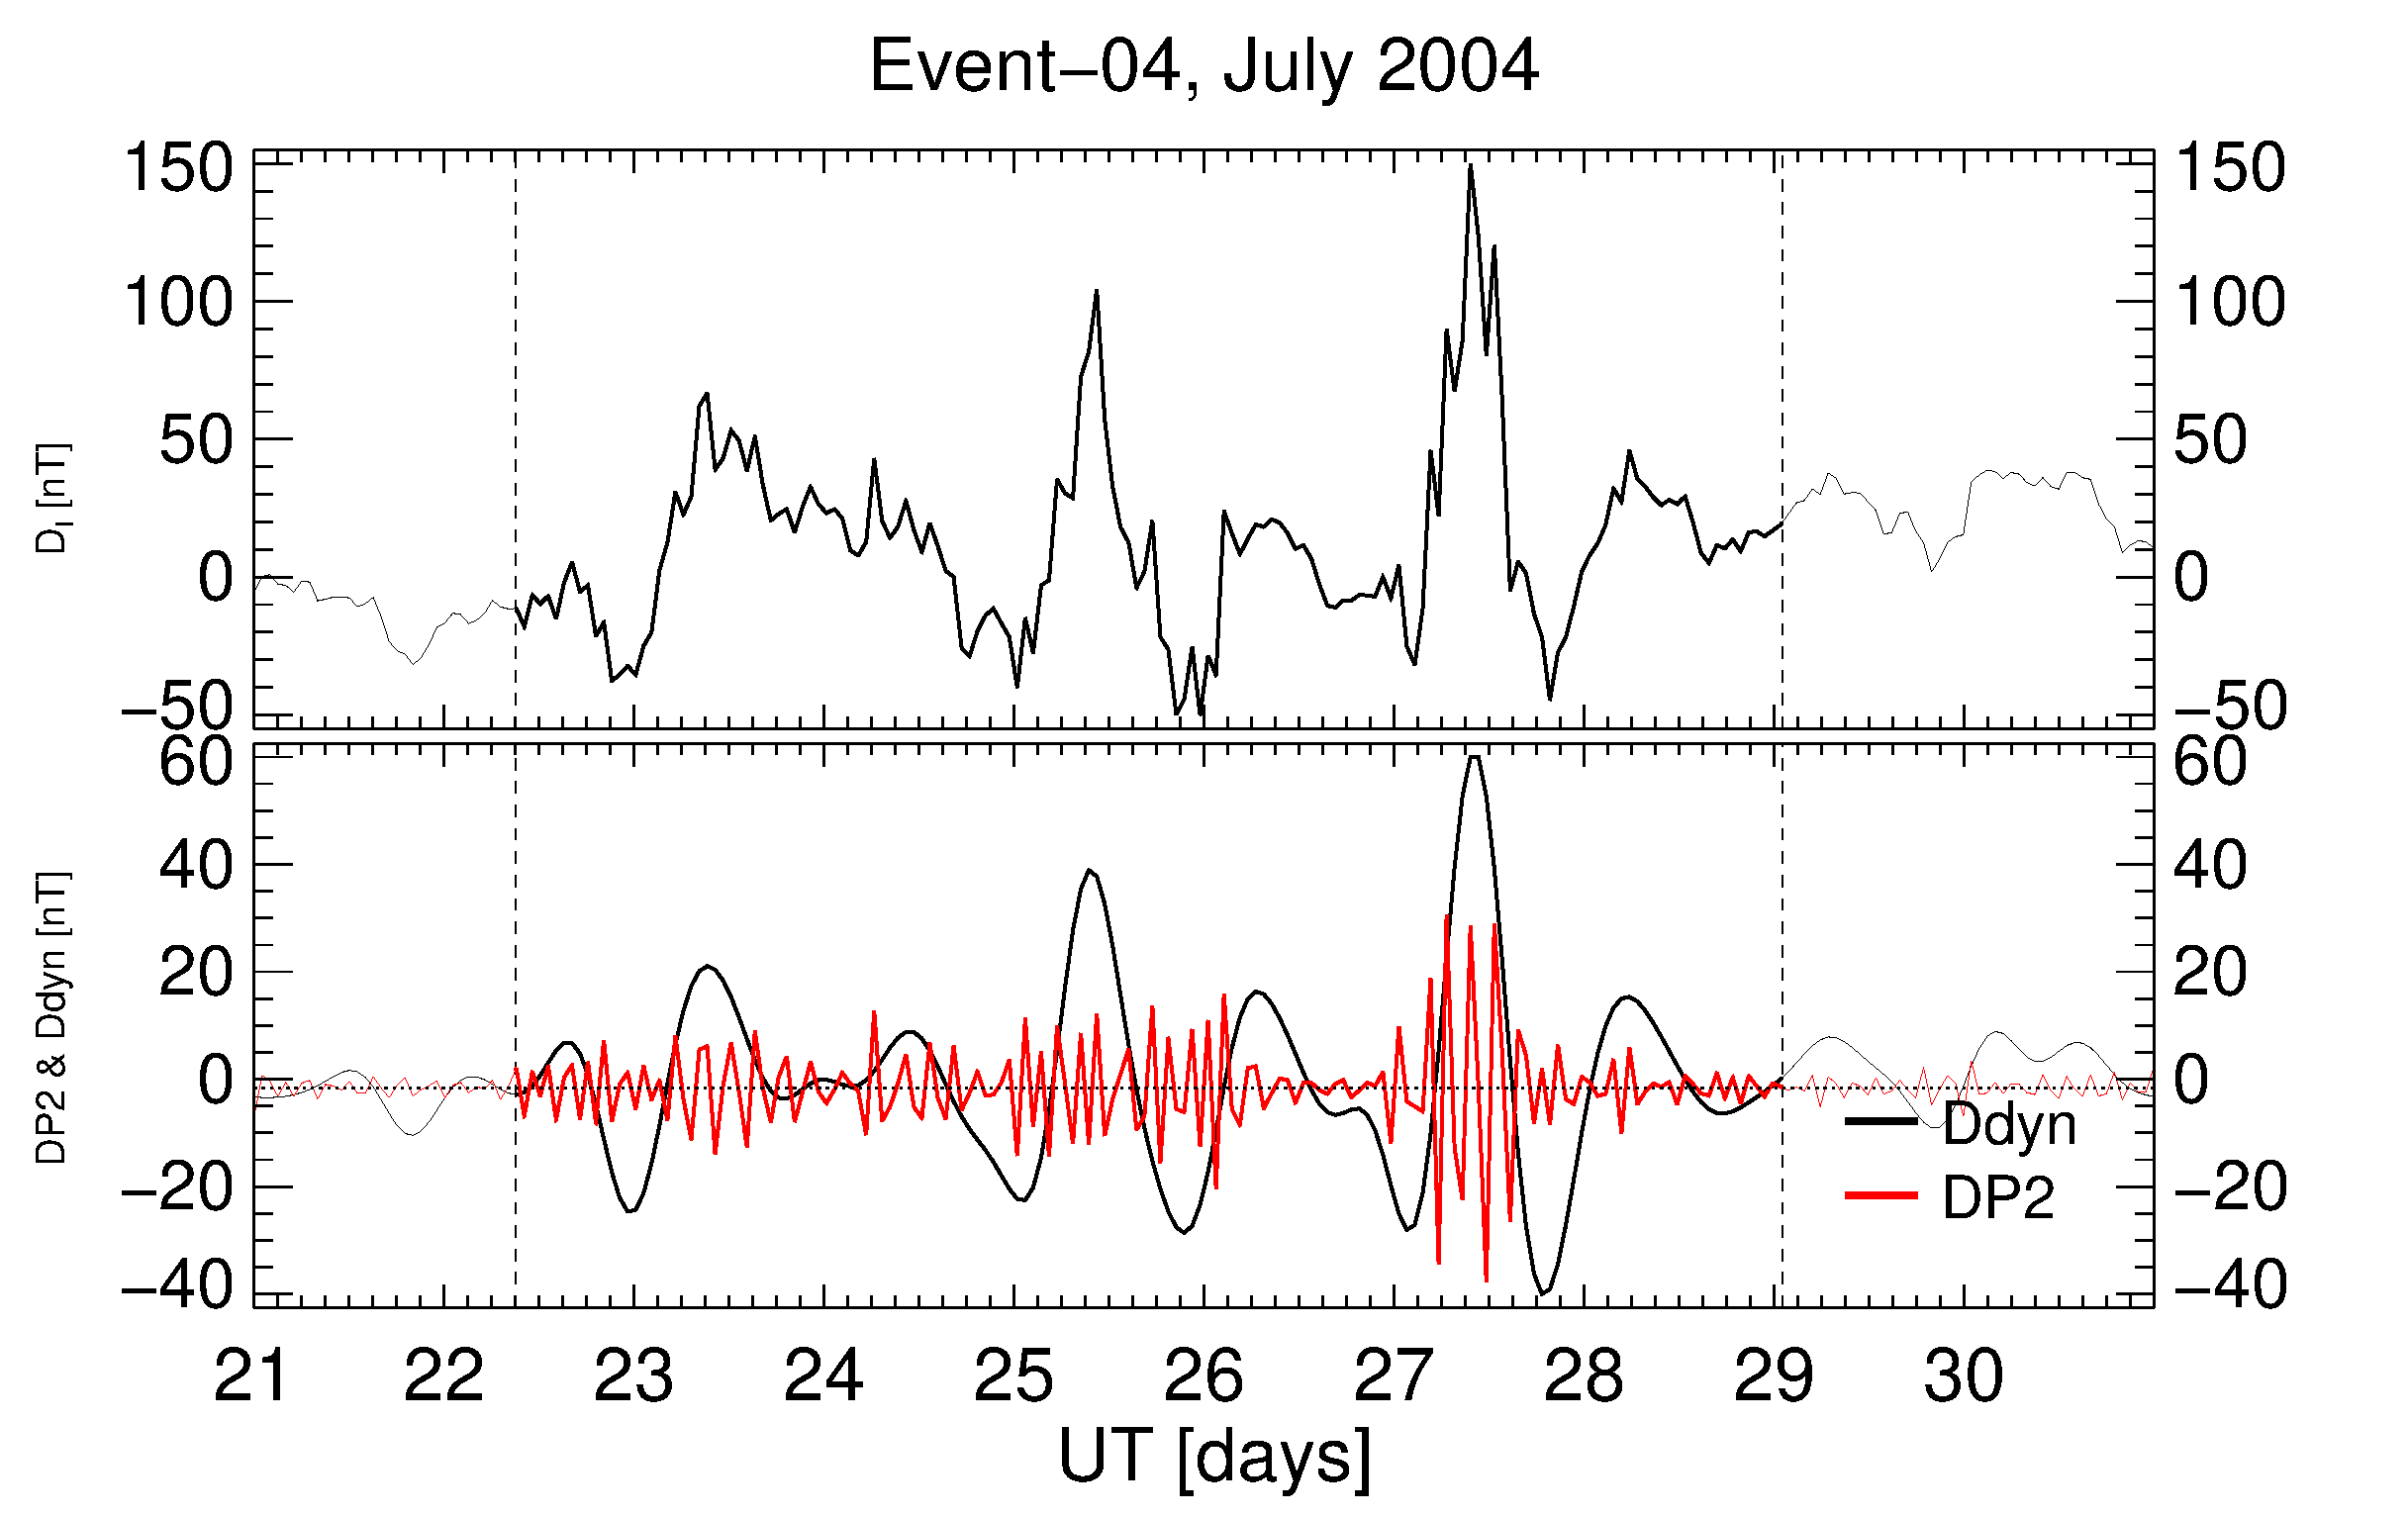
\includegraphics[width=6.0cm]{images/diono/iono_PI_V1_2004-07-21.eps}     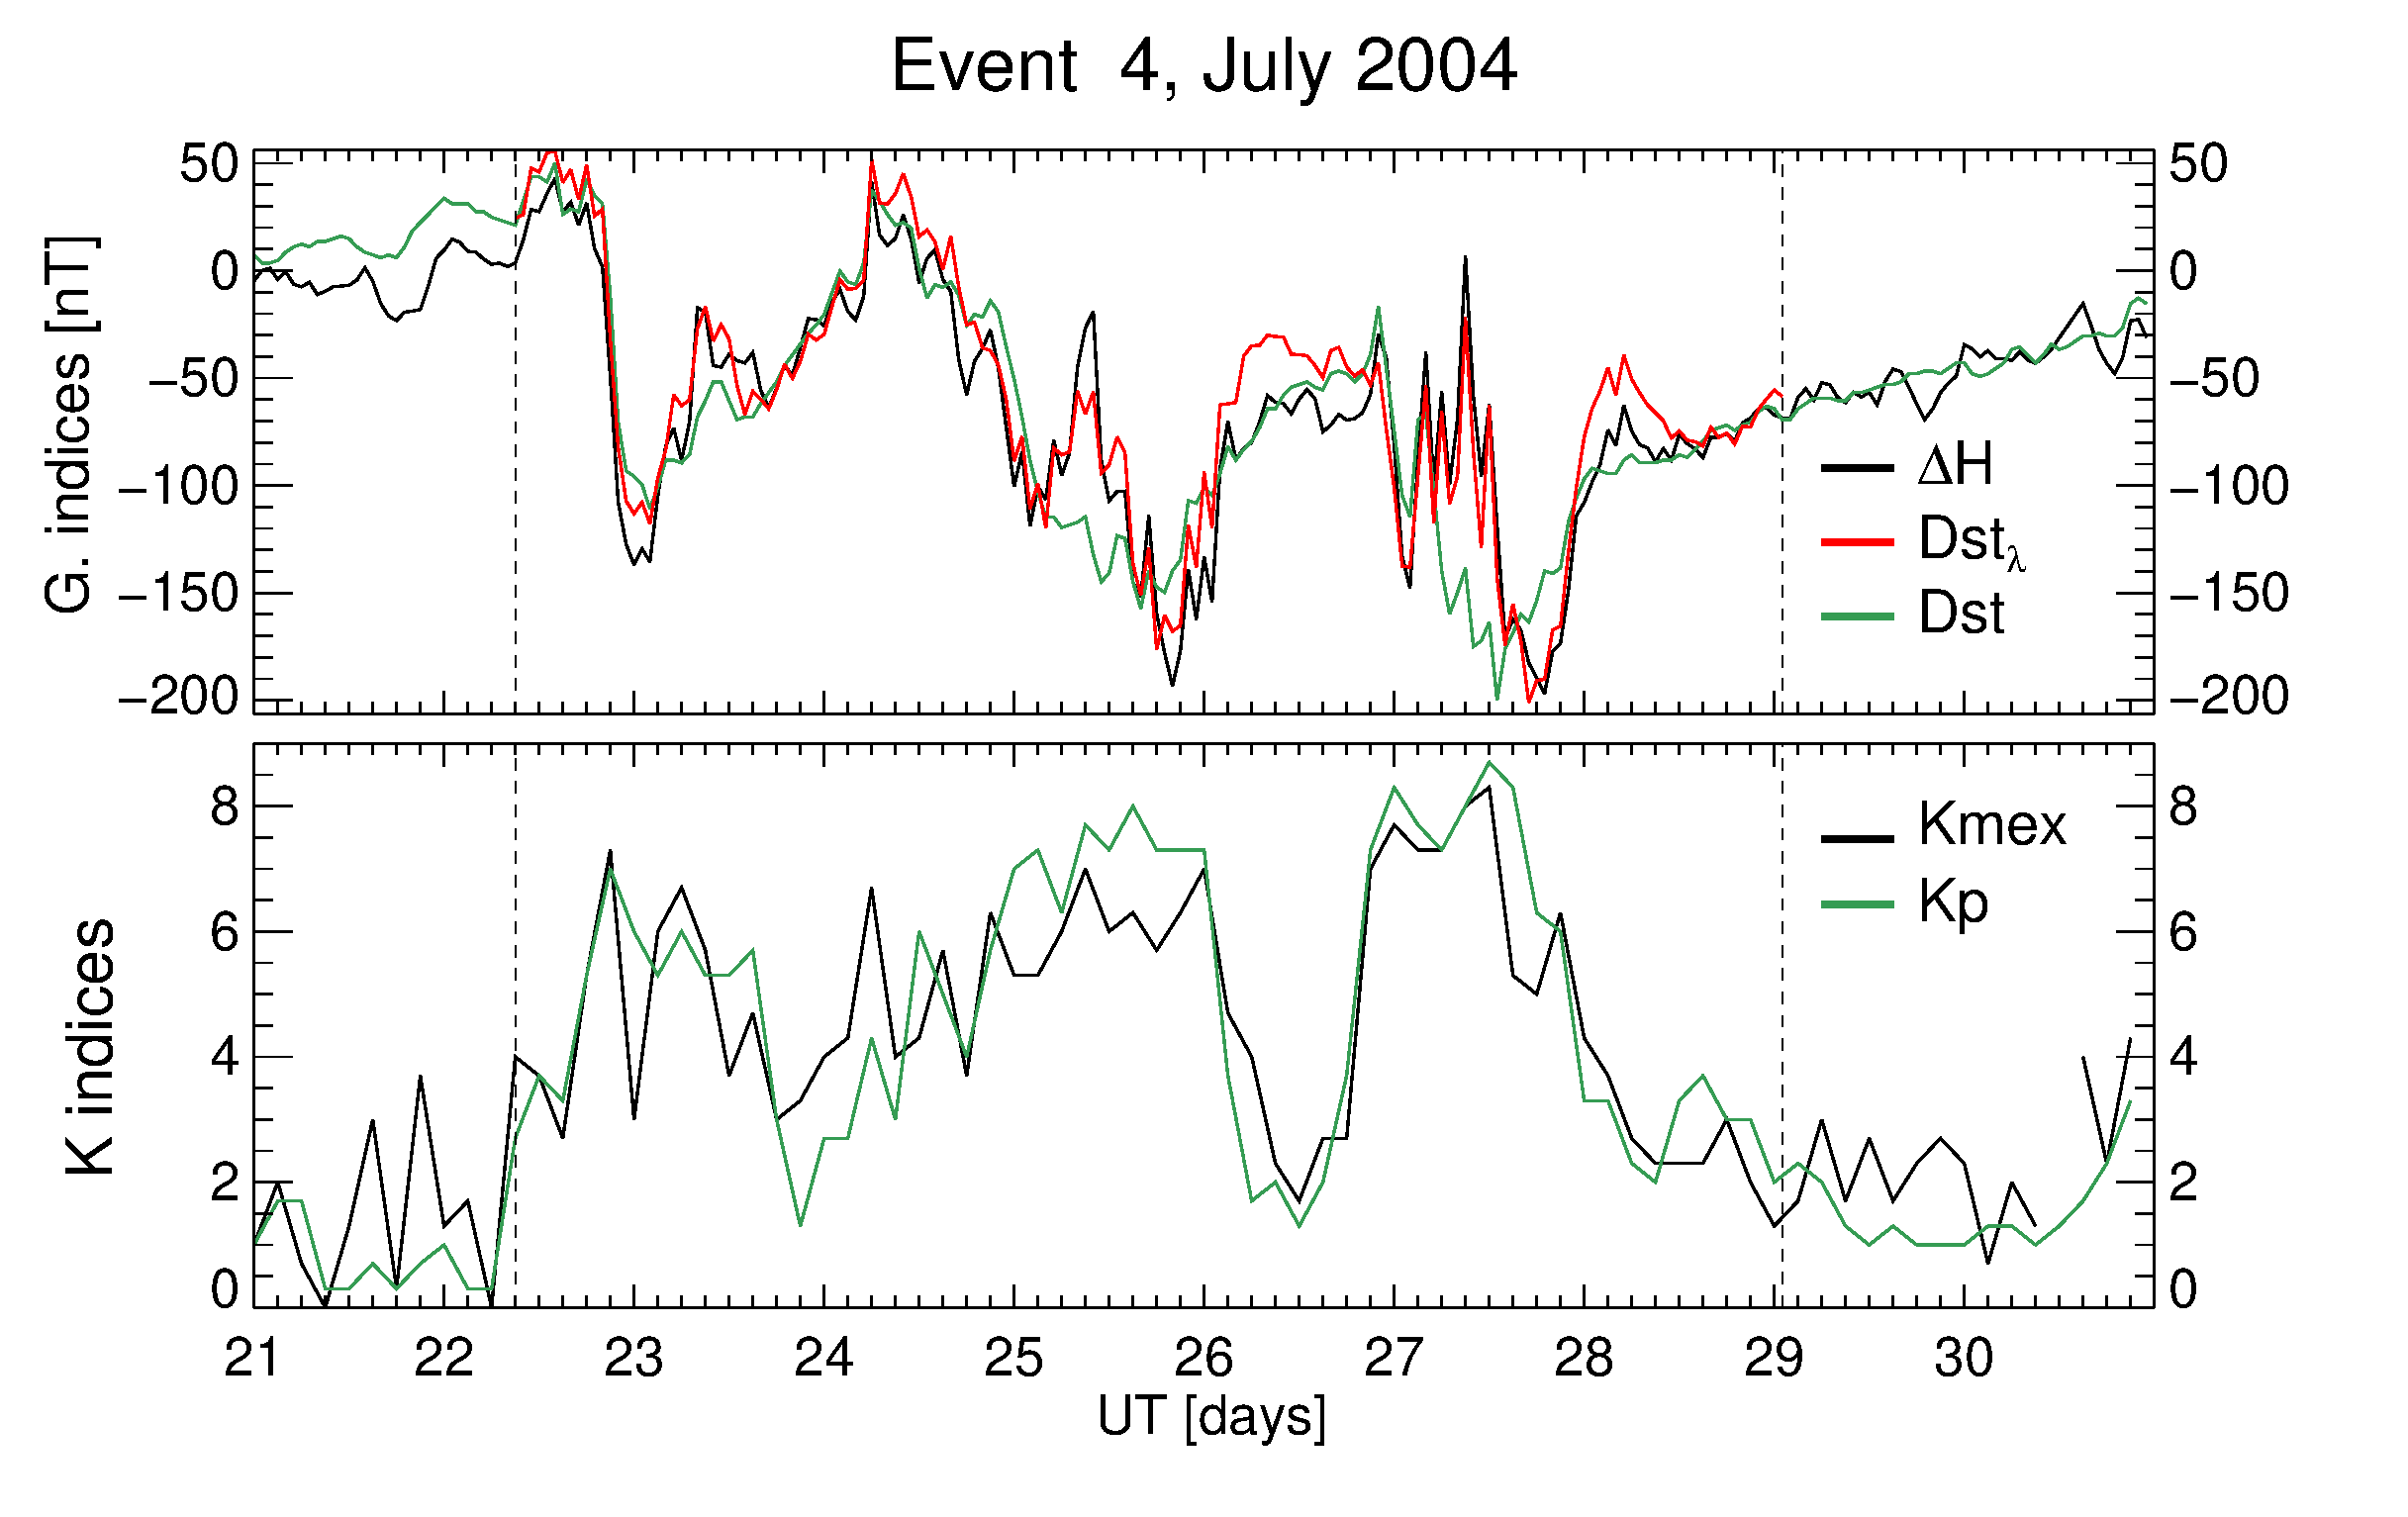
\includegraphics[width=6.0cm]{images/dH_approx/diono_valid_V4_2004-07-21.eps}      
       \centerline{\Large \bf   
      \hspace{0.275\textwidth}  \color{black}{}
       \hspace{0.295\textwidth}  \color{black}{}
         \hfill}
    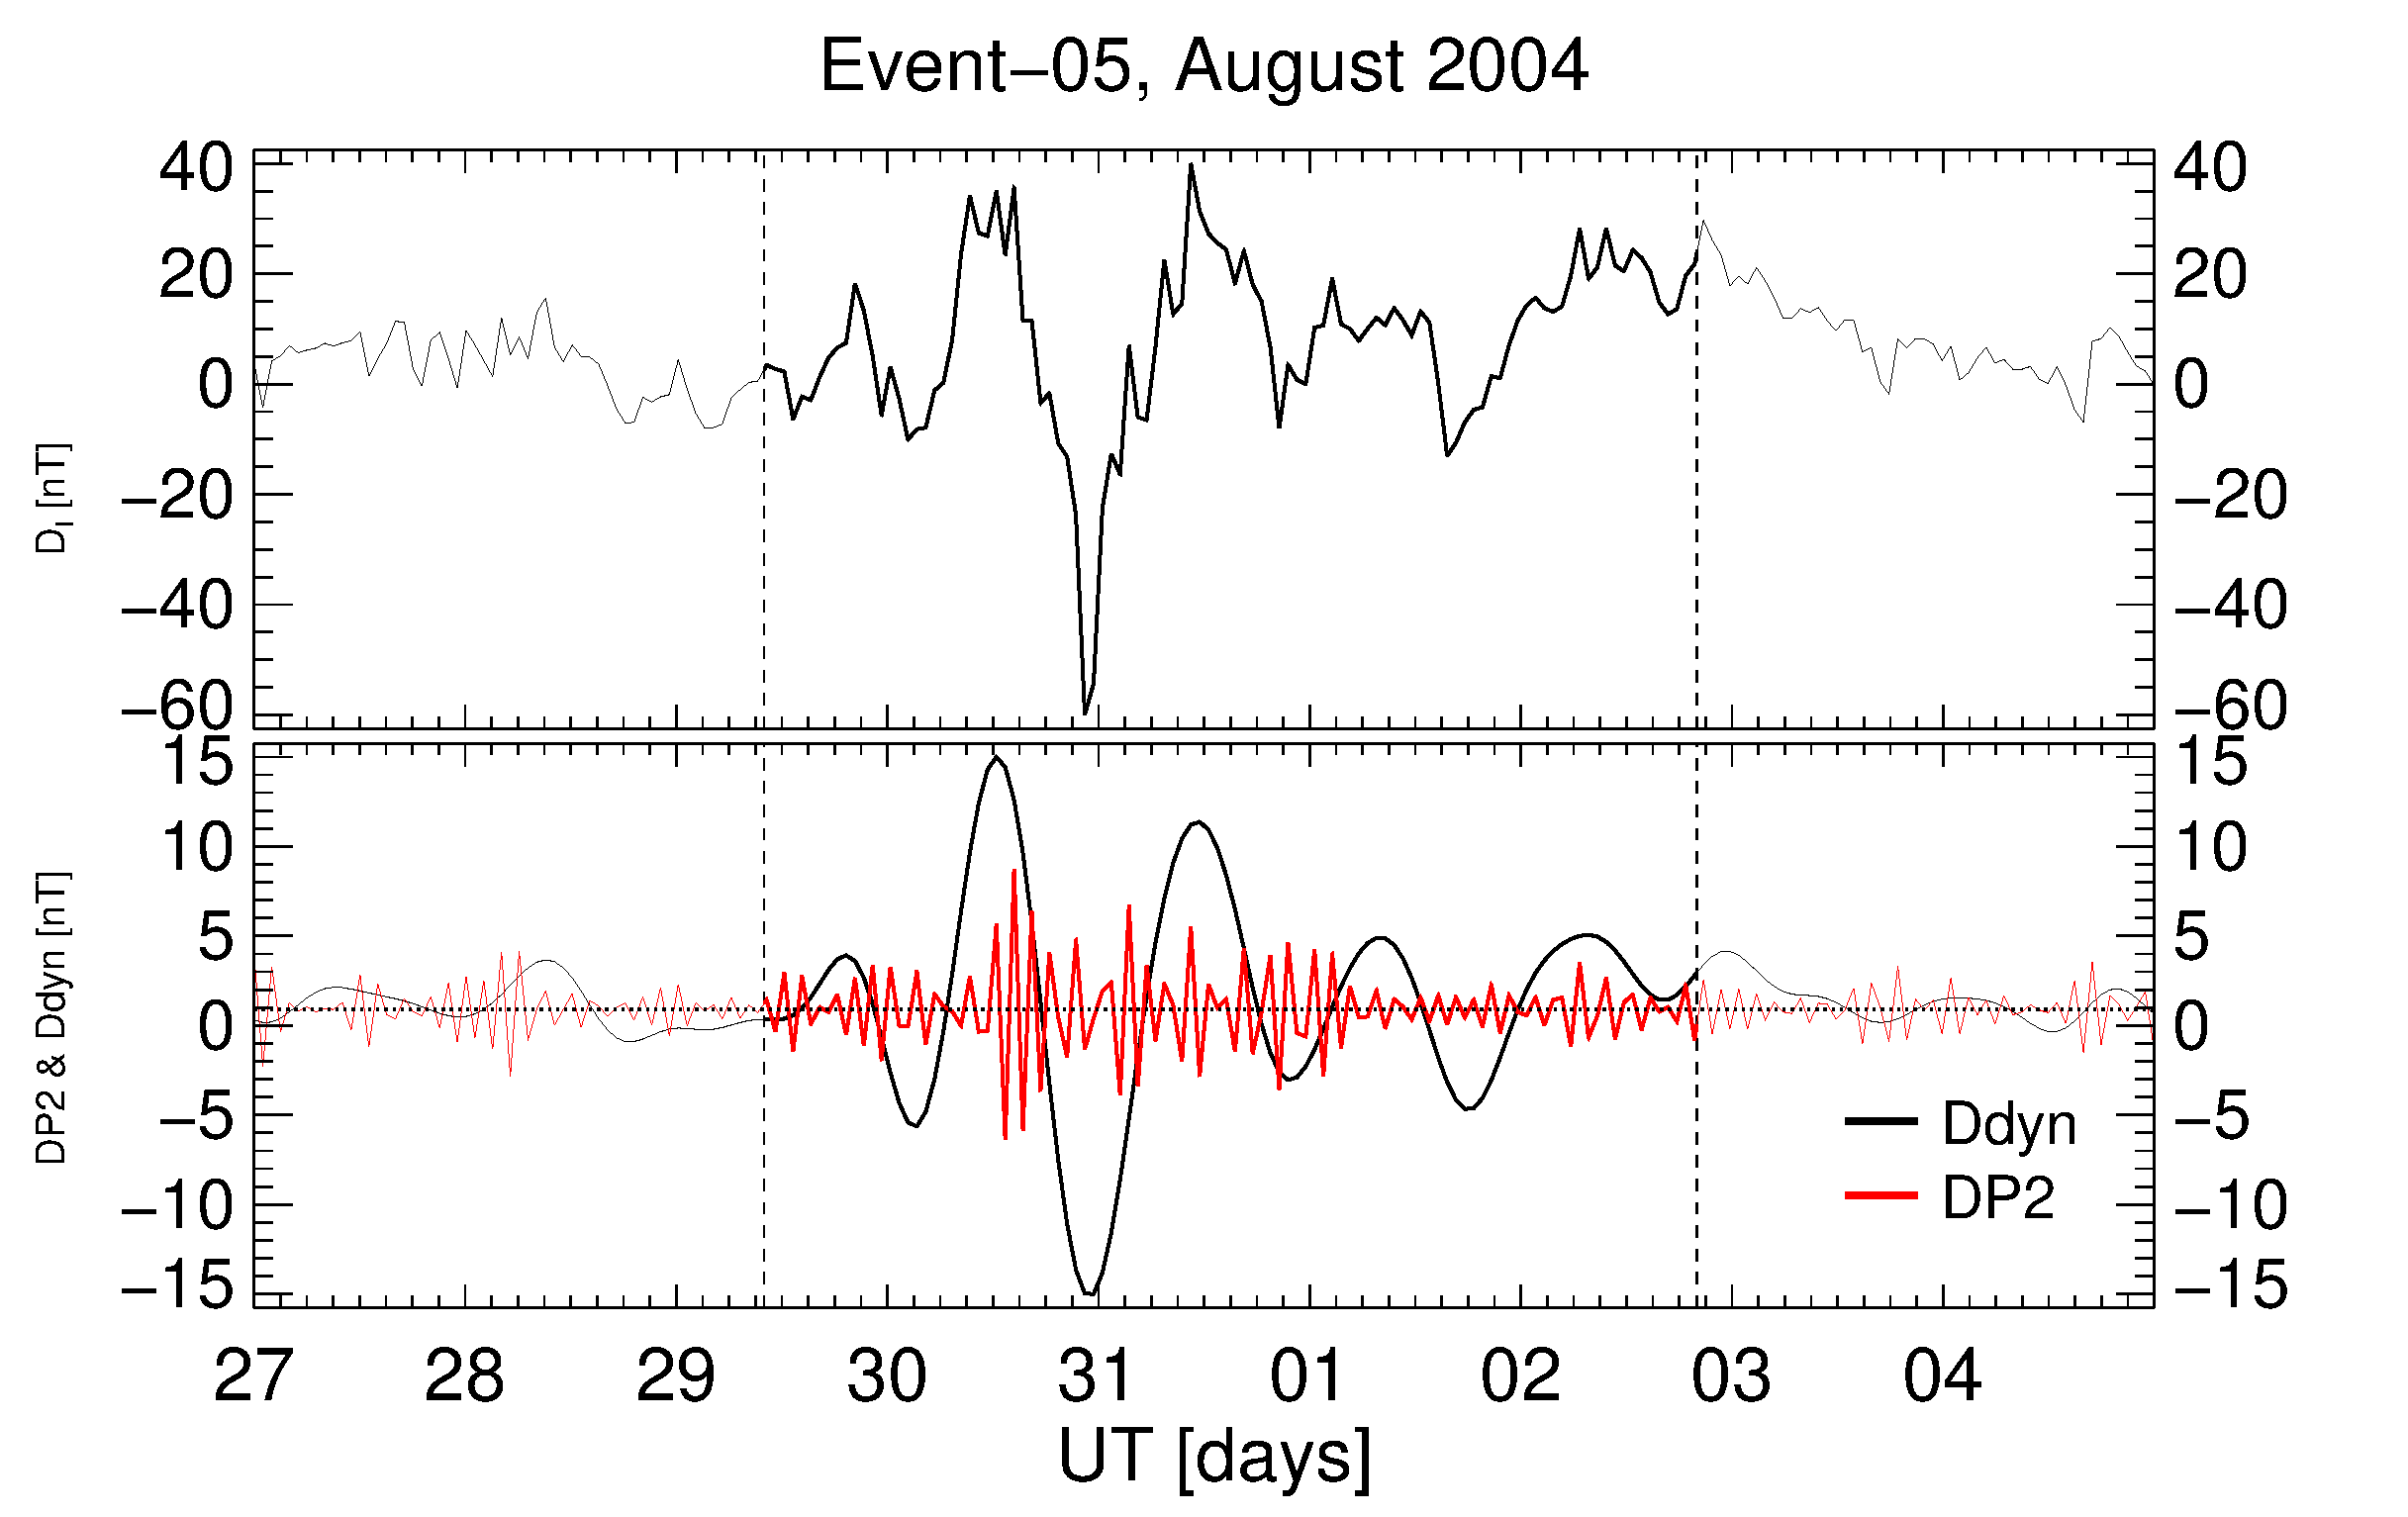
\includegraphics[width=6.0cm]{images/diono/iono_PI_V1_2004-08-27.eps}
    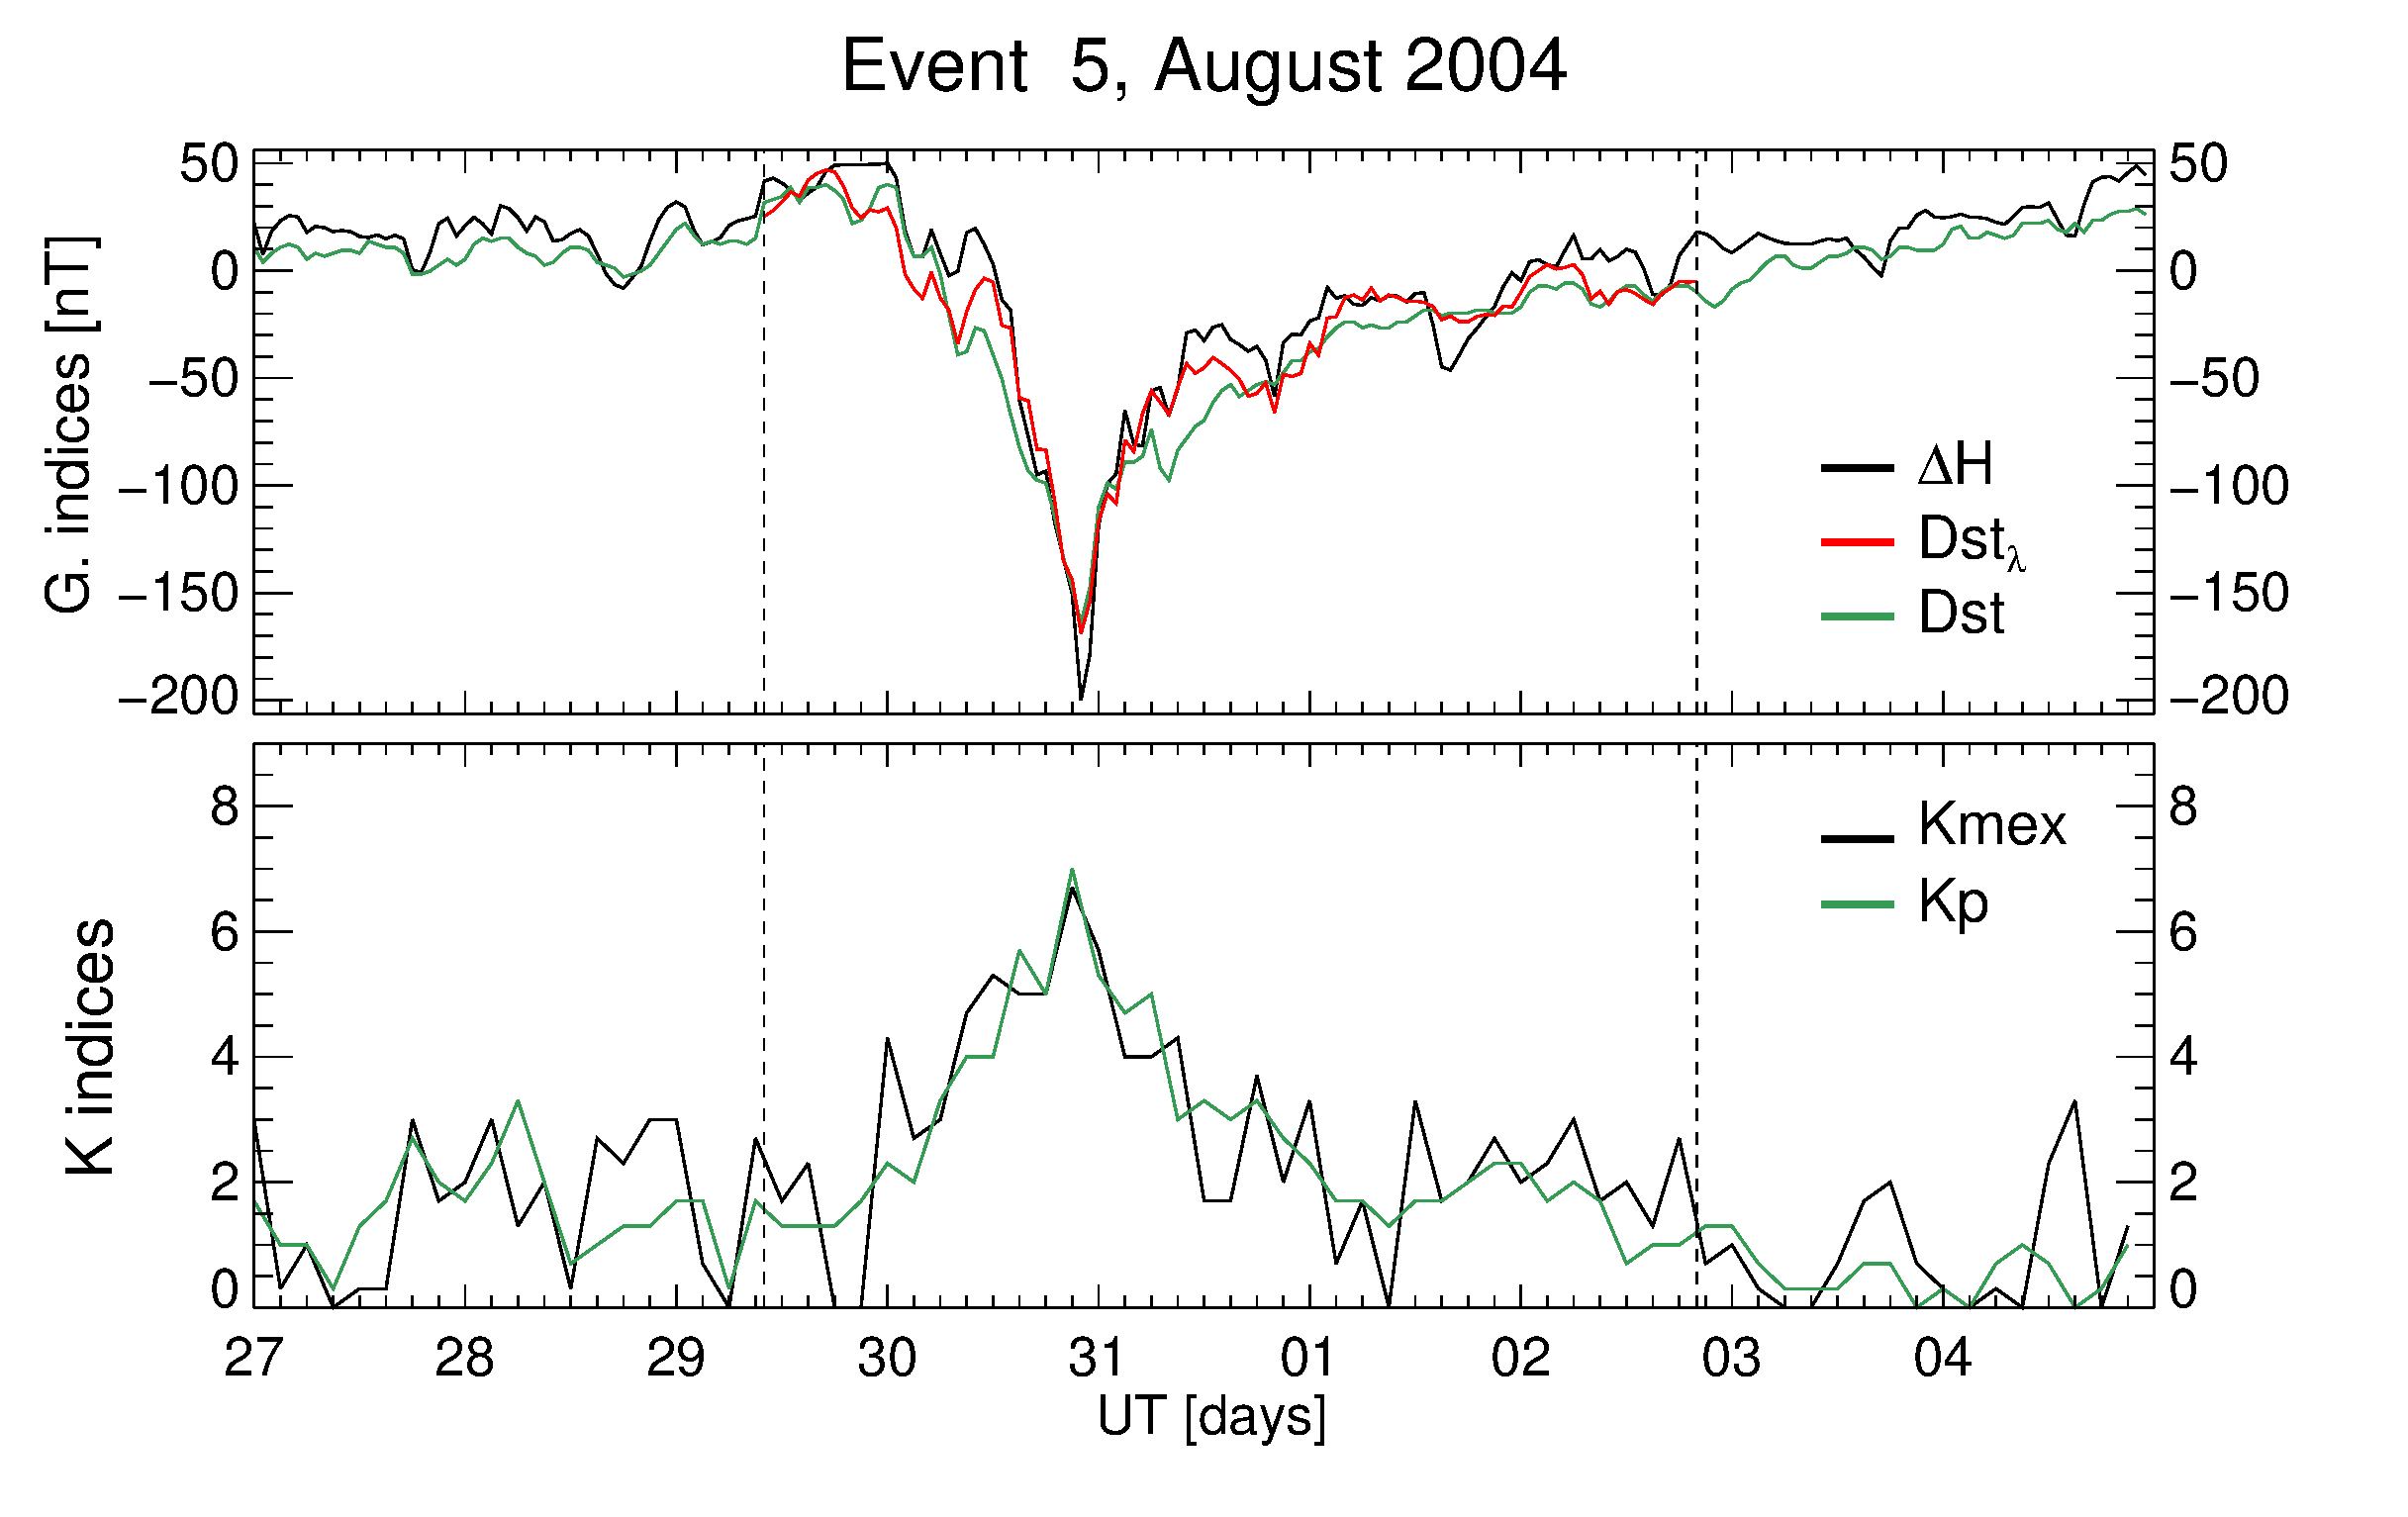
\includegraphics[width=6.0cm]{images/dH_approx/diono_valid_V4_2004-08-27.eps}            
       \caption{On the right side, top panels illustrate the contribution of Ionospheric Magnetic Disturbances, while bottom panels depict the isolated geomagnetic contributions of $Ddyn$ and $DP2$. The vertical dashed lines highlight the geomagnetic storm time period during which such calculations are valid. On the left side, green lines represent planetary indices, while black lines denote local indices. Additionally, red lines represent the approximation of $\Delta H$ at top, while bottom showcases the comparison of local $K$ (black line) and planetary $K$ (green line).
       }
    \label{fig:iono_resp2}
\end{figure*}


\begin{figure*}[h!]
    \centering
    \centerline{\Large \bf   
      %\hspace{0.18\textwidth}  \color{black}{\Large{Res}}
       %\hspace{0.28\textwidth}  \color{black}{\Large{Res+TC}}
         \hfill}
          \centerline{\Large \bf   
      \hspace{0.26\textwidth}  \color{black}{}
       \hspace{0.31\textwidth}  \color{black}{}
         \hfill}
    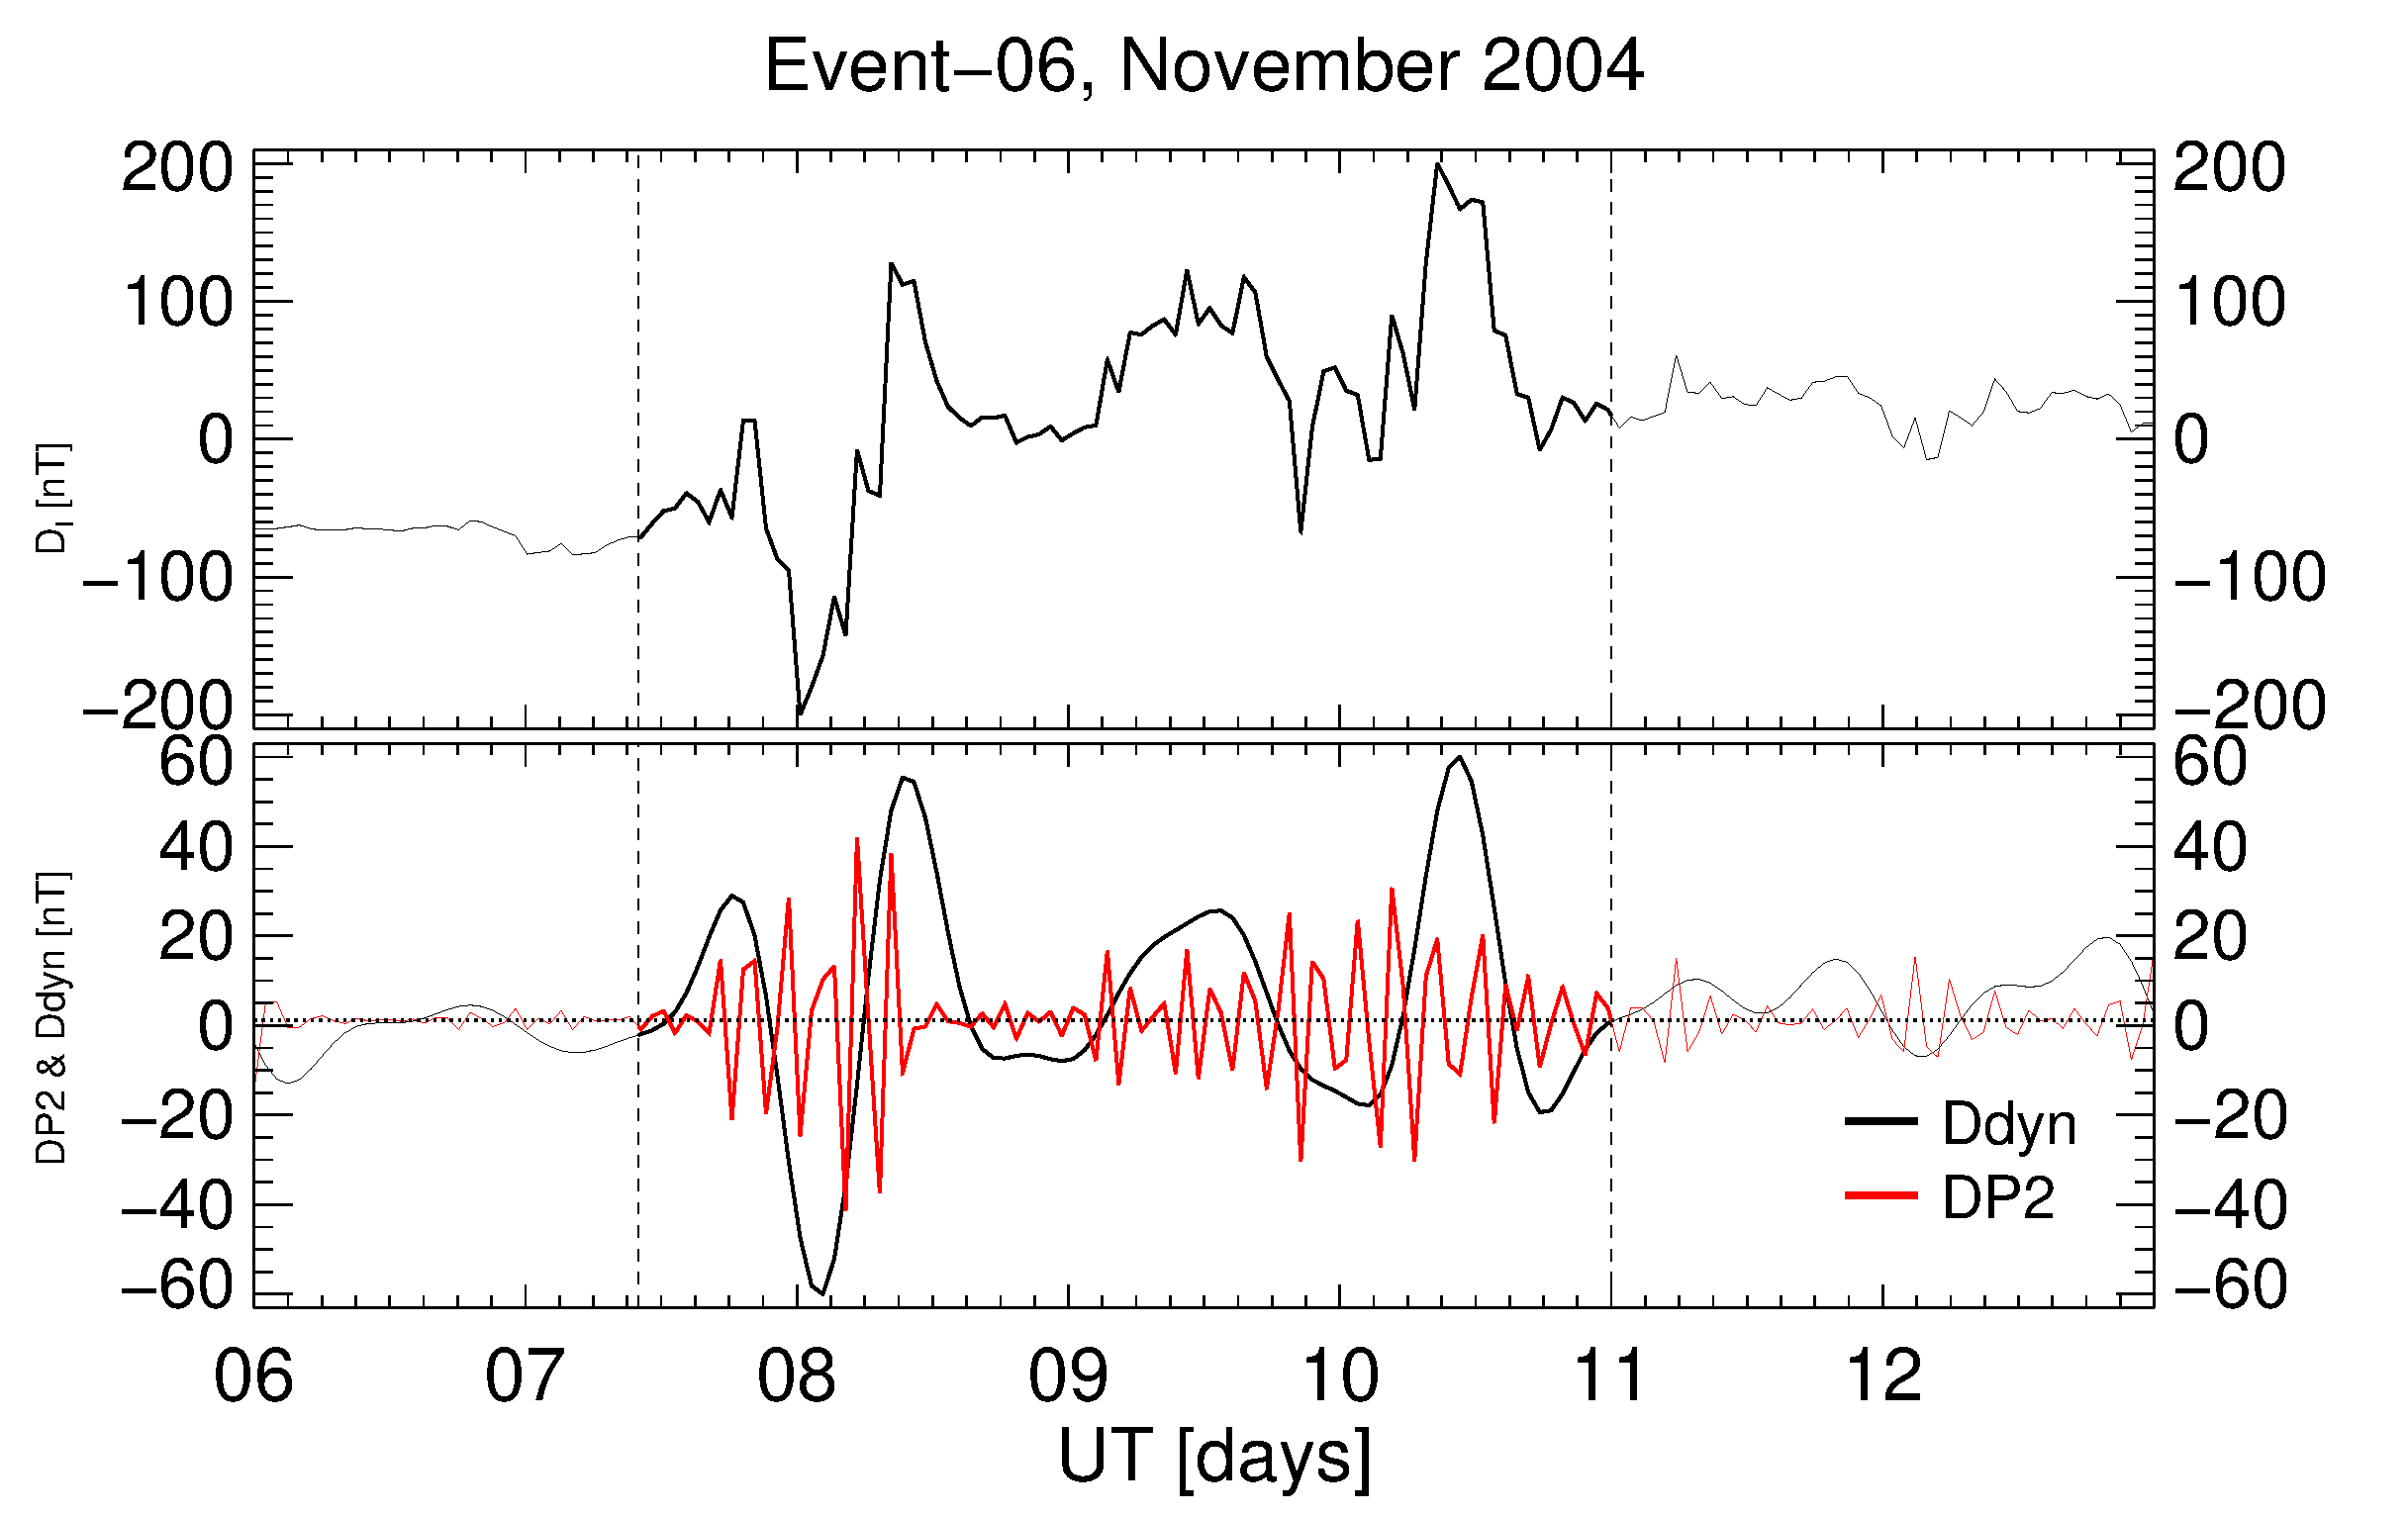
\includegraphics[width=6.0cm]{images/diono/iono_PI_V1_2004-11-06.eps}
	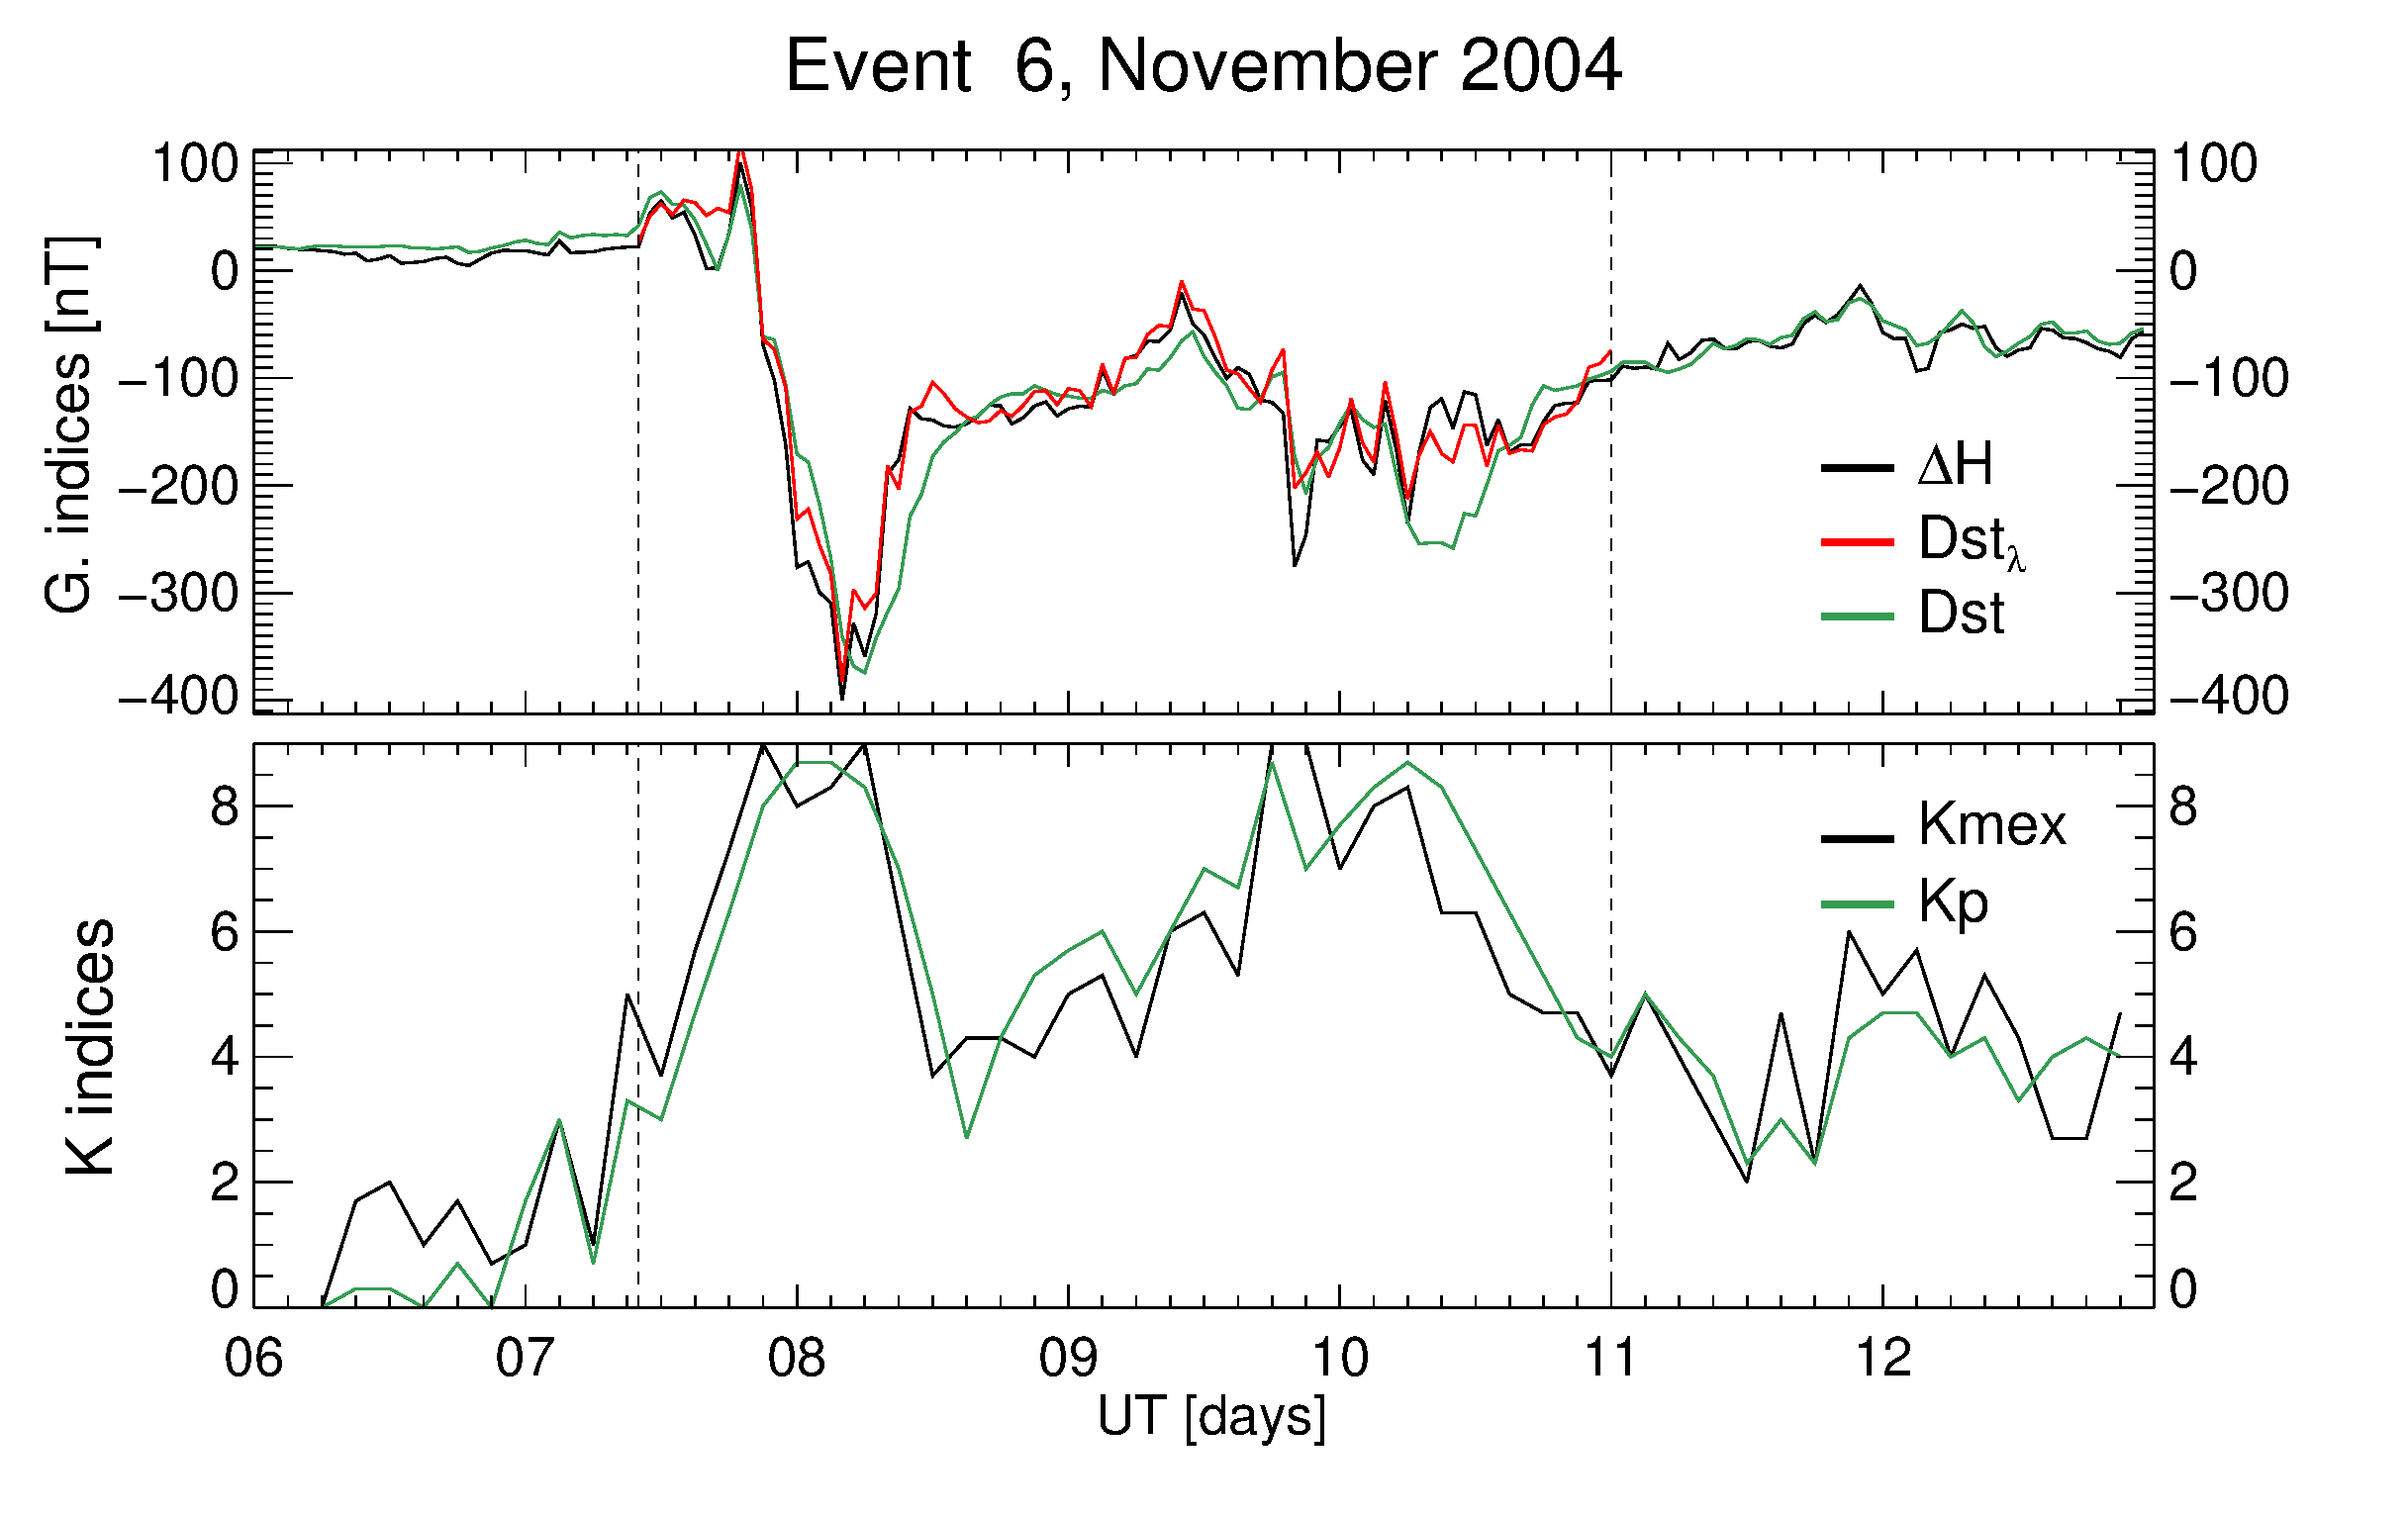
\includegraphics[width=6.0cm]{images/dH_approx/diono_valid_V4_2004-11-06.eps}    
     \centerline{\Large \bf   
      \hspace{0.275\textwidth}  \color{black}{}
       \hspace{0.295\textwidth}  \color{black}{}
         \hfill}
    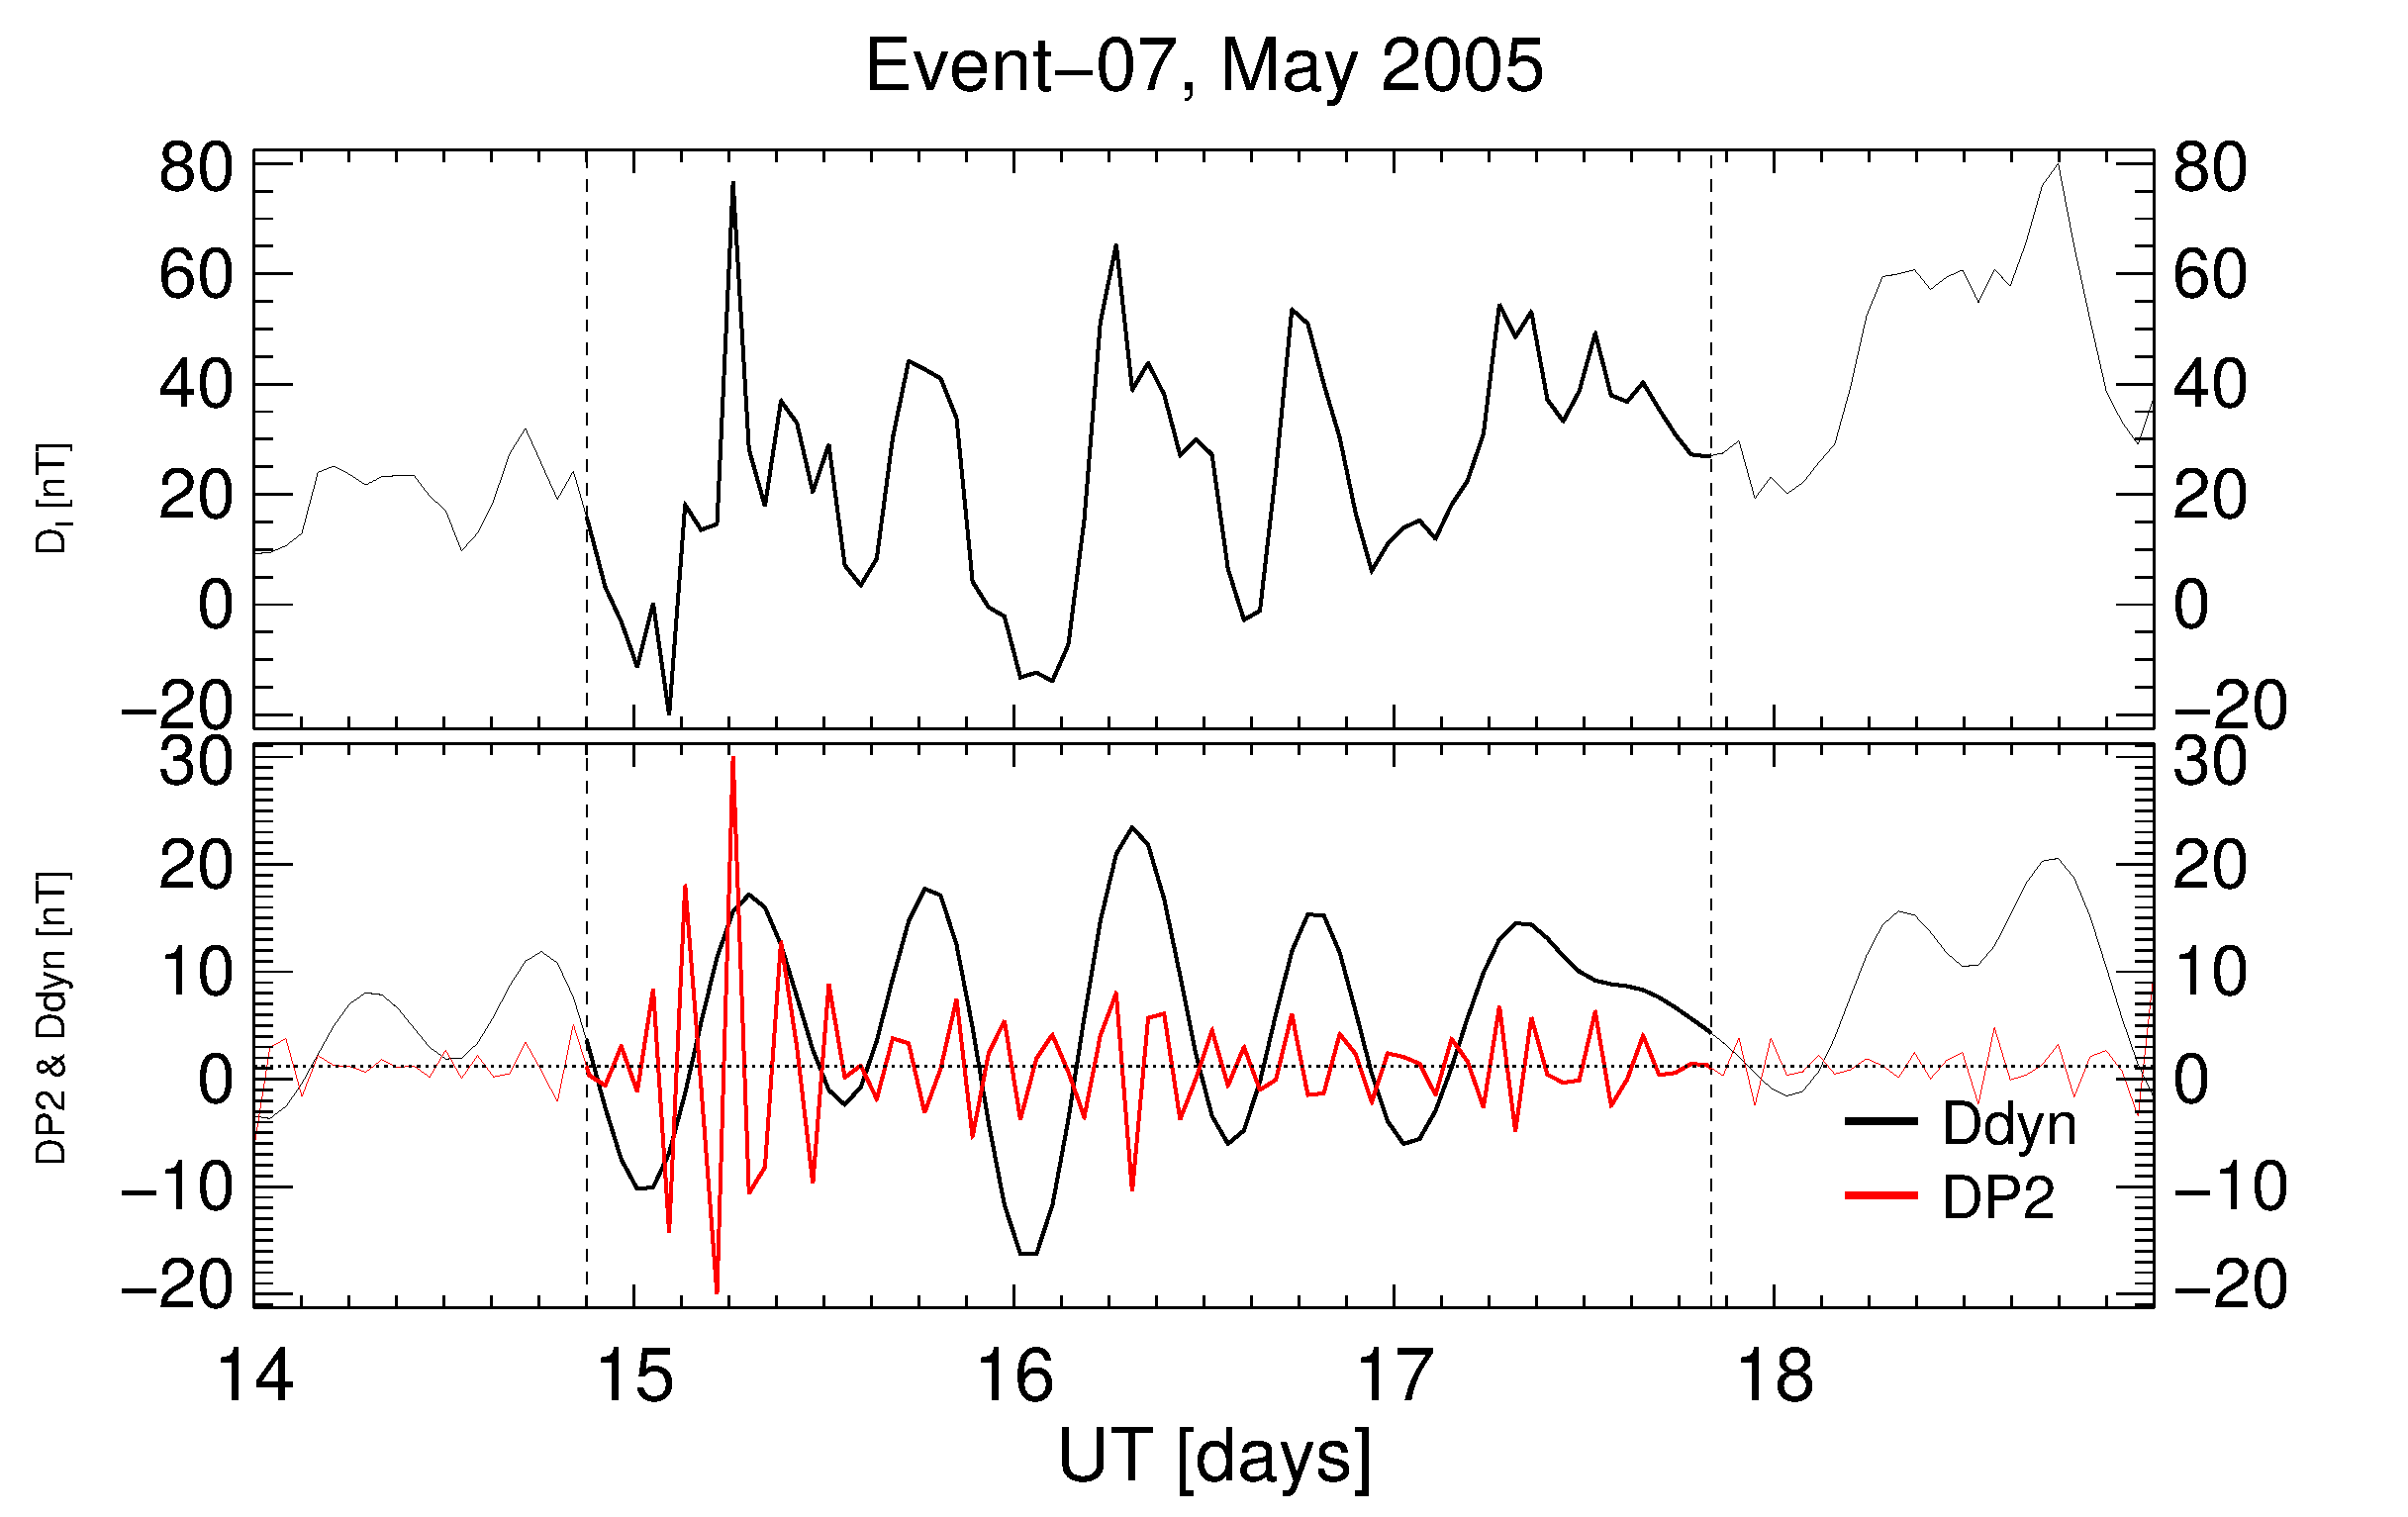
\includegraphics[width=6.0cm]{images/diono/iono_PI_V1_2005-05-14.eps}   
	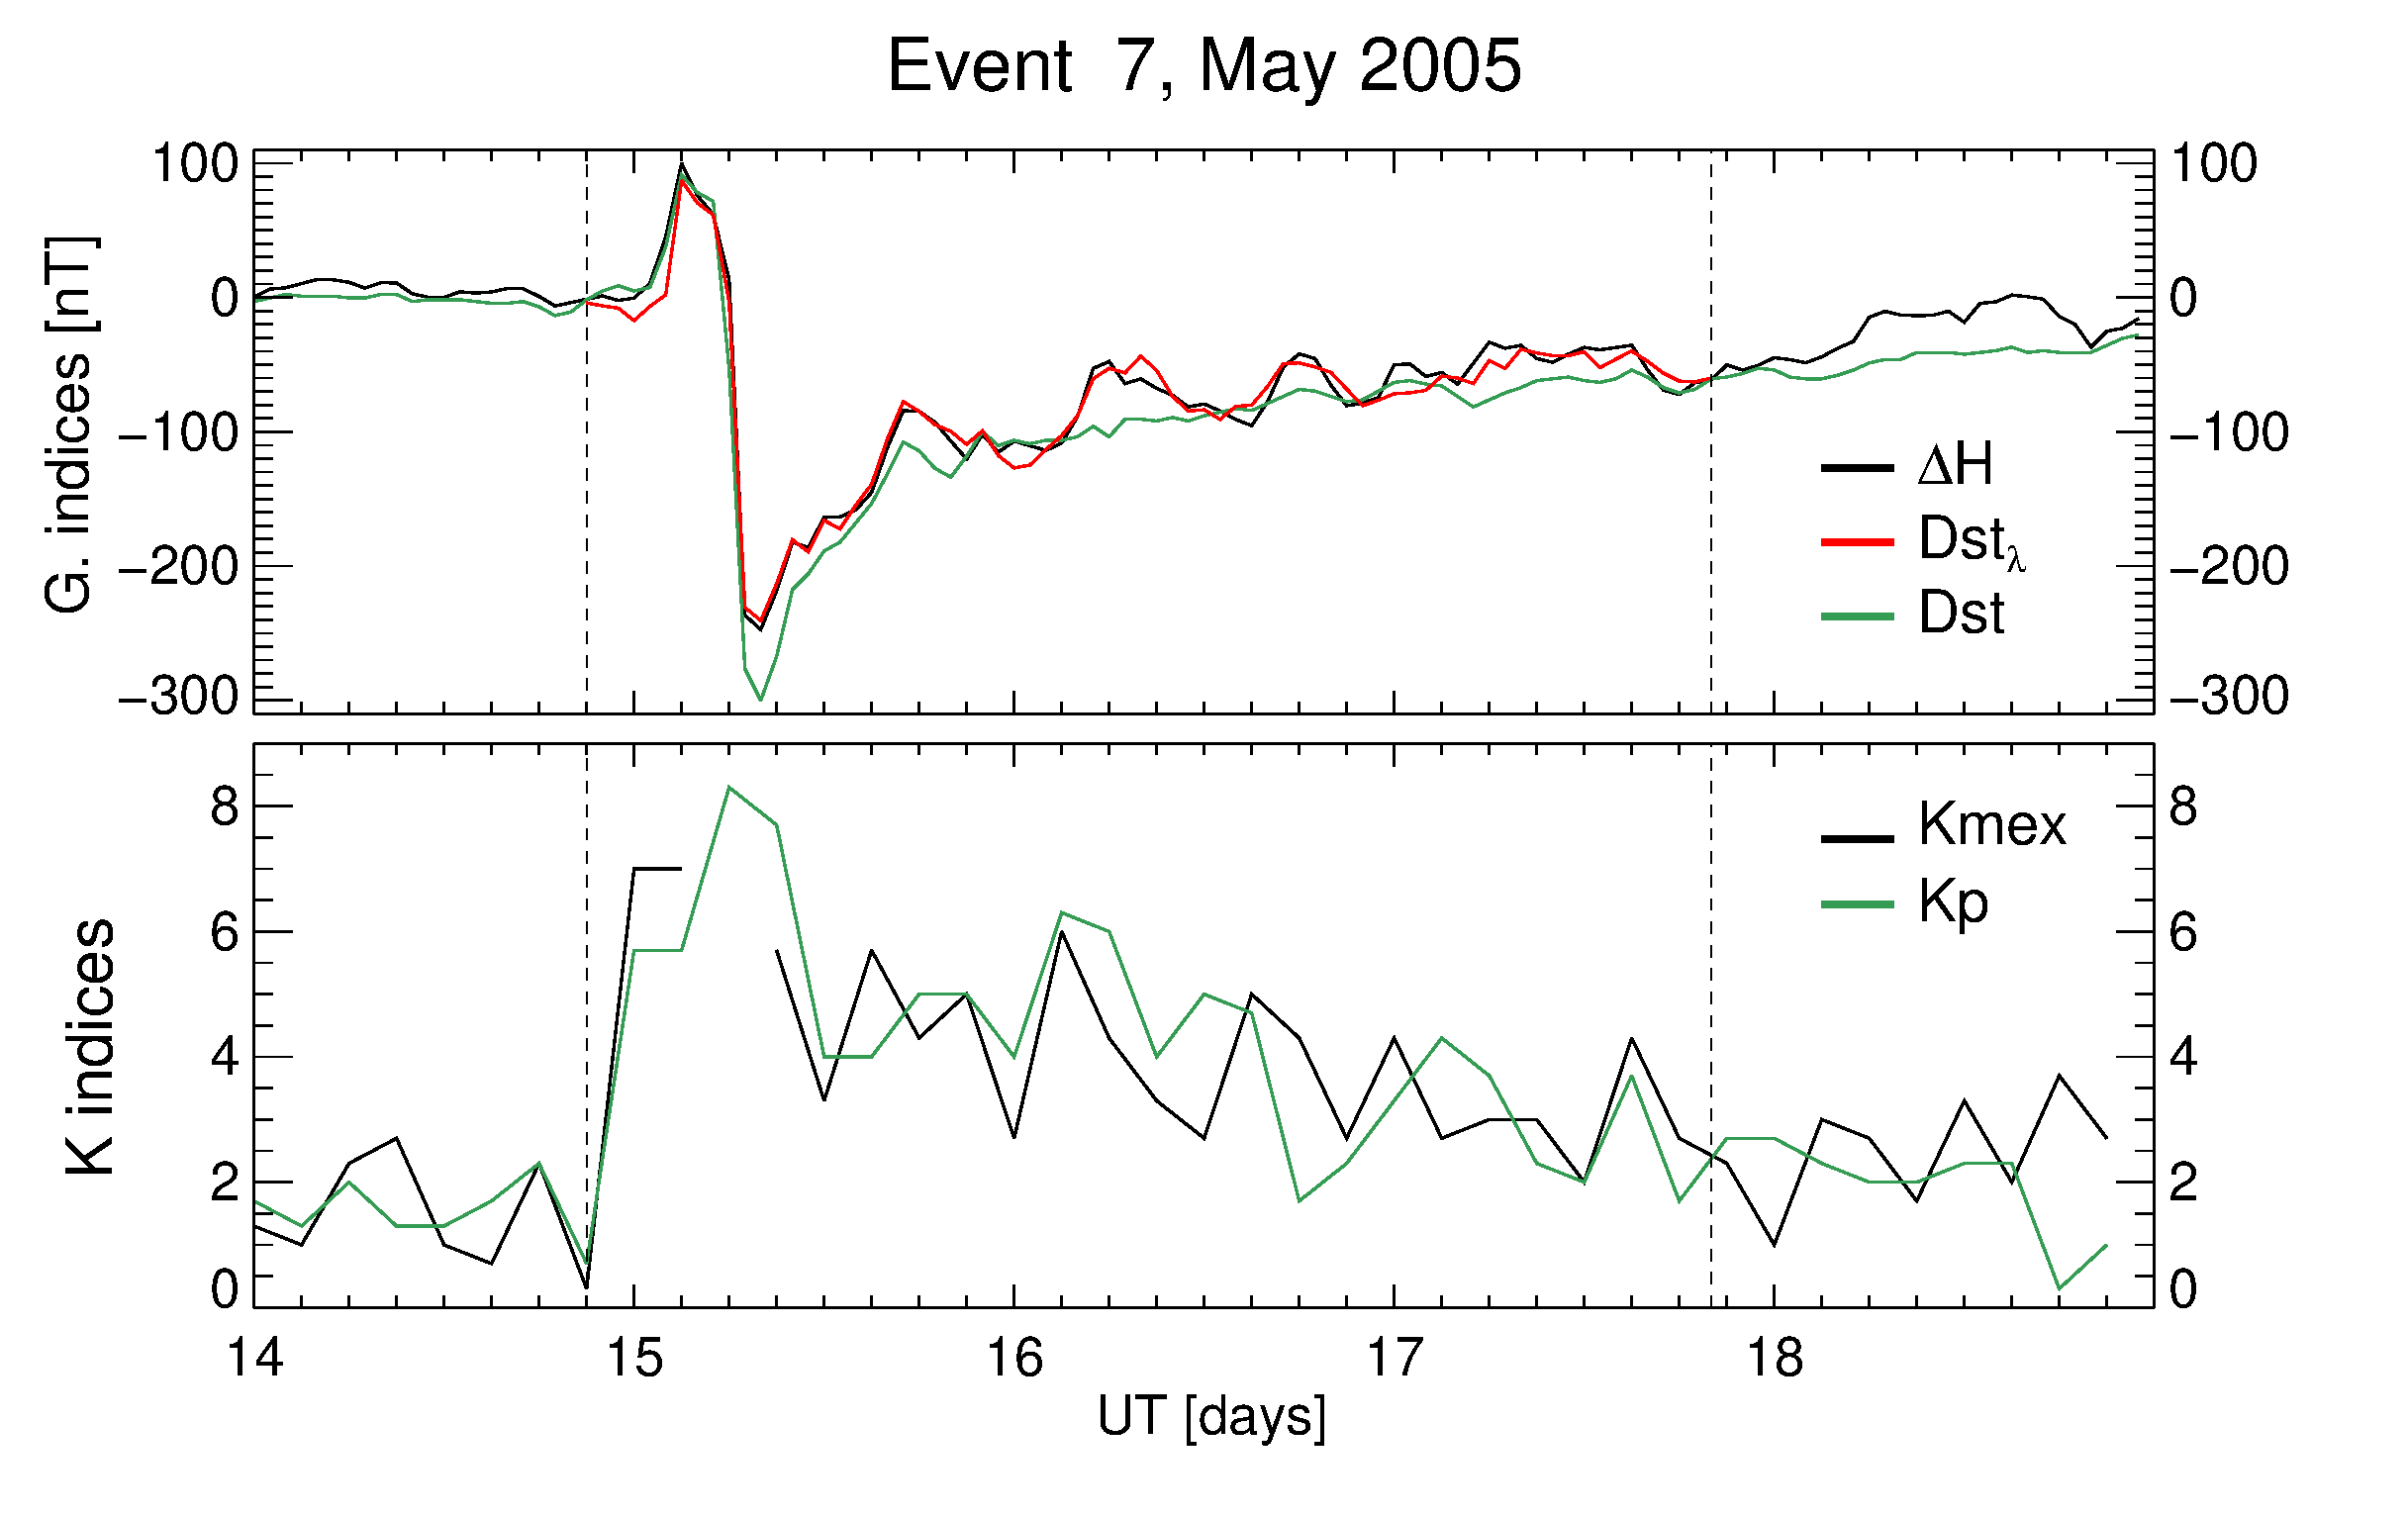
\includegraphics[width=6.0cm]{images/dH_approx/diono_valid_V4_2005-05-14.eps}        
     \centerline{\Large \bf   
      \hspace{0.275\textwidth}  \color{black}{}
       \hspace{0.295\textwidth}  \color{black}{}
         \hfill}
	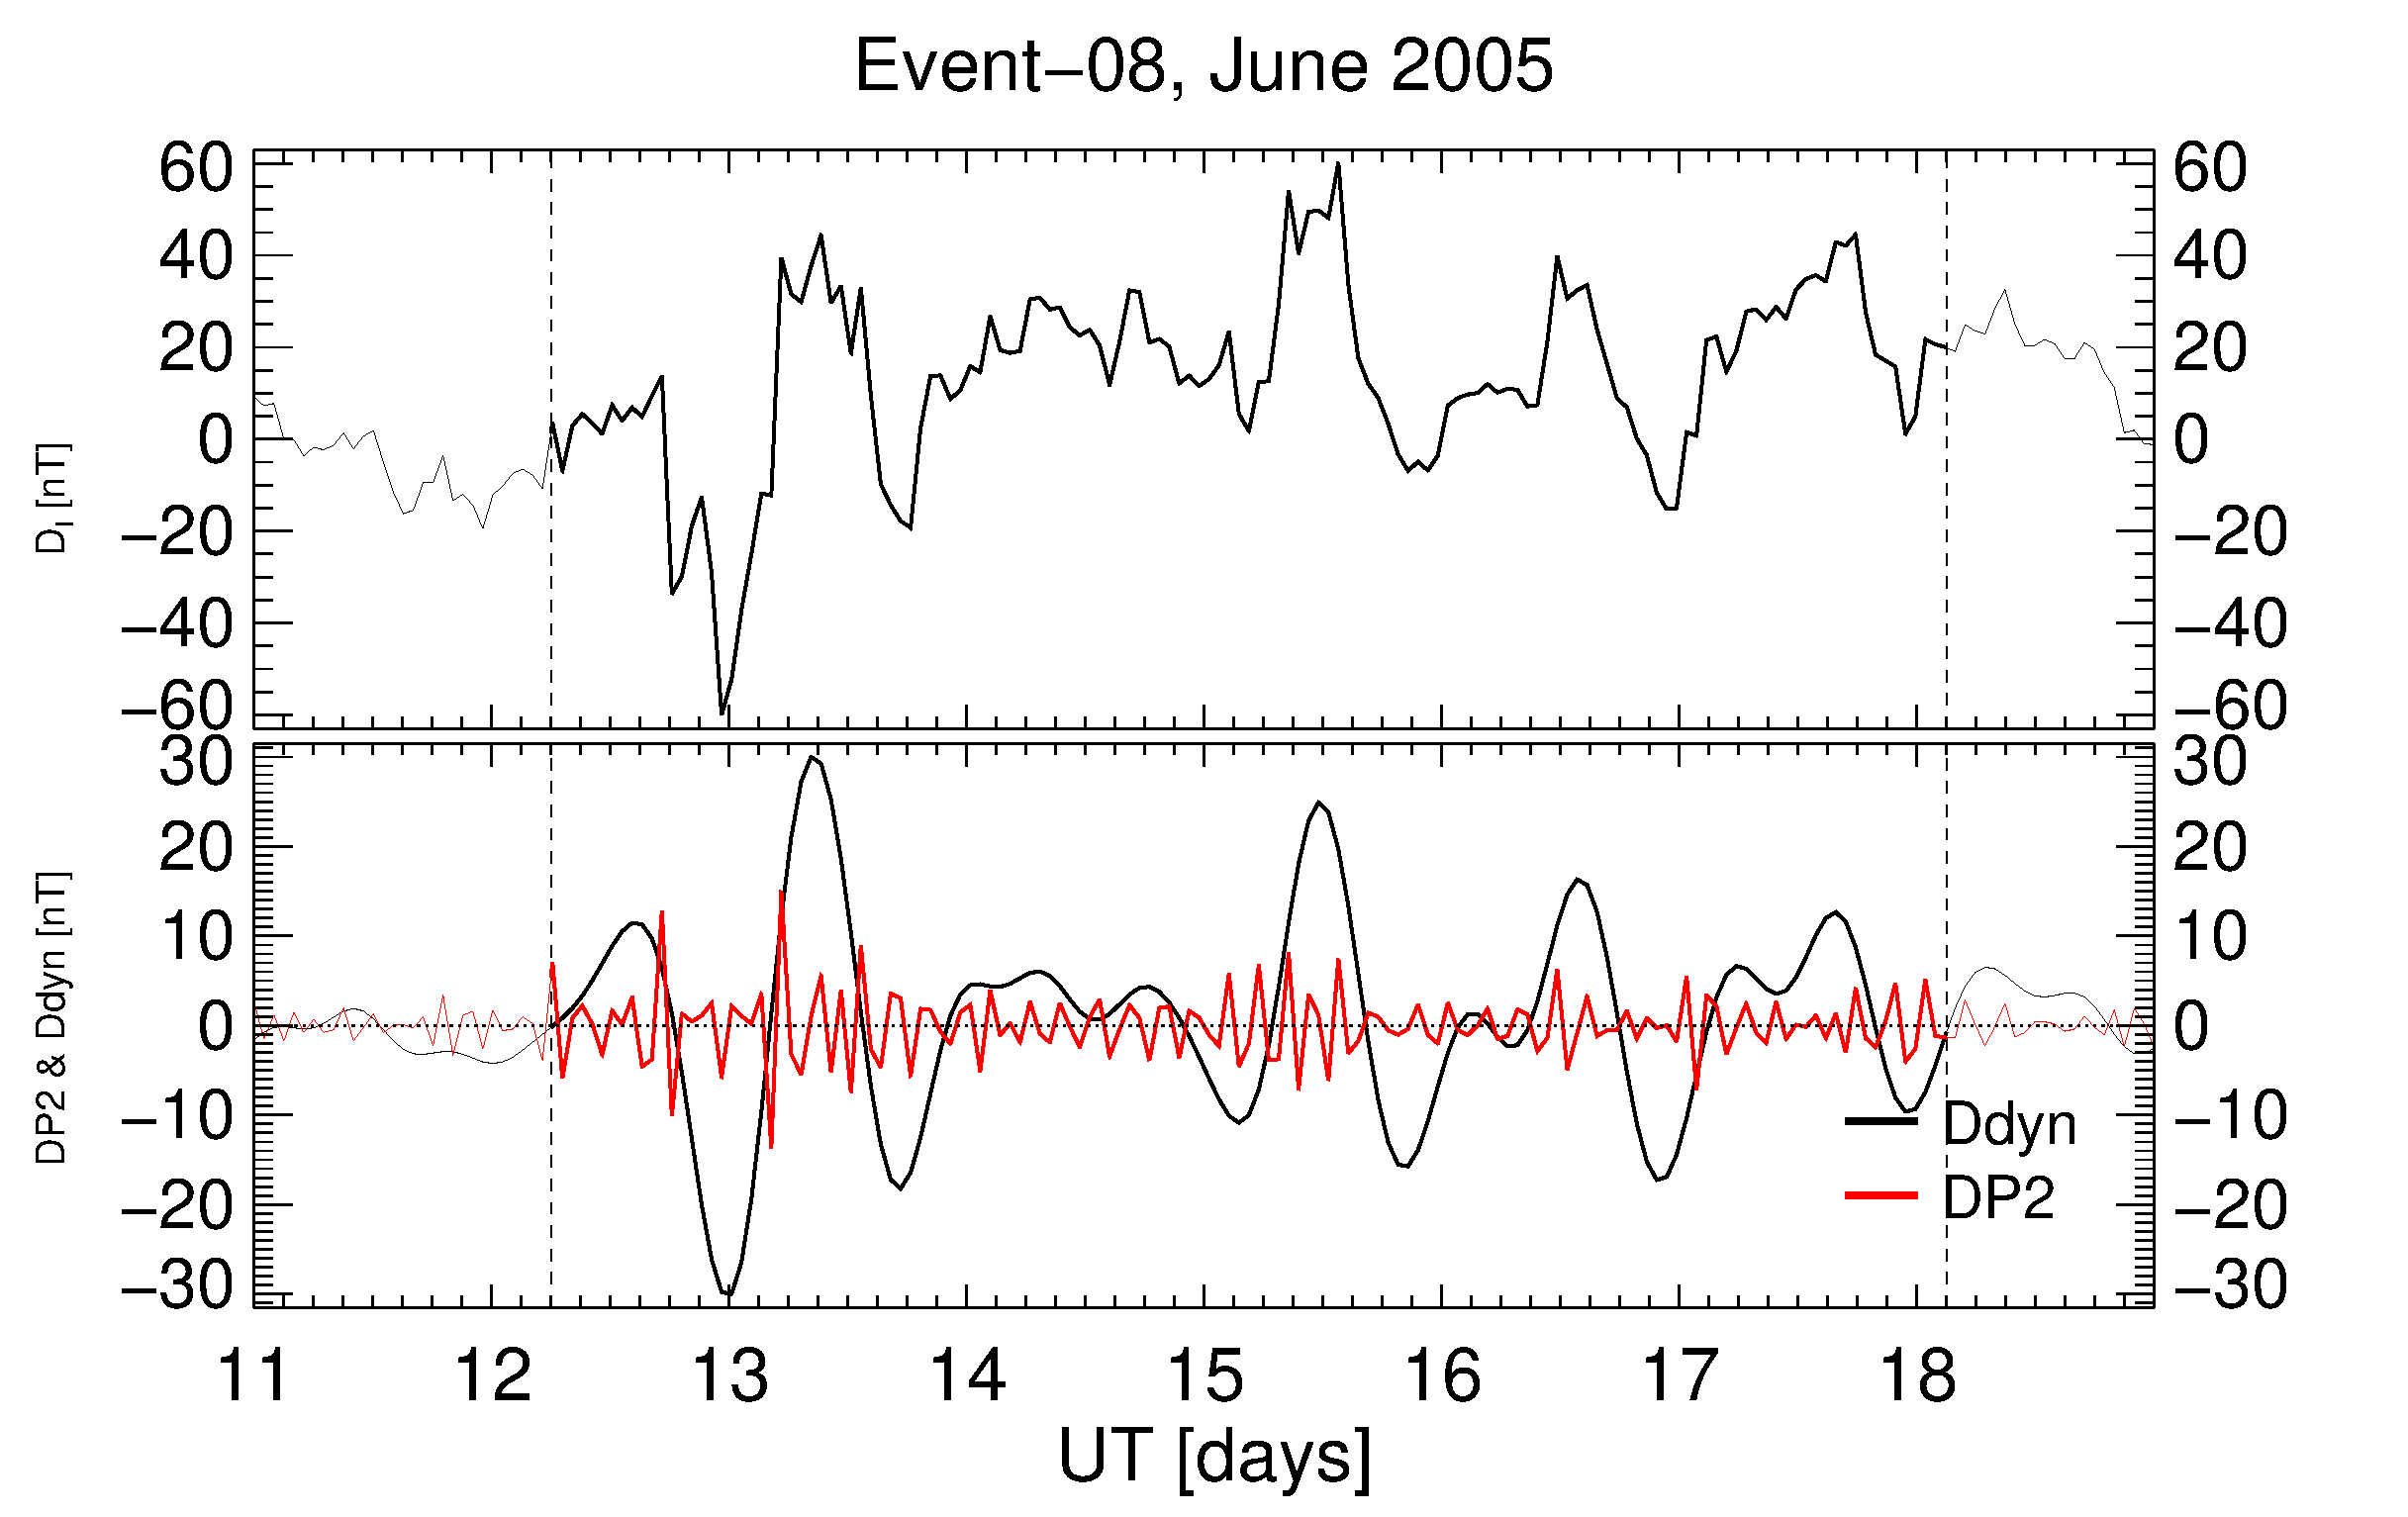
\includegraphics[width=6.0cm]{images/diono/iono_PI_V1_2005-06-11.eps}     
	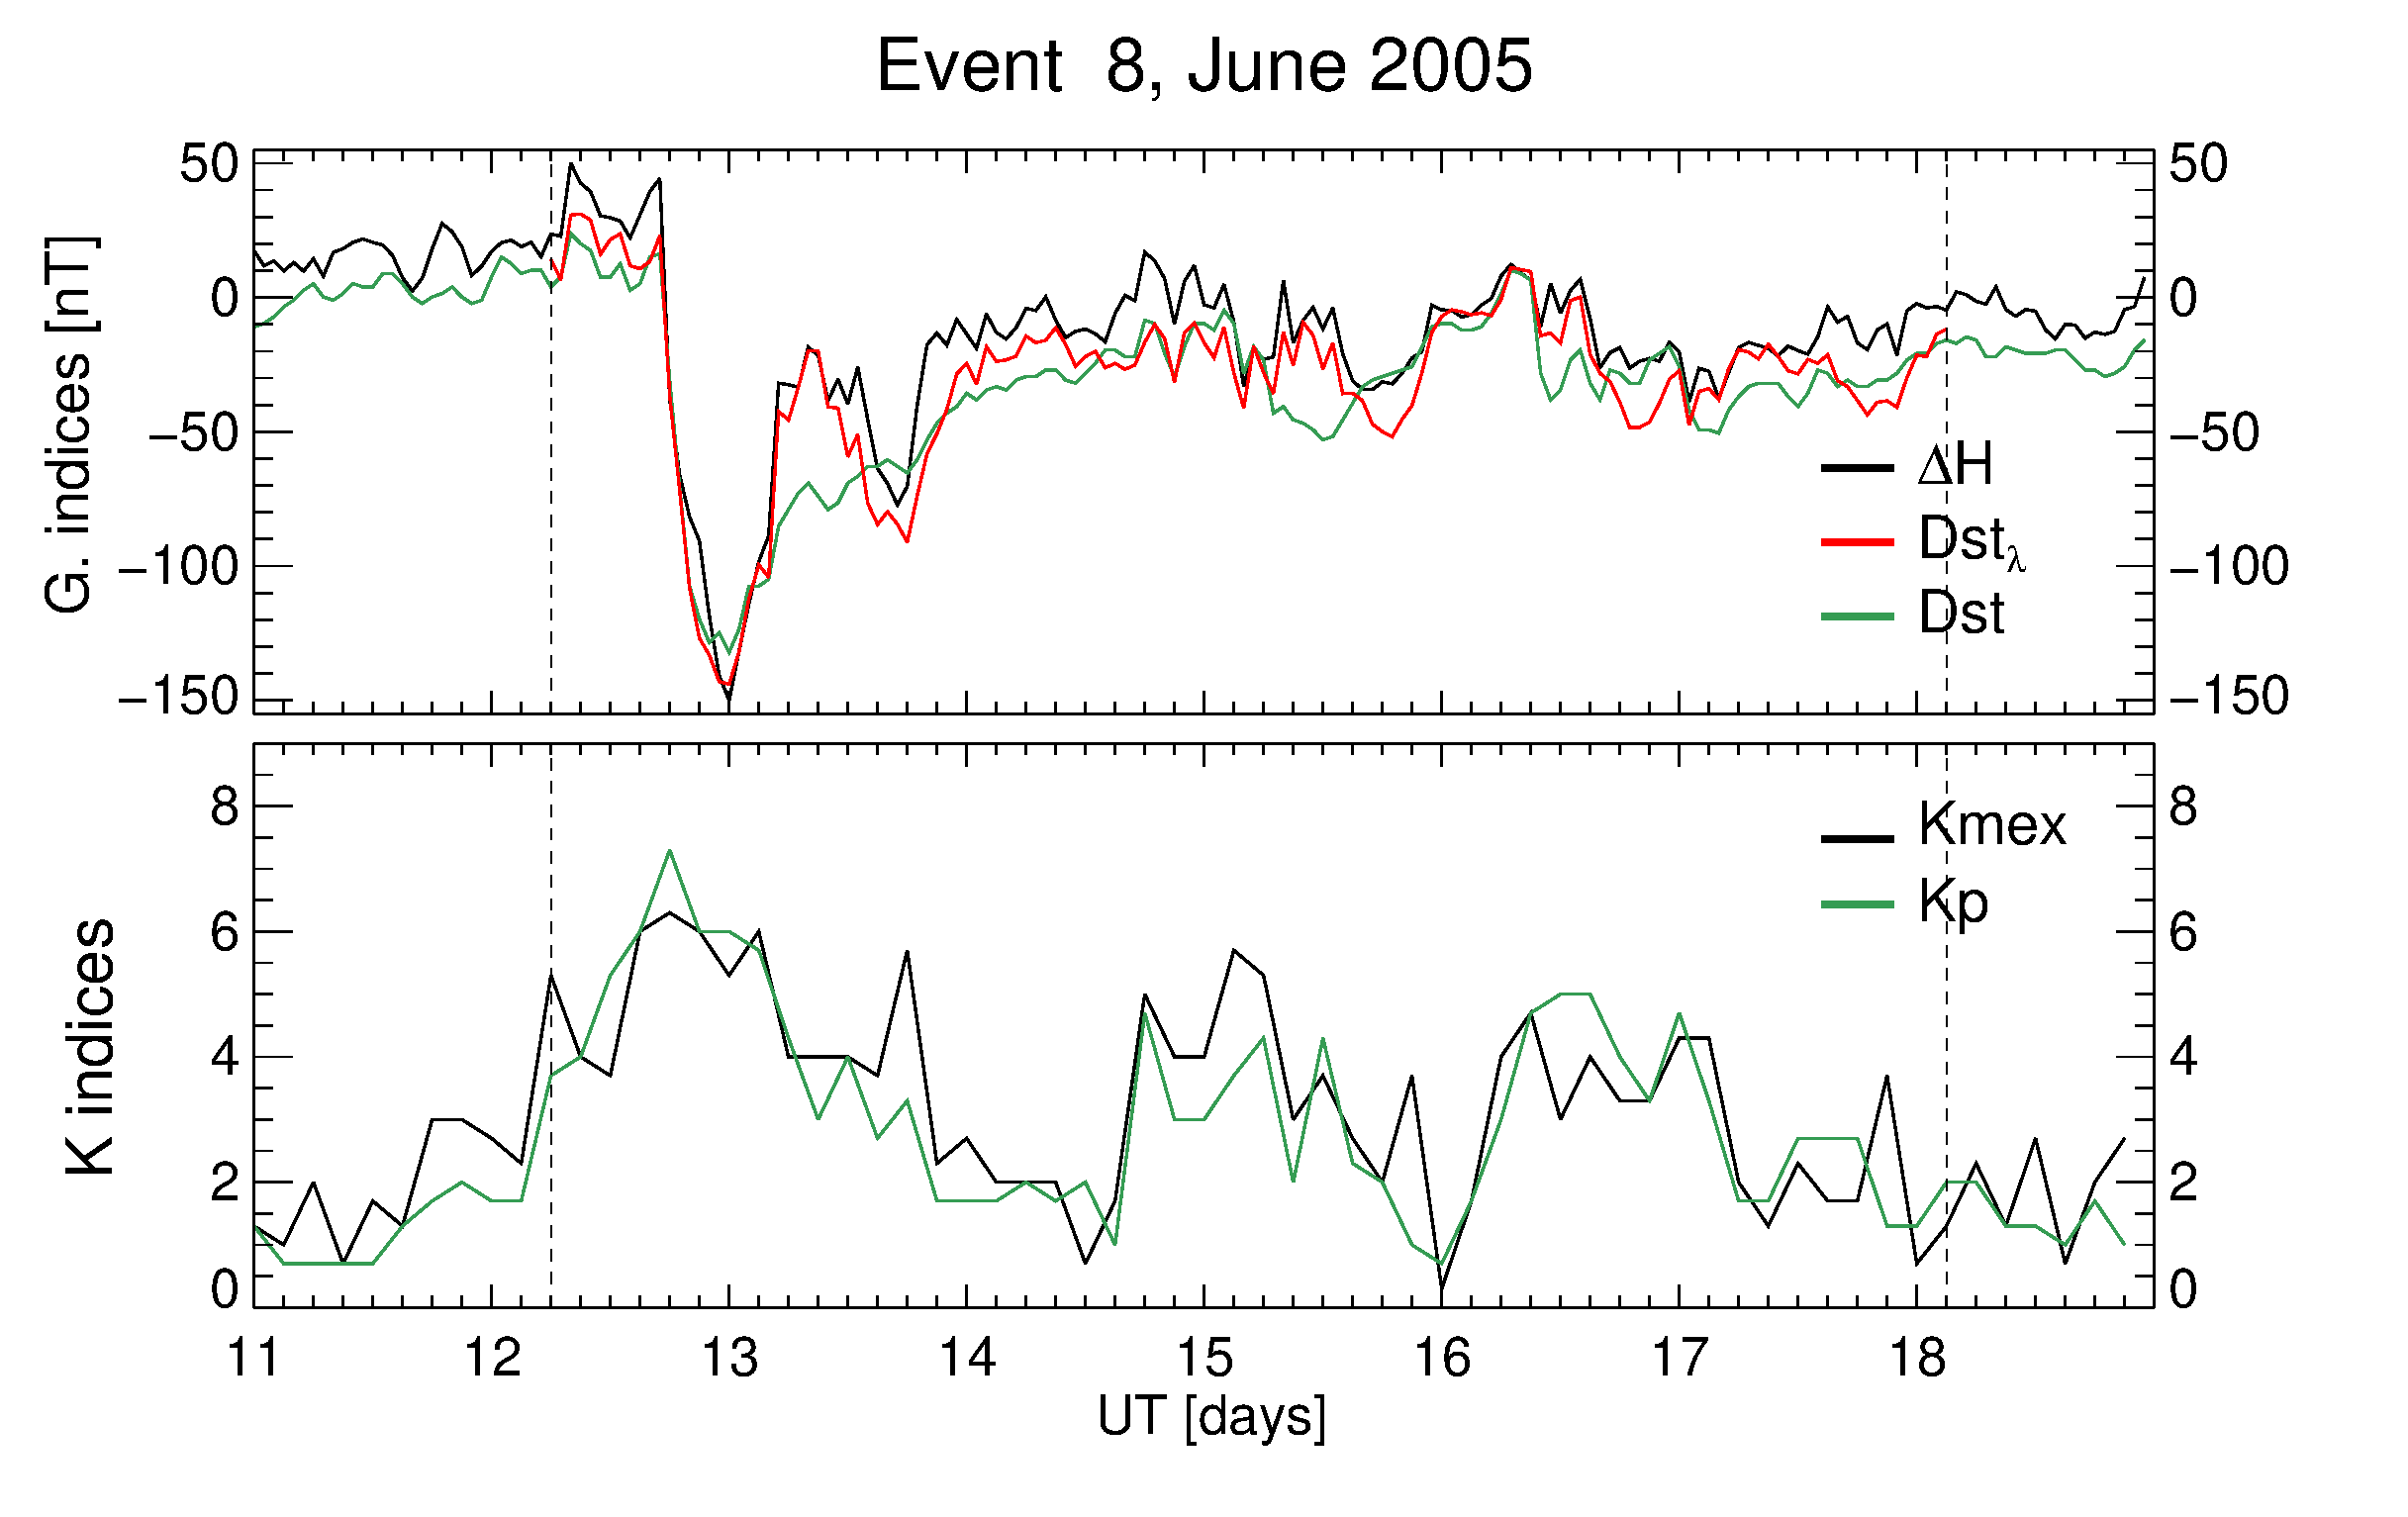
\includegraphics[width=6.0cm]{images/dH_approx/diono_valid_V4_2005-06-11.eps}     
       \centerline{\Large \bf   
      \hspace{0.275\textwidth}  \color{black}{}
       \hspace{0.295\textwidth}  \color{black}{}
         \hfill}
	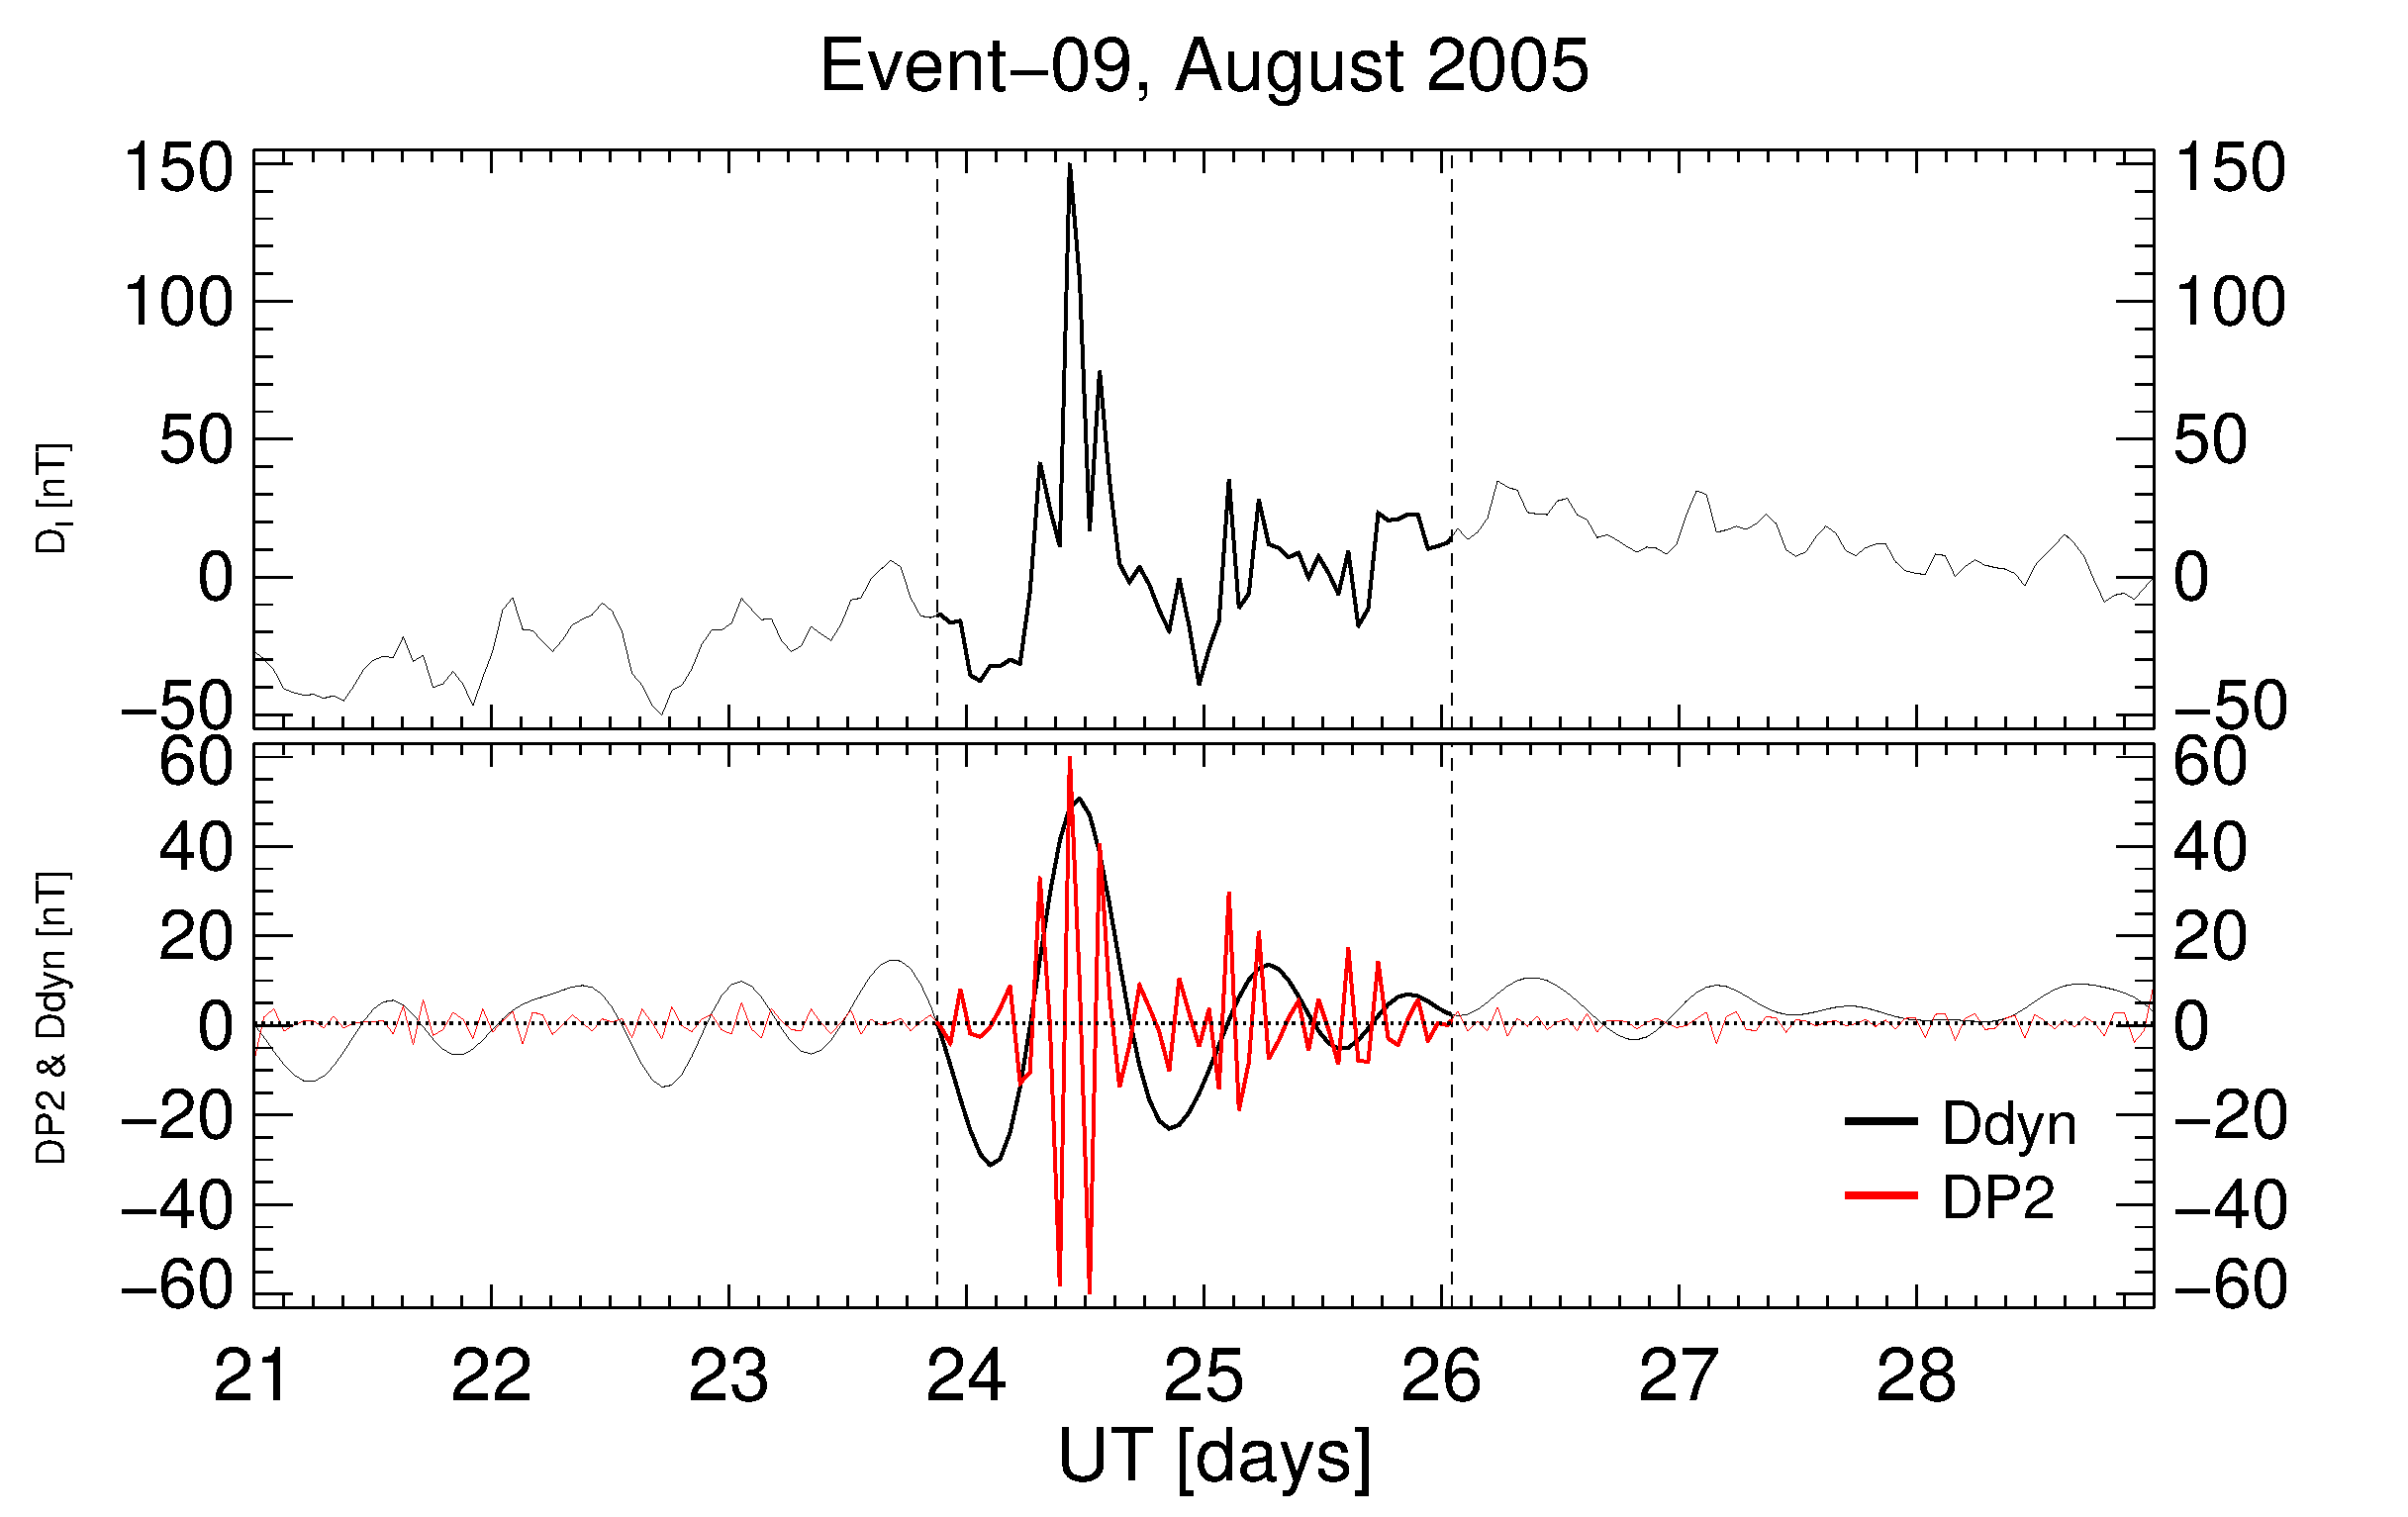
\includegraphics[width=6.0cm]{images/diono/iono_PI_V1_2005-08-21.eps}   
    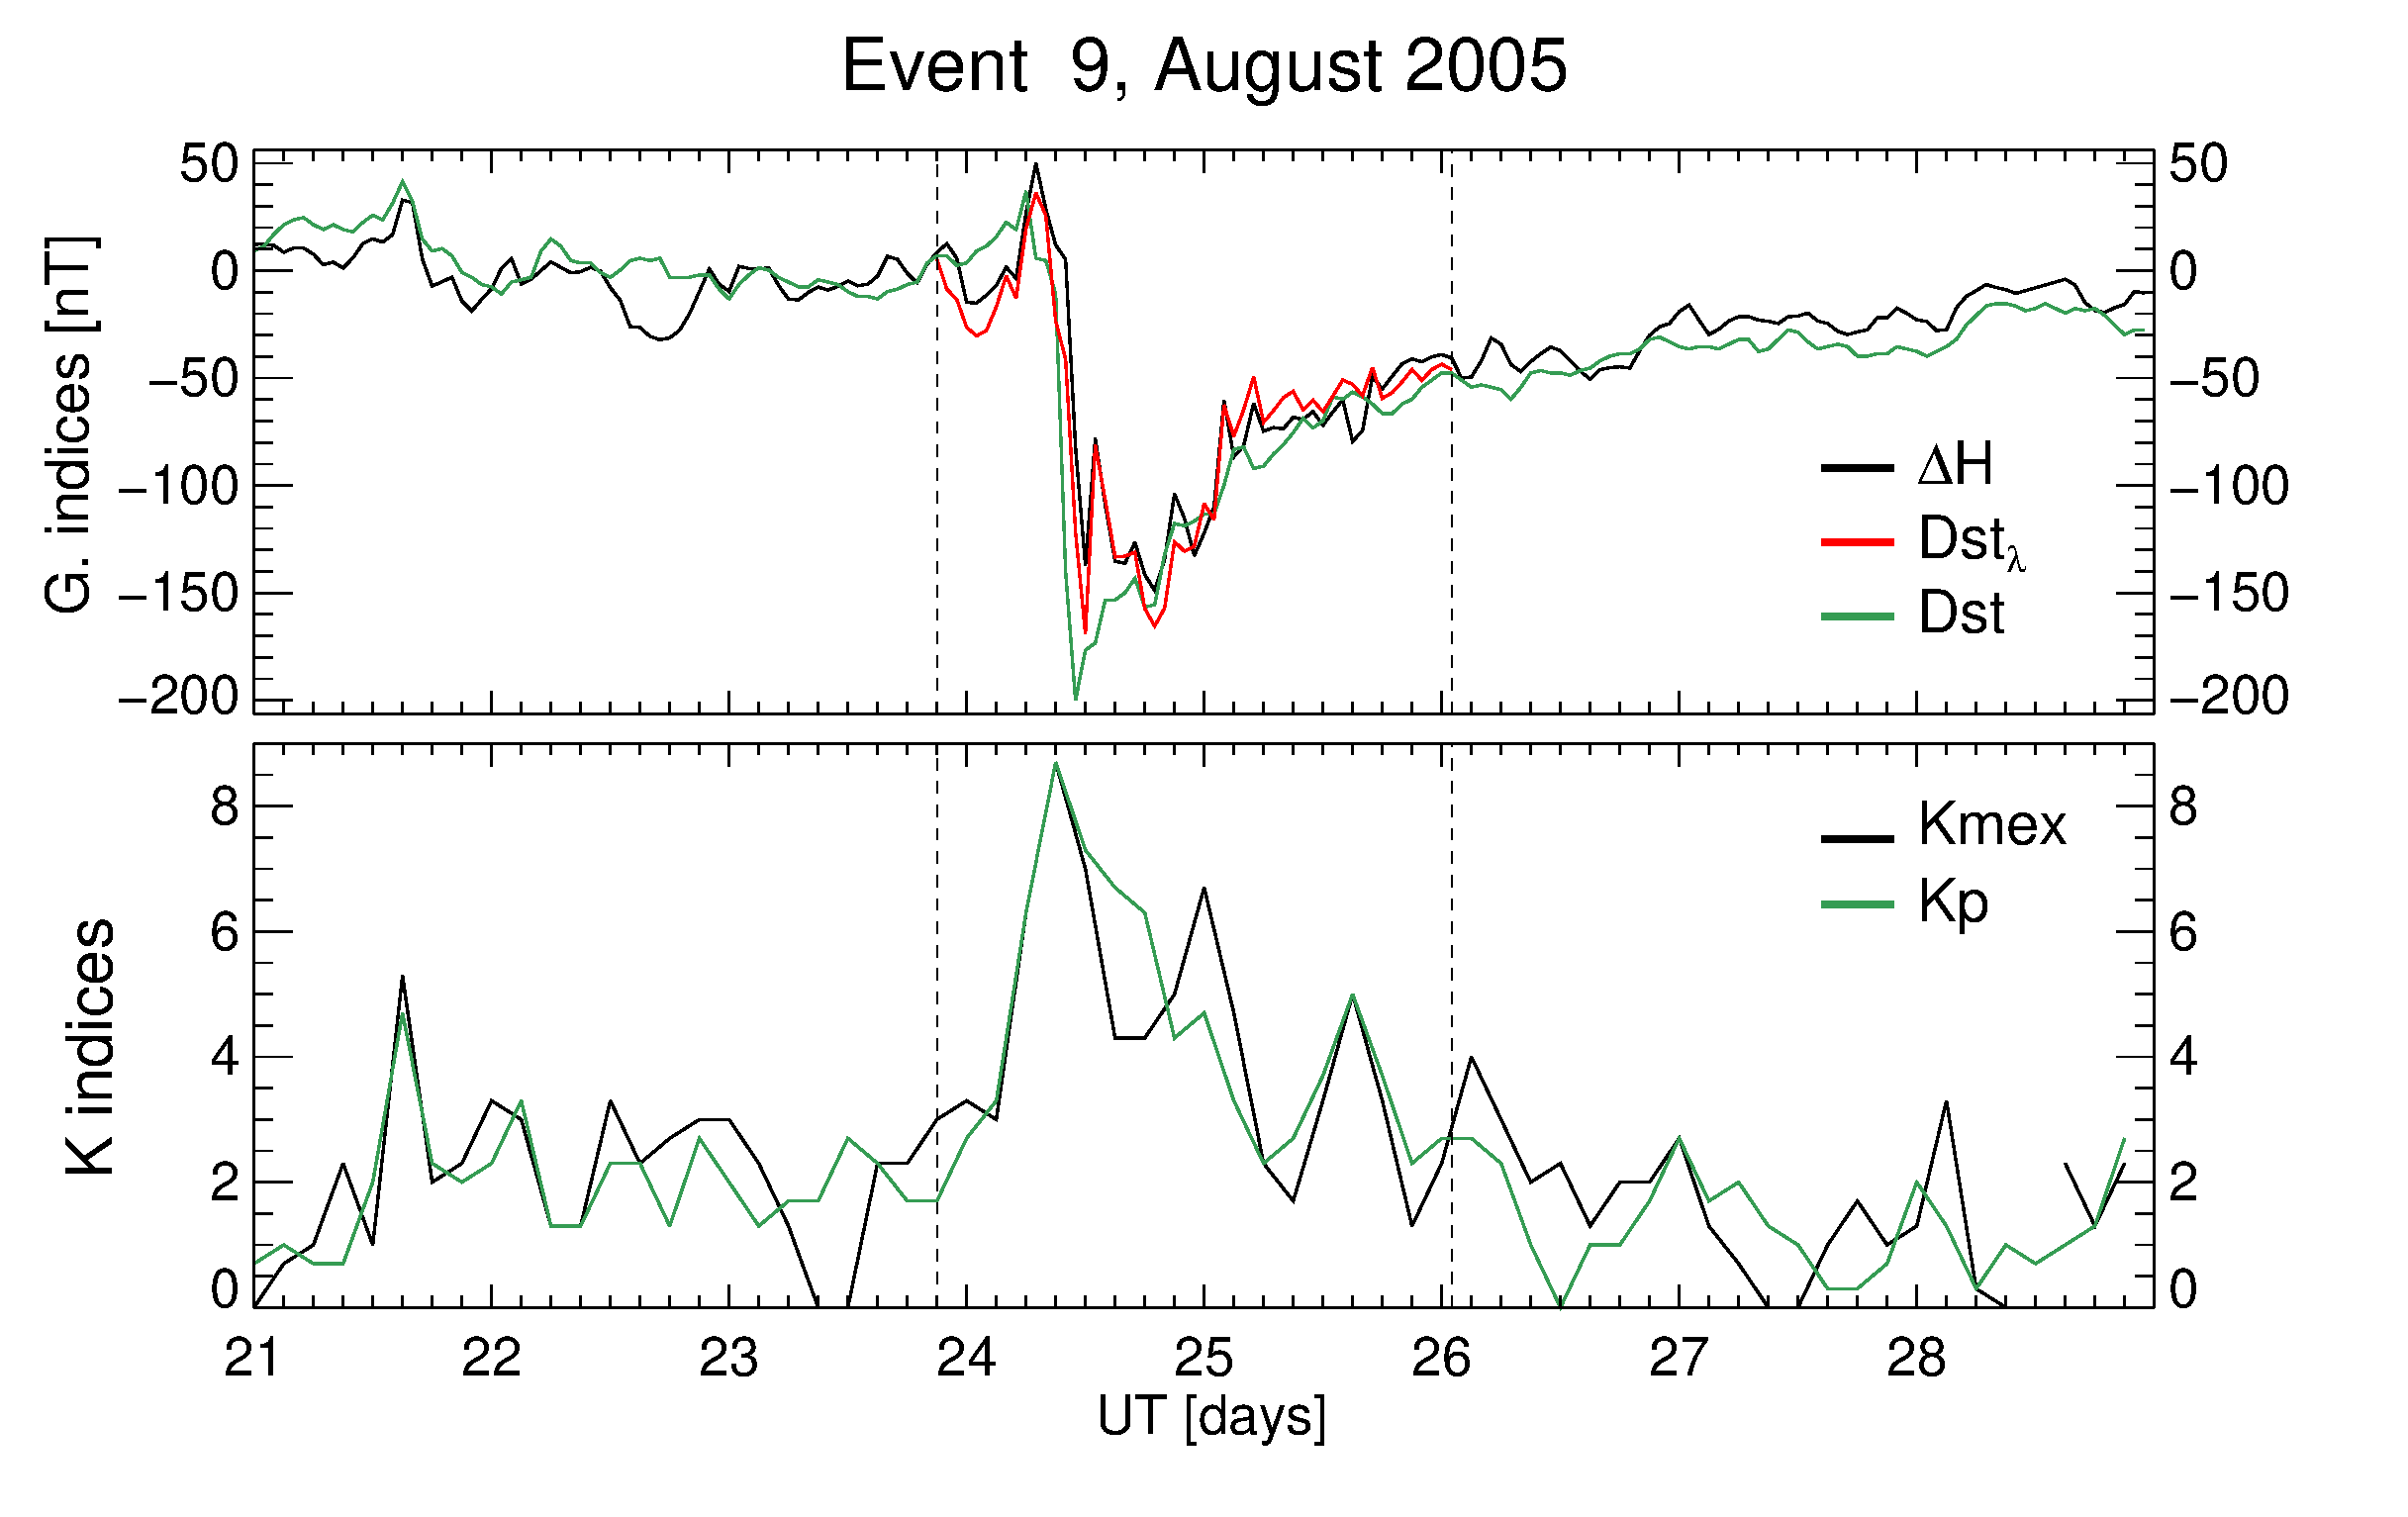
\includegraphics[width=6.0cm]{images/dH_approx/diono_valid_V4_2005-08-21.eps}     

       \centerline{\Large \bf   
      \hspace{0.275\textwidth}  \color{black}{}
       \hspace{0.295\textwidth}  \color{black}{}
         \hfill}
	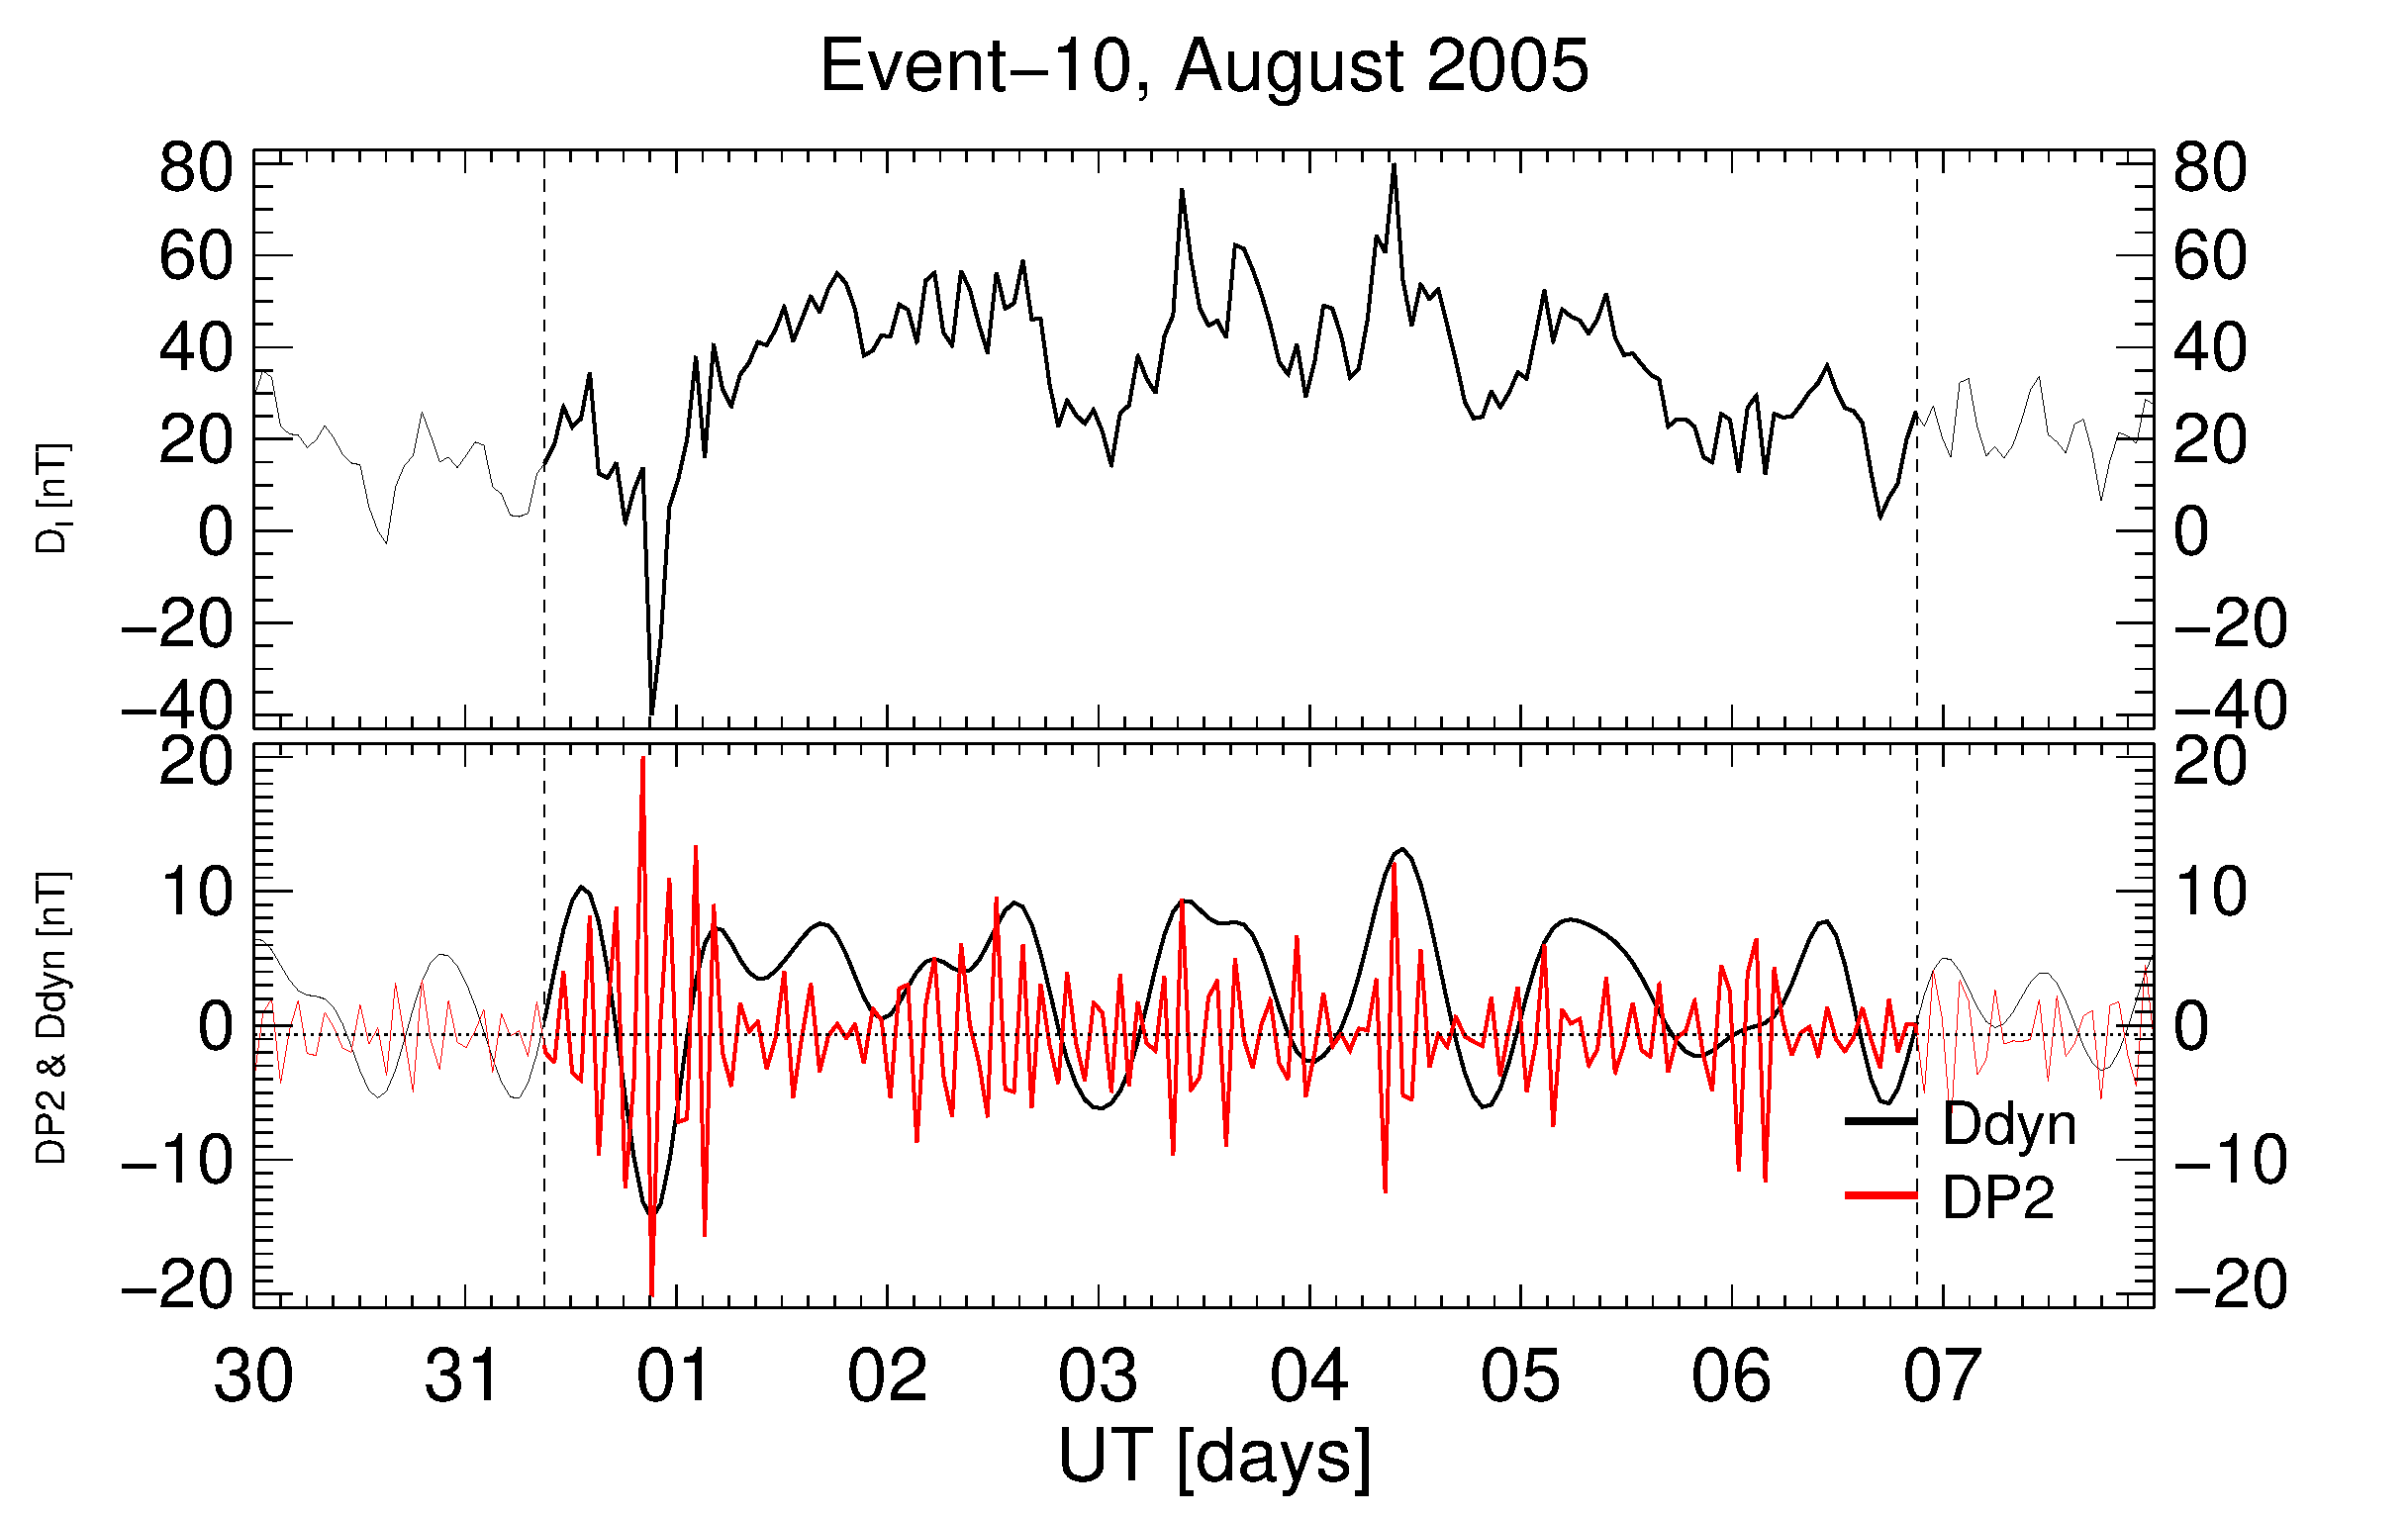
\includegraphics[width=6.0cm]{images/diono/iono_PI_V1_2005-08-30.eps}
	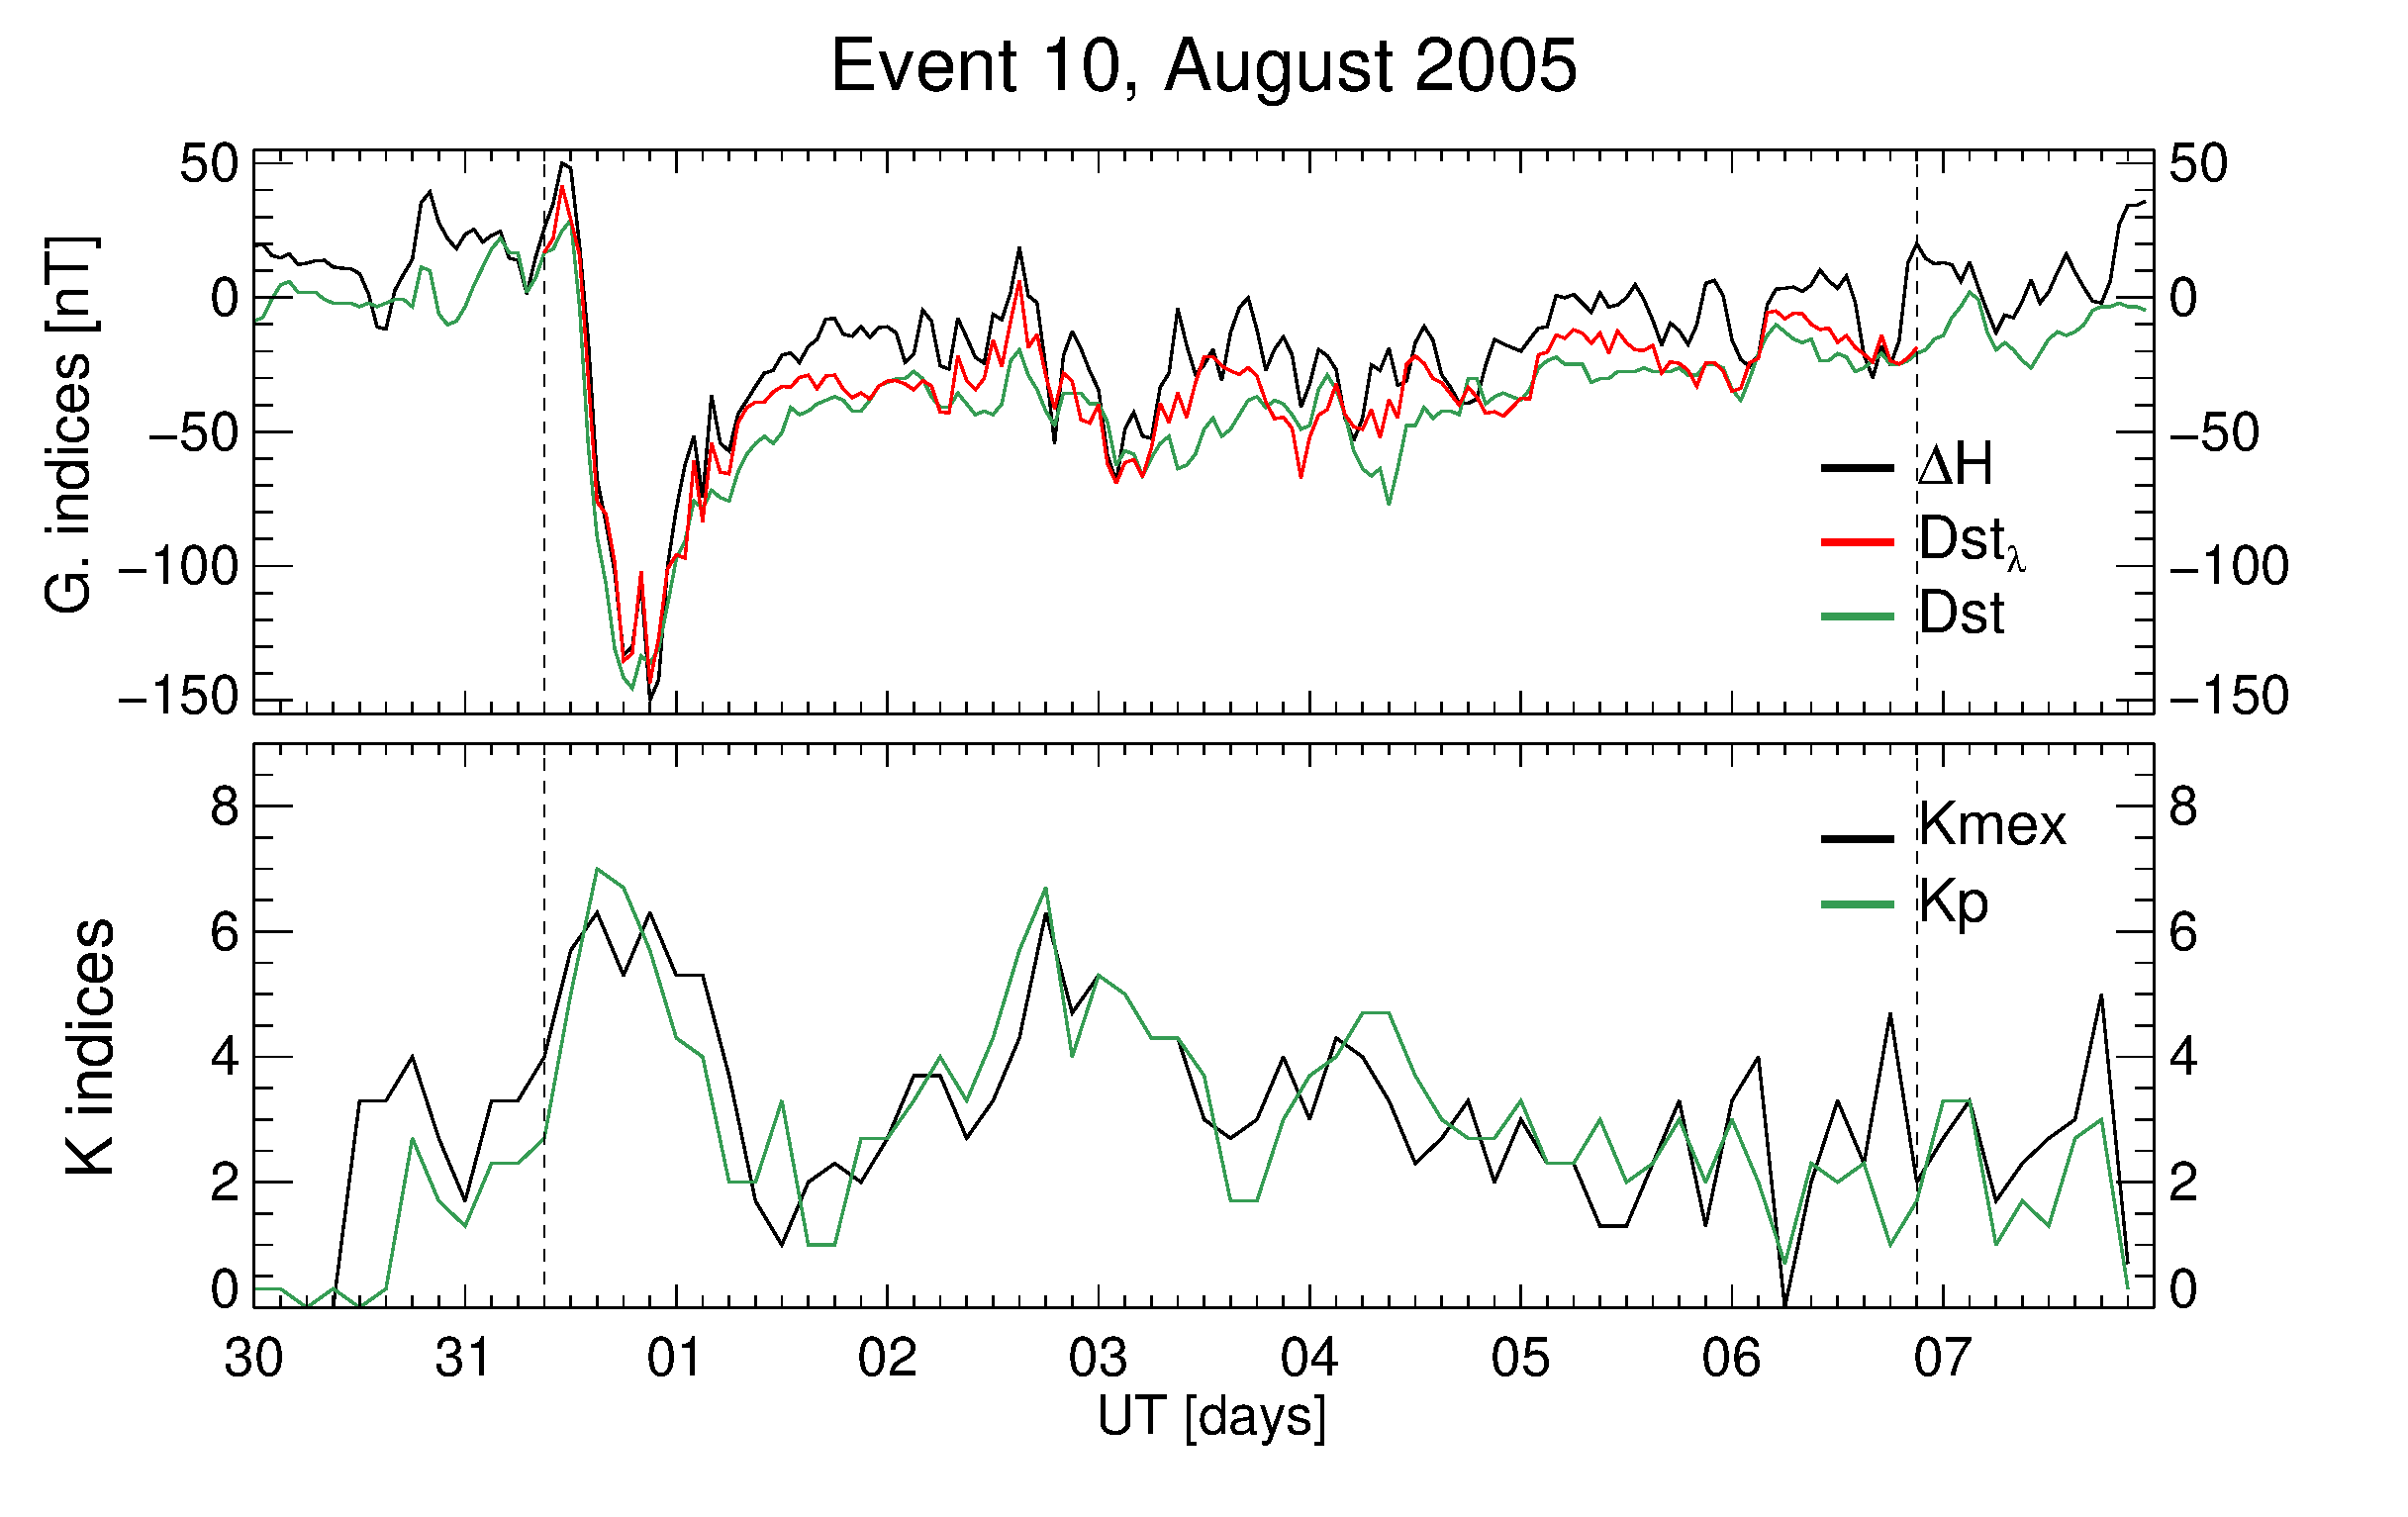
\includegraphics[width=6.0cm]{images/dH_approx/diono_valid_V4_2005-08-30.eps}	
       
       \caption{On the right side, top panels illustrate the contribution of Ionospheric Magnetic Disturbances, while bottom panels depict the isolated geomagnetic contributions of $Ddyn$ and $DP2$. The vertical dashed lines highlight the geomagnetic storm time period during which such calculations are valid. On the left side, green lines represent planetary indices, while black lines denote local indices. Additionally, red lines represent the approximation of $\Delta H$ at top, while bottom showcases the comparison of local $K$ (black line) and planetary $K$ (green line).
       }
    \label{fig:iono_resp3}
\end{figure*}


\begin{figure*}[h!]
    \centering
    \centerline{\Large \bf   
      %\hspace{0.18\textwidth}  \color{black}{\Large{Res}}
       %\hspace{0.28\textwidth}  \color{black}{\Large{Res+TC}}
         \hfill}
          \centerline{\Large \bf   
      \hspace{0.26\textwidth}  \color{black}{}
       \hspace{0.31\textwidth}  \color{black}{}
         \hfill}
     \centerline{\Large \bf   
      \hspace{0.275\textwidth}  \color{black}{}
       \hspace{0.295\textwidth}  \color{black}{}
         \hfill}
	 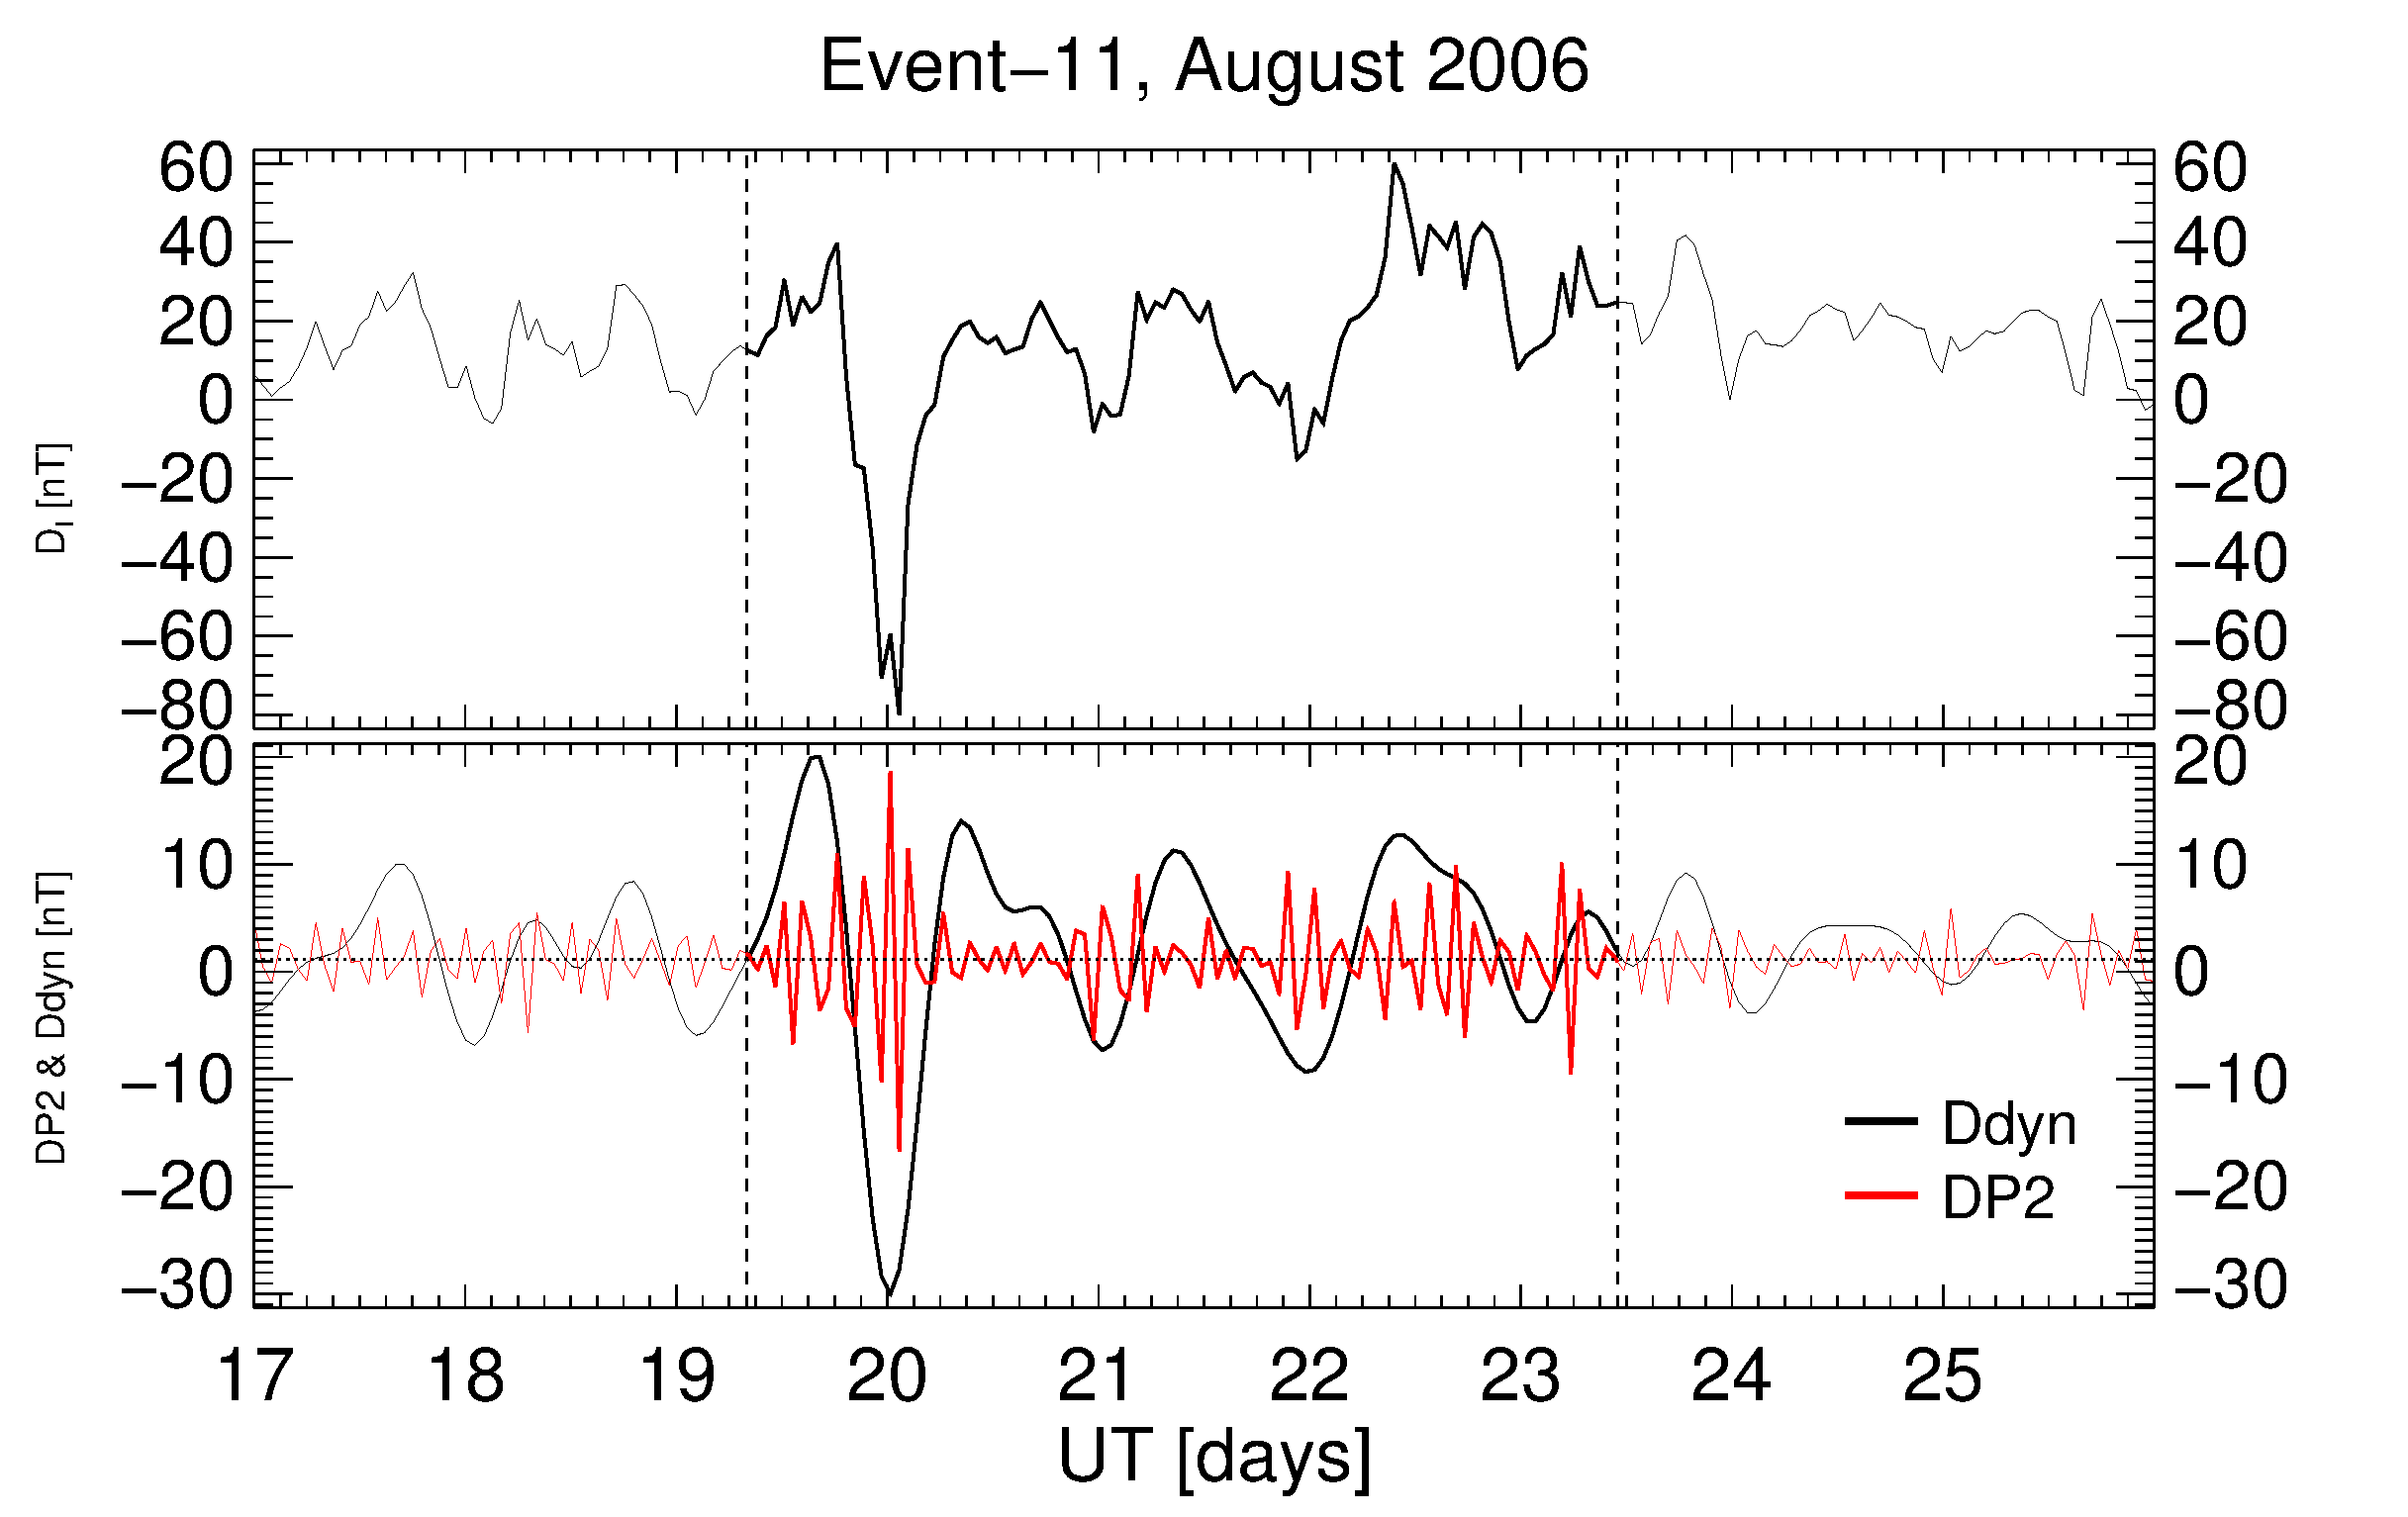
\includegraphics[width=6.0cm]{images/diono/iono_PI_V1_2006-08-17.eps}
     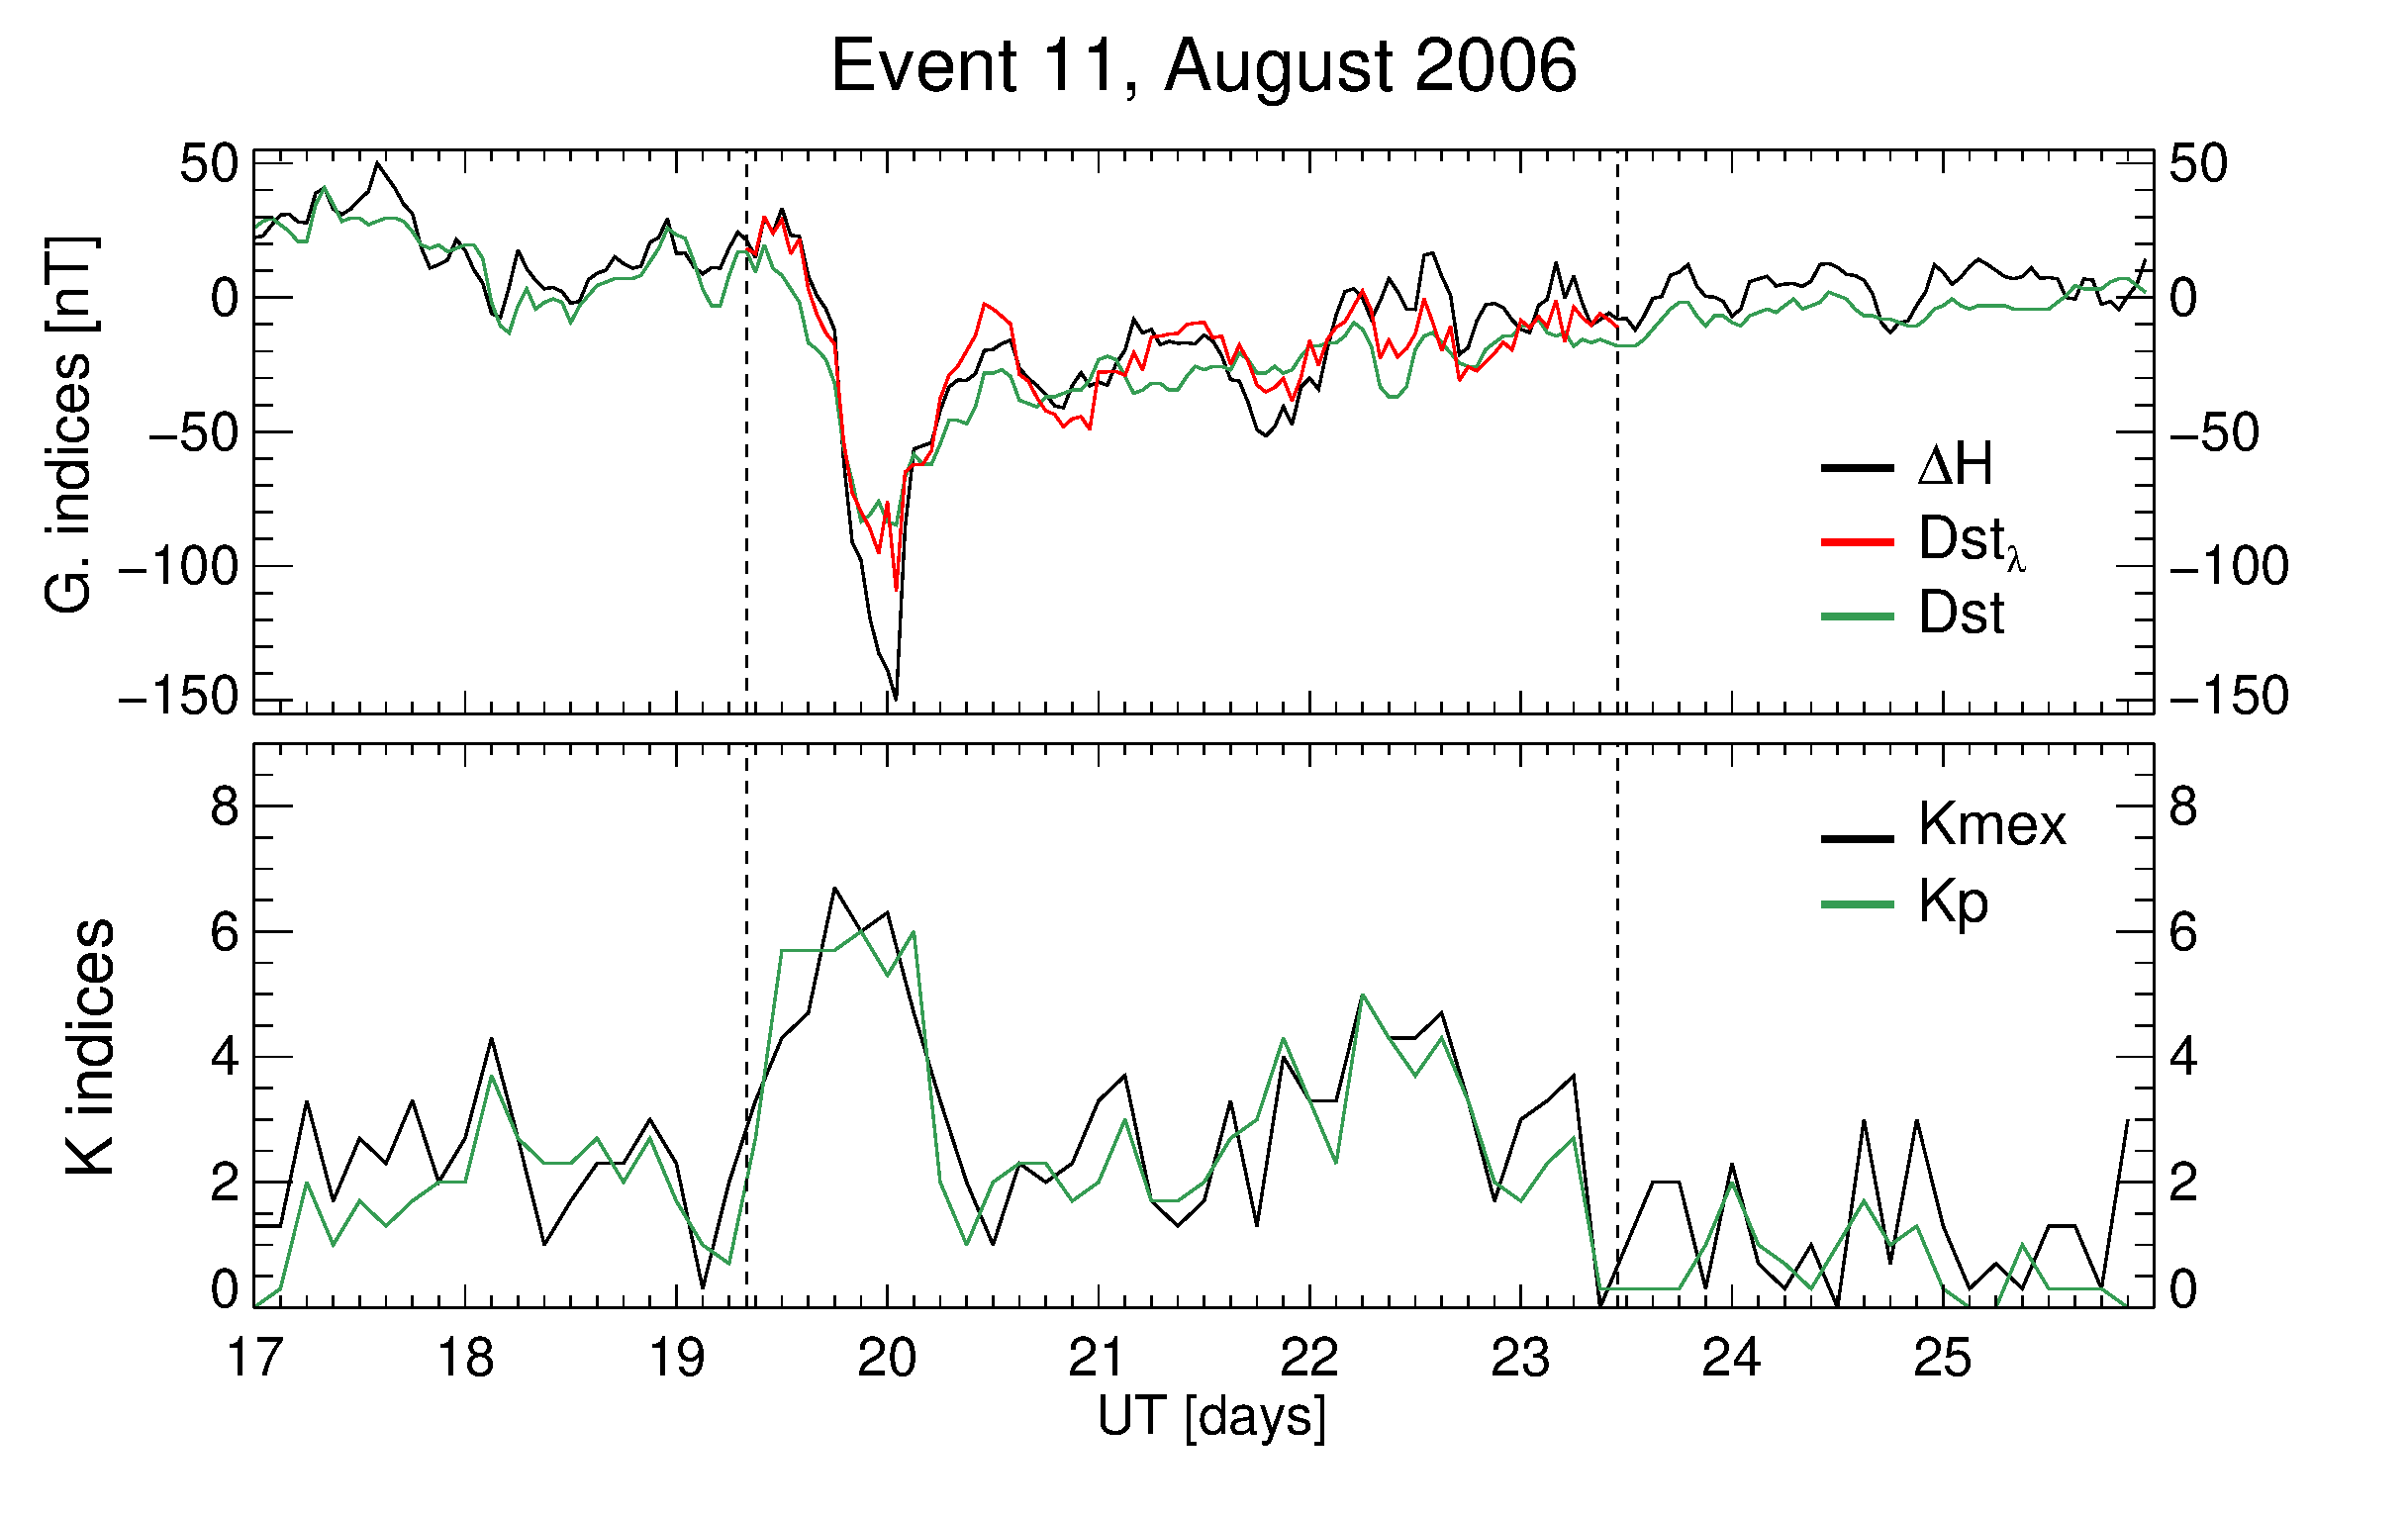
\includegraphics[width=6.0cm]{images/dH_approx/diono_valid_V4_2006-08-17.eps}	
     \centerline{\Large \bf   
      \hspace{0.275\textwidth}  \color{black}{}
       \hspace{0.295\textwidth}  \color{black}{}
         \hfill}
     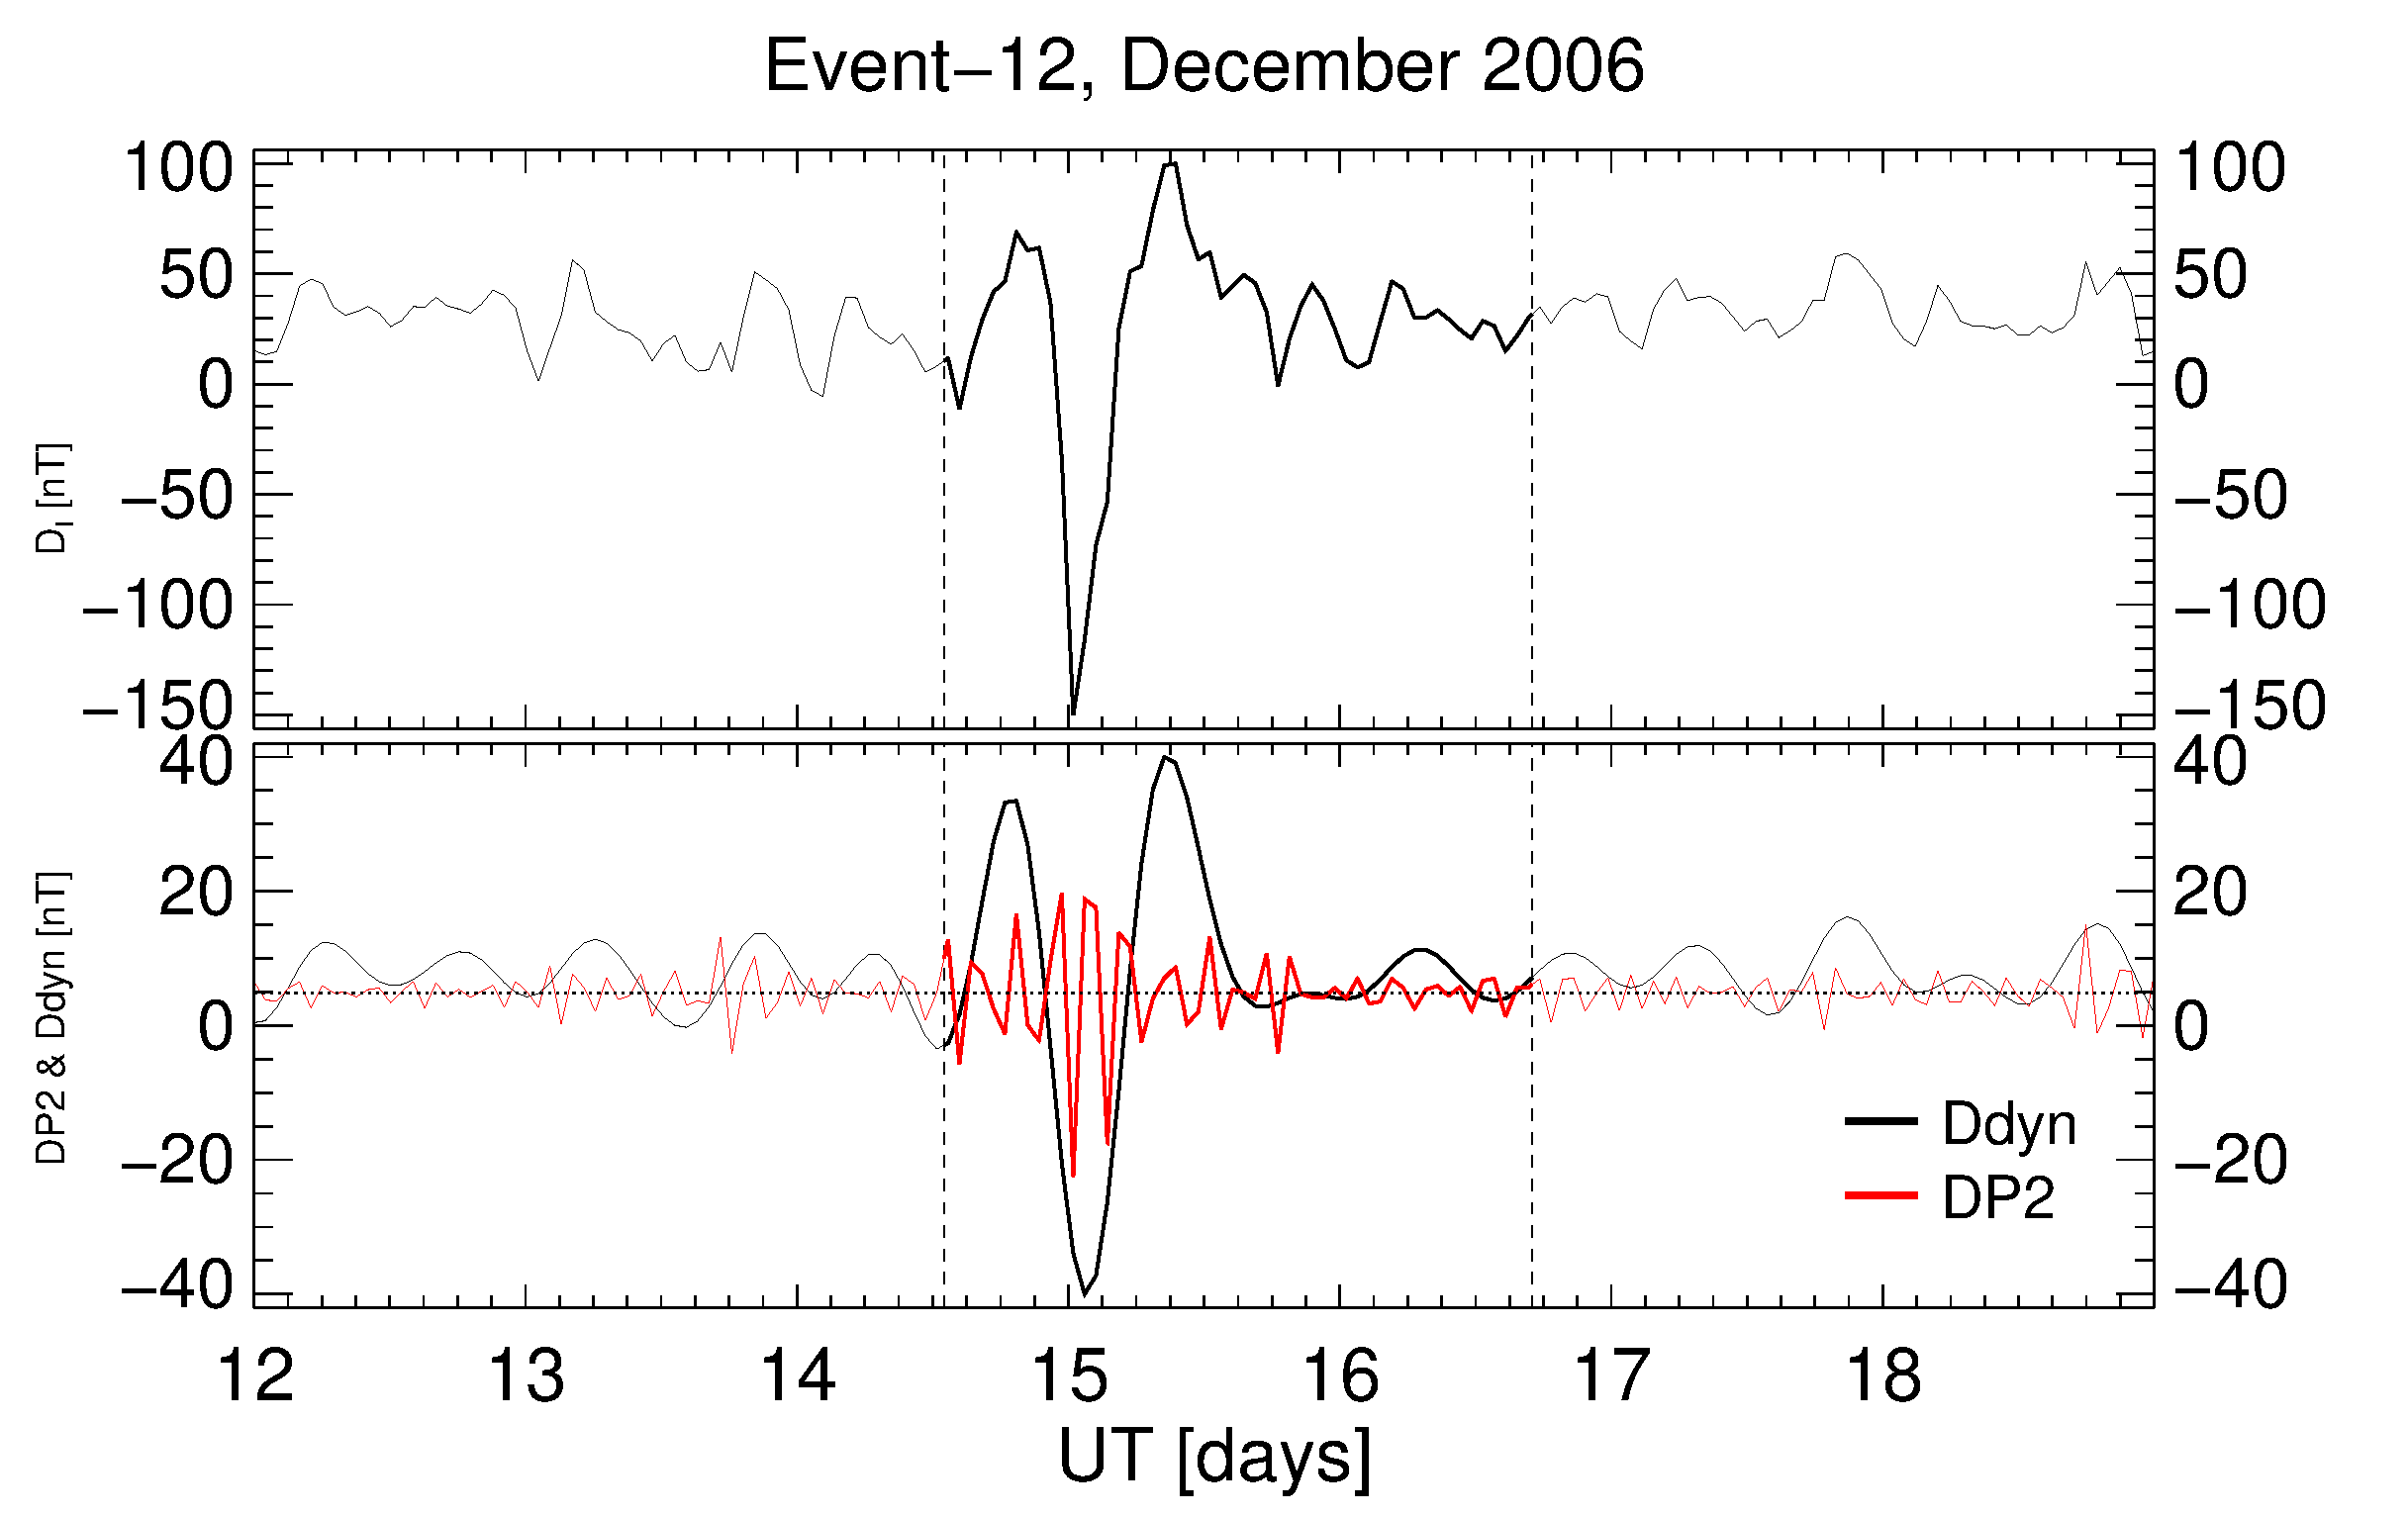
\includegraphics[width=6.0cm]{images/diono/iono_PI_V1_2006-12-12.eps}
     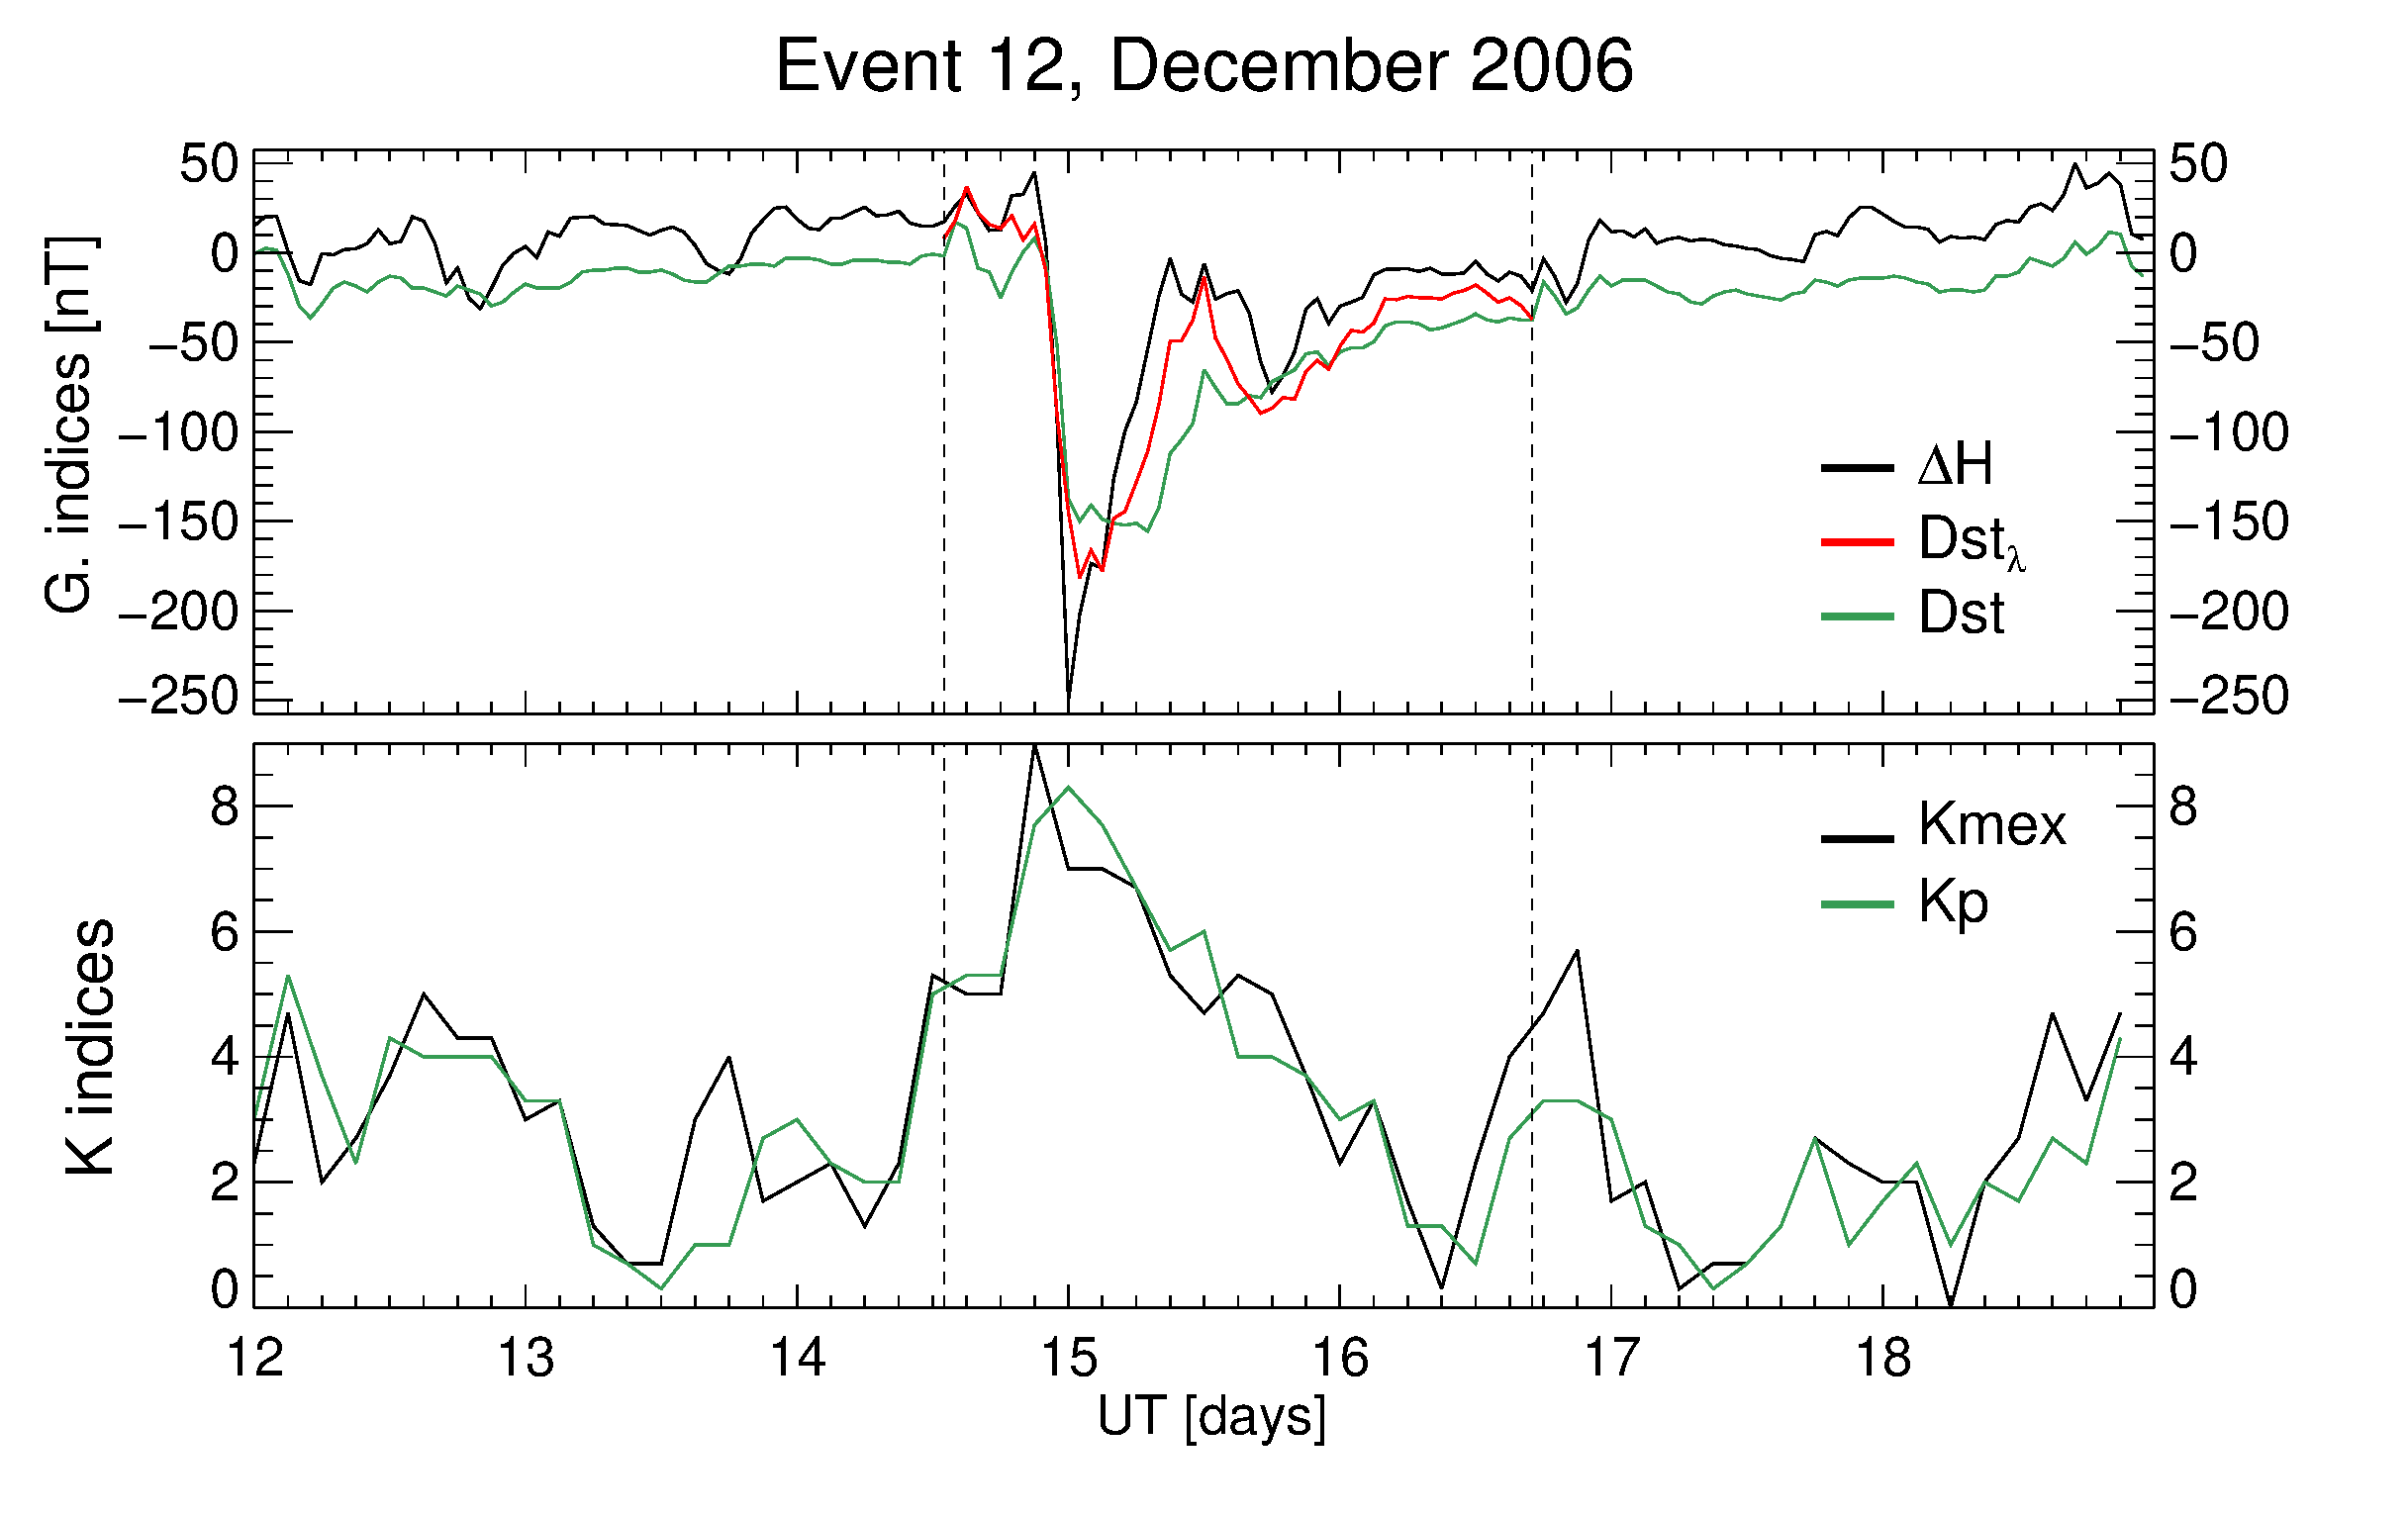
\includegraphics[width=6.0cm]{images/dH_approx/diono_valid_V4_2006-12-12.eps}     
       \centerline{\Large \bf   
      \hspace{0.275\textwidth}  \color{black}{}
       \hspace{0.295\textwidth}  \color{black}{}
         \hfill}
	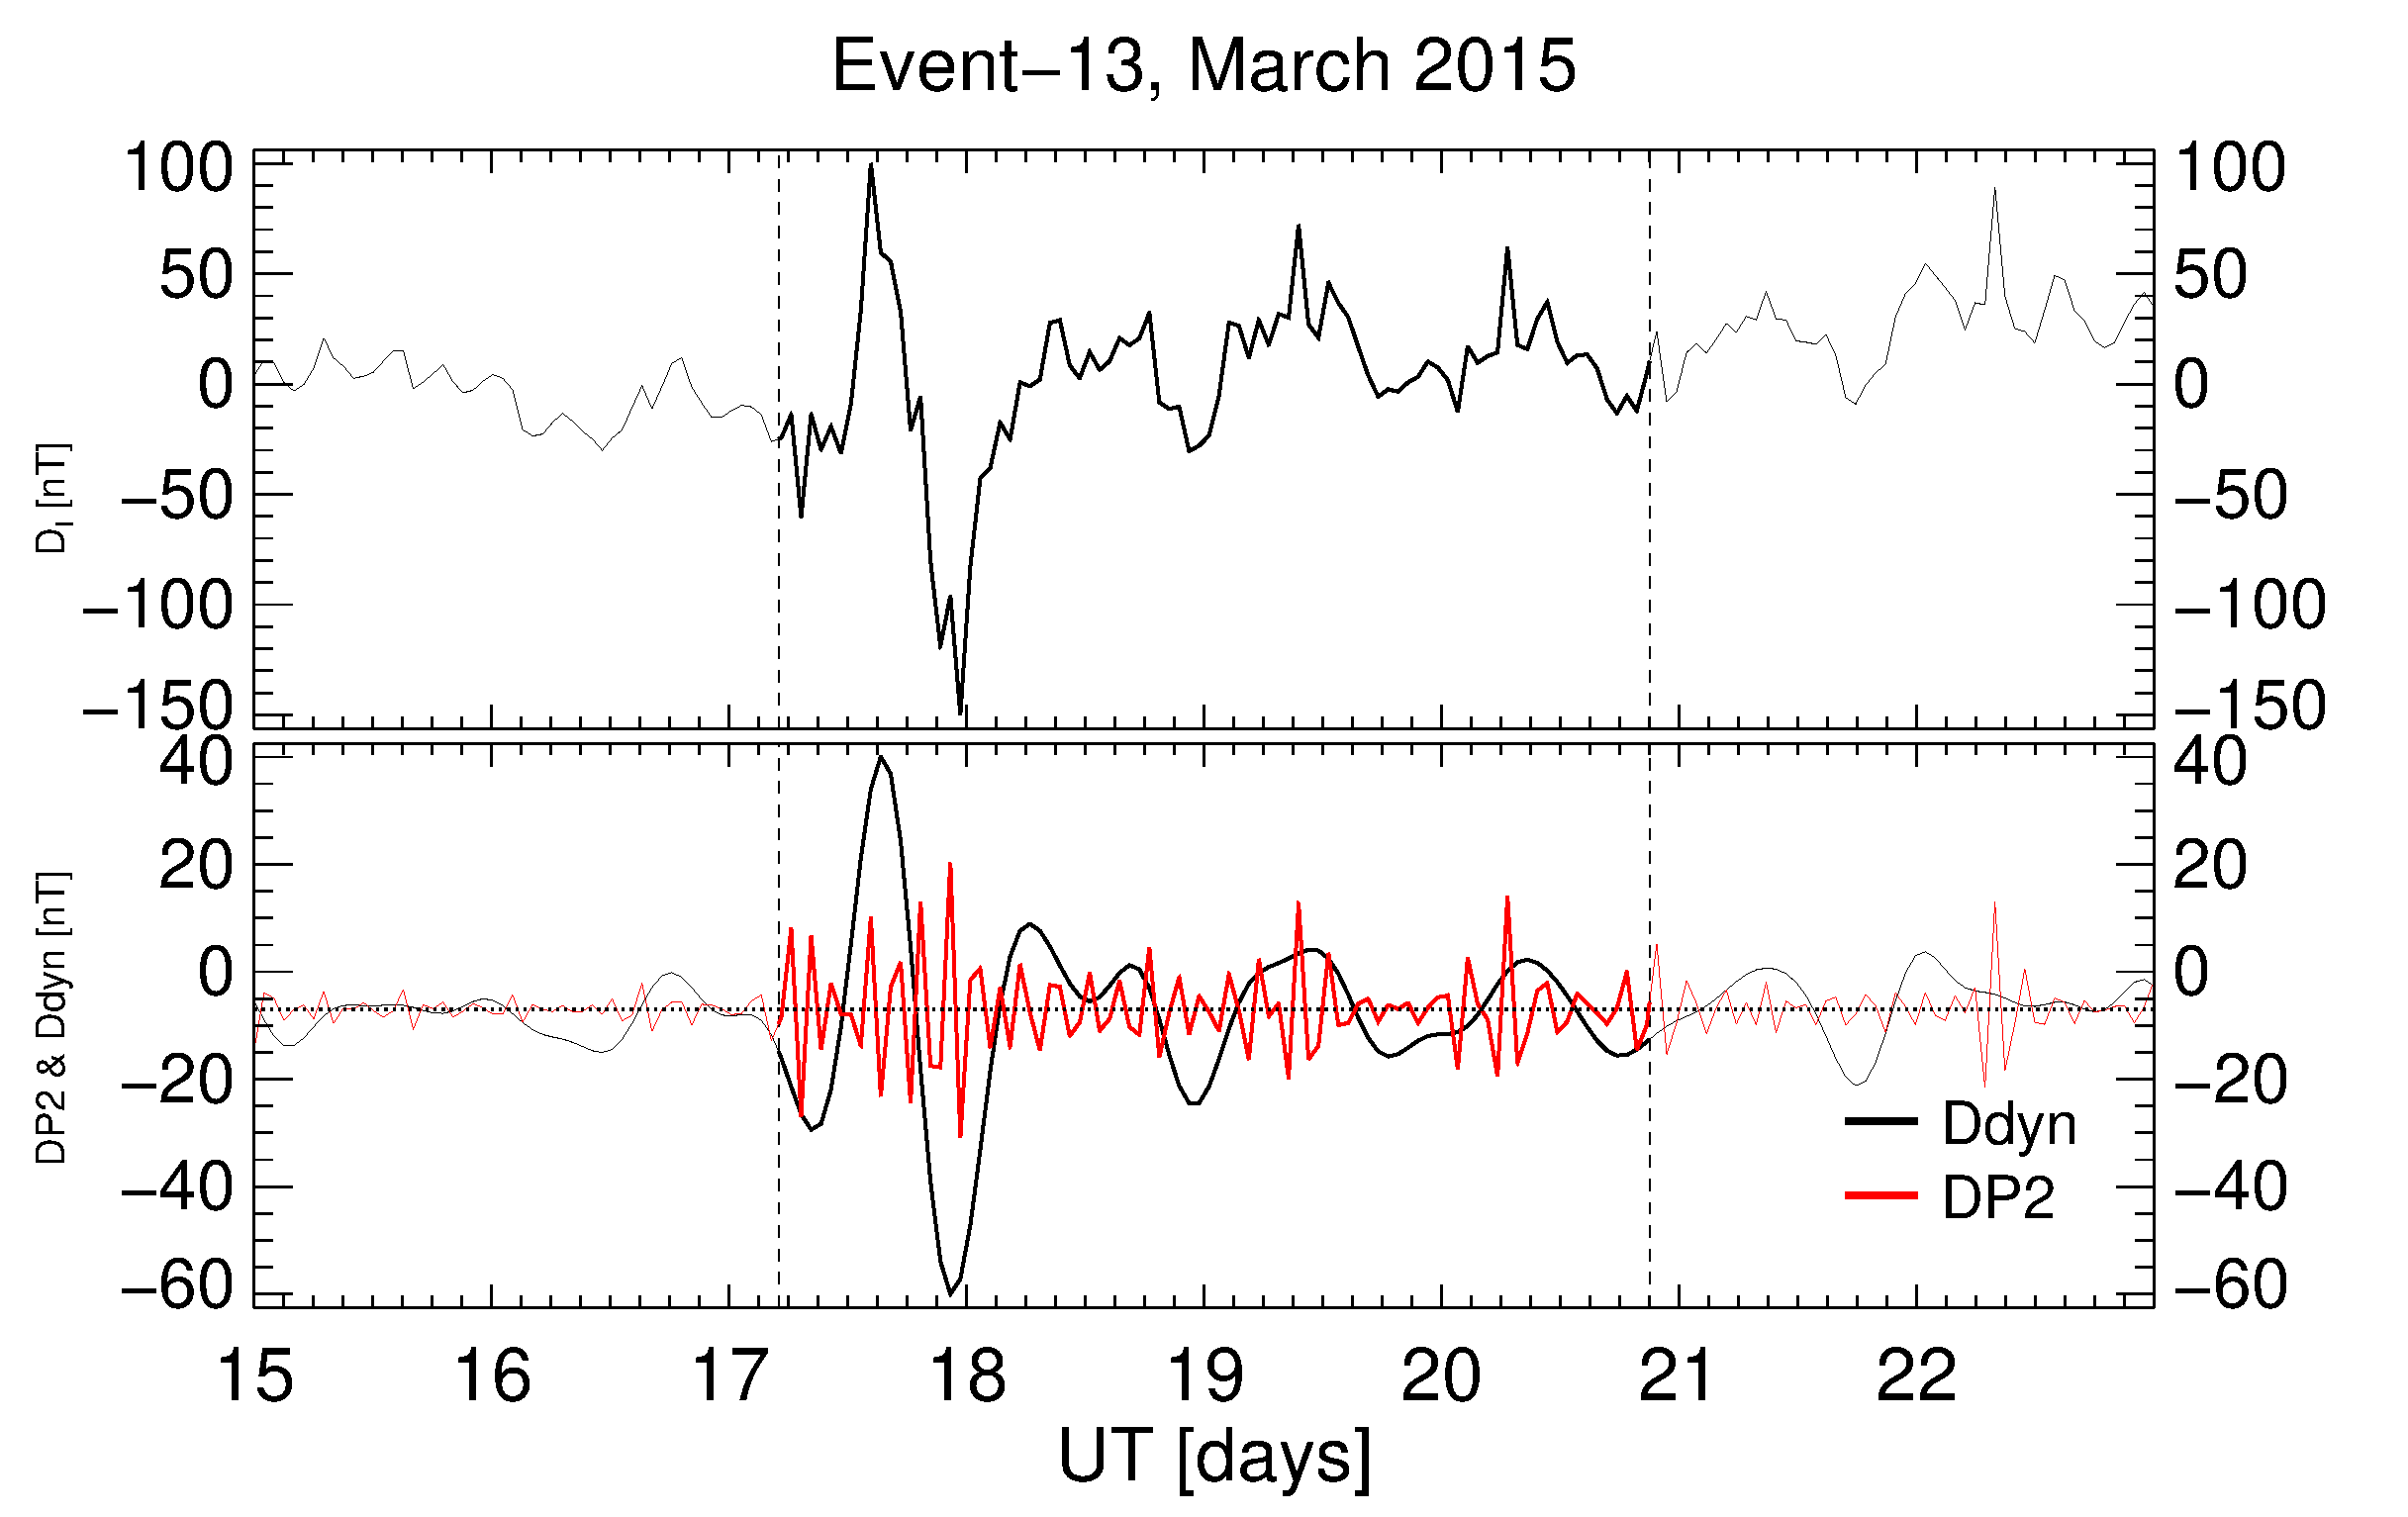
\includegraphics[width=6.0cm]{images/diono/iono_PI_V1_2015-03-15.eps}    
    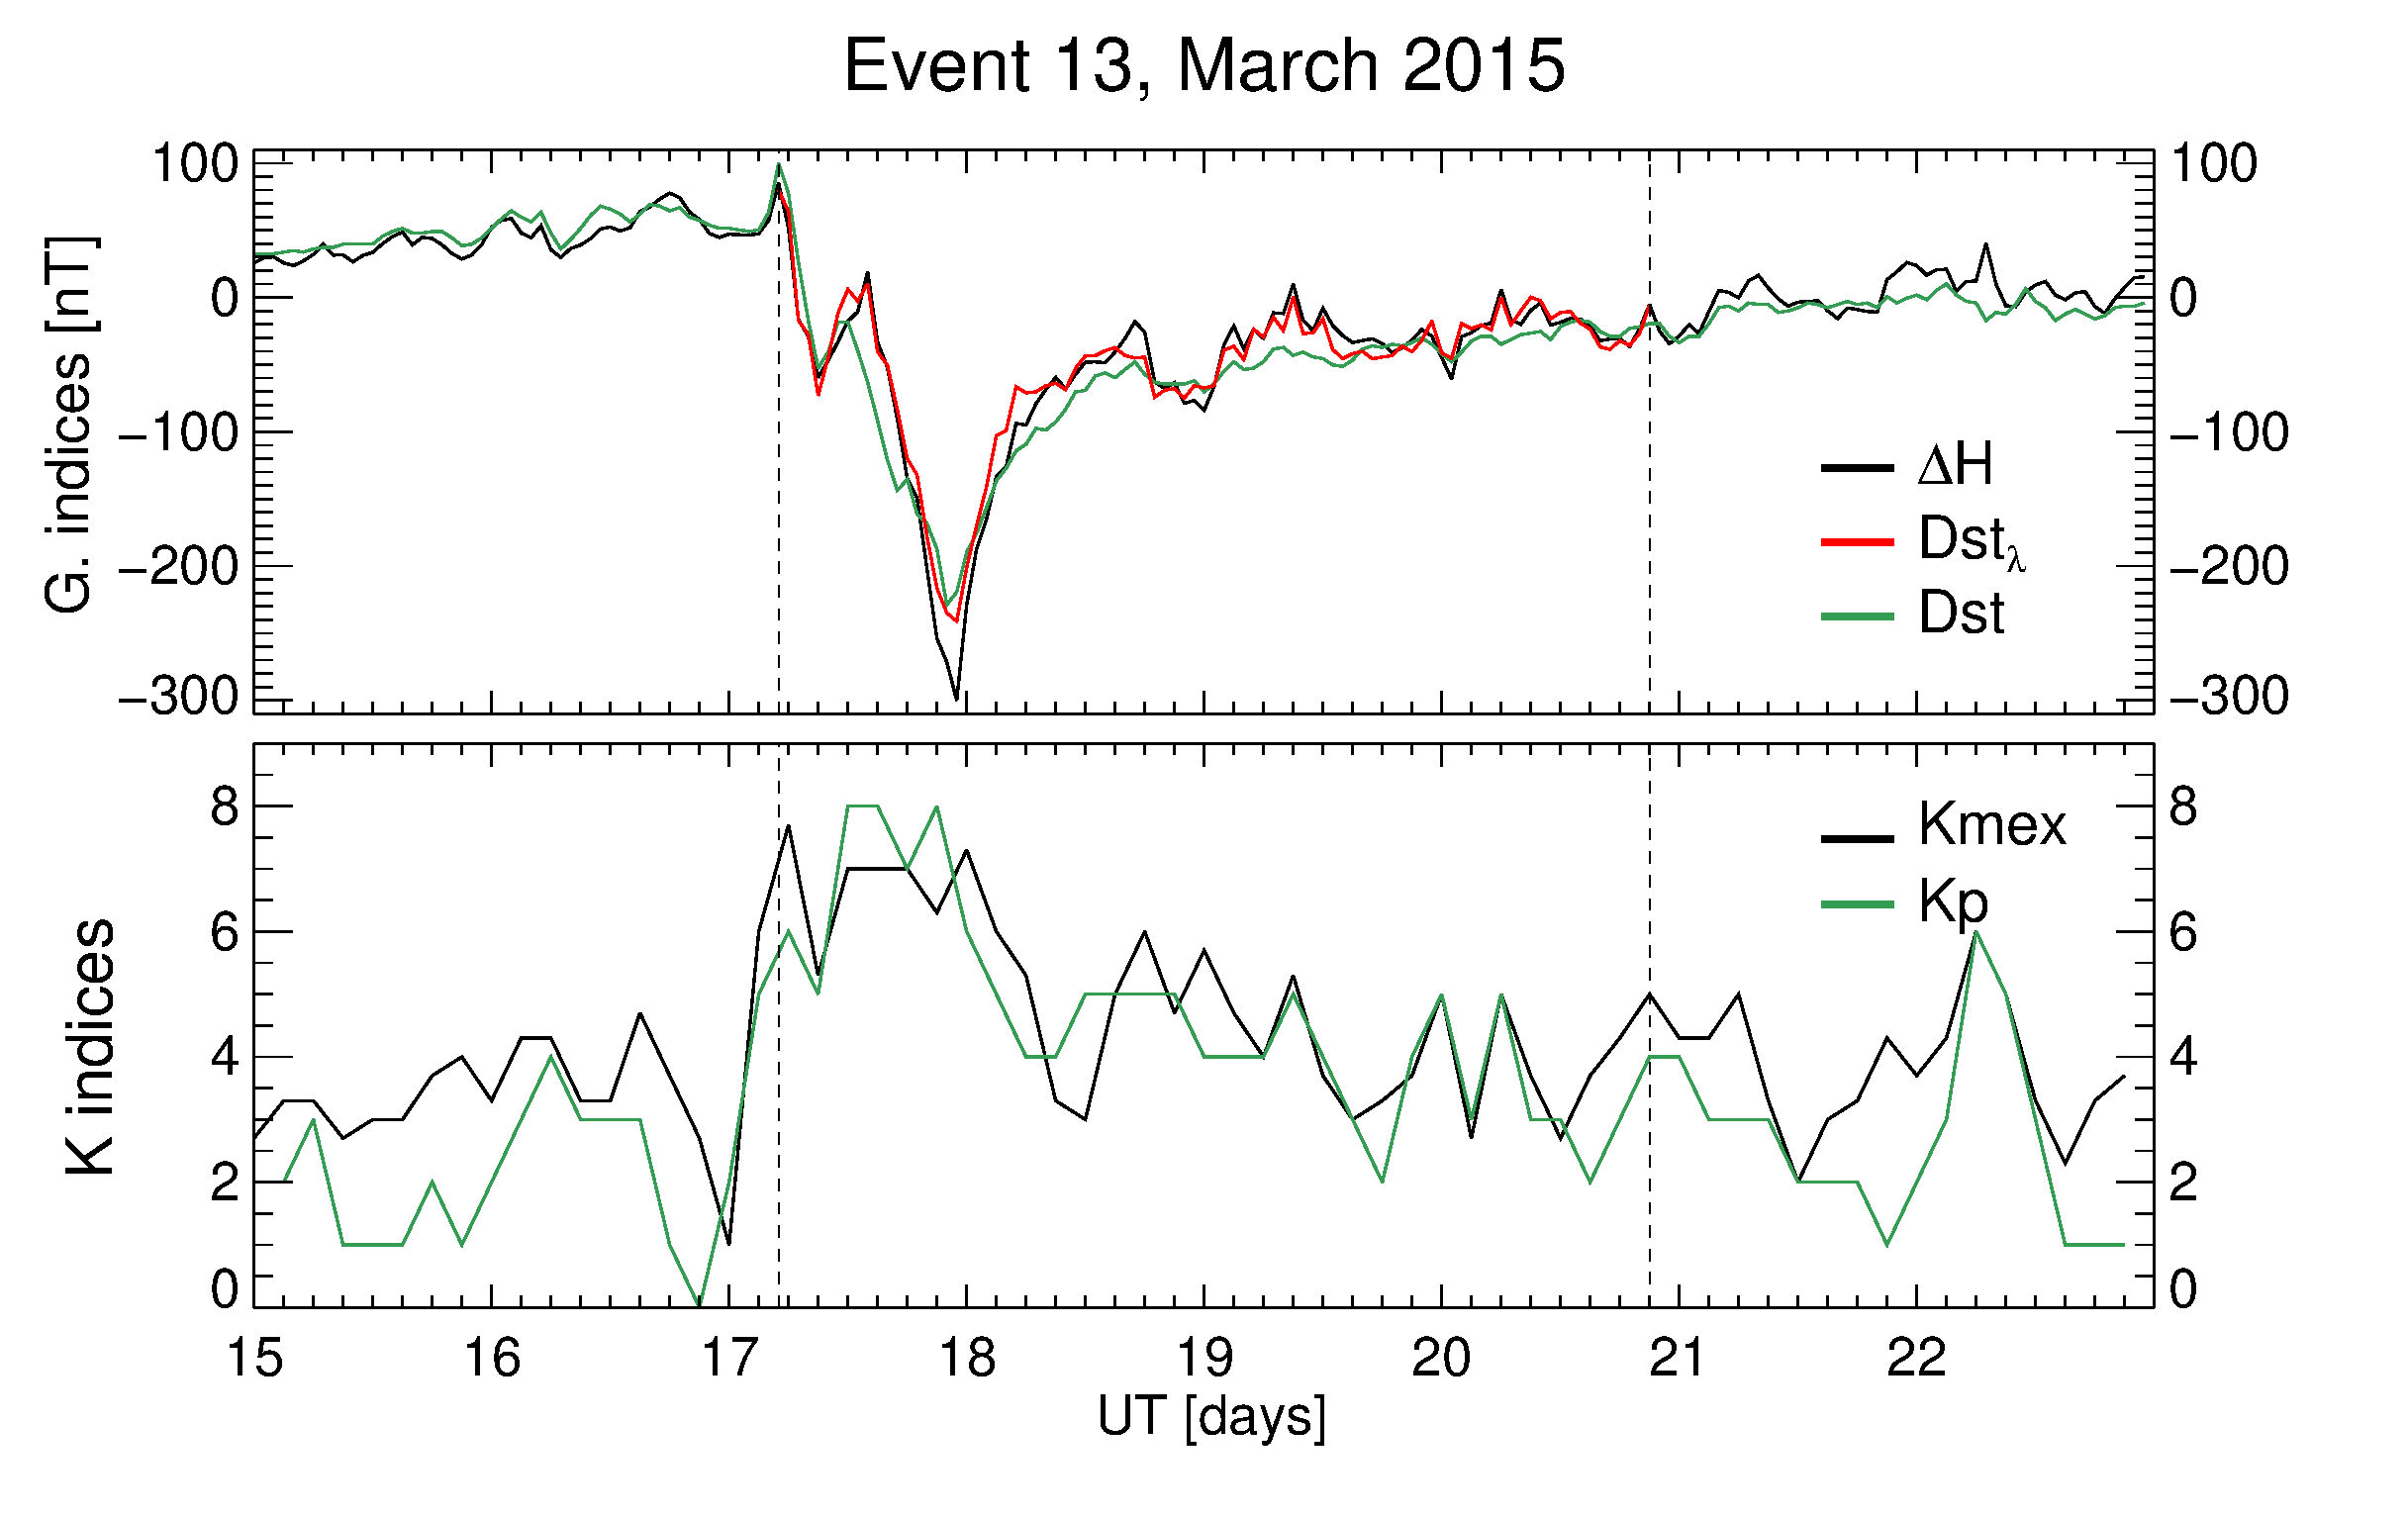
\includegraphics[width=6.0cm]{images/dH_approx/diono_valid_V4_2015-03-15.eps}     
       \centerline{\Large \bf   
      \hspace{0.275\textwidth}  \color{black}{}
       \hspace{0.295\textwidth}  \color{black}{}
         \hfill}   
	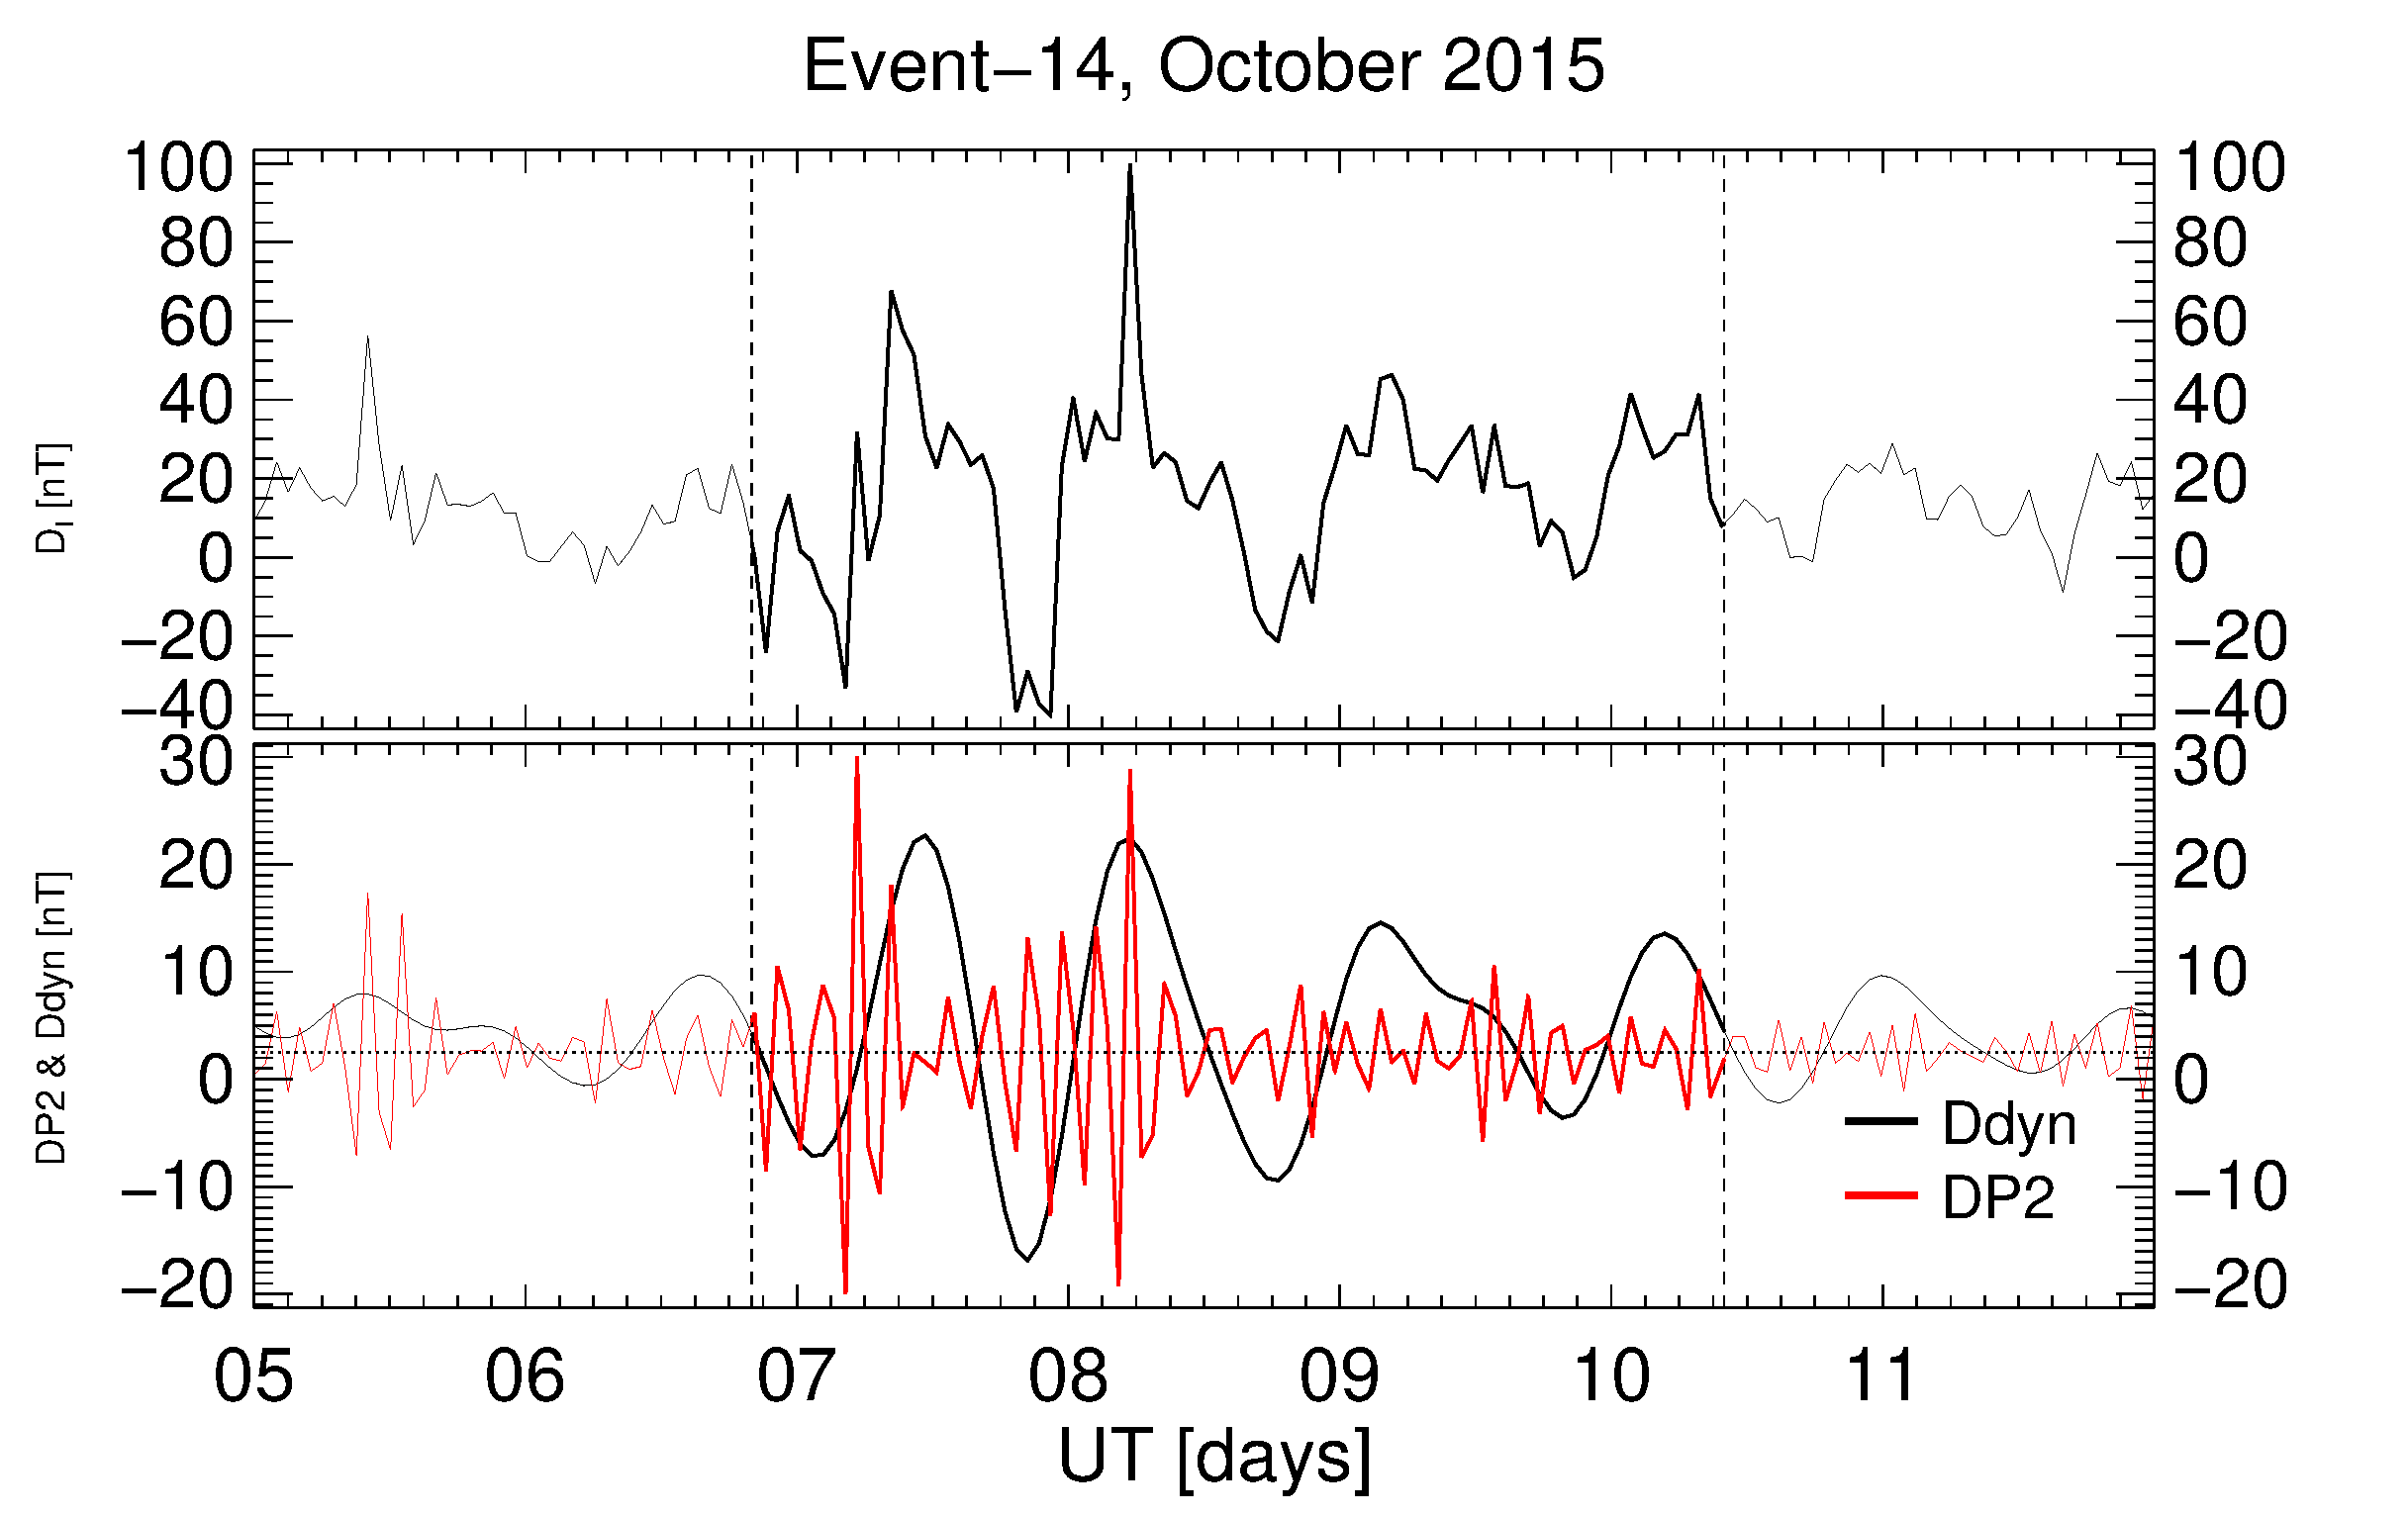
\includegraphics[width=6.0cm]{images/diono/iono_PI_V1_2015-10-05.eps}
    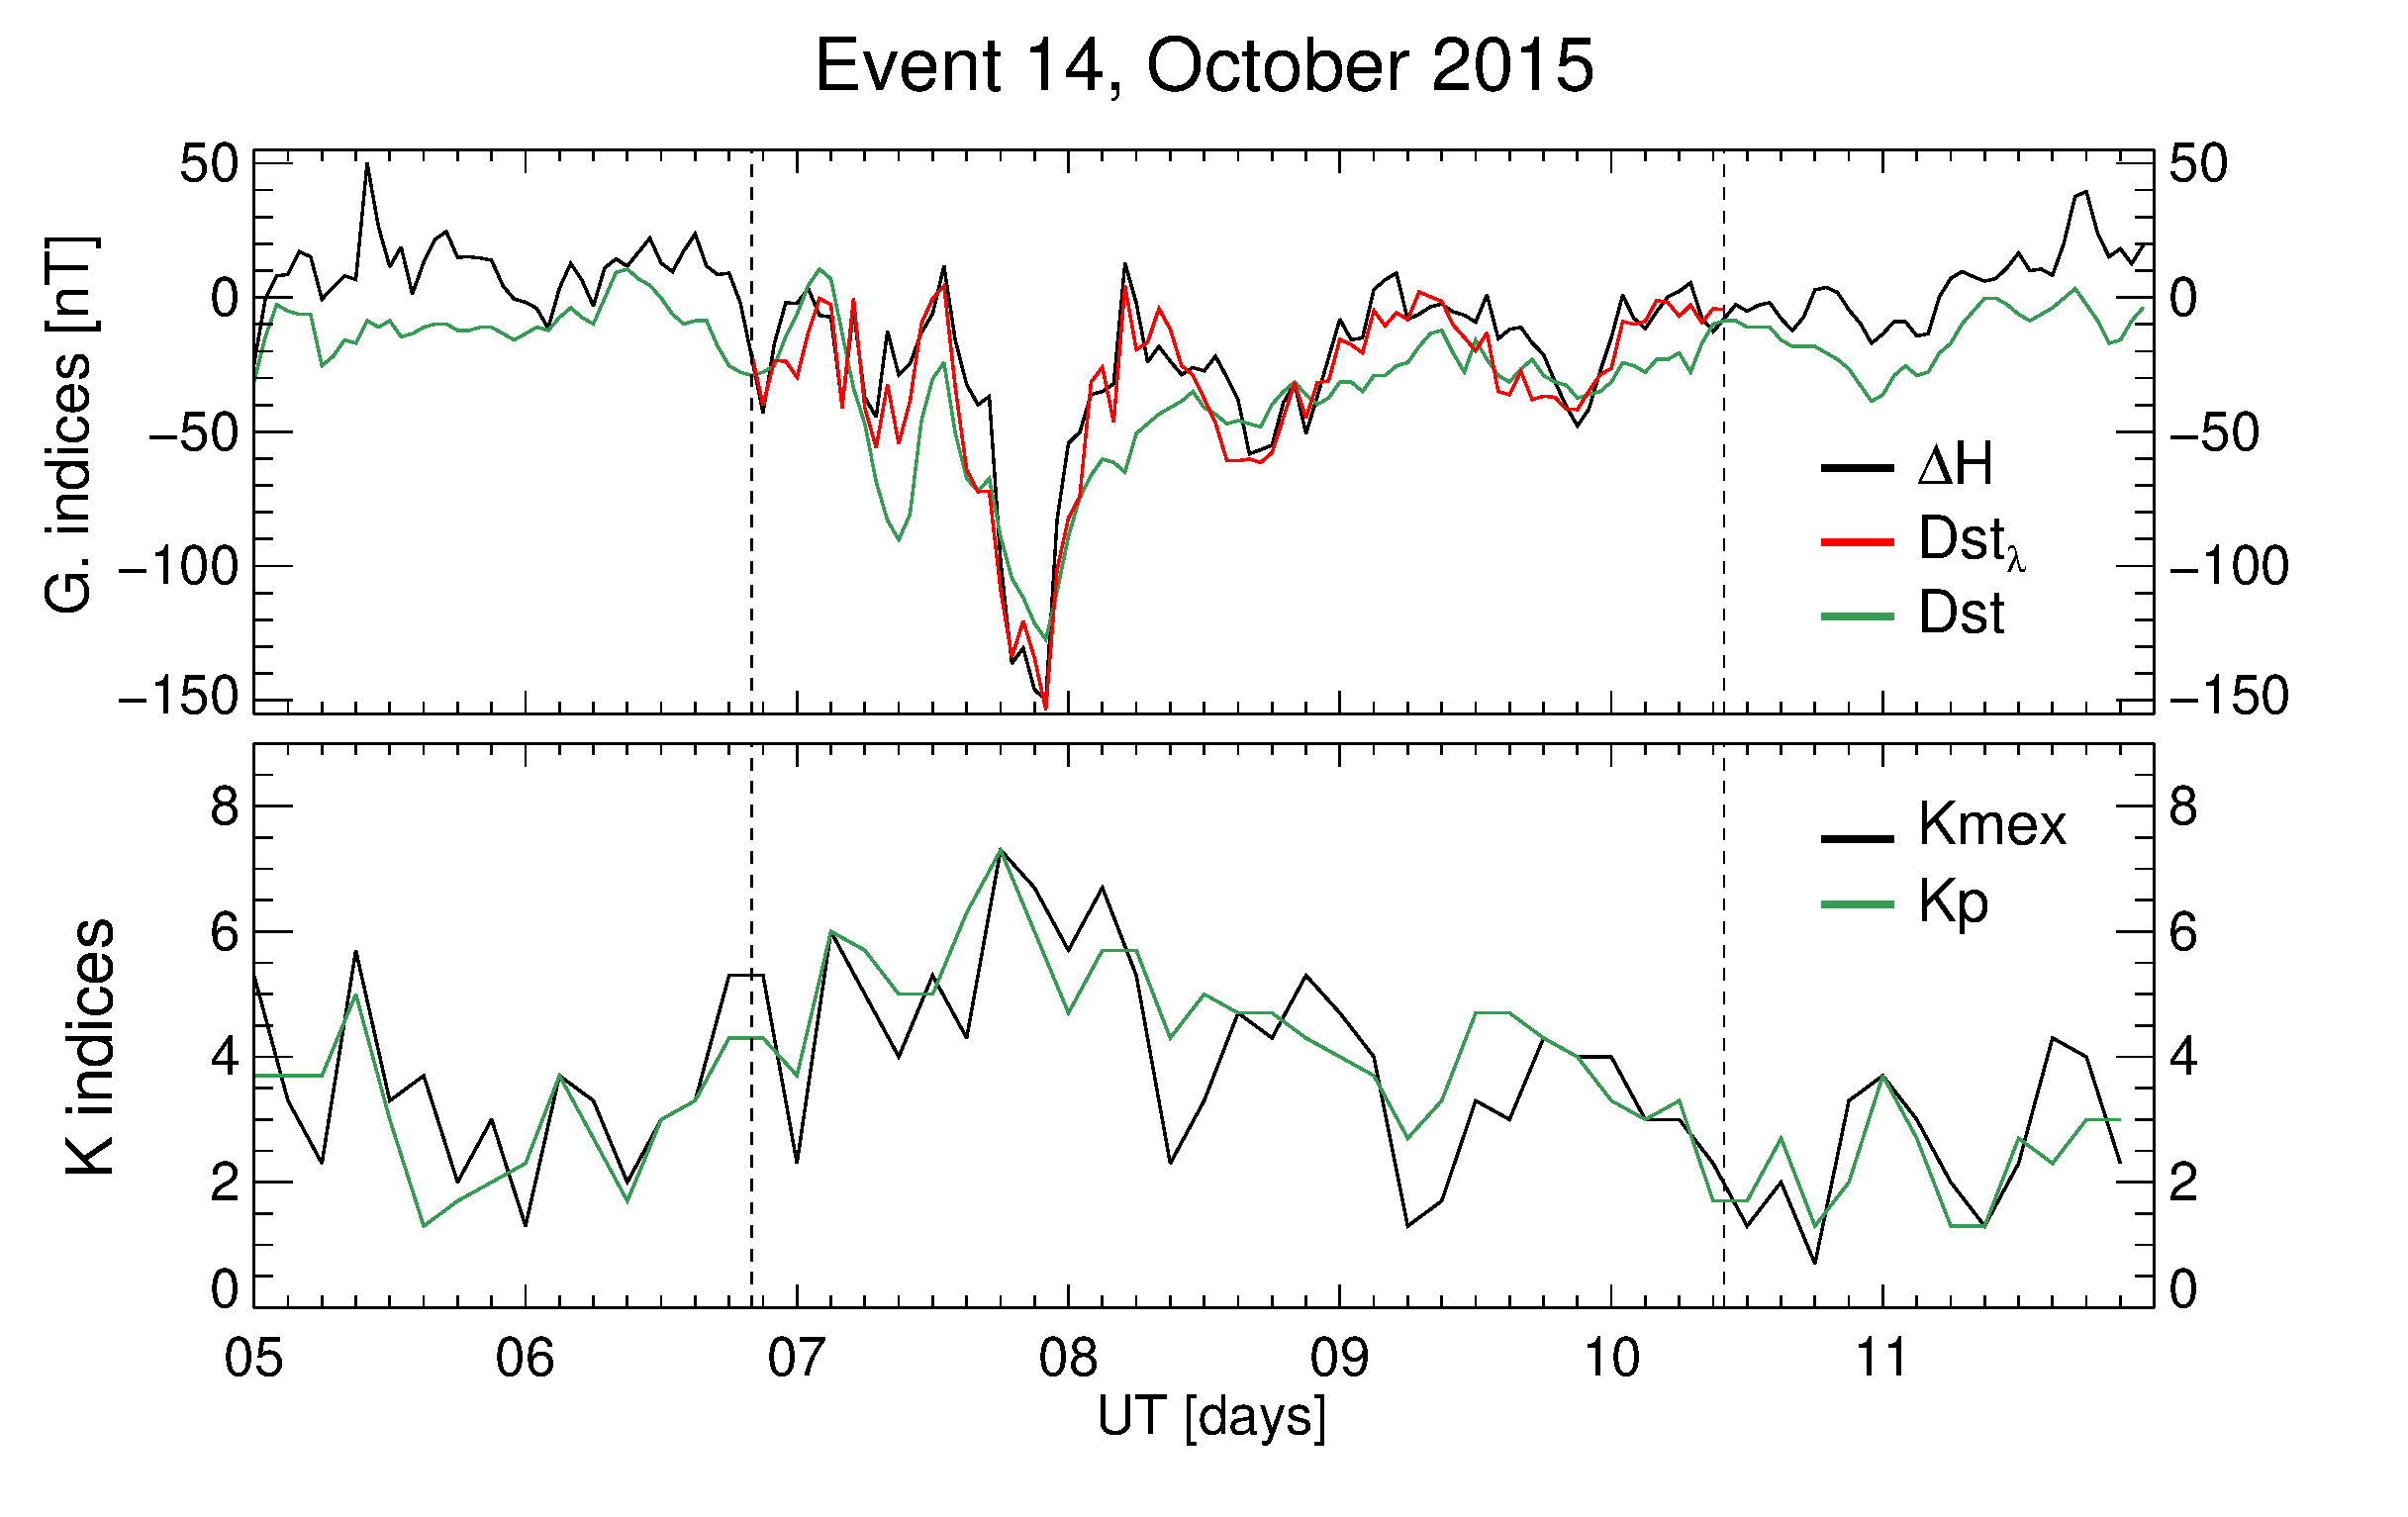
\includegraphics[width=6.0cm]{images/dH_approx/diono_valid_V4_2015-10-05.eps}
    
       \centerline{\Large \bf   
 	\hspace{0.26\textwidth}  \color{black}{}
 	\hspace{0.31\textwidth}  \color{black}{}
 	\hfill}
 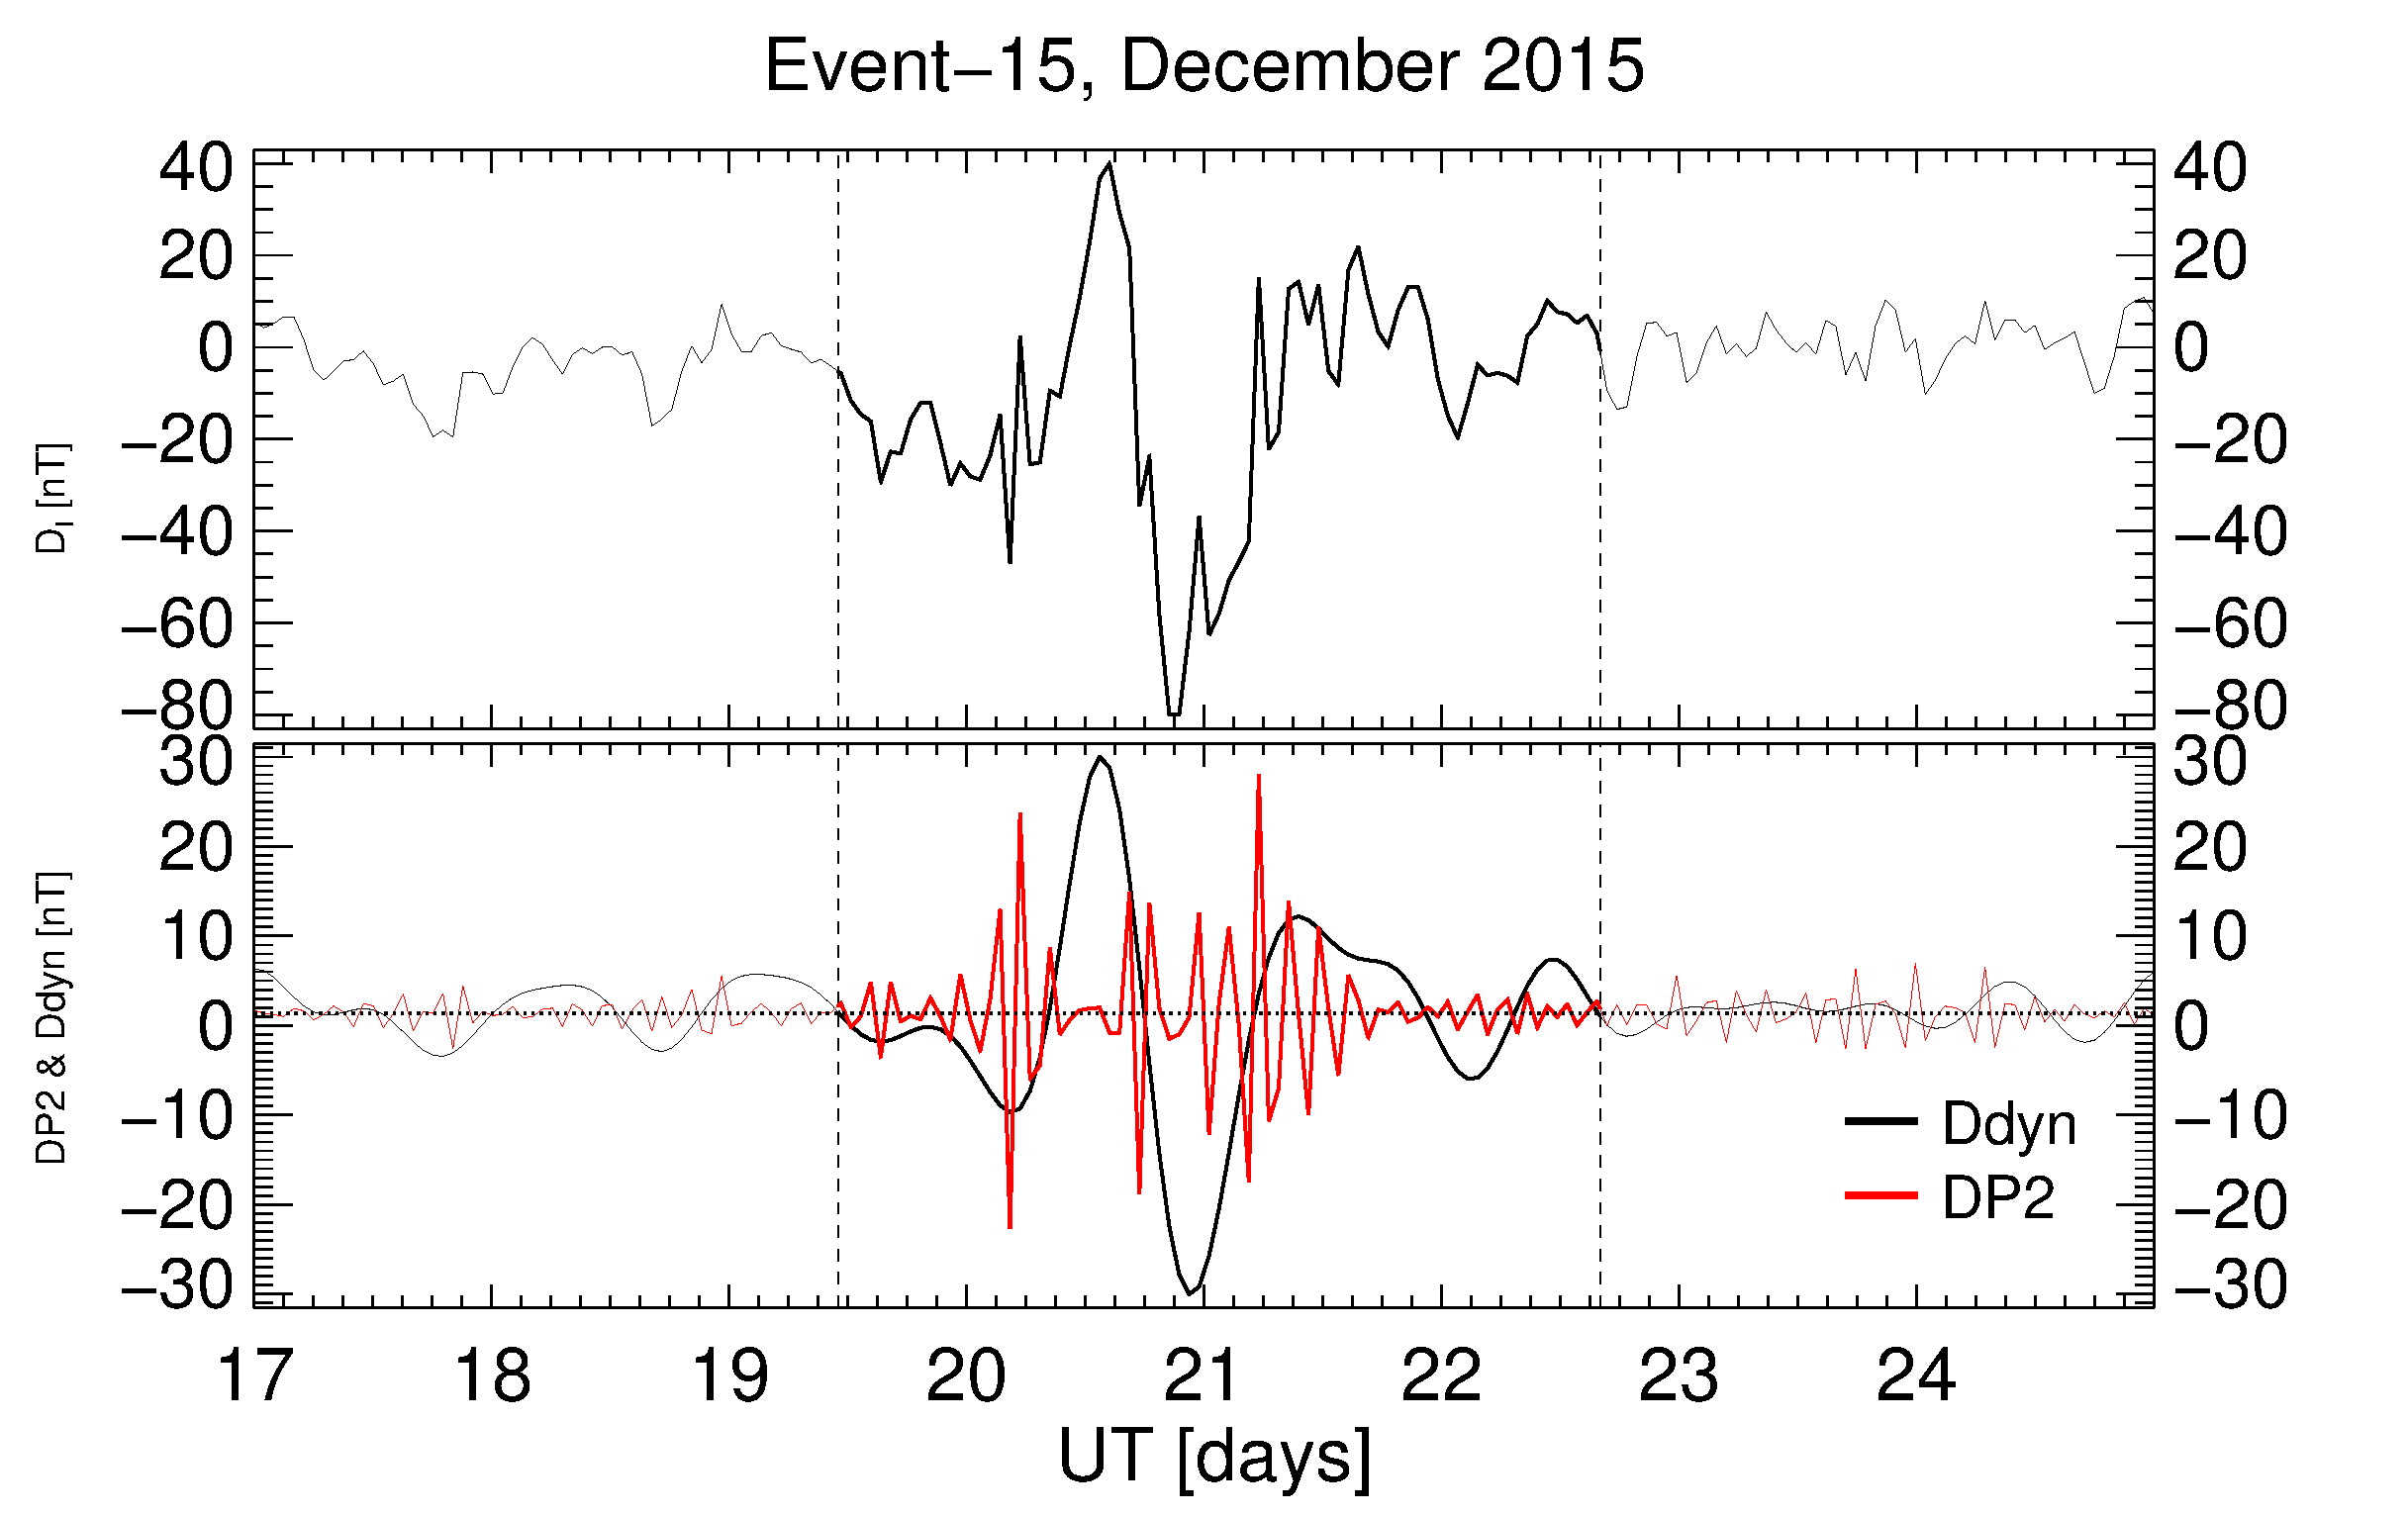
\includegraphics[width=6.0cm]{images/diono/iono_PI_V1_2015-12-17.eps}
 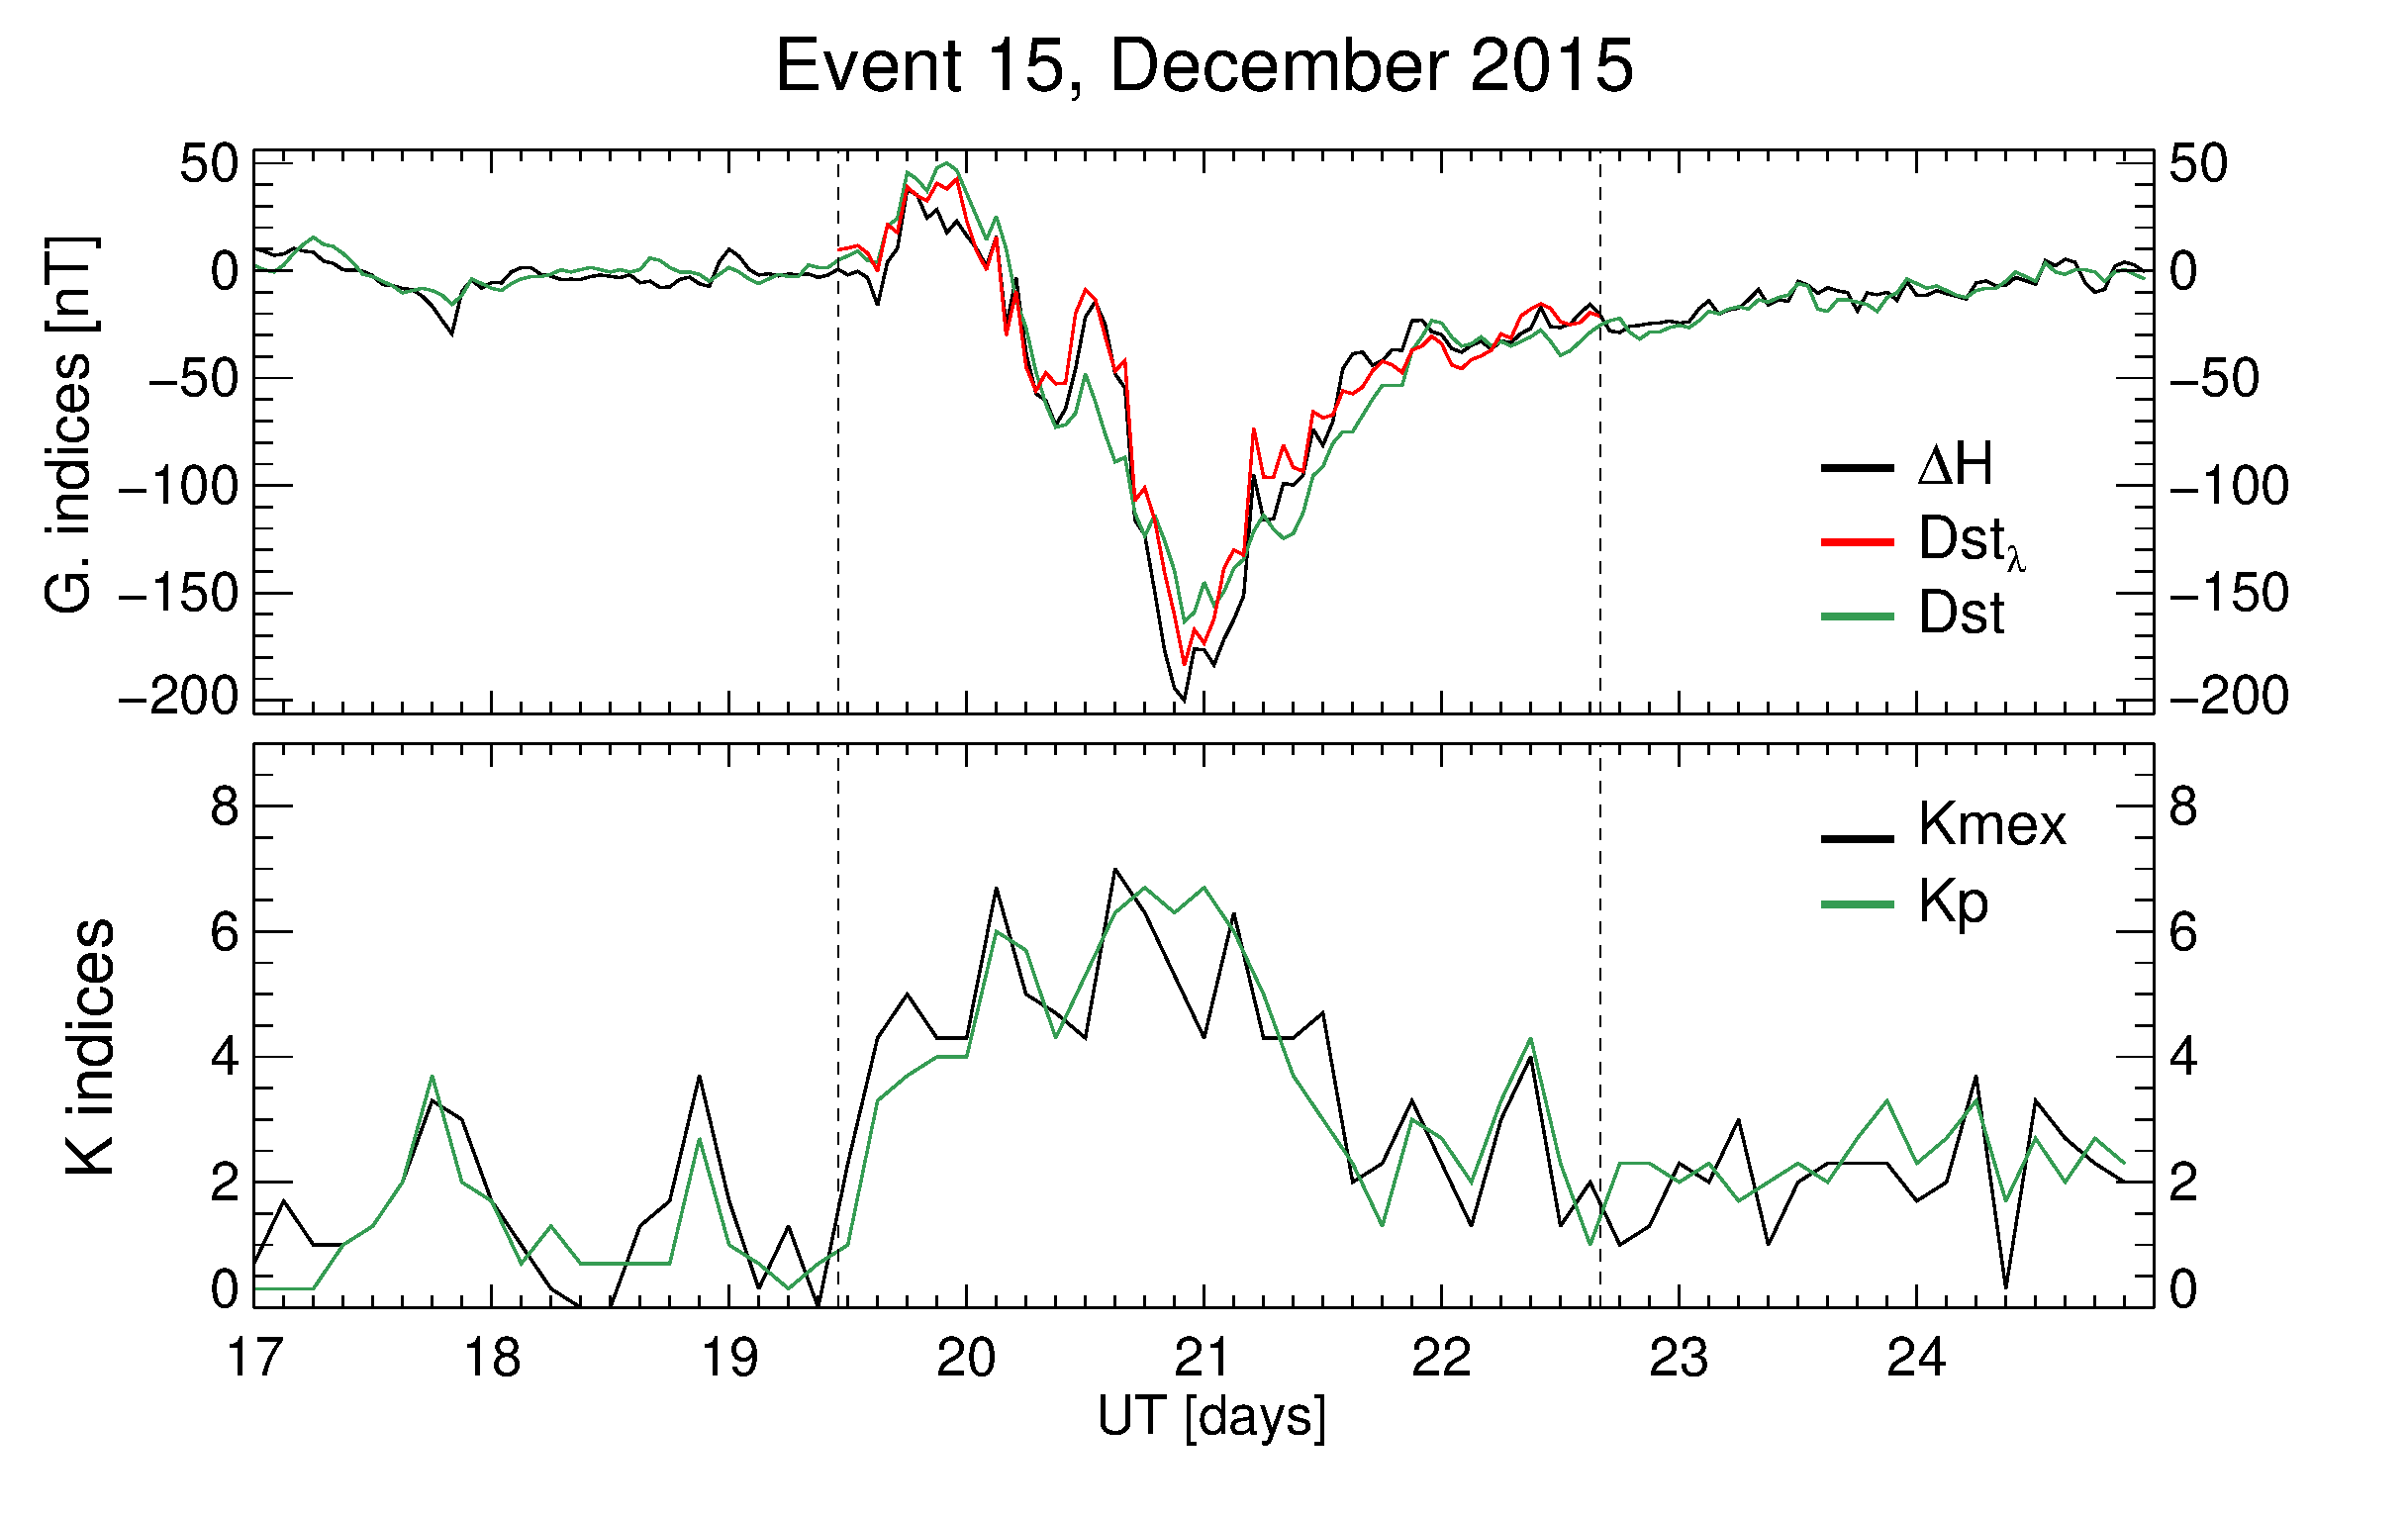
\includegraphics[width=6.0cm]{images/dH_approx/diono_valid_V4_2015-12-17.eps}           
       \caption{On the right side, top panels illustrate the contribution of Ionospheric Magnetic Disturbances, while bottom panels depict the isolated geomagnetic contributions of $Ddyn$ and $DP2$. The vertical dashed lines highlight the geomagnetic storm time period during which such calculations are valid. On the left side, green lines represent planetary indices, while black lines denote local indices. Additionally, red lines represent the approximation of $\Delta H$ at top, while bottom showcases the comparison of local $K$ (black line) and planetary $K$ (green line).
       }
    \label{fig:iono_valid2}
\end{figure*}


\begin{figure*}[h!]
    \centering
    \centerline{\Large \bf   
      %\hspace{0.18\textwidth}  \color{black}{\Large{Res}}
       %\hspace{0.28\textwidth}
      %\color{black}{\Large{Res+TC}}
         \hfill}
          \centerline{\Large \bf   
      \hspace{0.26\textwidth}  \color{black}{}
       \hspace{0.31\textwidth}  \color{black}{}
         \hfill}
    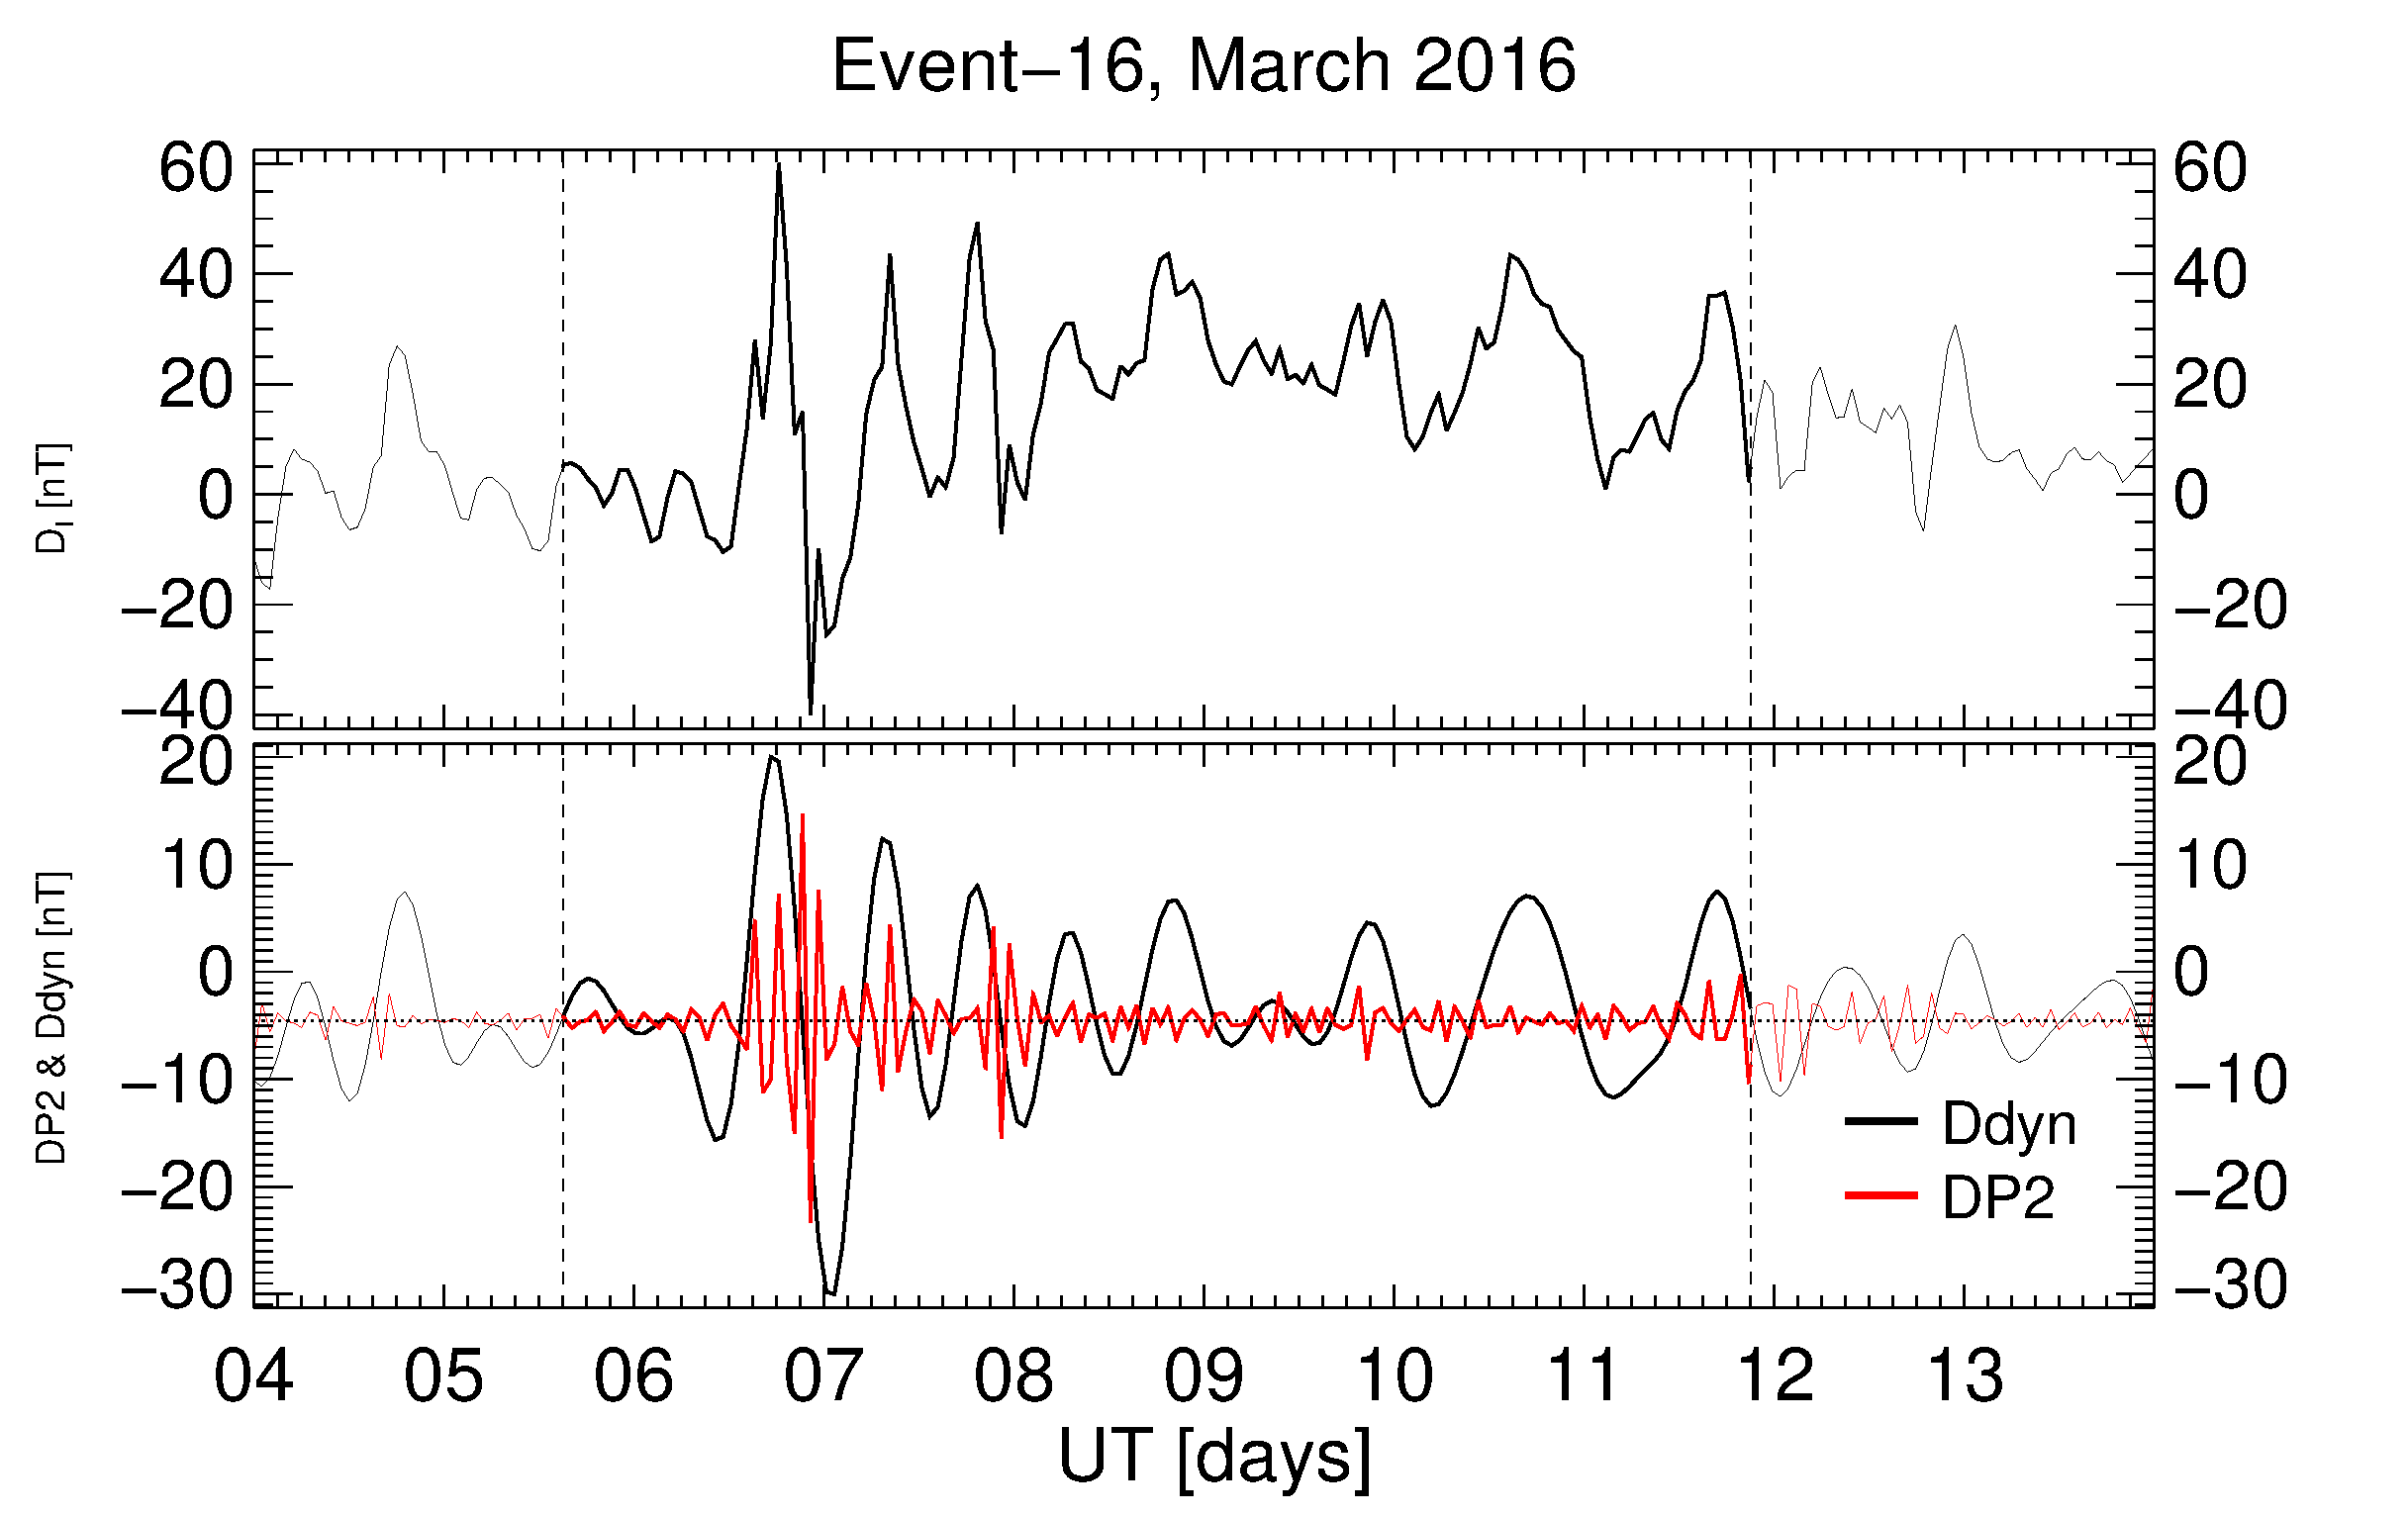
\includegraphics[width=6.0cm]{images/diono/iono_PI_V1_2016-03-04.eps}   
	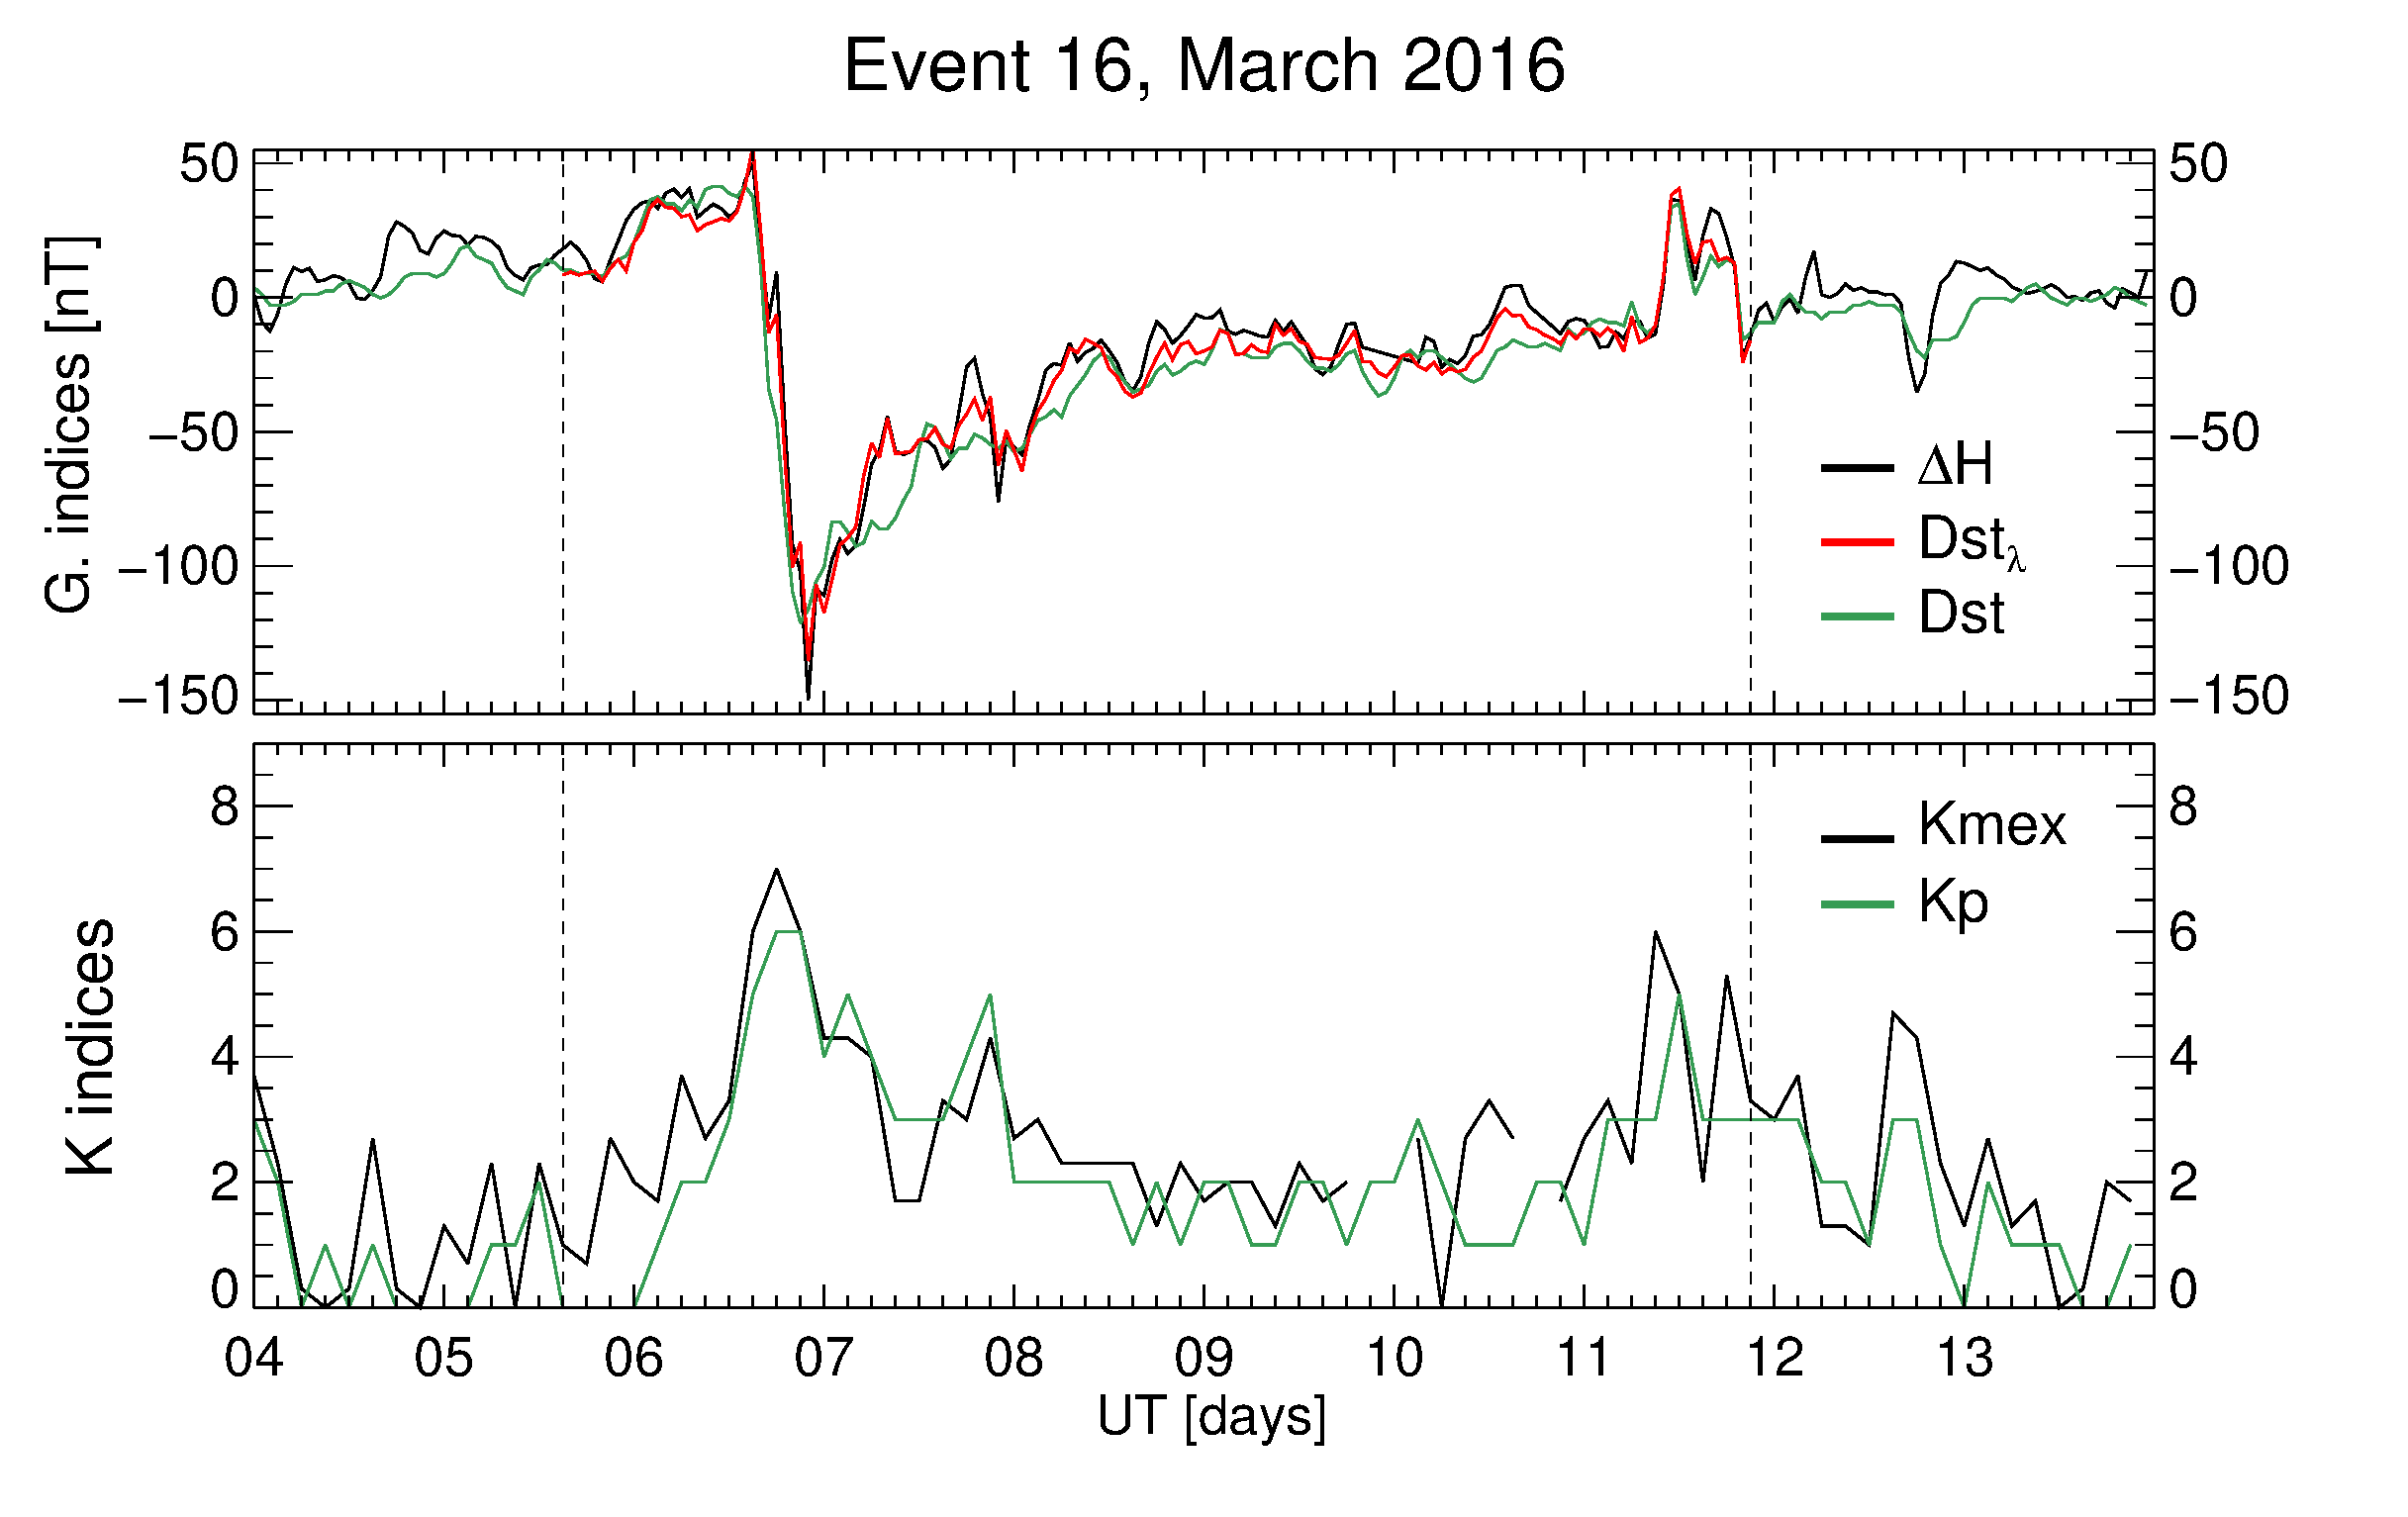
\includegraphics[width=6.0cm]{images/dH_approx/diono_valid_V4_2016-03-04.eps} 	 
     \centerline{\Large \bf   
      \hspace{0.275\textwidth}  \color{black}{}
       \hspace{0.295\textwidth}  \color{black}{}
         \hfill}
    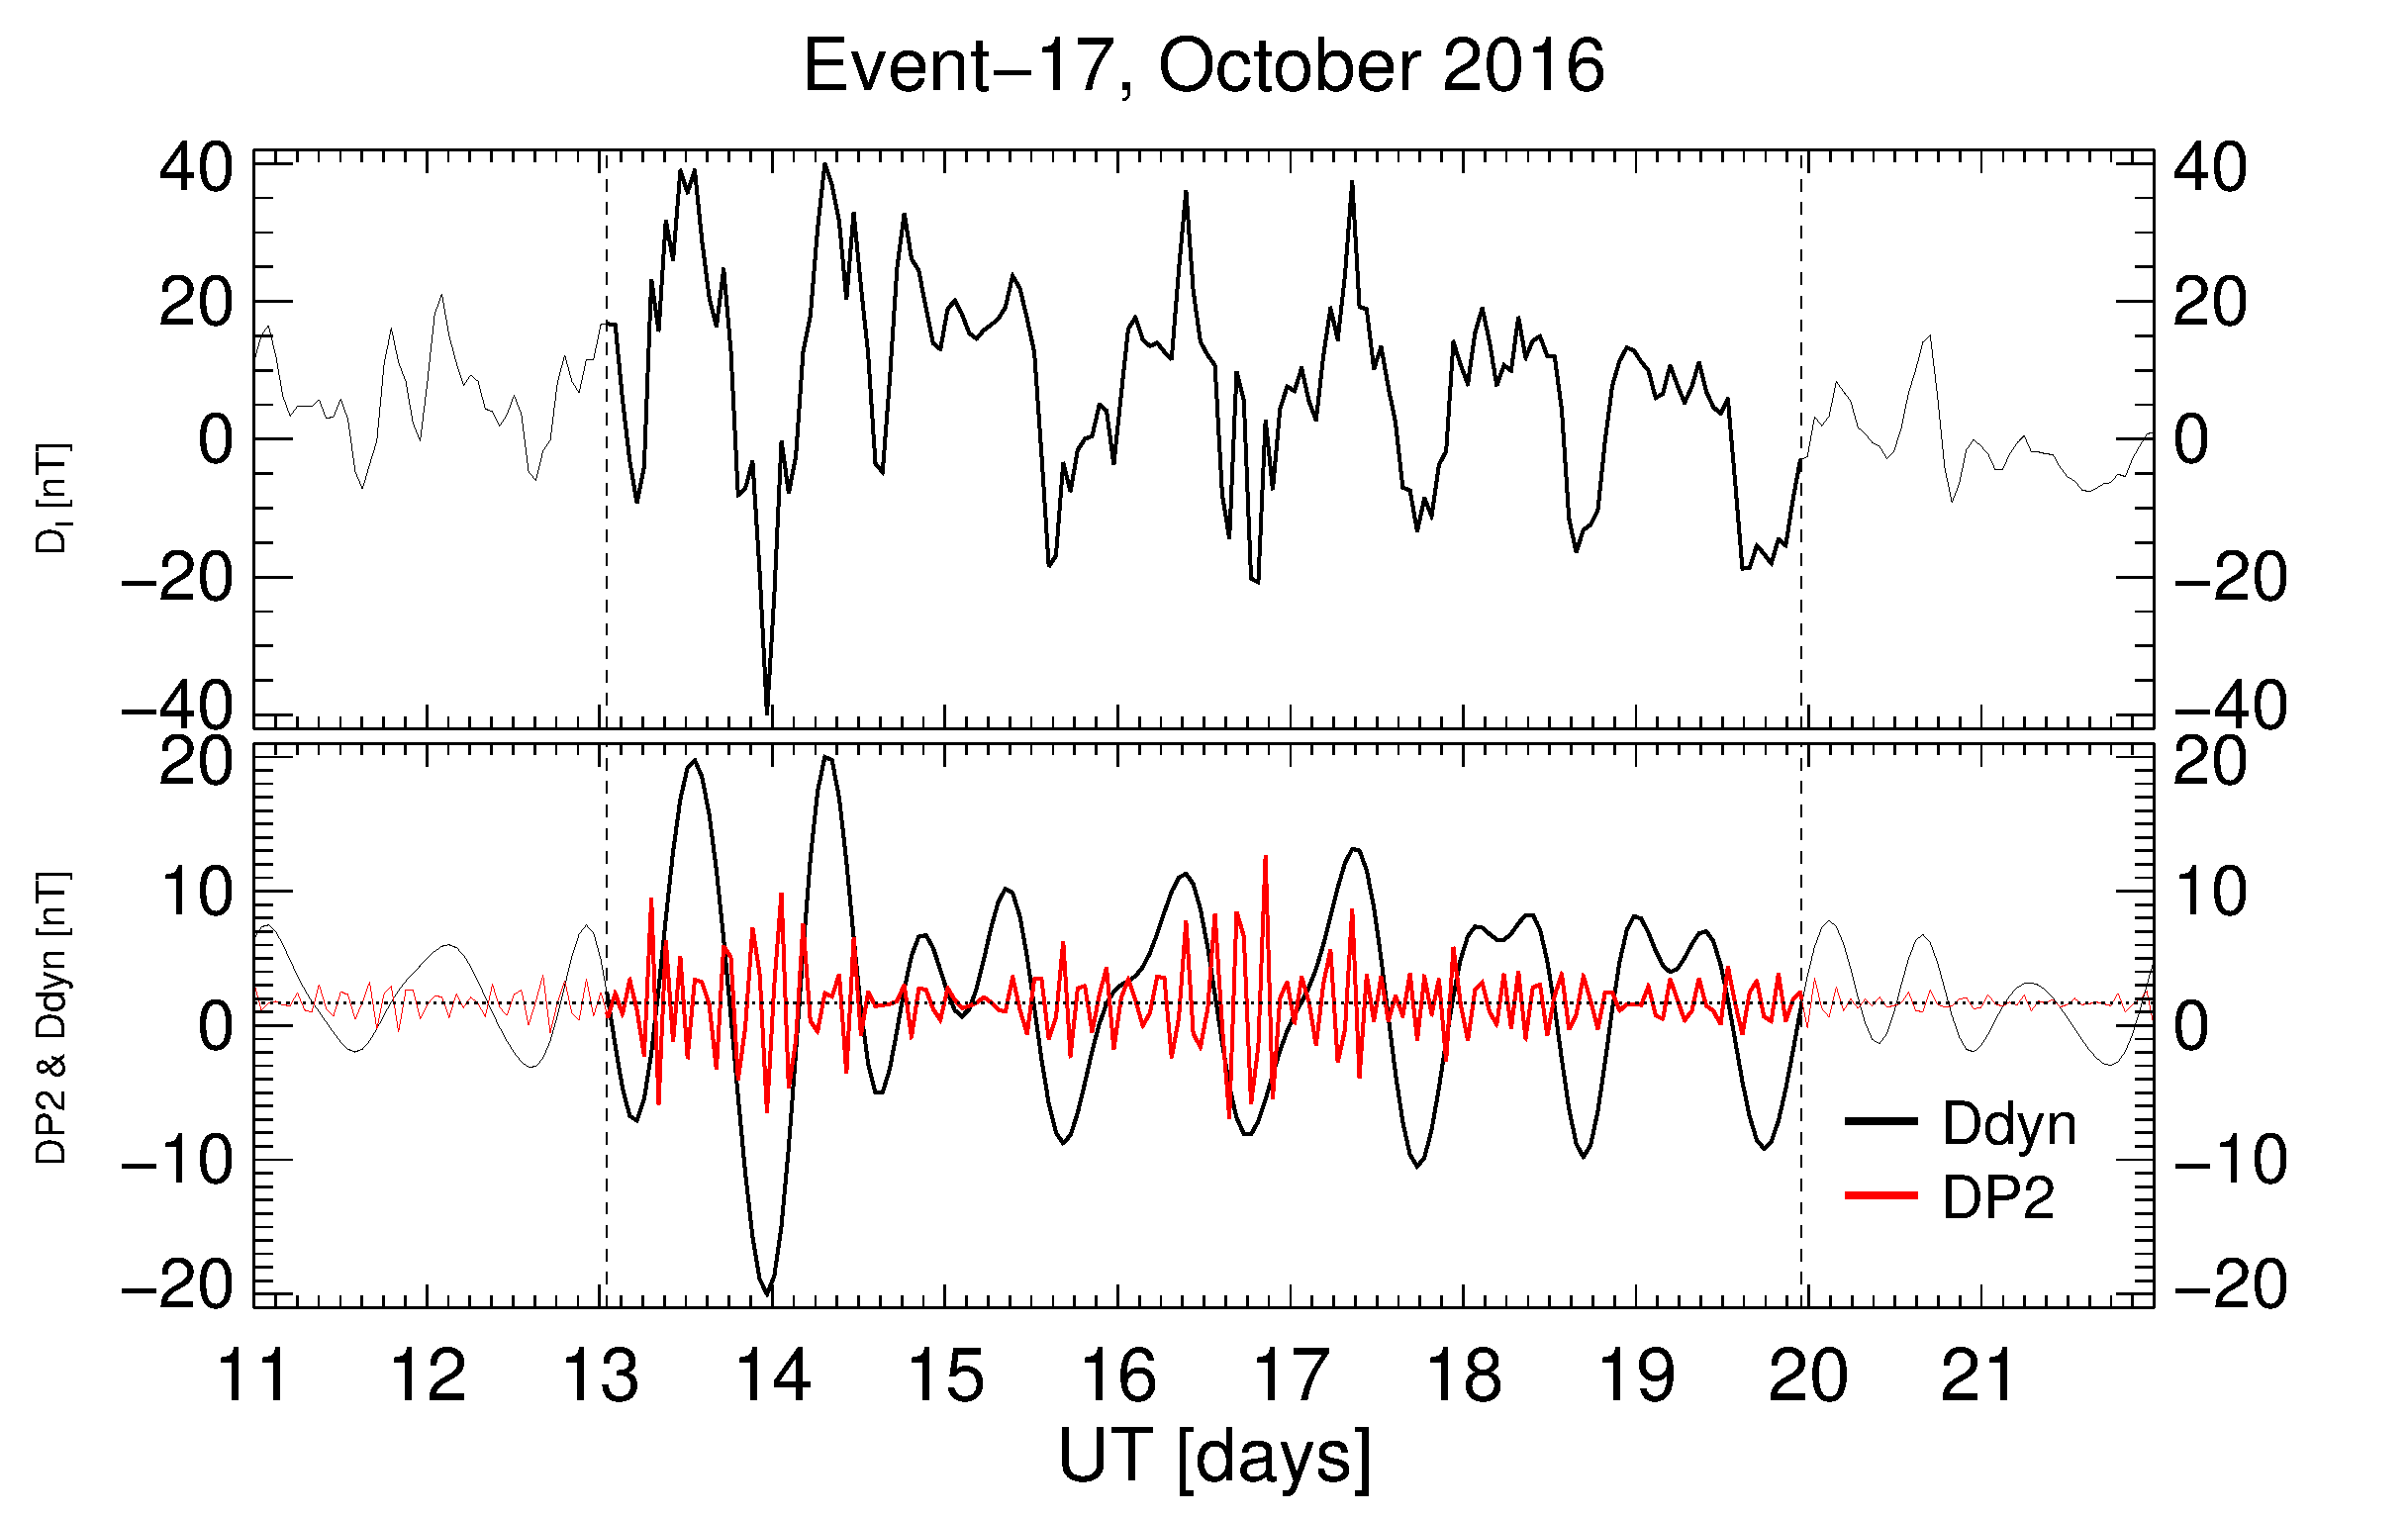
\includegraphics[width=6.0cm]{images/diono/iono_PI_V1_2016-10-11.eps}  
	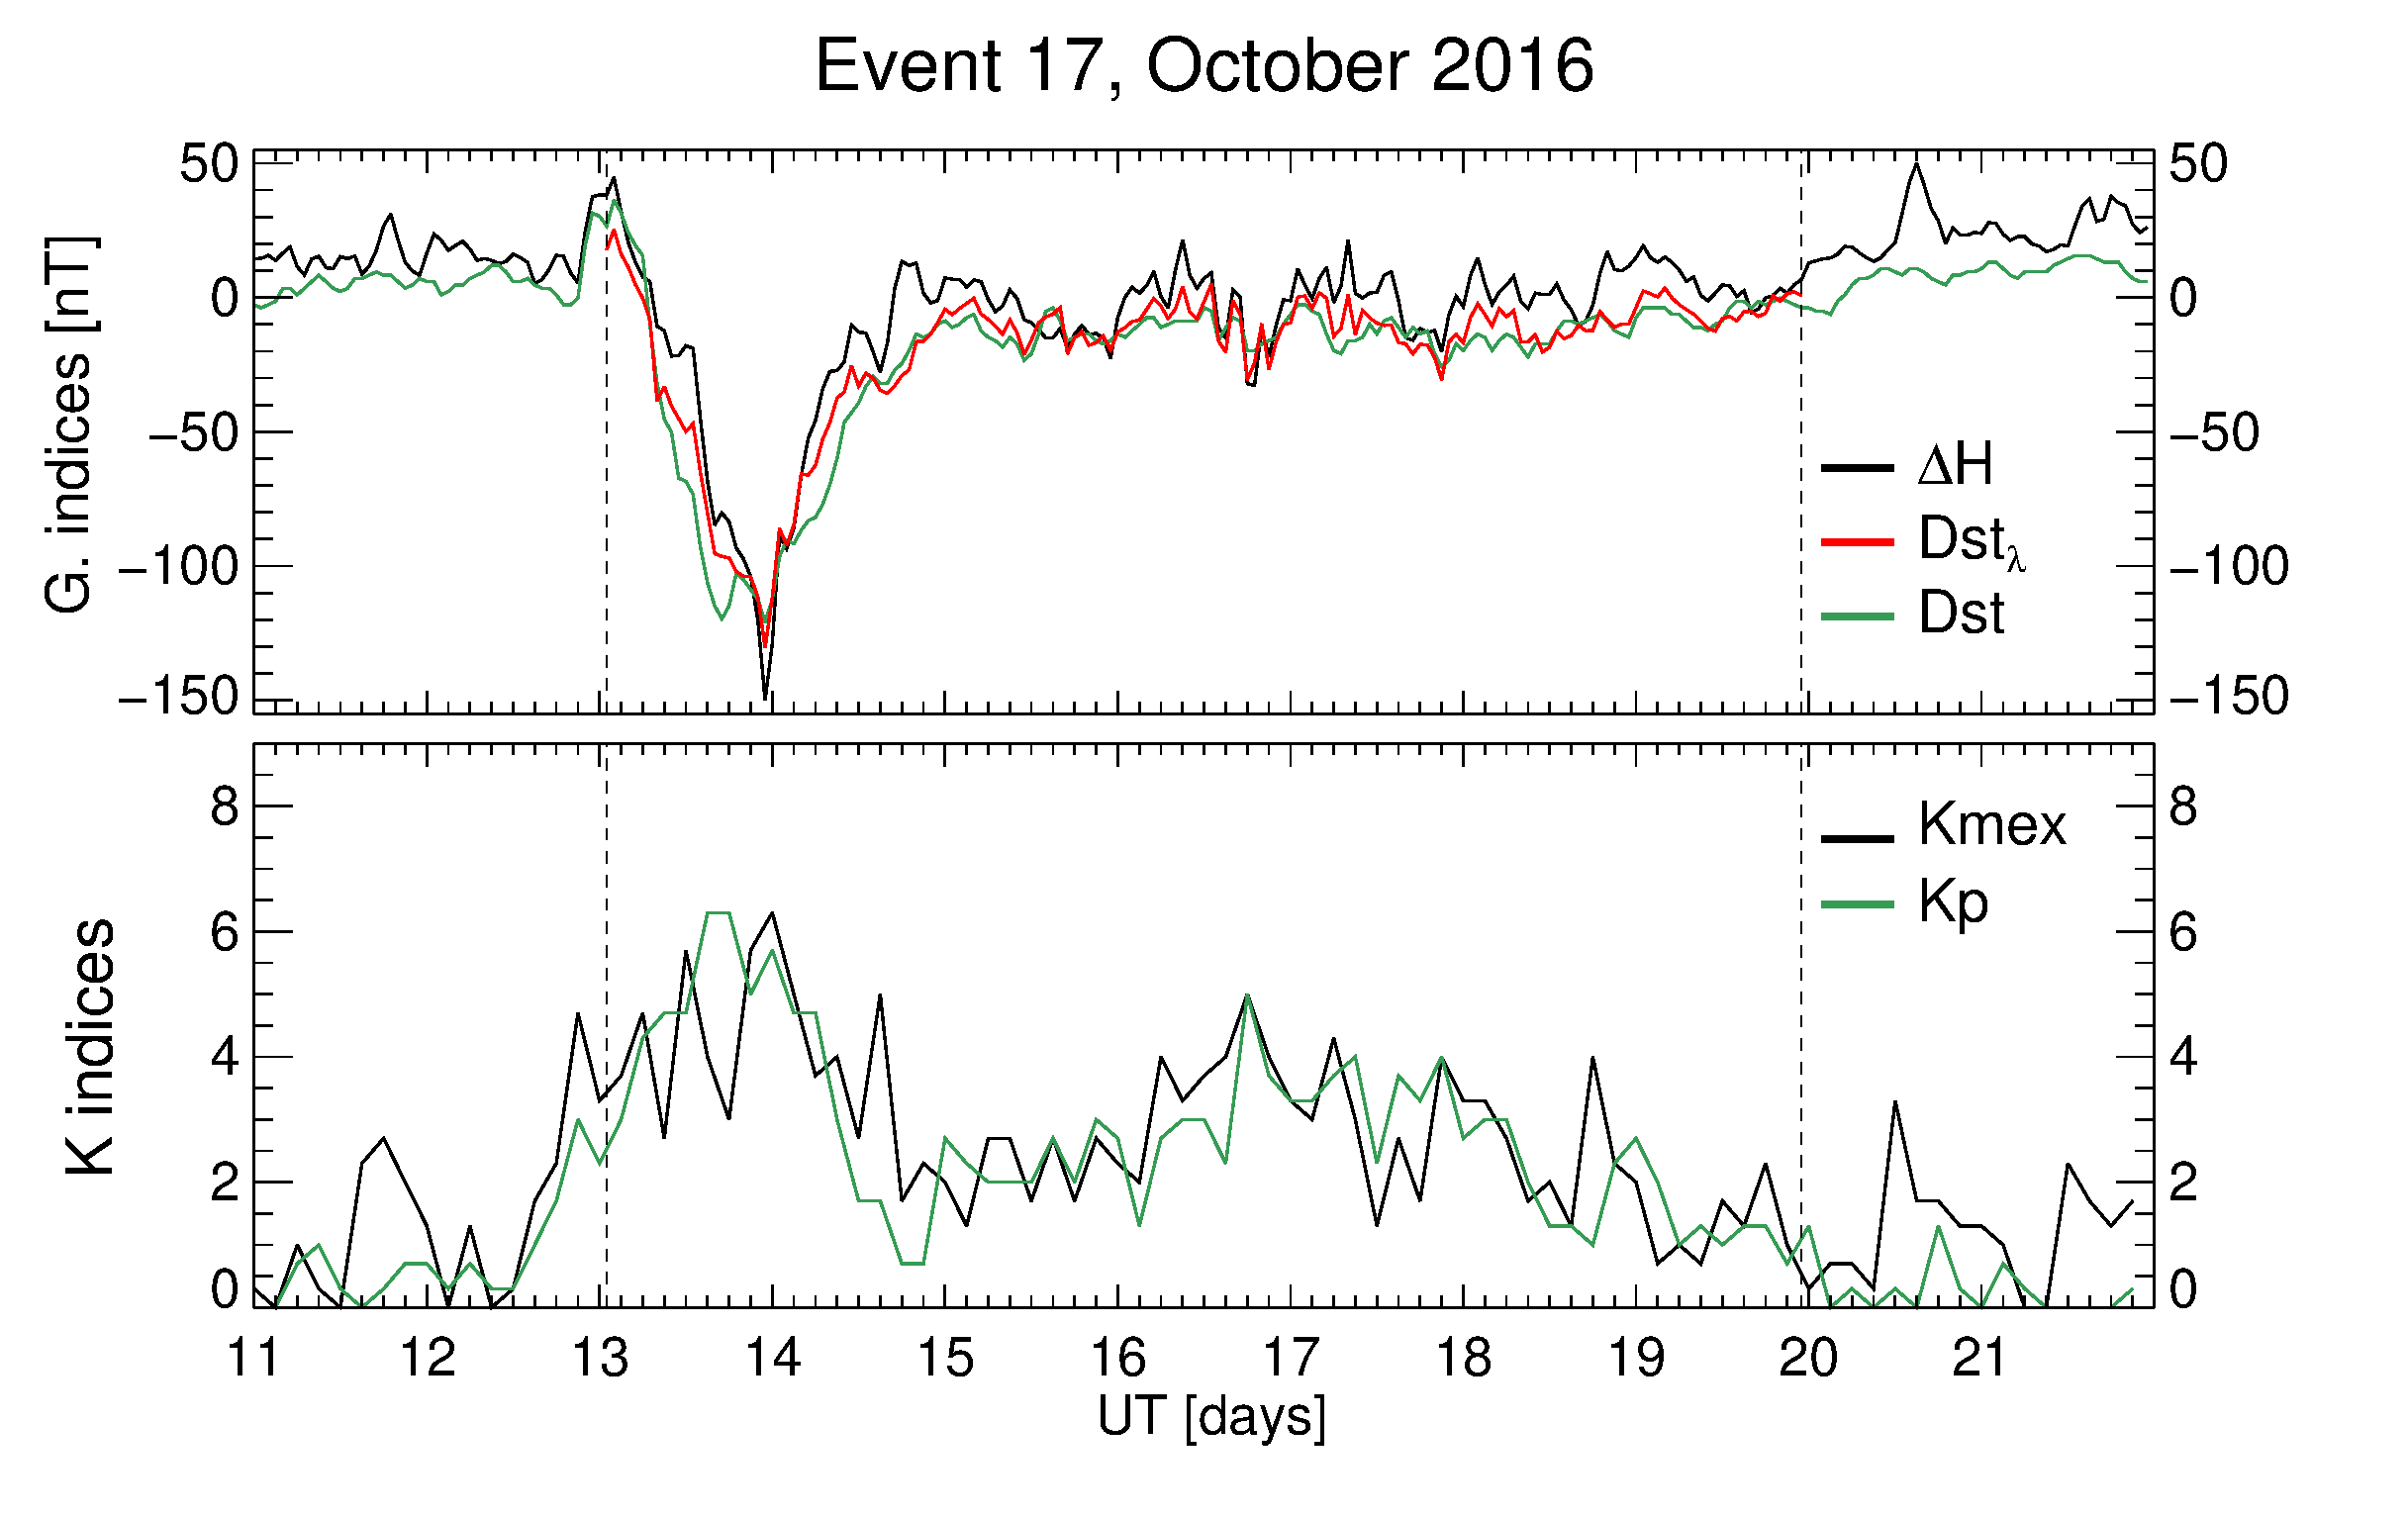
\includegraphics[width=6.0cm]{images/dH_approx/diono_valid_V4_2016-10-11.eps}
     \centerline{\Large \bf   
      \hspace{0.275\textwidth}  \color{black}{}
       \hspace{0.295\textwidth}  \color{black}{}
         \hfill}
    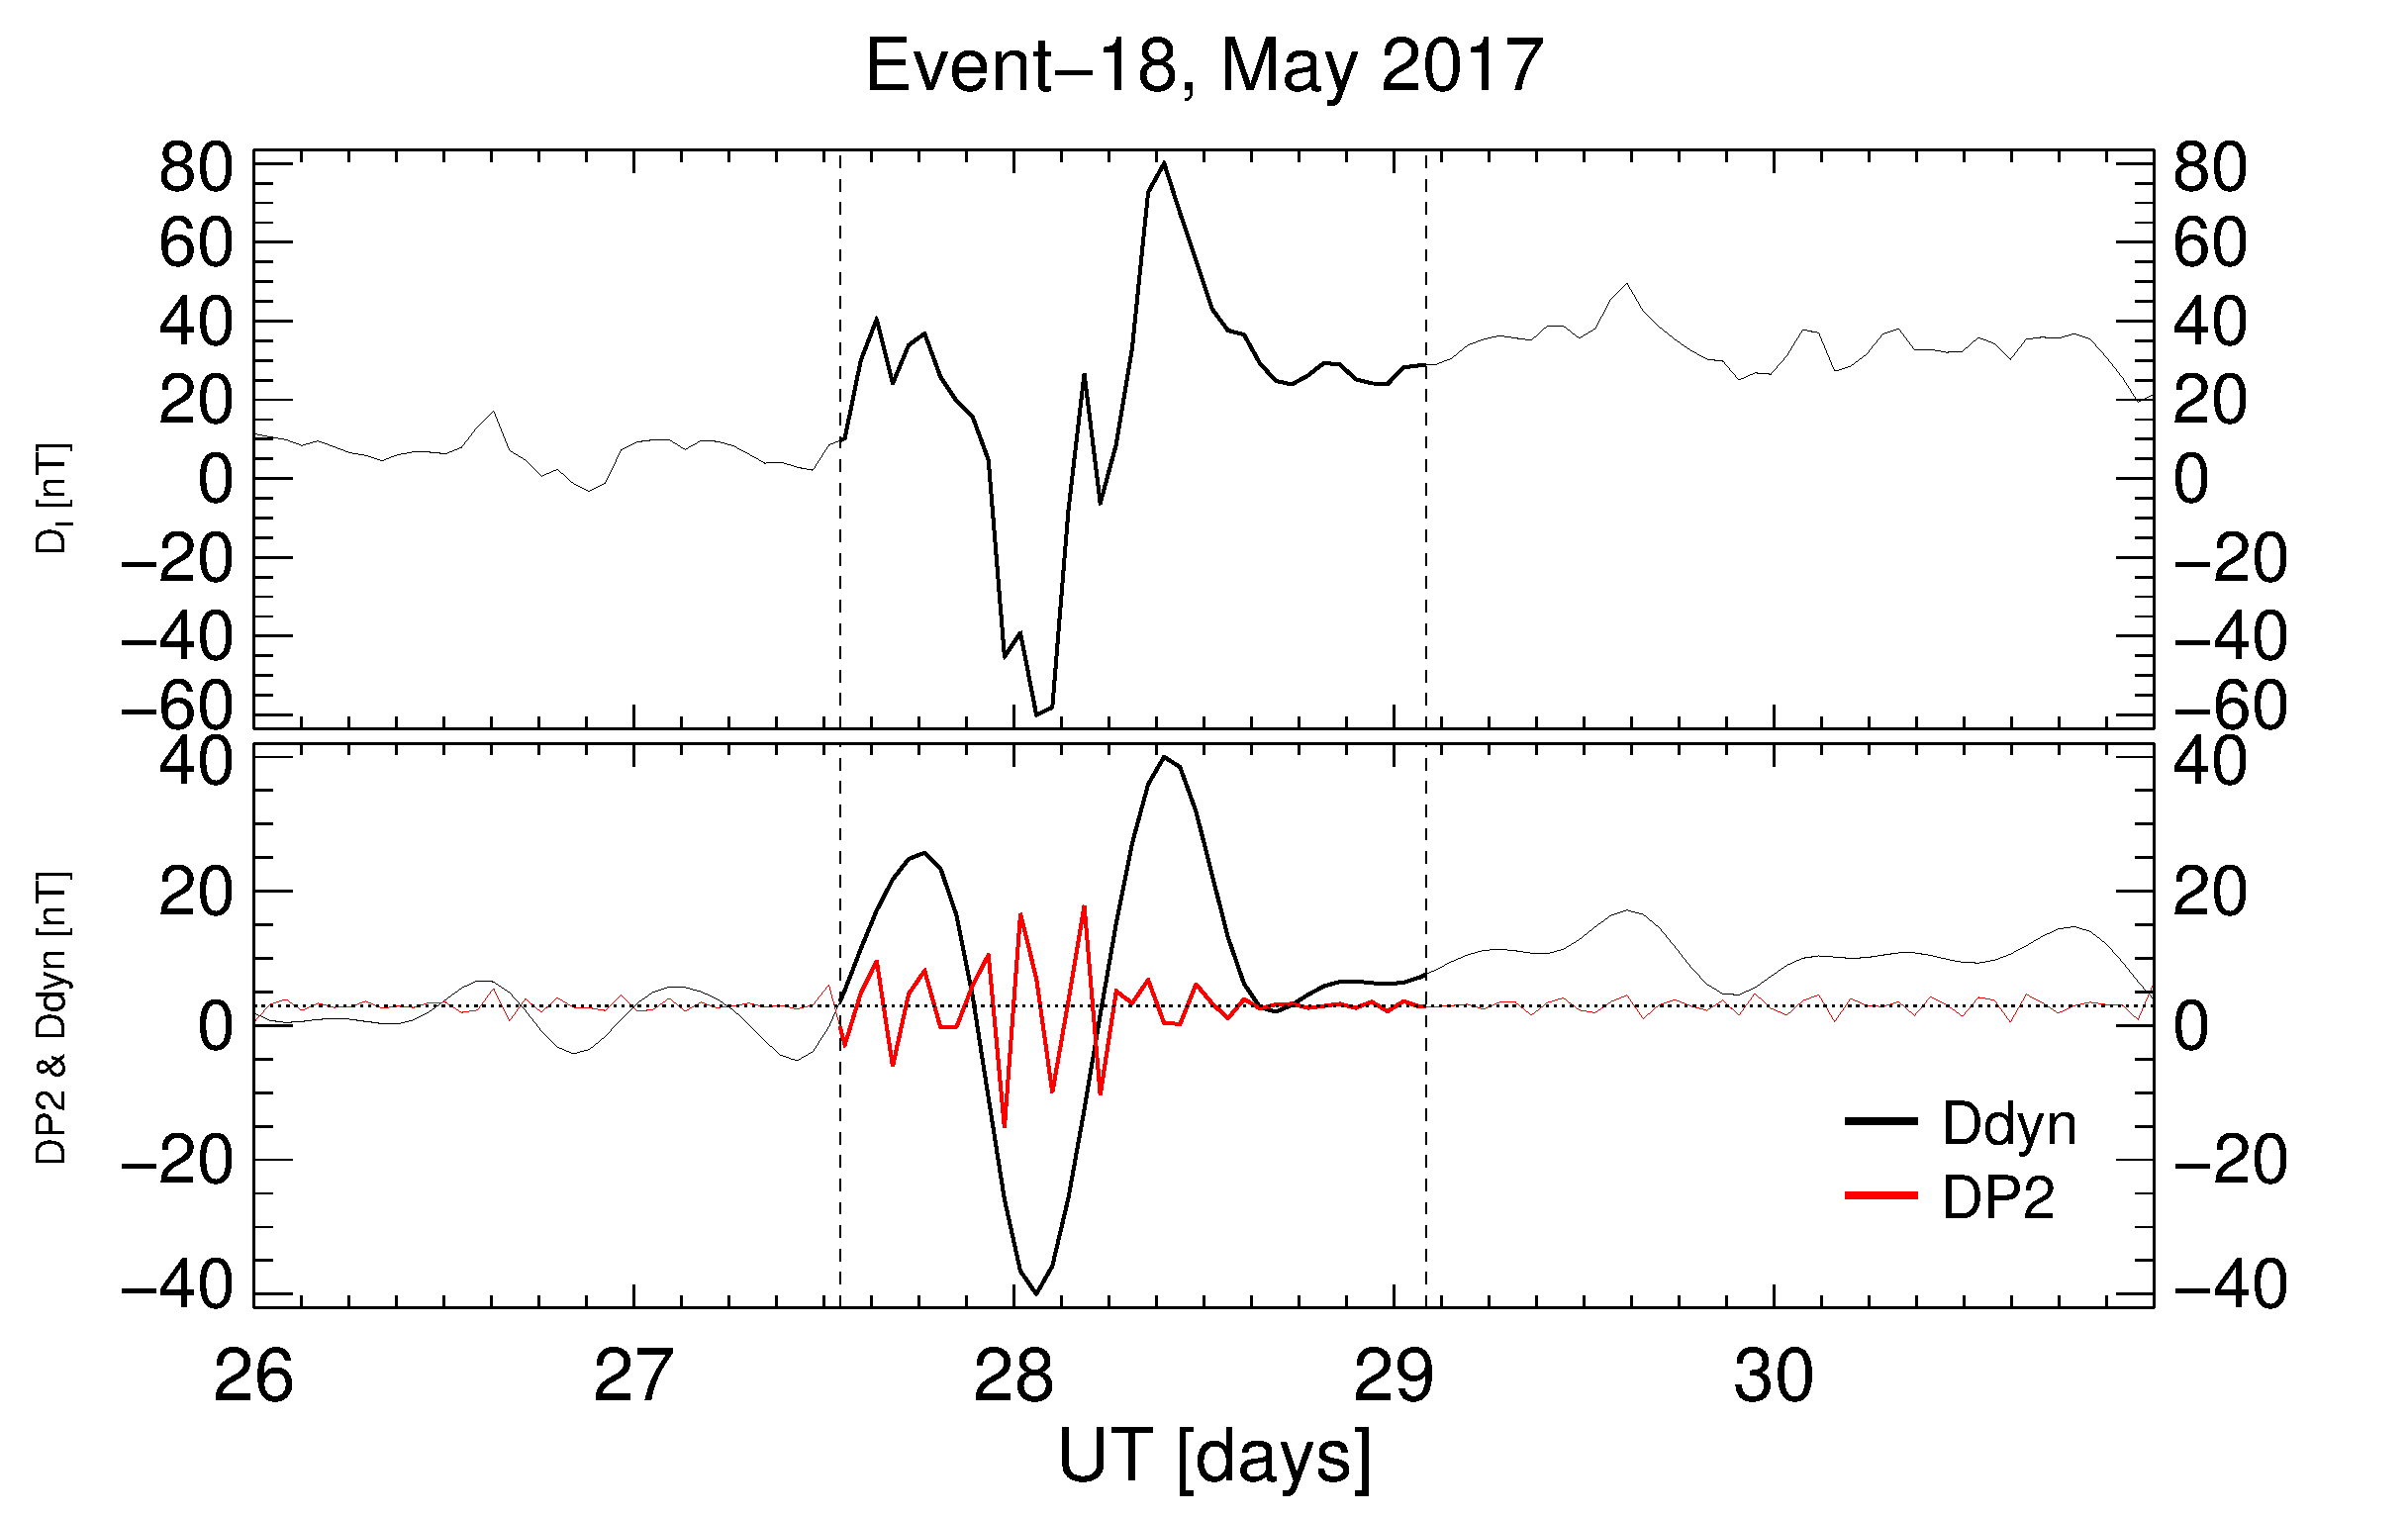
\includegraphics[width=6.0cm]{images/diono/iono_PI_V1_2017-05-26.eps}
    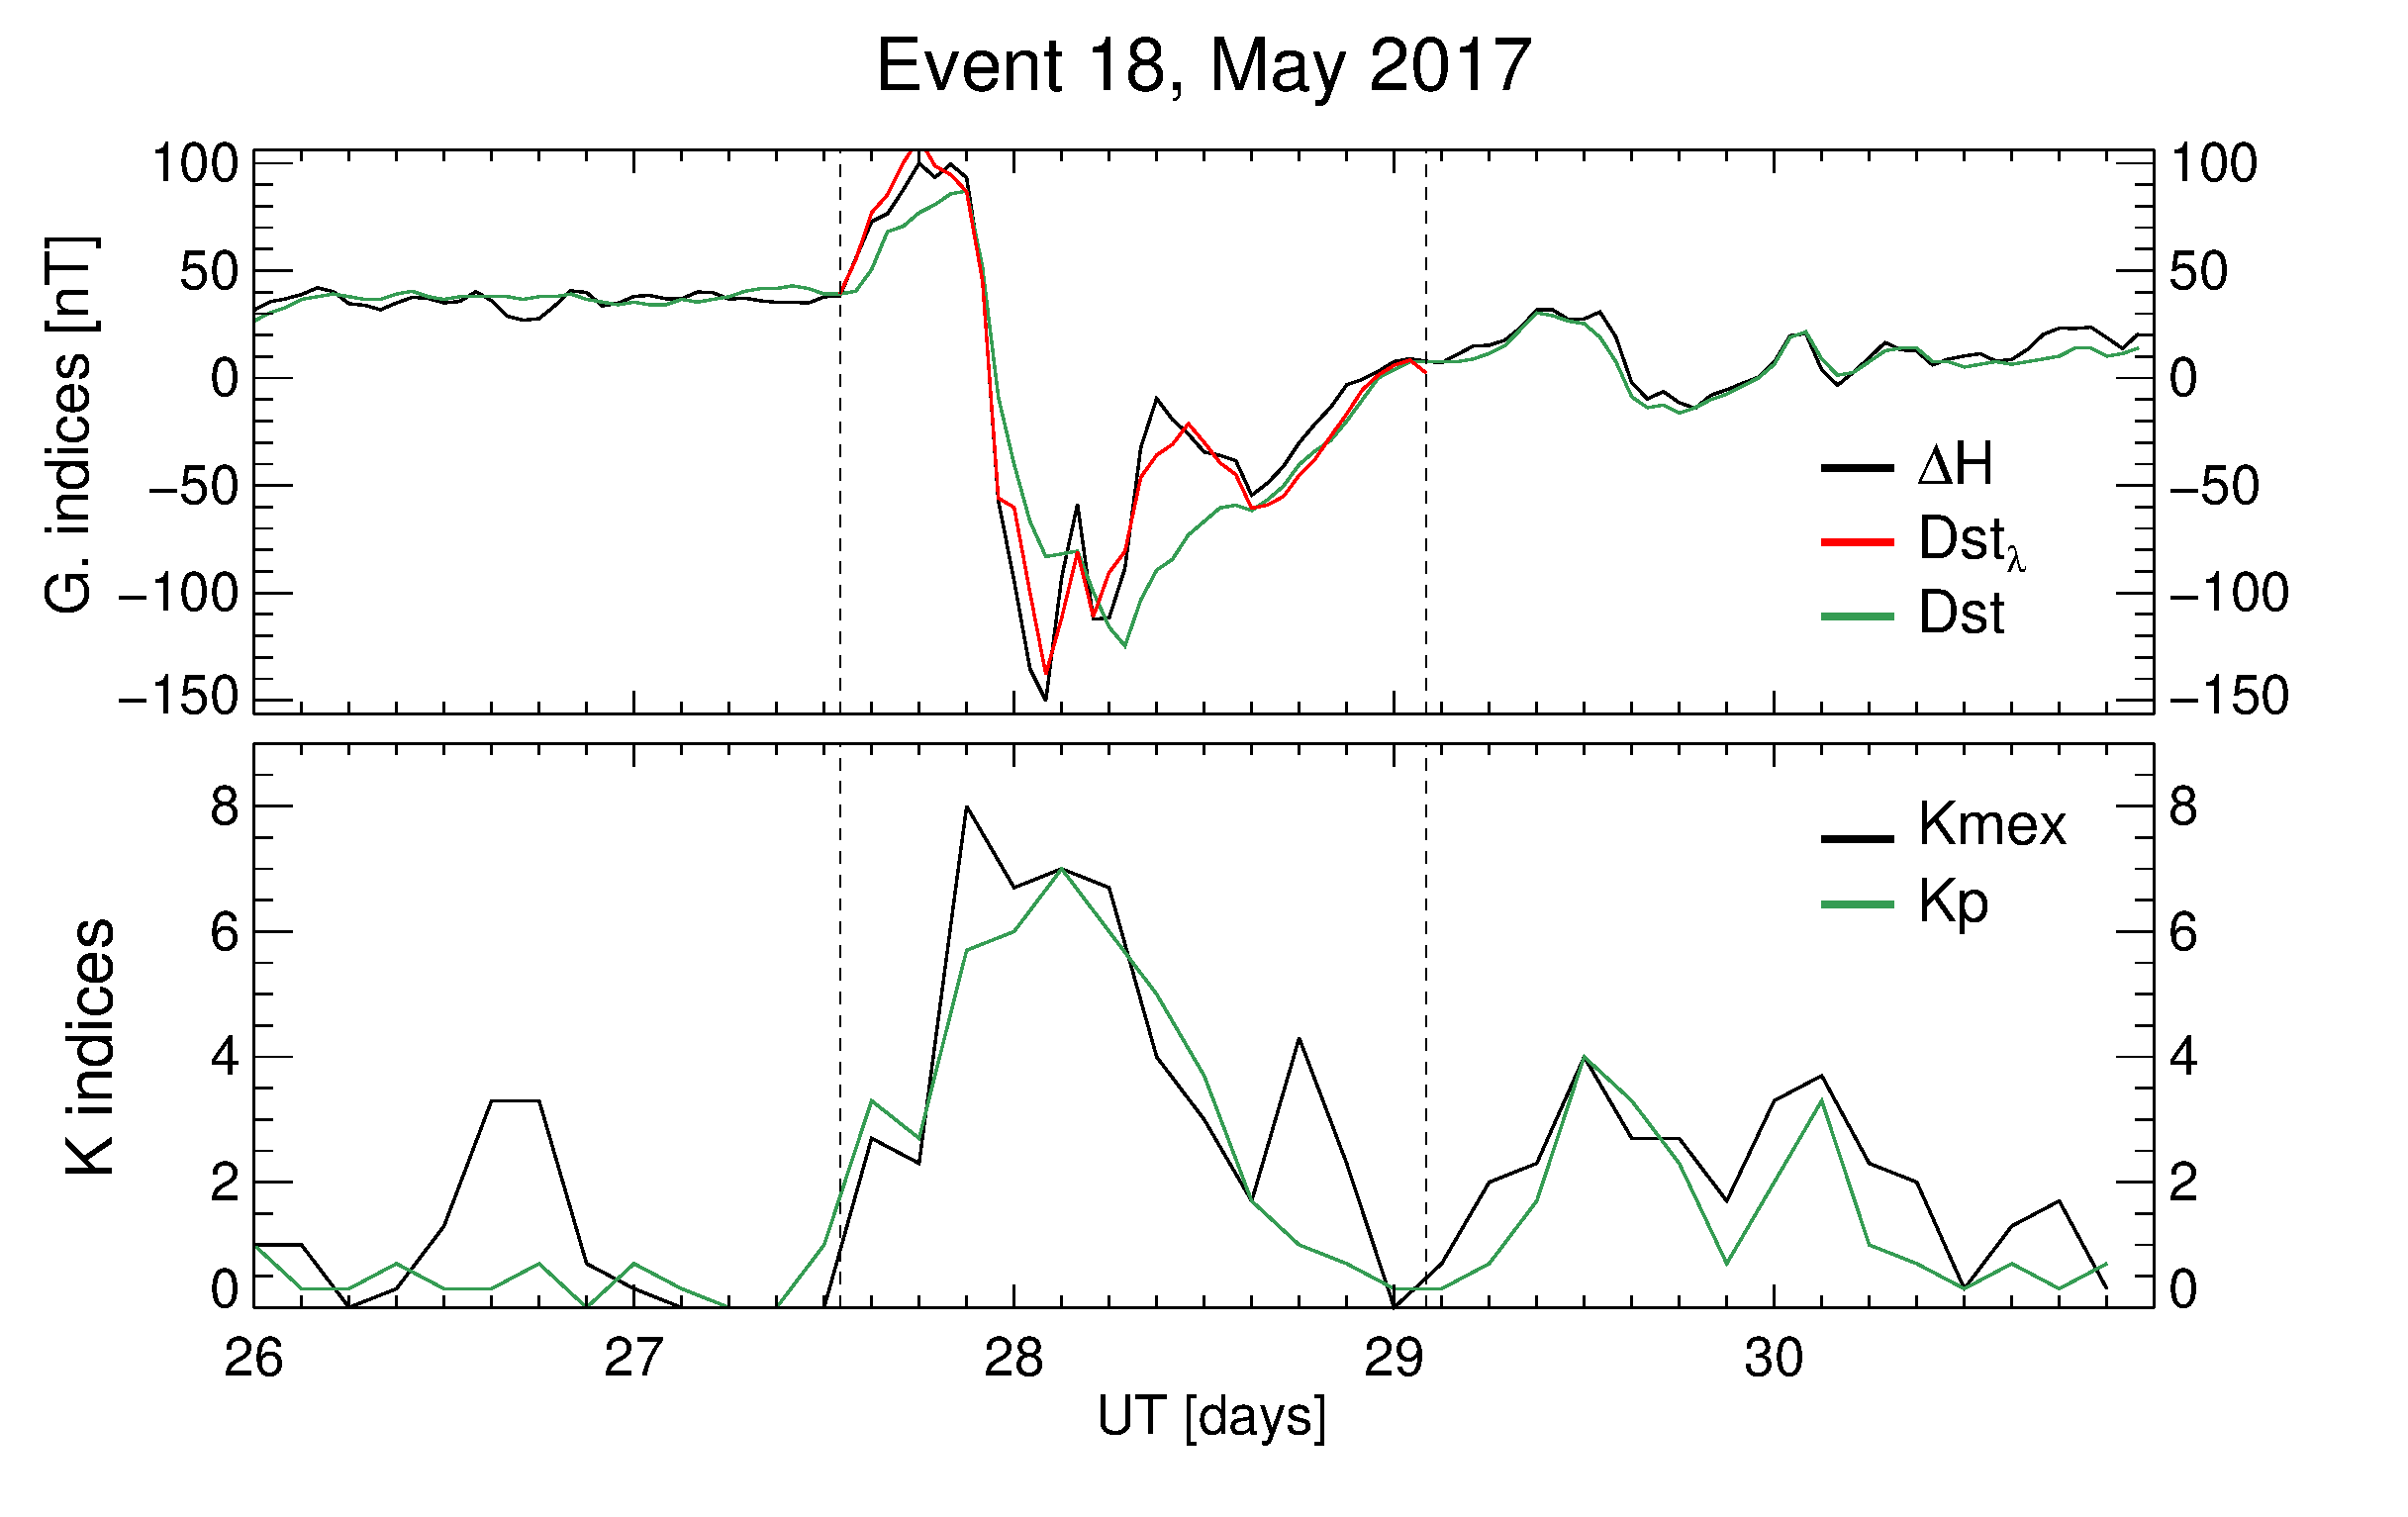
\includegraphics[width=6.0cm]{images/dH_approx/diono_valid_V4_2017-05-26.eps}

       \centerline{\Large \bf   
      \hspace{0.275\textwidth}  \color{black}{}
       \hspace{0.295\textwidth}  \color{black}{}
         \hfill}
    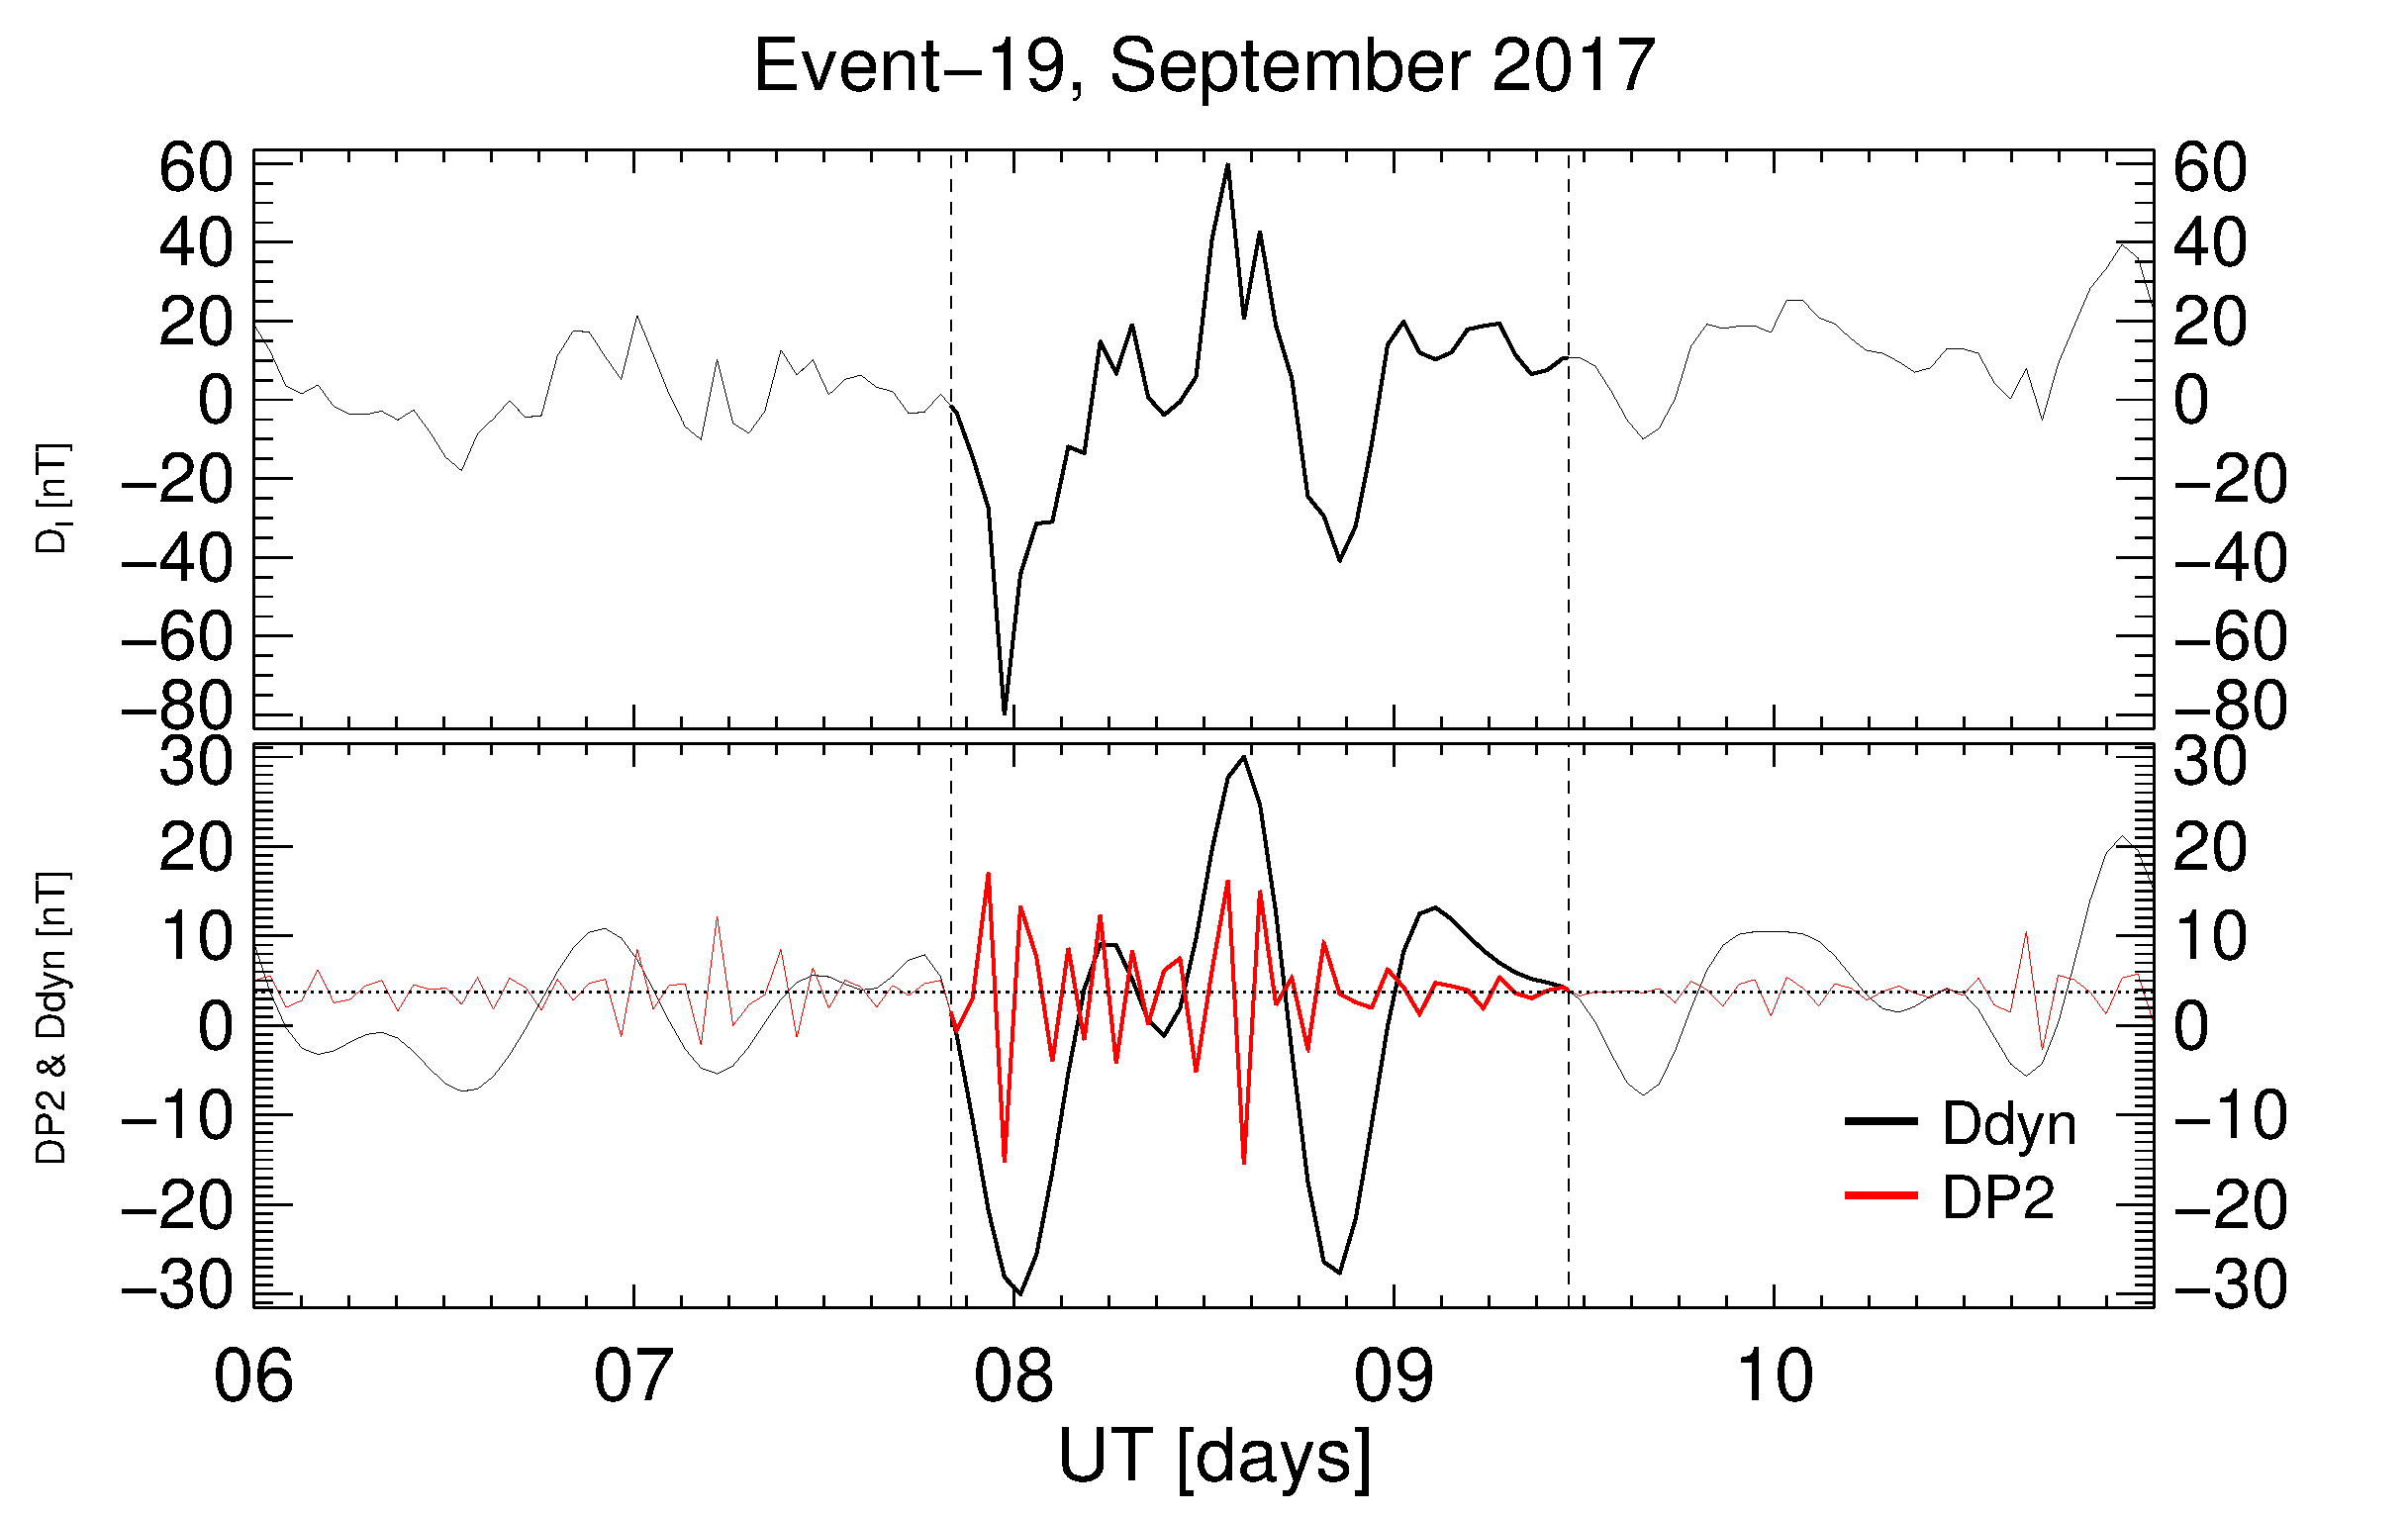
\includegraphics[width=6.0cm]{images/diono/iono_PI_V1_2017-09-06.eps}  
 	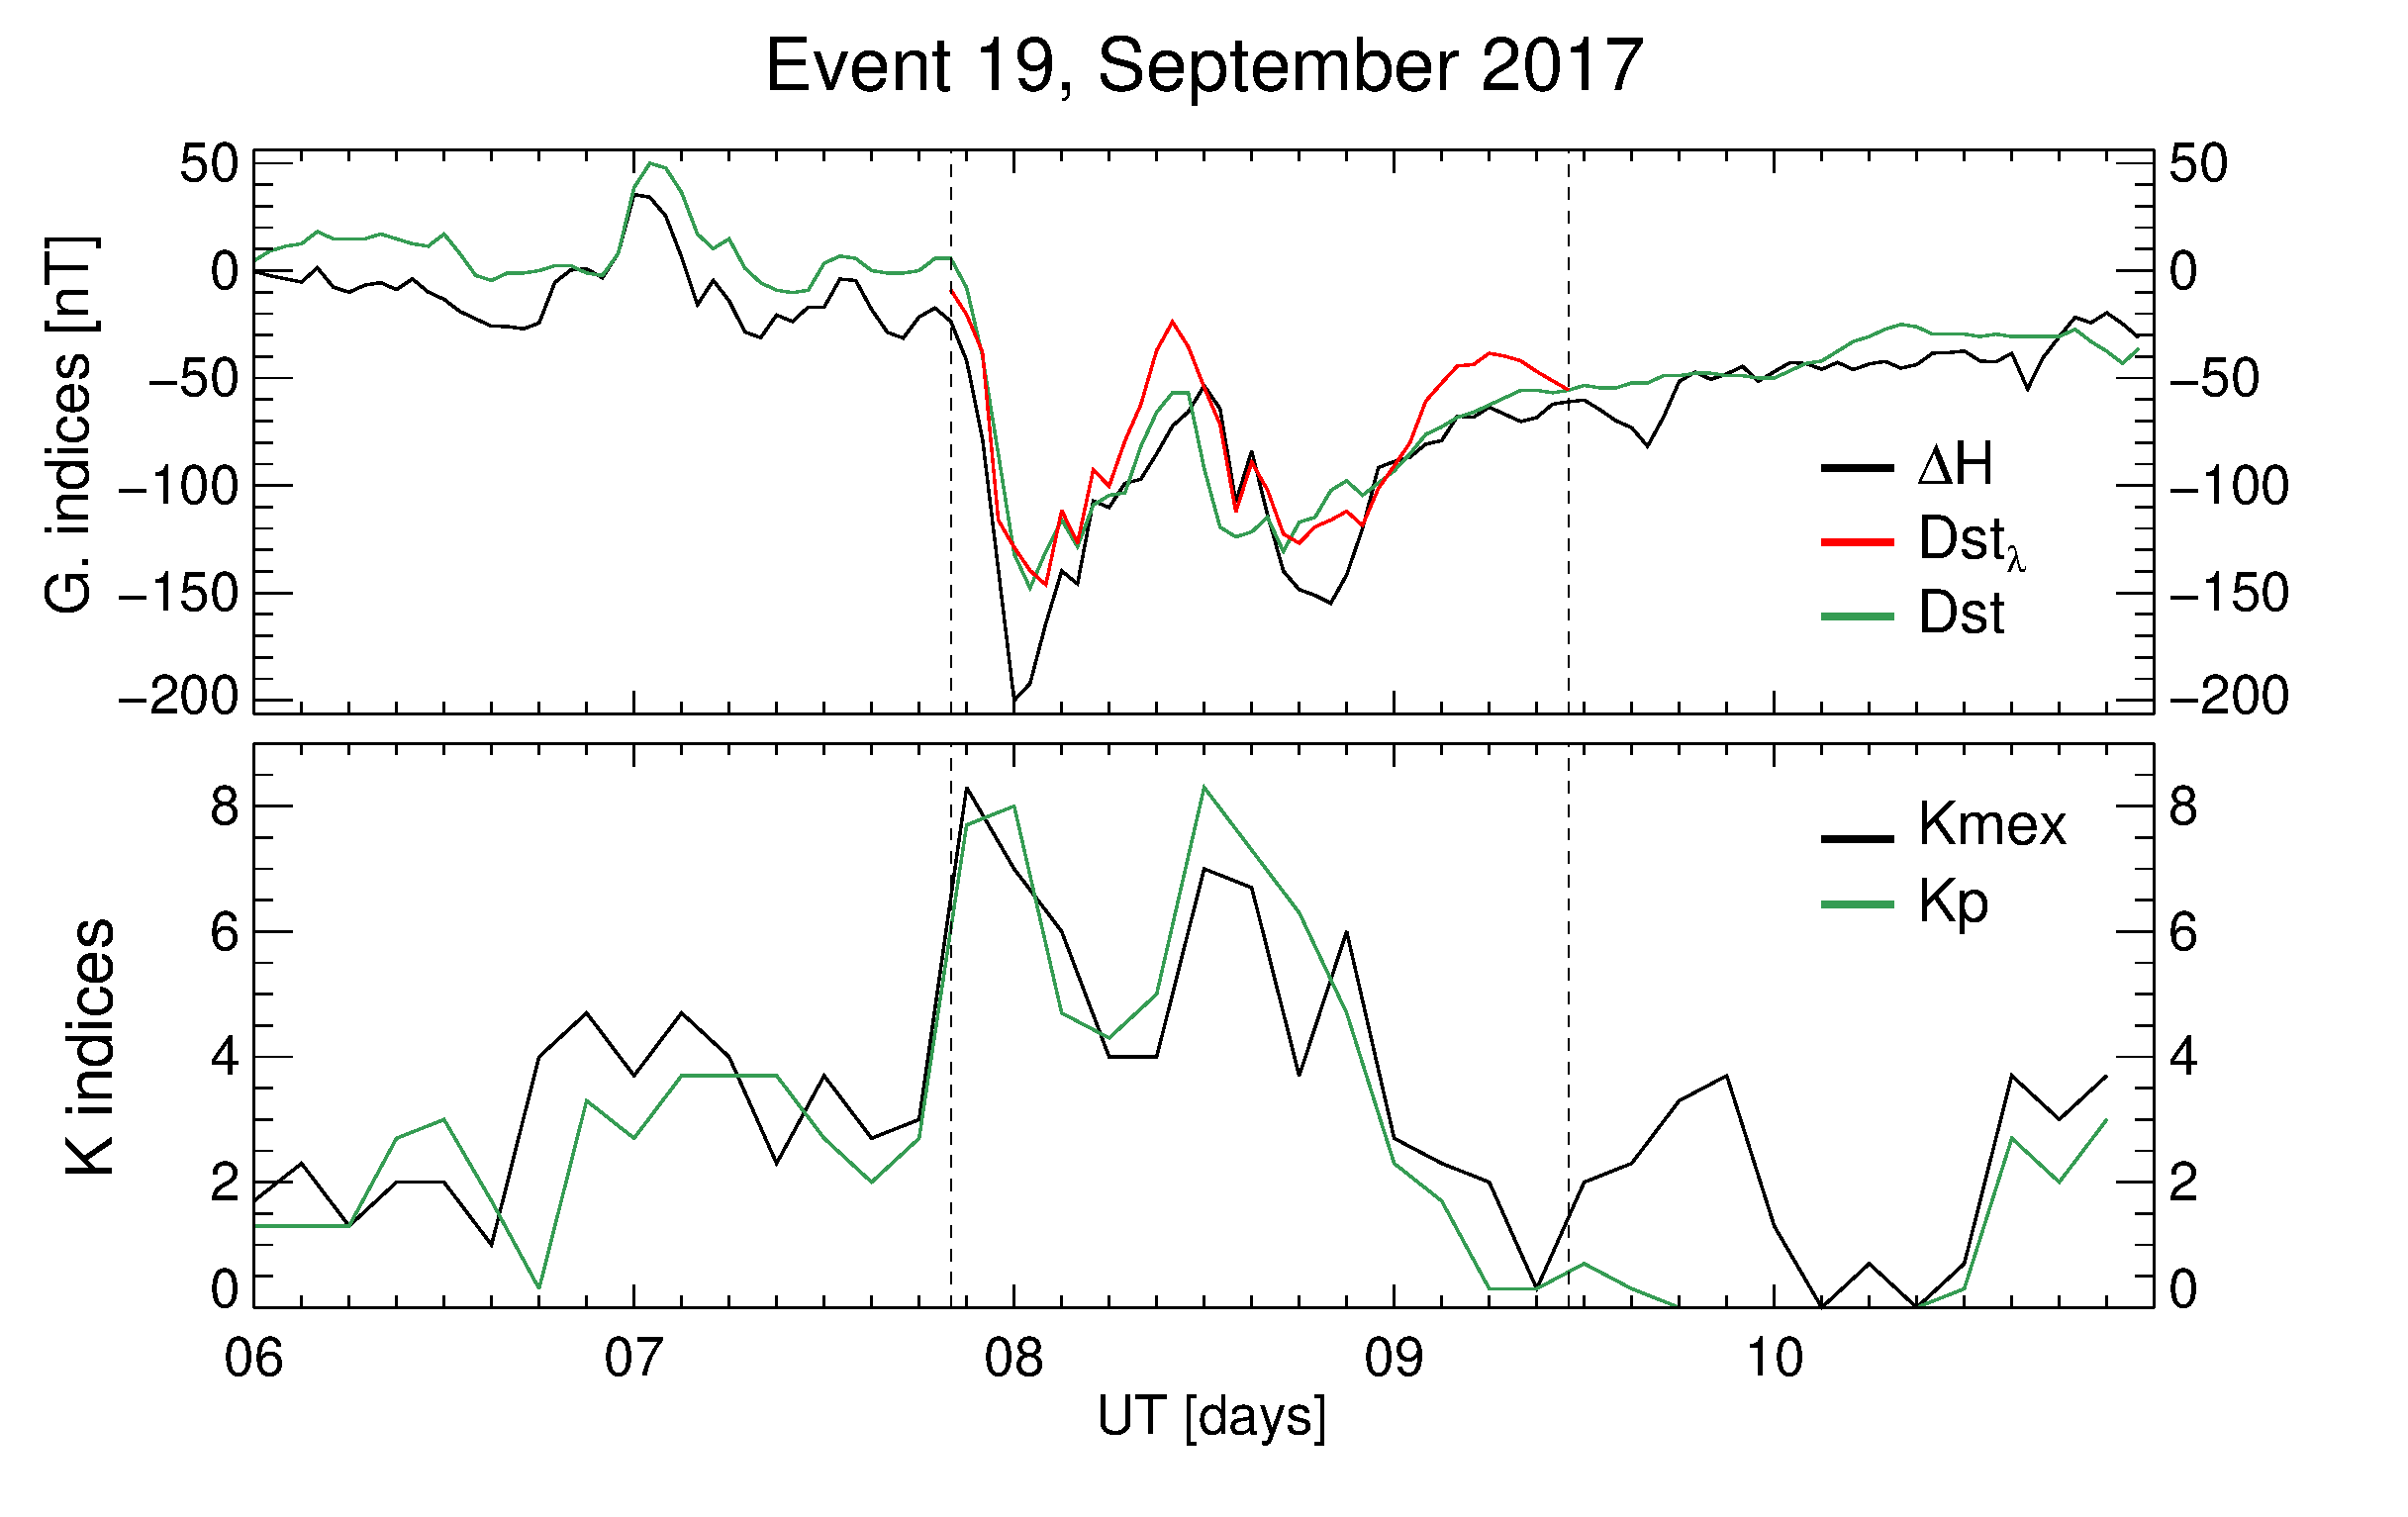
\includegraphics[width=6.0cm]{images/dH_approx/diono_valid_V4_2017-09-06.eps}    

       \centerline{\Large \bf   
      \hspace{0.275\textwidth}  \color{black}{}
       \hspace{0.295\textwidth}  \color{black}{}
         \hfill}
	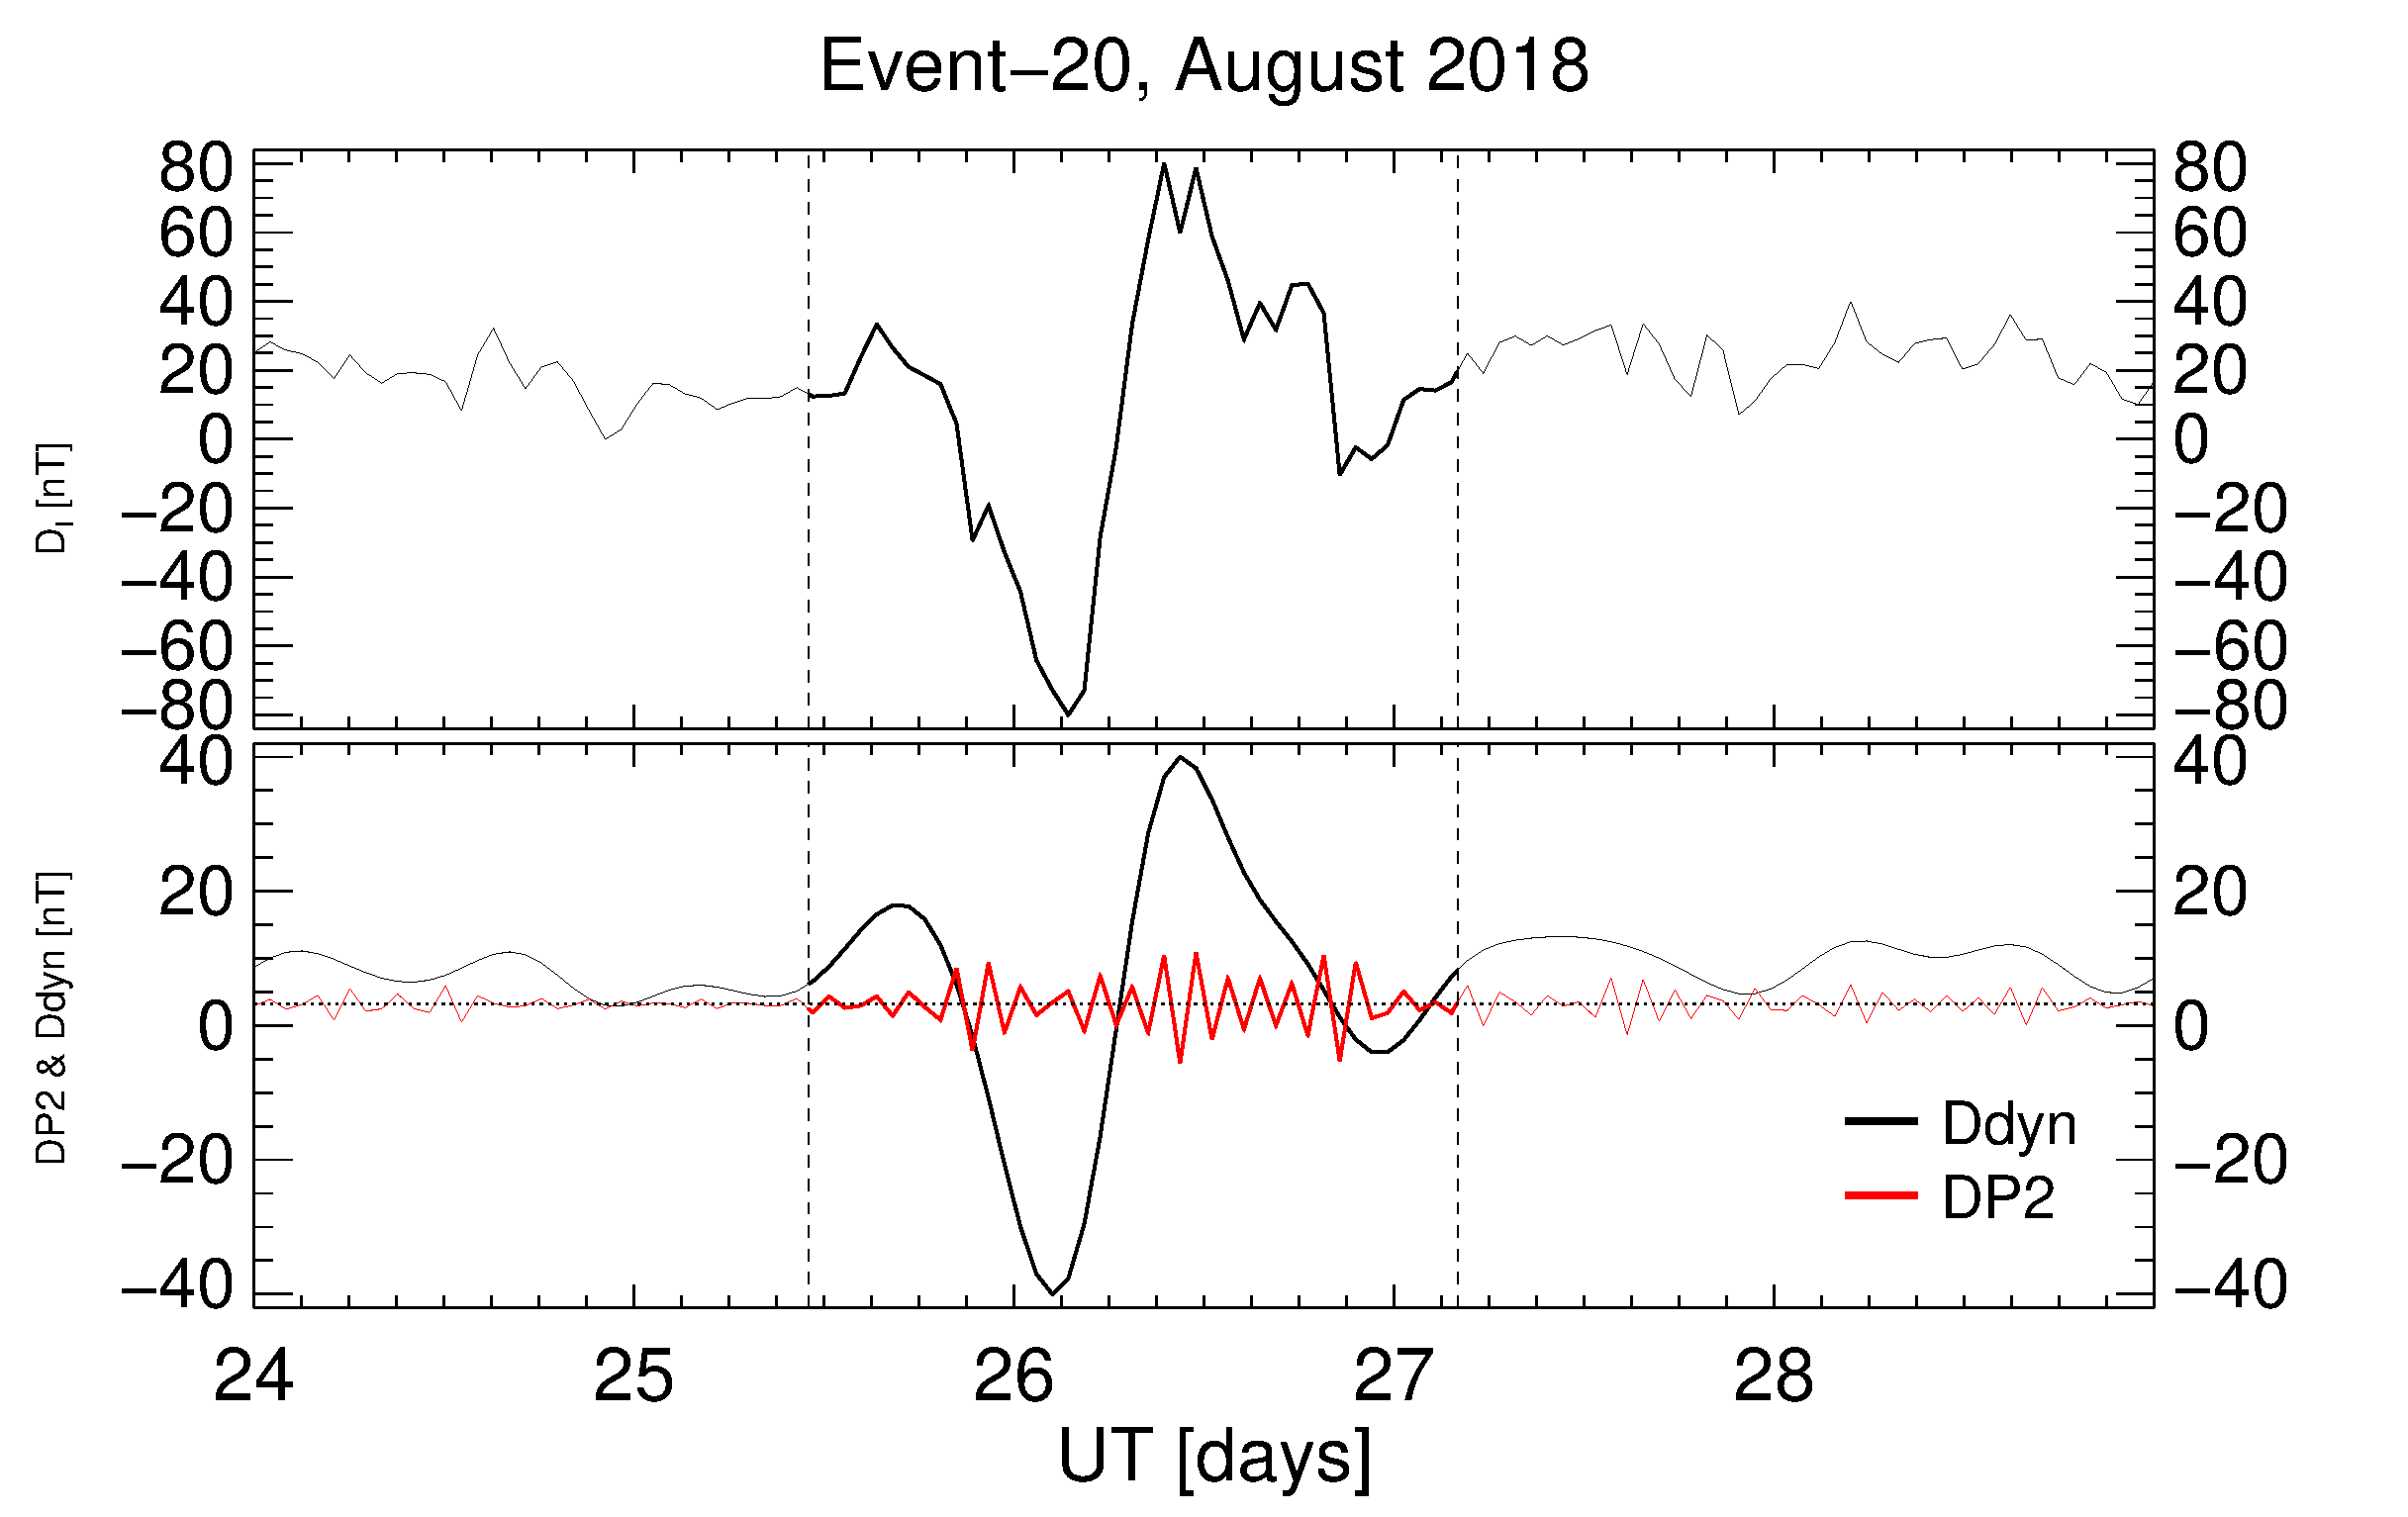
\includegraphics[width=6.0cm]{images/diono/iono_PI_V1_2018-08-24.eps}	
	\includegraphics[width=6.0cm]{images/dH_approx/diono_valid_V4_2018-08-24.eps}	
	       
       \caption{On the right side, top panels illustrate the contribution of Ionospheric Magnetic Disturbances, while bottom panels depict the isolated geomagnetic contributions of $Ddyn$ and $DP2$. The vertical dashed lines highlight the geomagnetic storm time period during which such calculations are valid. On the left side, green lines represent planetary indices, while black lines denote local indices. Additionally, red lines represent the approximation of $\Delta H$ at top, while bottom showcases the comparison of local $K$ (black line) and planetary $K$ (green line).
       }
    \label{fig:iono_valid3}
\end{figure*}


\end{document}

